% bmvc_supp.tex — supplementary material for the BMVC 2026 submission.
%
% Builds with `make supp`. Shares figures/ and the generated stat macros with
% the main paper, so a number cited here cannot drift from the same number in
% blob_boards_bmvc.tex: both \input the SAME bb_stats.tex / bb_occ_stats.tex,
% which `make floorplan` regenerates from the collected results frame.
\documentclass{bmvc2k}

\usepackage{cleveref}
\usepackage[section]{placeins}
\usepackage{graphicx}
\usepackage{booktabs}
\usepackage{amsmath}
\usepackage{amssymb}
\usepackage{bm}
\usepackage{algorithm}
\usepackage{algpseudocode}
\usepackage{pgfplots}
% S-prefixed counters so the main paper's cross-references (via xr-hyper)
% read as Section S3 / Figure S2 and cannot be confused with its own.
\renewcommand{\thesection}{S\arabic{section}}
\renewcommand{\thefigure}{S\arabic{figure}}
\renewcommand{\thetable}{S\arabic{table}}
\renewcommand{\theequation}{S\arabic{equation}}
\renewcommand{\thealgorithm}{S\arabic{algorithm}}
\pgfplotsset{compat=1.18}
\newcommand{\fpscale}{1}
\newcommand{\vtheta}{\bm{\theta}}
\newcommand{\va}{\bm{a}}

% Generated evaluation numbers — do not edit by hand; see
% bmvc2026/scripts/plots/error_distributions.jl.
% bb_stats.tex — generated by experiments/plots/error_distributions.jl
% every number the paper cites in prose; do not edit by hand
\newcommand{\bbDet}{80}
\newcommand{\bbAttTransMed}{4.5}
\newcommand{\bbAttRotMed}{0.58}
\newcommand{\bbTransMed}{3.8}
\newcommand{\bbRotMed}{0.46}
\newcommand{\bbDetLarge}{86}
\newcommand{\bbTransMedLarge}{5.0}
\newcommand{\bbRotMedLarge}{0.43}
\newcommand{\bbRotPninetyLarge}{0.98}
\newcommand{\bbDetMedium}{83}
\newcommand{\bbTransMedMedium}{3.7}
\newcommand{\bbRotMedMedium}{0.43}
\newcommand{\bbRotPninetyMedium}{0.99}
\newcommand{\bbDetSmall}{78}
\newcommand{\bbTransMedSmall}{3.6}
\newcommand{\bbRotMedSmall}{0.49}
\newcommand{\bbRotPninetySmall}{1.76}
\newcommand{\aprDet}{74}
\newcommand{\aprAttTransMed}{39.7}
\newcommand{\aprAttRotMed}{0.78}
\newcommand{\aprTransMed}{25.6}
\newcommand{\aprRotMed}{0.5}
\newcommand{\aprDetLarge}{84}
\newcommand{\aprTransMedLarge}{16.6}
\newcommand{\aprRotMedLarge}{0.35}
\newcommand{\aprRotPninetyLarge}{1.22}
\newcommand{\aprDetMedium}{76}
\newcommand{\aprTransMedMedium}{25.7}
\newcommand{\aprRotMedMedium}{0.44}
\newcommand{\aprRotPninetyMedium}{2.11}
\newcommand{\aprDetSmall}{69}
\newcommand{\aprTransMedSmall}{32.8}
\newcommand{\aprRotMedSmall}{0.63}
\newcommand{\aprRotPninetySmall}{24.74}
\newcommand{\ucoDet}{58}
\newcommand{\ucoAttTransMed}{62.9}
\newcommand{\ucoAttRotMed}{12.55}
\newcommand{\ucoTransMed}{19.0}
\newcommand{\ucoRotMed}{1.38}
\newcommand{\ucoDetLarge}{84}
\newcommand{\ucoTransMedLarge}{24.2}
\newcommand{\ucoRotMedLarge}{0.92}
\newcommand{\ucoRotPninetyLarge}{1.85}
\newcommand{\ucoDetMedium}{71}
\newcommand{\ucoTransMedMedium}{37.9}
\newcommand{\ucoRotMedMedium}{1.26}
\newcommand{\ucoRotPninetyMedium}{28.97}
\newcommand{\ucoDetSmall}{45}
\newcommand{\ucoTransMedSmall}{12.5}
\newcommand{\ucoRotMedSmall}{1.92}
\newcommand{\ucoRotPninetySmall}{40.44}
\newcommand{\bbScaleRotMedCeil}{0.5}
\newcommand{\gainAprLarge}{3.3}
\newcommand{\gainAprLargePct}{70}
\newcommand{\gainAprMedium}{6.9}
\newcommand{\gainAprMediumPct}{86}
\newcommand{\gainAprSmall}{9.1}
\newcommand{\gainAprSmallPct}{89}

% bb_occ_stats.tex — generated by error_distributions.jl
% occlusion numbers the paper cites in prose; do not edit by hand
\newcommand{\bbDetOccTen}{0.8}
\newcommand{\bbDetPctOccTen}{80}
\newcommand{\bbTransMedOccTen}{3.9}
\newcommand{\bbRotMedOccTen}{1.1}
\newcommand{\aprDetOccTen}{0.11}
\newcommand{\aprDetPctOccTen}{11}
\newcommand{\aprTransMedOccTen}{33.0}
\newcommand{\aprRotMedOccTen}{1.62}
\newcommand{\ucoDetOccTen}{0.23}
\newcommand{\ucoDetPctOccTen}{23}
\newcommand{\ucoTransMedOccTen}{91.2}
\newcommand{\ucoRotMedOccTen}{18.79}
\newcommand{\bbDetOccFifty}{0.69}
\newcommand{\bbDetPctOccFifty}{69}
\newcommand{\bbTransMedOccFifty}{3.9}
\newcommand{\bbRotMedOccFifty}{1.05}
\newcommand{\aprDetOccFifty}{0.0}
\newcommand{\aprDetPctOccFifty}{0}
\newcommand{\aprTransMedOccFifty}{3.2}
\newcommand{\aprRotMedOccFifty}{n/a}
\newcommand{\ucoDetOccFifty}{0.0}
\newcommand{\ucoDetPctOccFifty}{0}
\newcommand{\ucoTransMedOccFifty}{n/a}
\newcommand{\ucoRotMedOccFifty}{n/a}
\newcommand{\bbDetOccSeventy}{0.49}
\newcommand{\bbDetPctOccSeventy}{49}
\newcommand{\bbTransMedOccSeventy}{3.6}
\newcommand{\bbRotMedOccSeventy}{0.89}
\newcommand{\aprDetOccSeventy}{0.0}
\newcommand{\aprDetPctOccSeventy}{0}
\newcommand{\aprTransMedOccSeventy}{3.2}
\newcommand{\aprRotMedOccSeventy}{n/a}
\newcommand{\ucoDetOccSeventy}{0.0}
\newcommand{\ucoDetPctOccSeventy}{0}
\newcommand{\ucoTransMedOccSeventy}{n/a}
\newcommand{\ucoRotMedOccSeventy}{n/a}
\newcommand{\bbTransMedOccMin}{3.6}
\newcommand{\bbTransMedOccMax}{4.0}
\newcommand{\ucoZeroFromOccPct}{50}
\newcommand{\aprCollapseFromOccPct}{20}
\newcommand{\ucoCollapseFromOccPct}{30}
\newcommand{\bbMaxDetectedOccPct}{90}

% handeye_stats.tex — generated by scripts/make_handeye_table.jl; do not edit by hand
\newcommand{\bbHeFrames}{41}
\newcommand{\bbHeRecovered}{37}
\newcommand{\bbHeMarkers}{30}
\newcommand{\bbHeResidTransMM}{0.68}
\newcommand{\bbHeResidRotDeg}{0.27}
\newcommand{\aprHeFrames}{22}
\newcommand{\aprHeRecovered}{0}
\newcommand{\aprHeMarkers}{30}
\newcommand{\aprHeResidTransMM}{2.54}
\newcommand{\aprHeResidRotDeg}{0.432}
\newcommand{\ucoHeFrames}{15}
\newcommand{\ucoHeRecovered}{0}
\newcommand{\ucoHeMarkers}{30}
\newcommand{\ucoHeResidTransMM}{2.81}
\newcommand{\ucoHeResidRotDeg}{1.885}

% det_stats.tex — generated by scripts/make_detection_stats.jl
% detection counts from the promoted BlobBoards snapshot; do not edit by hand
\newcommand{\bbDetPoses}{1346}
\newcommand{\bbDetCaptures}{56}
\newcommand{\bbGalleryEval}{30}
\newcommand{\bbMinSpacingMM}{47.8}

% timing_stats.tex — generated by error_distributions.jl
% end-to-end per-image detection time from the promoted pose JSONs
\newcommand{\bbTimeMeanS}{2.03}
\newcommand{\bbTimeStdS}{2.18}
\newcommand{\bbTimeMedS}{1.84}
\newcommand{\bbTimeN}{56}
\newcommand{\aprTimeMeanS}{0.11}
\newcommand{\aprTimeStdS}{0.01}
\newcommand{\aprTimeMedS}{0.11}
\newcommand{\aprTimeN}{57}
\newcommand{\ucoTimeMeanS}{0.04}
\newcommand{\ucoTimeStdS}{0.01}
\newcommand{\ucoTimeMedS}{0.04}
\newcommand{\ucoTimeN}{57}

% board_params.tex — generated by bmvc2026/scripts/make_supp_tables.jl; do not edit by hand
% the evaluation gallery's pattern parameters, from <dataset>/boards/blobboards/*.json
\newcommand{\bbGalleryBoards}{30}
\newcommand{\bbBlobsMinAll}{202}
\newcommand{\bbBlobsMaxAll}{1032}
\newcommand{\bbBoardsSmall}{18}
\newcommand{\bbExtentMMSmall}{40}
\newcommand{\bbBlobsMedSmall}{213}
\newcommand{\bbBlobsMinSmall}{202}
\newcommand{\bbBlobsMaxSmall}{226}
\newcommand{\bbBoardsMedium}{8}
\newcommand{\bbExtentMMMedium}{60}
\newcommand{\bbBlobsMedMedium}{374}
\newcommand{\bbBlobsMinMedium}{365}
\newcommand{\bbBlobsMaxMedium}{390}
\newcommand{\bbBoardsLarge}{4}
\newcommand{\bbExtentMMLarge}{120}
\newcommand{\bbBlobsMedLarge}{1023}
\newcommand{\bbBlobsMinLarge}{1001}
\newcommand{\bbBlobsMaxLarge}{1032}
\newcommand{\bbPatMinScaleMM}{0.2}
\newcommand{\bbPatMaxDiamFrac}{0.5}
\newcommand{\bbPatCutoff}{2}
\newcommand{\bbPatAlpha}{1.6}
\newcommand{\bbPatScalesPerOctave}{3}
\newcommand{\bbPatDPI}{1200}
\newcommand{\bbPatPolarity}{dark}

% run_settings.tex — generated by bmvc2026/scripts/make_supp_tables.jl; do not edit by hand
% operational settings of the promoted run, from <dataset>/poses/bb/_config.toml via FindBoardsConfig
\newcommand{\bbSetWarps}{25}
\newcommand{\bbSetTiltOne}{2.62}
\newcommand{\bbSetTiltAnglesOne}{8}
\newcommand{\bbSetTiltTwo}{5.18}
\newcommand{\bbSetTiltAnglesTwo}{16}
\newcommand{\bbSetPeakThreshold}{0.01}
\newcommand{\bbSetEdgeThreshold}{5.0}
\newcommand{\bbSetNmsCutoff}{2.0}
\newcommand{\bbSetScanWindow}{2.0}
\newcommand{\bbSetMaxIrls}{20}
\newcommand{\bbSetRtol}{10^{-6}}
\newcommand{\bbSetMaxScaleFraction}{0.1}
\newcommand{\bbSetMaxScaleRatio}{4}
\newcommand{\bbSetMaxClipRatio}{0.2}
\newcommand{\bbSetMaxAspectRatio}{10}
\newcommand{\bbSetInnerRadius}{2.0}
\newcommand{\bbSetMinSimilarity}{0.6}
\newcommand{\bbSetMinInliers}{9}
\newcommand{\bbSetHalfwidthPx}{5}
\newcommand{\bbSetRansacMin}{100}
\newcommand{\bbSetRansacMax}{2000}
\newcommand{\bbSetConfidence}{0.99}
\newcommand{\bbSetAppearanceSupportPct}{50}
\newcommand{\bbSetVerifySimilarity}{0.6}


% Title card: same author/institution layout as the main paper, so the two
% documents present identically. Kept in sync by hand with
% blob_boards_bmvc.tex.
% --- compact title card ---------------------------------------------------
% bmvc2k stacks one author per line in a 0.49\textwidth column, plus an empty
% e-mail line under each (all seven \addauthor entries pass an empty mail), so
% seven authors cost ~14 lines. Flow the names into two columns instead and
% give the single institution the rest of the width. Two columns (not three)
% because a full-width address such as jpr@informatik.uni-kiel.de overruns a
% third-width cell: the name/mail boxes are pre-packed \hbox es, so the
% overrun laps the neighbouring cell silently instead of reporting an
% overfull box. \addauthor and
% \addinstitution stay the source of truth; only the layout is overridden.
\makeatletter
% Record whether each author was given a mail argument, so the card can drop
% the second line for authors who have none instead of leaving a blank line.
\let\bmv@origaddauthor\addauthor
\def\addauthor#1#2#3{%
  \bmv@origaddauthor{#1}{#2}{#3}%
  \def\bmv@tmpmail{#2}%
  \expandafter\xdef\csname bmv@hasmail\the\bmv@nauthors\endcsname
    {\ifx\bmv@tmpmail\@empty 0\else 1\fi}}
\def\bmv@RenderInst#1{%
  \begin{minipage}[t]{0.28\textwidth}
    \sffamily
    \begin{raggedright}#1\end{raggedright}
  \end{minipage}}
\newcount\bmv@authcol
% The LAST author is set under the institution rather than alone on a short
% final row: with an odd author count the two-up grid otherwise leaves a
% half-empty row beside an equally empty institution column.
\newcount\bmv@gridauthors
\AtBeginDocument{\bmv@gridauthors=\bmv@nauthors \advance\bmv@gridauthors-1}
\def\bmv@authorcell#1{%
  \bmv@usebox{authname#1}%
  \ifnum\csname bmv@hasmail#1\endcsname=1
    \\ \bmv@usebox{authmail#1}%
  \fi}
\def\bmv@RenderAuthInstTwoColumn{%
  \begin{minipage}[t]{0.70\textwidth}
    \raggedright
    \bmv@authcol=0
    \def\bmv@action##1{%
      \ifnum##1>\bmv@gridauthors\else
        \begin{minipage}[t]{0.5\linewidth}%
          \raggedright
          \bmv@authorcell{##1}%
        \end{minipage}%
        \global\advance\bmv@authcol1
        \ifnum\bmv@authcol=2
          \global\bmv@authcol=0
          \ifnum##1<\bmv@gridauthors \\[3pt] \fi
        \fi
      \fi}%
    \def\bmv@between{}%
    \expandafter\bmv@maplistaux\bmv@auths\bmv@endstop
  \end{minipage}\hfill
  \begin{minipage}[t]{0.28\textwidth}
    \raggedright
    \def\bmv@action##1{\bmv@unhbox{inst##1}}%
    \def\bmv@between{\\[4pt]}%
    \expandafter\bmv@maplistaux\bmv@insts\bmv@endstop
    \\[\dimexpr2\baselineskip+3pt\relax]
    \bmv@authorcell{\the\bmv@nauthors}%
  \end{minipage}}
\makeatother

\addauthor{James Pritts}{jpr@informatik.uni-kiel.de}{1}
\addauthor{Till Sittart}{till.sittart@till-s.de}{1}
\addauthor{Hendrik Sauer}{hendrik-sauer@mailbox.org}{1}
\addauthor{Silja Jan\ss{}en}{sja@informatik.uni-kiel.de}{1}
\addauthor{Felix Seegr\"aber}{fse@informatik.uni-kiel.de}{1}
\addauthor{David Nakath}{dna@cs.uni-kiel.de}{1}
\addauthor{Kevin K\"oser}{kk@informatik.uni-kiel.de}{1}

\addinstitution{
 Marine Data Science\\
 Kiel University
}

\title{BlobBoards: {\large Supplementary Material}}
\runninghead{Pritts \bmvaEtAl}{BlobBoards Supplementary Material}

\begin{document}
\setlength{\emergencystretch}{3pt}% absorb sub-3pt overfulls (typeset polish)
\maketitle

\section{Board Generation}
\label{sec:supp:generation}

\Cref{alg:gen} states the placement procedure. Blobs are placed largest-first
by rejection sampling with disjoint supports; the coarse-to-fine order matters,
because placing small blobs first leaves no room for large ones and yields a
substantially sparser board.


\begin{algorithm}[!ht]
	\caption{Greedy coarse-to-fine board generation: blobs are placed
		largest-first by rejection sampling with disjoint supports, then
		rasterised in a single pass.}
	\label{alg:gen}
	\begin{algorithmic}[1]
		\Require board size $W\!\times\!H$; scale schedule
		$\sigma_1>\sigma_2>\dots>\sigma_n$ with target counts $m_i$; seed
		\Ensure pattern image $P$; blob set $\mathcal{B}=\{(\mathbf{c}_j,\sigma_j)\}$
		\State $\mathcal{T}\gets$ empty R-tree of placed supports;\ \ $\mathcal{B}\gets\varnothing$
		\For{$i=1,\dots,n$ \textbf{(coarse-to-fine)} and $k=1,\dots,m_i$}
		\Comment{largest blobs first}
		\Repeat
		\State sample centre $\mathbf{c}$ uniformly within the inset board
		\If{support disc of $(\mathbf{c},\sigma_i)$ overlaps no blob in $\mathcal{T}$}
		\State insert $(\mathbf{c},\sigma_i)$ into $\mathcal{T}$ and $\mathcal{B}$
		\EndIf
		\Until{placed \textbf{or} trial budget exhausted}
		\Comment{skip if no free spot found}
		\EndFor
		\State $P\gets\mathbf{1}_{H\times W}$
		\Comment{white background: the $\|\mathbf{x}\|\!\to\!c\sigma$ limit of the blob profile}
		\State rasterise every blob in $\mathcal{B}$ over its support
		\Comment{disjoint supports $\Rightarrow$ single pass}
		\State \Return $P,\ \mathcal{B}$
	\end{algorithmic}
\end{algorithm}

\section{Board Generation Settings}
\label{sec:supp:params}

\Cref{tab:supp:params} lists the pattern parameters used to generate every
BlobBoard in the evaluation. All three physical sizes share one parameter set;
only the pattern extent differs, so the number of blobs a board carries grows
with its area. A tag of the same physical size contributes four corners at
every size.

\begin{table}[!h]
	\centering\small
	\begin{tabular}{@{}lccc@{}}
		\toprule
		                                   & small     & medium   & large    \\
		\midrule
		pattern extent (mm)                & $\bbExtentMMSmall$      & $\bbExtentMMMedium$     & $\bbExtentMMLarge$    \\
		blobs per board (median)           & $\bbBlobsMedSmall$     & $\bbBlobsMedMedium$    & $\bbBlobsMedLarge$   \\
		\midrule
		\multicolumn{4}{@{}l}{\emph{shared across all sizes}}                \\
		minimum blob scale $s_{\min}$      & \multicolumn{3}{c}{$\bbPatMinScaleMM$\,mm}   \\
		maximum diameter fraction $d_f$    & \multicolumn{3}{c}{$\bbPatMaxDiamFrac$}       \\
		support cutoff $c$          & \multicolumn{3}{c}{$\bbPatCutoff$}         \\
		scale-sampling distribution $\alpha$       & \multicolumn{3}{c}{$\bbPatAlpha$}       \\
		scales per octave                  & \multicolumn{3}{c}{$\bbPatScalesPerOctave$}         \\
		print density                      & \multicolumn{3}{c}{$\bbPatDPI$\,dpi} \\
		polarity                           & \multicolumn{3}{c}{\bbPatPolarity}        \\
		\bottomrule
	\end{tabular}
	\caption{Pattern-generation settings for the evaluation boards ($\bbBoardsSmall$ small,
		$\bbBoardsMedium$ medium, $\bbBoardsLarge$ large). Each board is generated from its own random
		seed, so blob counts vary slightly within a size class; the ranges are
		$\bbBlobsMinSmall$--$\bbBlobsMaxSmall$, $\bbBlobsMinMedium$--$\bbBlobsMaxMedium$, and $\bbBlobsMinLarge$--$\bbBlobsMaxLarge$.}
	\label{tab:supp:params}
\end{table}

\section{Finite-Support Scale Correction}
\label{sec:supp:scalecorr}

Truncating the Gaussian at $c$ and removing the pedestal
$p=e^{-c^2/2}$ perturbs the scale-space response. Writing
$\rho=\sigma/\sigma_0$, $\kappa=c^2(1+\rho^2)/2\rho^2$ and
$q=e^{-\kappa}$, the centre response of the truncated profile is
\begin{equation}
	R(\mathbf{0},\sigma)
	\;=\; \frac{A}{1-p}\left[
		\frac{2\bigl(1-(1+\kappa)q\bigr)}{(1+\rho^2)^2}
		\;-\; \frac{2(1-q)}{1+\rho^2}
		\;+\; \frac{c^2\,q}{\rho^2}
		\right],
	\label{eq:supp:truncresponse}
\end{equation}
which recovers the ideal Laplacian-of-Gaussian response
$-2A\sigma_0^2\sigma^2/(\sigma_0^2+\sigma^2)^2$ as $c\to\infty$. Its
extremum lies at $\beta(c)\,\sigma_0$, where $\beta(c)$ is the pedestal
scale bias of the main paper,
$\beta(c)=\arg\max_{\rho}|R(\mathbf{0},\rho\sigma_0)|$. Because $\beta$
depends only on $c$, the truncated response is still scale-covariant
with a peak magnitude independent of $\sigma_0$, so dividing each detected
scale by $\beta(c)$ recovers $\sigma_0$ exactly under this continuous
model.

\section{Descriptor Training: Reference and Observation Patches}
\label{sec:supp:training}

At test time a query patch cropped from an image is matched against a
descriptor computed from the reference pattern, so the training objective
must contain that pairing explicitly. It does. For every board, reference
patches are rendered from the reference pattern and the known blob geometry, and are
written into the same patch tensor as the real observations, keyed by the same
$(\text{board hash},\,\text{blob index})$ identity. A reference patch is
therefore an ordinary member of its supervised-contrastive class: it serves as
an anchor whose positives are the real observations of that blob, and as a
positive when a real observation is the anchor.

The batch sampler ensures that reference patches are available for real patches by concatenating the patches for all tracks sharing a blob id including the reference patch and treating them as a unit. Unmatched detections enter each batch as confusers with unique singleton labels: they never act as anchors and never supply positives, appearing only in other anchors' negative denominators.  A batch is made up of \(1/2\) continuous sequences, and \(1/2\) confusers.

\section{Detection, Matching and Verification Settings}
\label{sec:supp:settings}

\Cref{tab:supp:settings} lists every operational parameter of the pipeline as
run for the results in this paper. These are transcribed from the run
configuration shipped with the released dataset record, which each driver
copies beside its output, so a run's artifacts always carry the configuration
that produced them.

\begin{table}[!ht]
	\centering\small
	\begin{tabular}{@{}llp{0.42\linewidth}@{}}
		\toprule
		stage                    & parameter                       & value                                                                       \\
		\midrule
		detect                   & affine warps                    & IMAS-$\bbSetWarps$: identity, plus tilt $\bbSetTiltOne$ at $\bbSetTiltAnglesOne$ angles $\pi k/8$ and tilt $\bbSetTiltTwo$ at $\bbSetTiltAnglesTwo$ angles $\pi k/16$ \\
		                         & pre-upsampling                  & $2\times$ (scale space starts at octave $-1$)                               \\
		                         & DoG peak threshold              & $\bbSetPeakThreshold$                                                                      \\
		                         & DoG edge threshold              & $\bbSetEdgeThreshold$                                                                       \\
		                         & cross-warp NMS                  & elliptical, Mahalanobis cutoff $\bbSetNmsCutoff$                                        \\
		                         & detections kept                 & unbounded (no response-rank cap)                                            \\
		\midrule
		adapt                    & scan window                     & $\bbSetScanWindow\,\sigma$                                                               \\
		                         & max IRLS iterations             & $\bbSetMaxIrls$                                                                        \\
		                         & convergence tolerance           & $\bbSetRtol$ relative                                                          \\
		                         & storage / accumulation          & \texttt{Float32} / \texttt{Float64}                                         \\
		                         & validity guards                 & scale $\le\bbSetMaxScaleFraction\sqrt{WH}$, scale ratio $\le\bbSetMaxScaleRatio$, clip ratio $\le\bbSetMaxClipRatio$, aspect $\le\bbSetMaxAspectRatio$ \\
		\midrule
		canonicalize             & log-polar grid                  & $64\times64$                                                                \\
		                         & inner radius                    & $c = \bbSetInnerRadius$                                                            \\
		                         & outer radius $c_{\mathrm{out}}$ & $96$ (in units of $\sigma$)                                                                \\
		\midrule
		match                    & descriptor similarity threshold & $\bbSetMinSimilarity$ (cosine)                                                              \\
		                         & first pass                      & mutual nearest neighbour                                                    \\
		                         & second pass                     & $k$-nearest neighbour, $k=3$                                                \\
		\midrule
		verify                   & geometric model                 & P3P (calibrated)                                                            \\
		                         & $N_{\mathrm{min}}$ inliers      & $\bbSetMinInliers$ (inclusive)                                                             \\
		                         & inlier half-width $a$           & $\bbSetHalfwidthPx$ px                                                                      \\
		                         & RANSAC iterations               & $\bbSetRansacMin$ minimum, $\bbSetRansacMax$ maximum                                            \\
		                         & RANSAC confidence               & $\bbSetConfidence$                                                                      \\
		                         & local optimization              & Student-$t$/uniform IRLS, seeded per board                                   \\
		                         & appearance certification        & $\ge\bbSetAppearanceSupportPct\%$ of inliers at cosine similarity $\ge\bbSetVerifySimilarity$                           \\
		                         & mirror branch test              & enabled (sign of the score difference only)                                 \\
		\bottomrule
	\end{tabular}
	\caption{Operational settings for the reported runs. The RANSAC seed is
		fixed and each board's stream is derived from it, so the fit stage is
		bit-reproducible given the extracted features.}
	\label{tab:supp:settings}
\end{table}

\section{Pipeline}
\label{sec:supp:pipeline}

The pipeline of the main paper in full, in the order the stages run.
Stages (1)--(4) are computed once per image and shared across all
candidate boards; (5)--(8) run per board and compete for the same
detections.

\begin{algorithm}[!ht]
	\caption{Detection, identification and pose for a gallery of boards.
		Stages (1)--(4) run once per image; (5)--(8) run per board and
		compete for the same detections, so committing a board claims its
		detections before the next fit.}
	\label{alg:pipeline}
	\begin{algorithmic}[1]
		\Require image $I$; gallery $\mathcal{G}$ of boards with reference
		descriptors and geometry $\mathcal{B}$; camera (optional)
		\Ensure accepted $(\text{board id},\,\text{pose})$ pairs
		\State $\mathcal{F}\gets$ \Call{DetectAdaptDescribe}{$I$}
		\Comment{(1)--(4), once per image}
		\State $C\gets\varnothing$
		\Comment{claimed detections}
		\ForAll{$(\text{strategy},s_{\min})\in\{(\text{mutual\,NN},\,s),\ (k\text{NN},\,s')\}$}
		\Comment{(5) strict, then permissive}
		\State $M\gets$ \Call{Match}{$\mathcal{G},\ \mathcal{F}\setminus C,\ \text{strategy},\ s_{\min}$}
		\While{$\mathcal{G}\neq\varnothing$}
		\State $A\gets\varnothing$
		\Comment{this round's admissible candidates}
		\ForAll{$g\in\mathcal{G}$}
		\State $M_g\gets$ \Call{ResolveOneToOne}{$M_g\setminus C$}
		\Comment{re-resolved against the current claims}
		\State \textbf{if} $|M_g|<N_{\min}$ \textbf{then continue}
		\Comment{match floor}
		\State $(\vtheta,I_g)\gets$ \Call{LoRansac}{$M_g$}
		\Comment{(6) spatial verification}
		\State $\vtheta\gets$ \Call{ResolveMirror}{$\vtheta,I_g$}
		\Comment{planar pose ambiguity}
		\State \textbf{if} $|I_g|<N_{\min}$ \textbf{then continue}
		\State \textbf{if} \Call{AppearanceSupport}{$I_g$} $<\tfrac12$ \textbf{then continue}
		\Comment{(7) certification}
		\State $A\gets A\cup\{(g,\vtheta,I_g)\}$
		\EndFor
		\State \textbf{if} $A=\varnothing$ \textbf{then break}
		\State $(g,\vtheta,I_g)\gets\arg\max_{A}\,(|I_g|,\ \text{score})$
		\Comment{commit the best-supported board}
		\State $C\gets C\cup\{$detections inside the quad of $g$ under $\vtheta\}$
		\Comment{(8) claim}
		\State accept $(g,\vtheta)$;\ \ $\mathcal{G}\gets\mathcal{G}\setminus\{g\}$
		\EndWhile
		\EndFor
		\State \Return accepted pairs
	\end{algorithmic}
\end{algorithm}

\section{Experimental Setup}
\label{sec:supp:setup}

\Cref{fig:supp:setup} shows three further captures per marker type, beyond
the single capture per type in the main paper. All three panels
carry $\bbGalleryBoards$ markers at three physical scales and are observed from the same
stations, so the rows are directly comparable; estimated board frames are
overlaid, and for BlobBoards the reference pattern is additionally projected
under the recovered pose.

\begin{figure}[!ht]
	\centering
	% Row 1 # BB
	\begin{minipage}[c]{0.025\textwidth}
		\centering\rotatebox{90}{\small BlobBoards}
	\end{minipage}\hfill
	\begin{minipage}[c]{0.29\textwidth}
		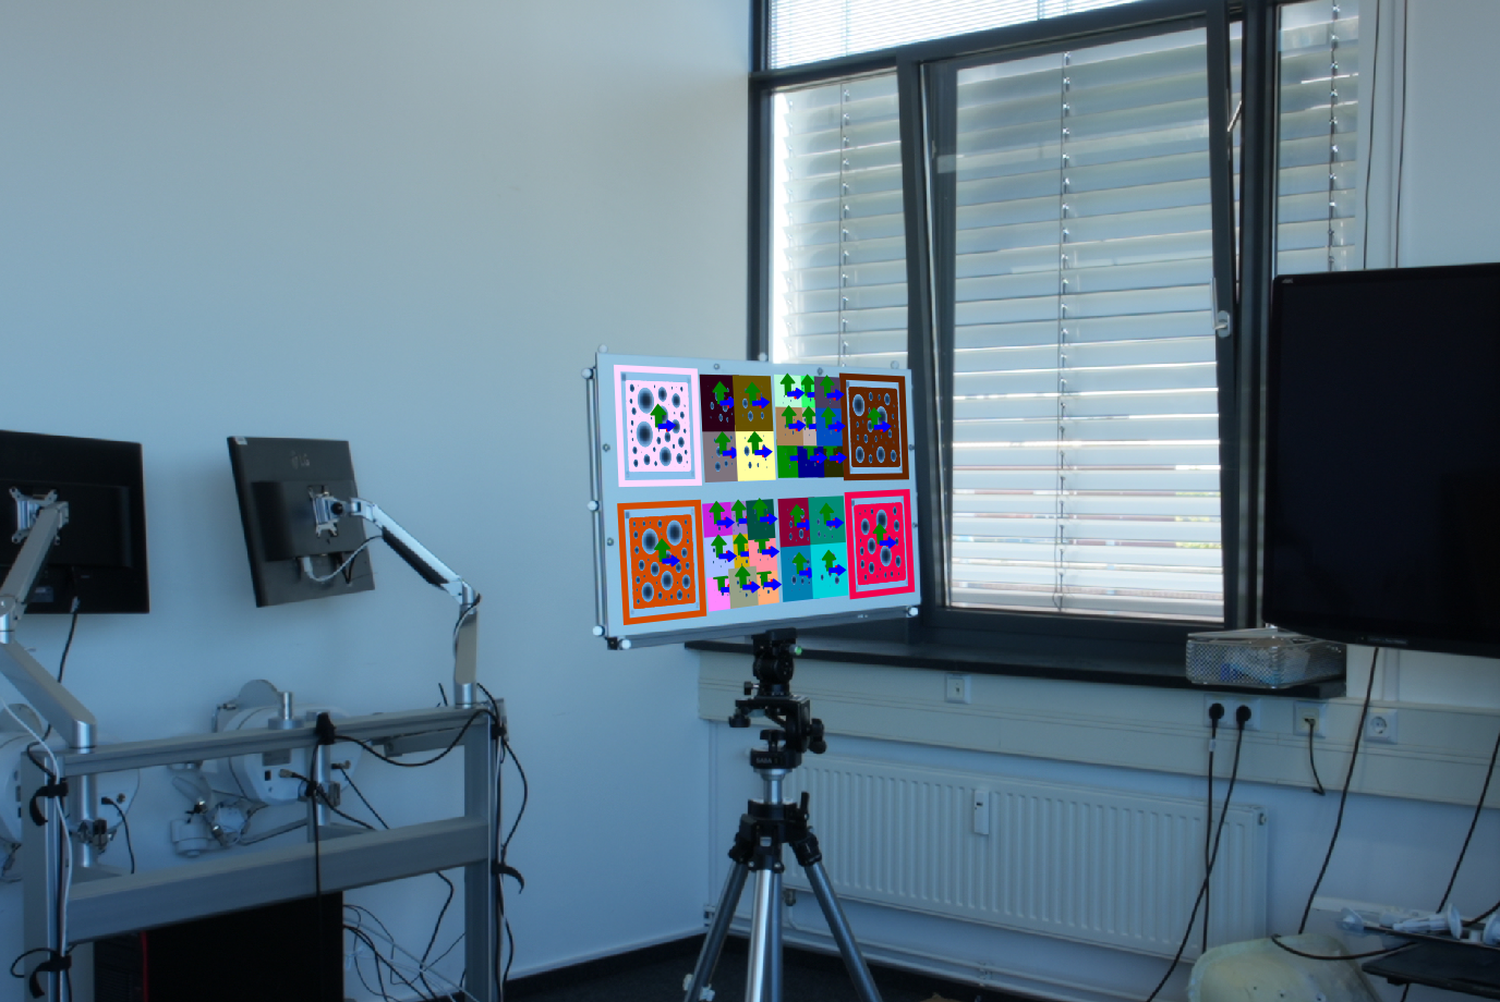
\includegraphics[width=\textwidth]{images/experiment/bb/DSC04563_val.png}
	\end{minipage}\hfill
	\begin{minipage}[c]{0.29\textwidth}
		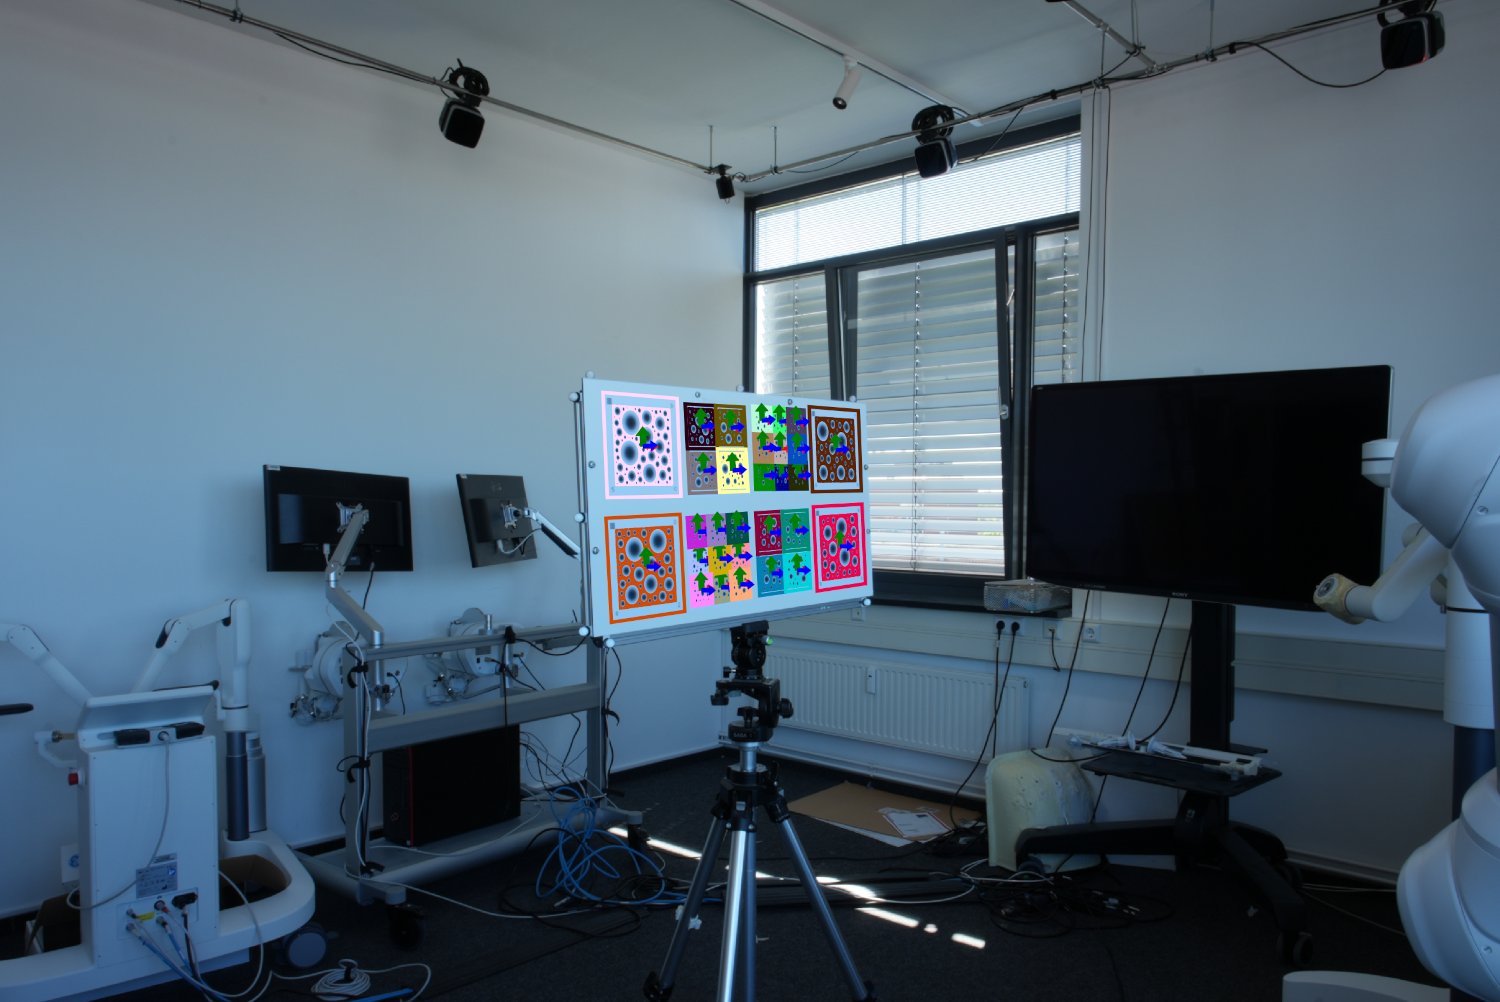
\includegraphics[width=\textwidth]{images/experiment/bb/DSC04544_val.png}
	\end{minipage}\hfill
	\begin{minipage}[c]{0.29\textwidth}
		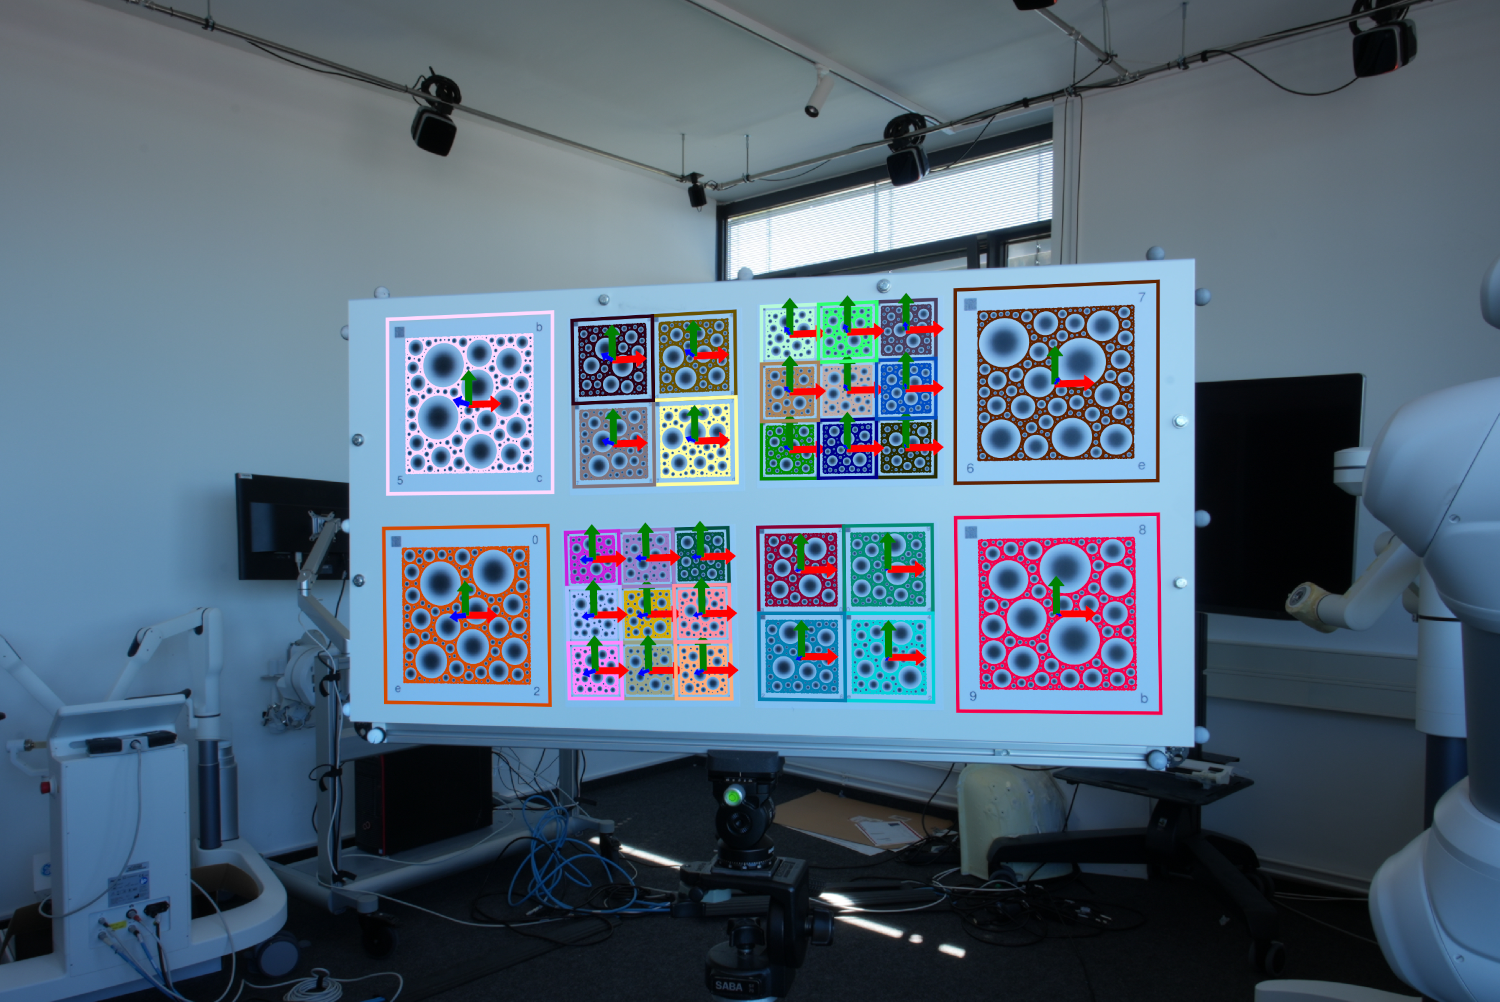
\includegraphics[width=\textwidth]{images/experiment/bb/DSC04530_val.png}
	\end{minipage}

	\vspace{0.4em}

	% Row 2 # april
	\begin{minipage}[c]{0.025\textwidth}
		\centering\rotatebox{90}{\small AprilTag}
	\end{minipage}\hfill
	\begin{minipage}[c]{0.29\textwidth}
		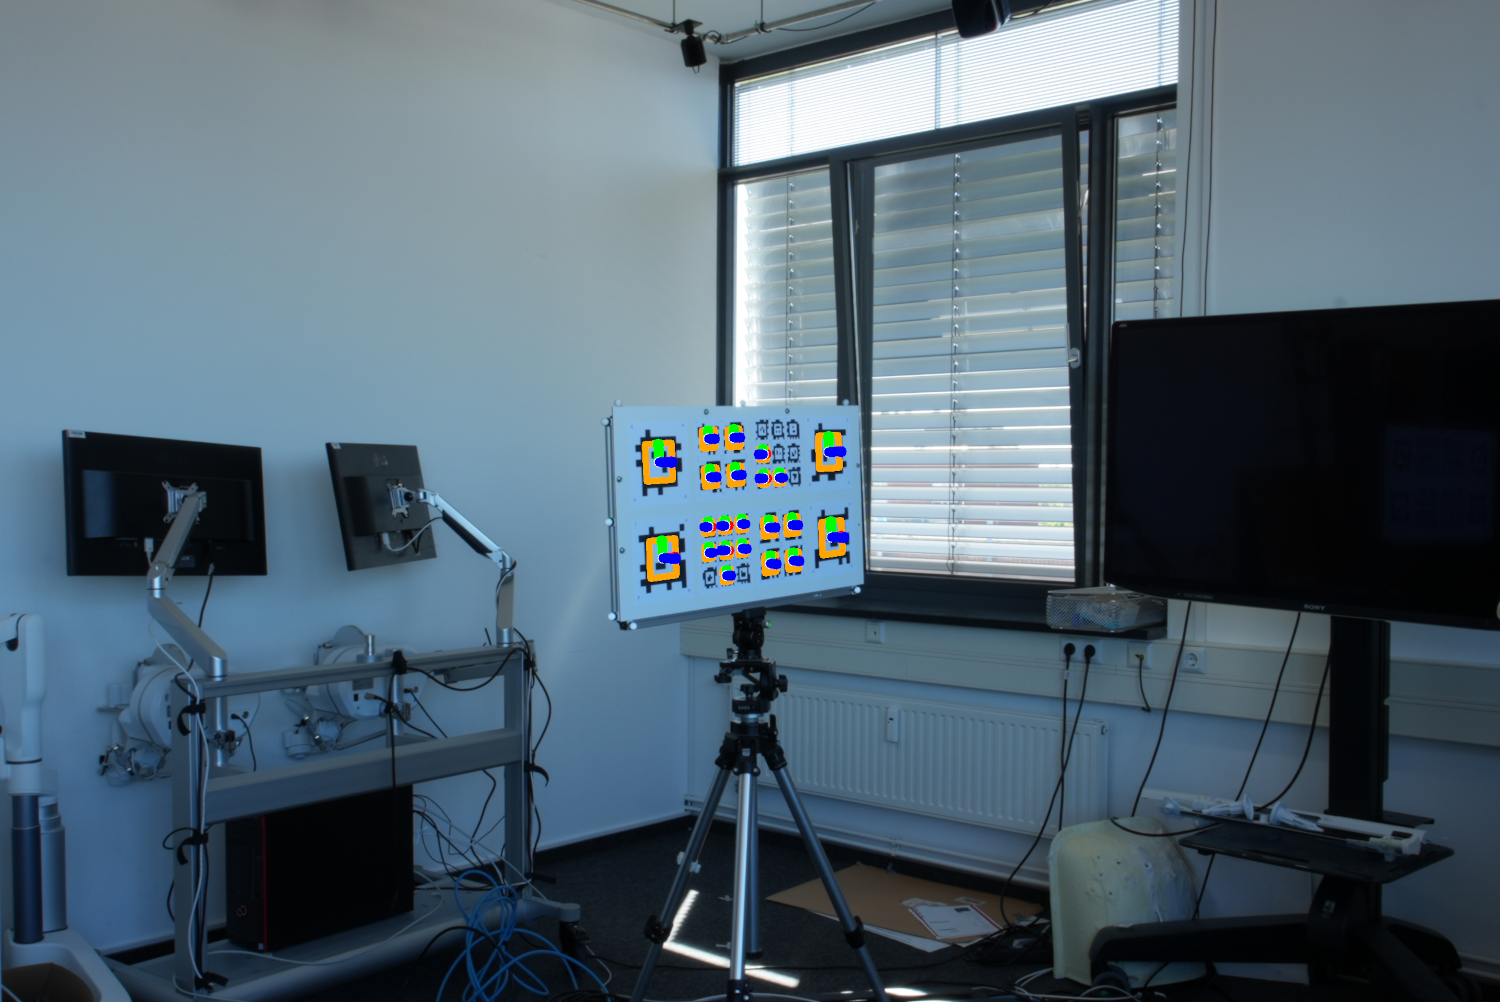
\includegraphics[width=\textwidth]{images/experiment/apr/DSC04465_val.png}
	\end{minipage}\hfill
	\begin{minipage}[c]{0.29\textwidth}
		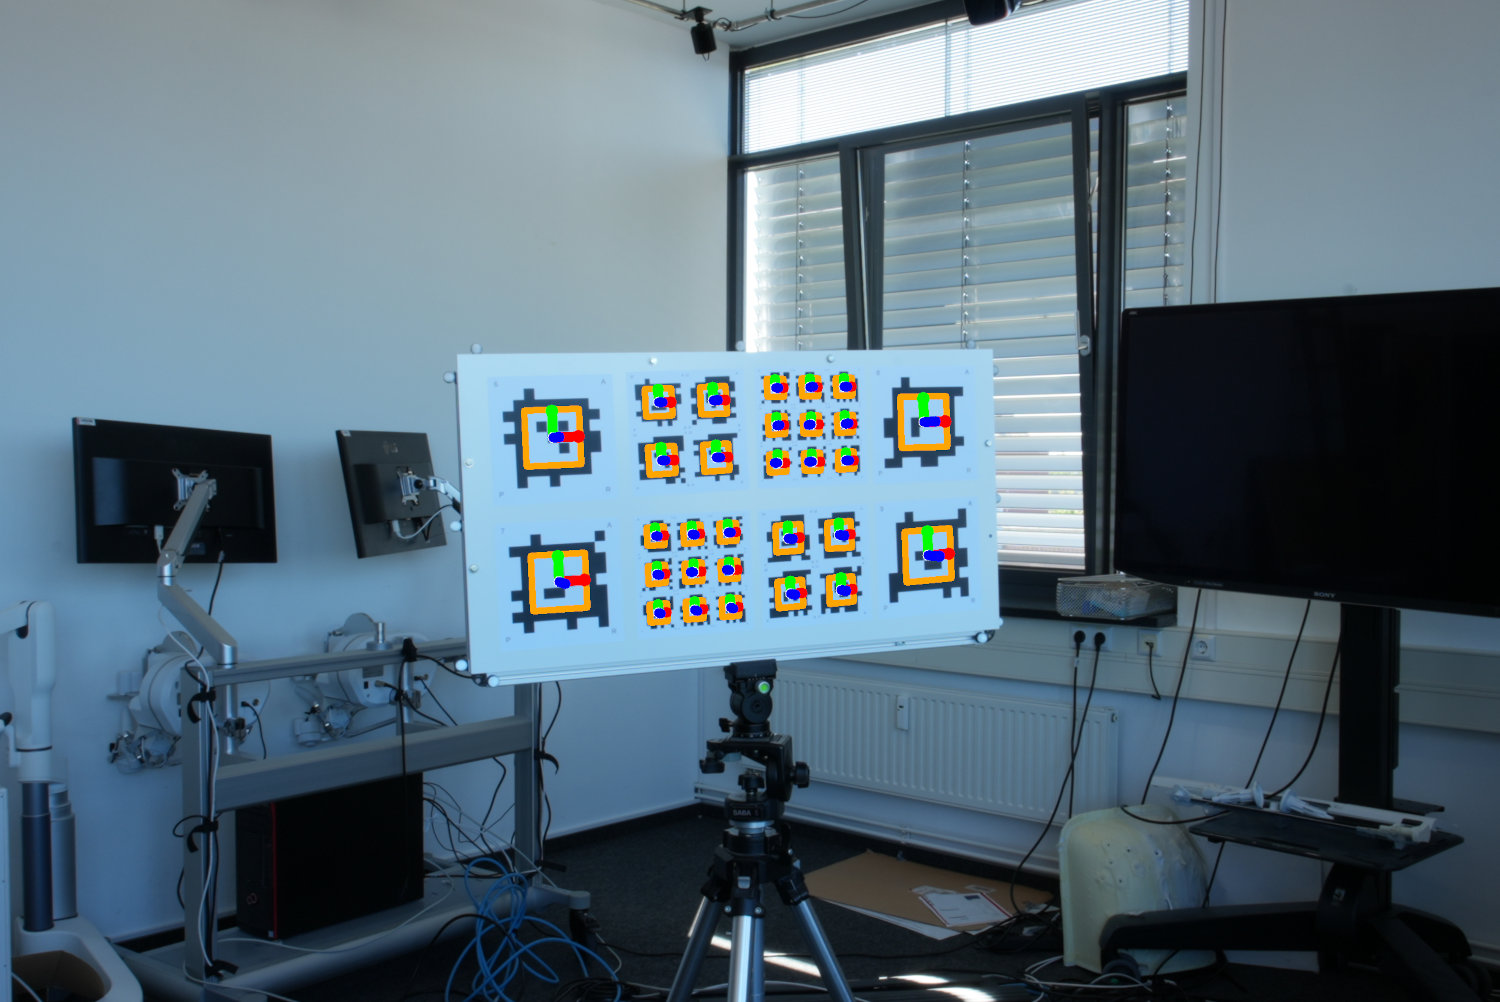
\includegraphics[width=\textwidth]{images/experiment/apr/DSC04443_val.png}
	\end{minipage}\hfill
	\begin{minipage}[c]{0.29\textwidth}
		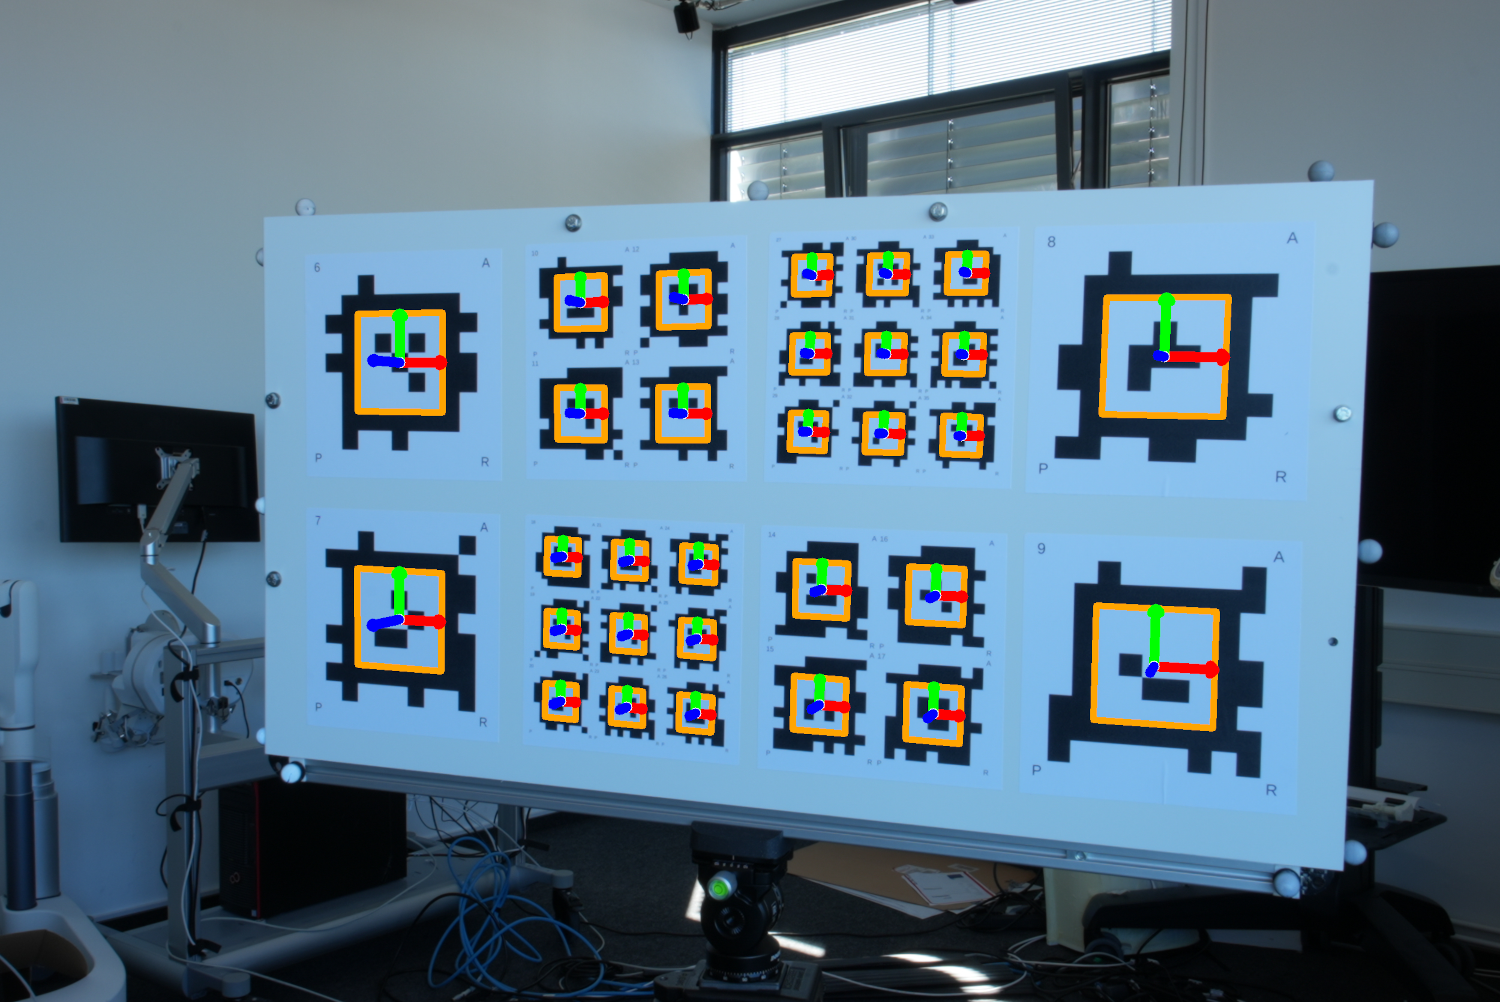
\includegraphics[width=\textwidth]{images/experiment/apr/DSC04433_val.png}
	\end{minipage}

	\vspace{0.4em}

	% Row 3 # aruco
	\begin{minipage}[c]{0.025\textwidth}
		\centering\rotatebox{90}{\small ArUco}
	\end{minipage}\hfill
	\begin{minipage}[c]{0.29\textwidth}
		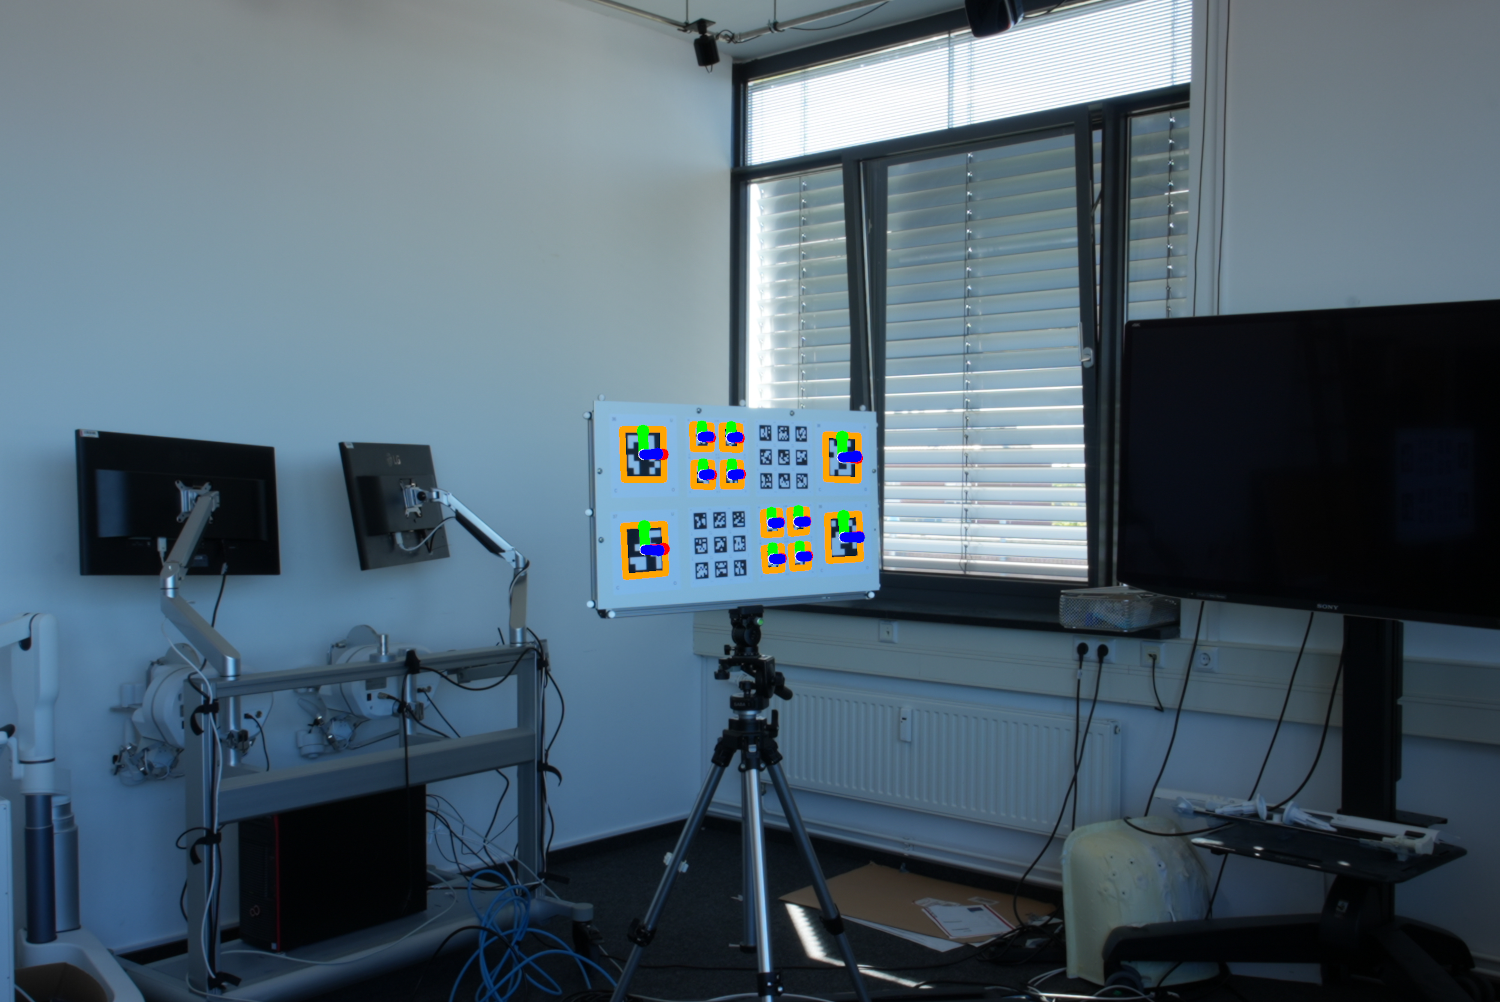
\includegraphics[width=\textwidth]{images/experiment/aru/DSC04375_val.png}
	\end{minipage}\hfill
	\begin{minipage}[c]{0.29\textwidth}
		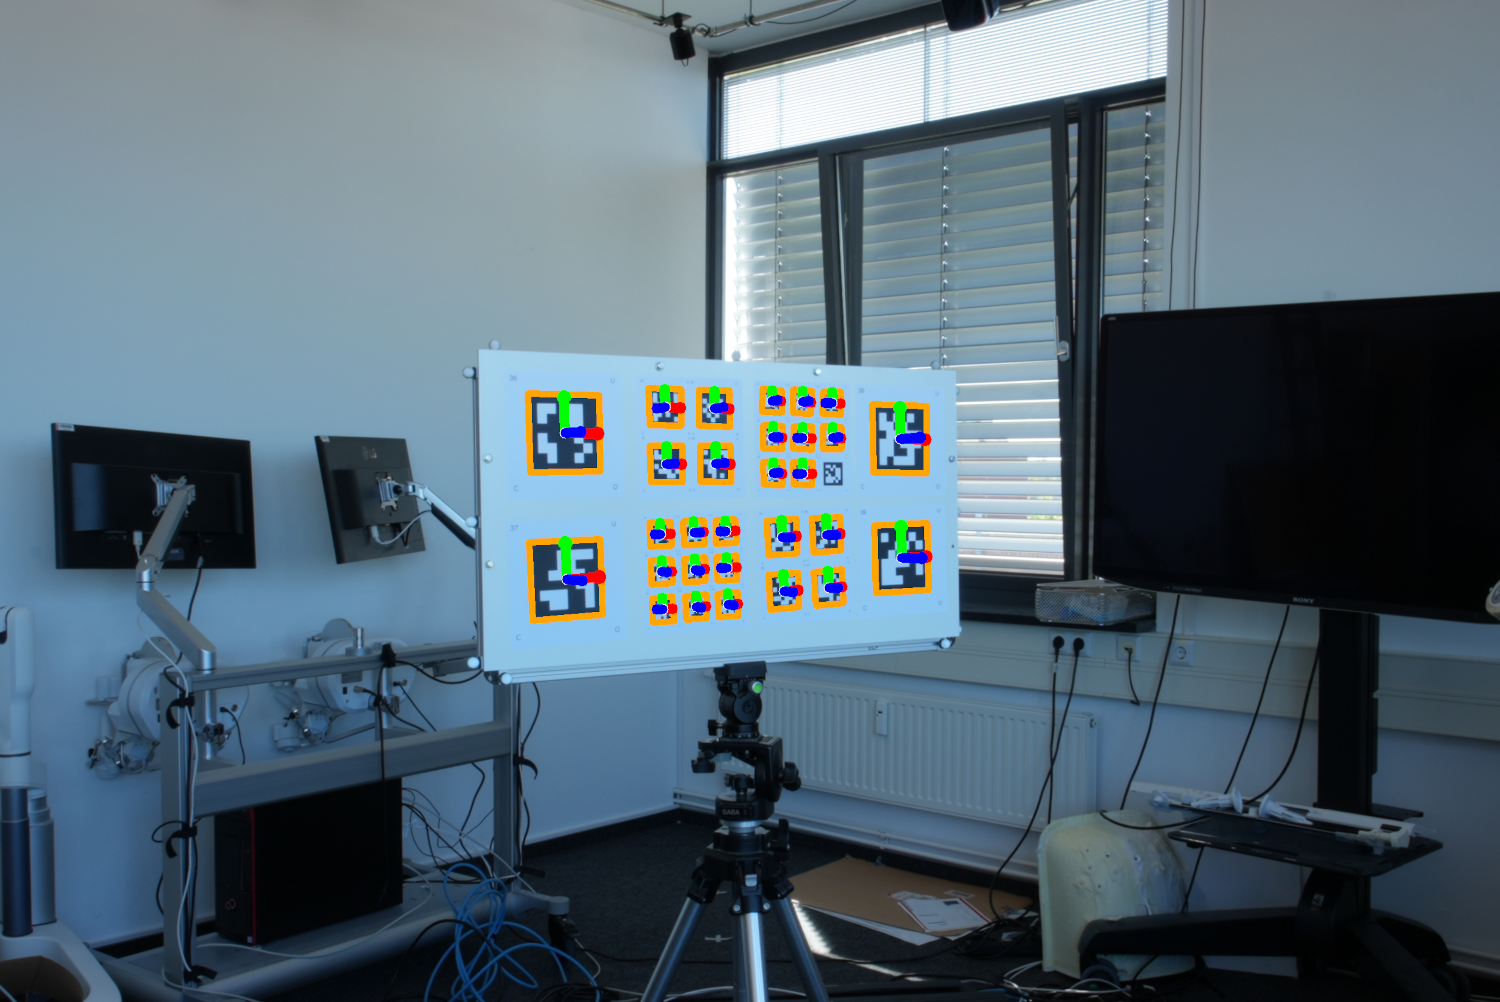
\includegraphics[width=\textwidth]{images/experiment/aru/DSC04355_val.png}
	\end{minipage}\hfill
	\begin{minipage}[c]{0.29\textwidth}
		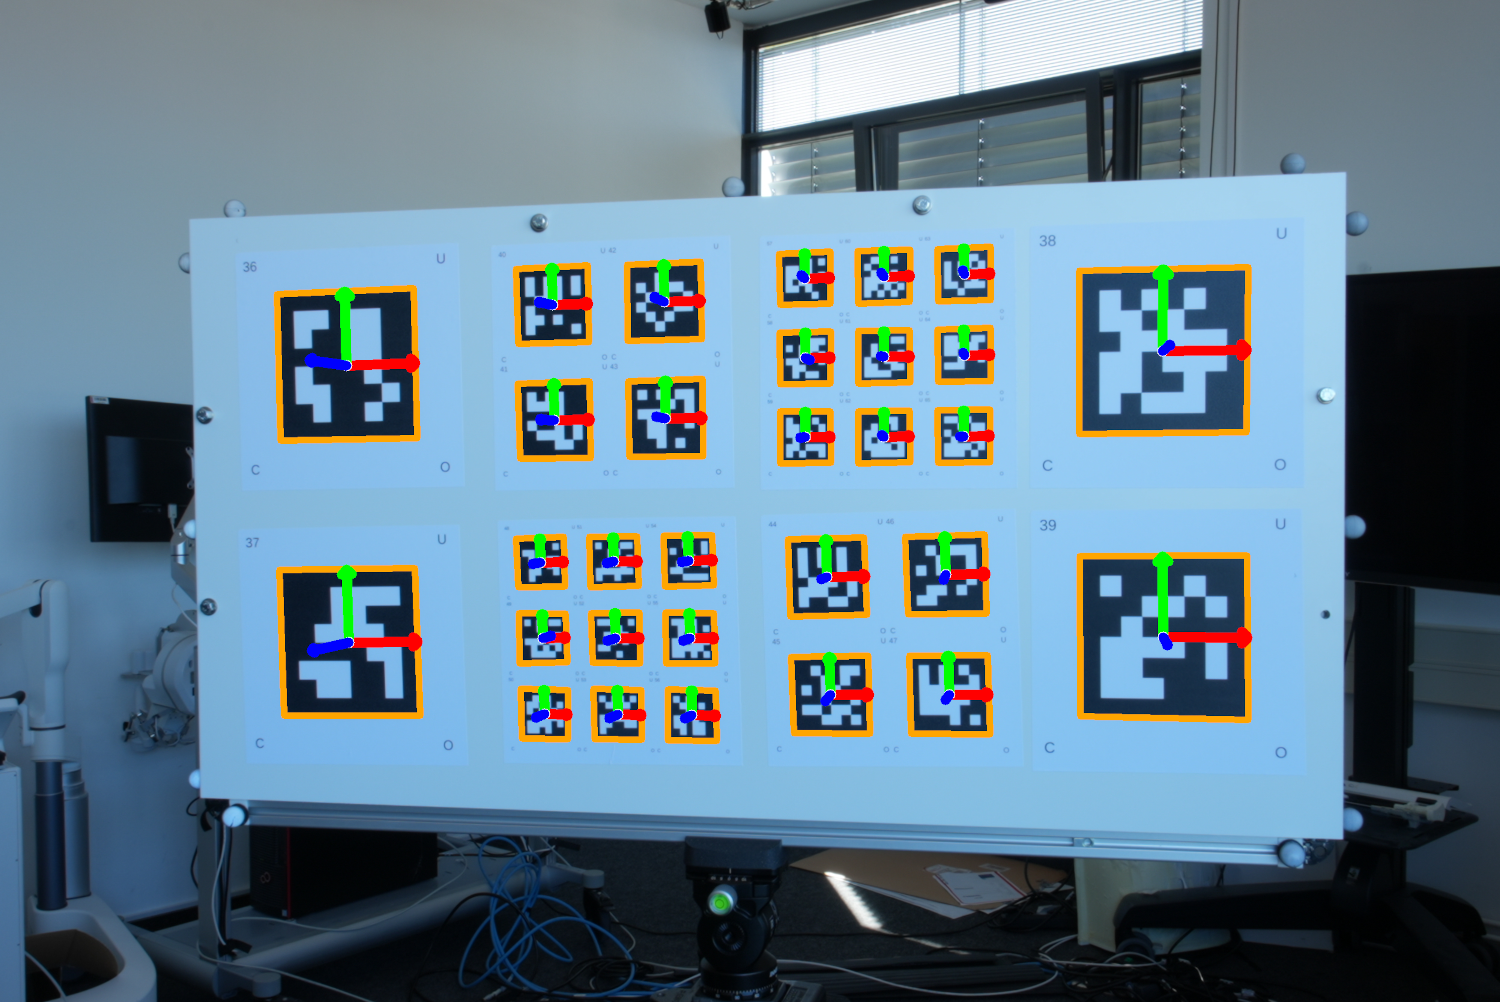
\includegraphics[width=\textwidth]{images/experiment/aru/DSC04343_val.png}
	\end{minipage}

	\vspace{0.4em}

	\caption{Experimental setup. BlobBoards, AprilTag, and ArUco are mounted
		on matched rigid panels containing $\bbGalleryBoards$ markers at three physical
		scales: $\bbBoardsSmall$ small, $\bbBoardsMedium$ medium, and $\bbBoardsLarge$ large. The panel is observed
		at varying distances and obliquities while its $6$-DoF pose is tracked
		by motion capture. Estimated board coordinate frames are overlaid; for
		BlobBoards, the reference pattern is additionally projected under the
		recovered pose.}
	\label{fig:supp:setup}
\end{figure}

\section{Hand--Eye Calibration Diagnostics}
\label{sec:supp:handeye}

\begin{table}[!ht]
	\centering\small
	% handeye_table.tex — generated by scripts/make_handeye_table.jl; do not edit by hand
\begin{tabular}{@{}lrrrr@{}}
\toprule
system & frames & recovered & resid.\ mm & resid.\ deg \\
\midrule
BlobBoards & $41$ & $37$ & $0.68$ & $0.270$ \\
AprilTag & $22$ & $0$ & $2.54$ & $0.432$ \\
ArUco & $15$ & $0$ & $2.81$ & $1.885$ \\
\bottomrule
\end{tabular}

	\caption{Hand--eye calibration diagnostics, one fit per marker system over all $\bbHeMarkers$ boards. \emph{Residual} is the noise scale of the pose residual the staged linear fit reports, in millimetres and degrees; \emph{recovered} counts calibration frames whose untracked camera pose was substituted. The camera is static; its rig was untracked in $\bbHeRecovered$ of the $\bbHeFrames$ BlobBoard calibration frames, which use a substituted constant camera pose admitted only under an explicit constancy gate on the motion-capture reconstruction and the image background.}
	\label{tab:handeye}
\end{table}

\noindent\textbf{Independence of the ground truth.}~ Exactly two observation
streams enter the calibration: the motion-capture rig poses $\mathbf{A}_i$
and the board poses $\hat{\mathbf{B}}_{im}$ reported by the marker system
under test (notation of the main paper). Three properties bound what the
fitted mounts can absorb. First, an explicit calibration set is used,
disjoint from every evaluation frame ($\bbHeFrames$, $\aprHeFrames$ and $\ucoHeFrames$ usable calibration
frames for BlobBoards, AprilTag and ArUco, against $\bbTimeN$, $\aprTimeN$ and $\ucoTimeN$
evaluation frames), so no evaluation frame contributes to the transforms it
is later scored against. Second, the calibration is fitted once per marker
system, from that system's own detections, and then held fixed: every system
is scored against ground truth from its own detector and never a
competitor's, and since the three panels are physically distinct objects a
shared set of mounts does not exist in any case. Third, the fit is heavily
overdetermined and spans the same distances and obliquities as the
evaluation (\cref{sec:supp:derivations}), so a rigid mount can absorb only
an error that is constant over that span. A constant per-system bias is
absorbed for each system alike; scale-, distance- and obliquity-dependent
degradation survives into the numbers the main paper reports. The residual noise scale of the BlobBoard fit is $\bbHeResidTransMM$\,mm and $\bbHeResidRotDeg^\circ$, well below the pose differences the evaluation must resolve (\cref{tab:handeye}).

\section{Hand--Eye Estimator}
\label{sec:supp:derivations}

\noindent\textbf{Conditioning of the fit.}~ The calibration is heavily overdetermined: up to $\bbGalleryBoards$ boards observed in each
of $\ucoHeFrames$--$\bbHeFrames$ calibration frames constrain $6+6\times30$ parameters, and each
board is seen over the same span of distances and obliquities as in the
evaluation. Only a detector error that is constant over that span is
indistinguishable from a rigid mount error and therefore absorbable; any
scale-, distance- or obliquity-dependent component is not.

\noindent\textbf{Staged hand--eye solve.}~ Each of the three stages of the main
paper is in closed form: the shared rotation of $\mathbf{X}$ by Kabsch
alignment of the rotation axes of the relative motions pooled over all
markers, each mount rotation as the chordal mean of its per-frame estimates,
and all translations by one joint least-squares solve. The estimator is
deliberately linear: a pose-residual nonlinear refinement was implemented and
discarded, because it reduced in-sample cost by the amount its own quadratic
model predicts yet extrapolated worse across the evaluation range, the
signature of model misspecification absorbing an unmodelled systematic along a
weakly constrained direction.

\section{Pooled Error Distributions}
\label{sec:supp:pooled}

The main paper breaks recall down by marker size, because that is where the
methods separate. Pooling the three sizes gives the aggregate view below, in
which the tag curves flatten early where the two-fold planar pose ambiguity
takes over.

\begin{figure}[!t]
	\centering
	% error_histograms_table.tex — generated assembly; edit freely
\centering
\begin{tabular}{@{}cc@{}}
% hist_trans.tex — generated (empirical CDFs), edit freely
\providecolor{bbGreen}{HTML}{009E73}
\providecolor{bbBlue}{HTML}{0072B2}
\providecolor{bbOrange}{HTML}{E69F00}
\begin{tikzpicture}[baseline=(current bounding box.center)]
\begin{axis}[width=6.1cm, height=3.9cm, xmode=log, ymin=0, ymax=1,
  xmin=0.5, xmax=400.0, ylabel={$P(\mathrm{error} < x)$},
  xtick={1,10,100}, xticklabels={{1 mm},{10 mm},{100 mm}},
  ytick={0,0.25,0.5,0.75,1}, yticklabels={0,,0.5,,1},
  label style={font=\scriptsize}, tick label style={font=\scriptsize},
  legend style={font=\scriptsize, draw=none, fill=none, at={(0.97,0.06)}, anchor=south east},
  legend cell align=left]
\addplot[forget plot, black!35, dashed, line width=0.5pt] coordinates {(0.5,0.5) (400.0,0.5)};
\addplot[const plot, draw=bbBlue, line width=1.0pt] coordinates {(0.5,0) (0.50005,0.0005952) (0.57697,0.003571) (0.72183,0.006548) (1.0047,0.009524) (1.1181,0.0125) (1.2068,0.01548) (1.3329,0.01845) (1.424,0.02143) (1.4768,0.0244) (1.565,0.02738) (1.6257,0.03036) (1.6758,0.03333) (1.7068,0.03631) (1.7296,0.03929) (1.7572,0.04226) (1.8002,0.04524) (1.8305,0.04821) (1.8593,0.05119) (1.8759,0.05417) (1.9029,0.05714) (1.9327,0.06012) (1.956,0.0631) (1.9805,0.06607) (2.0277,0.06905) (2.0427,0.07202) (2.0665,0.075) (2.0895,0.07798) (2.113,0.08095) (2.1351,0.08393) (2.1445,0.0869) (2.1673,0.08988) (2.1746,0.09286) (2.2048,0.09583) (2.2148,0.09881) (2.2444,0.1018) (2.2529,0.1048) (2.2668,0.1077) (2.298,0.1107) (2.3107,0.1137) (2.3231,0.1167) (2.3522,0.1196) (2.3683,0.1226) (2.3765,0.1256) (2.3961,0.1286) (2.4318,0.1315) (2.4531,0.1345) (2.4616,0.1375) (2.4716,0.1405) (2.4899,0.1435) (2.5012,0.1464) (2.5116,0.1494) (2.526,0.1524) (2.5565,0.1554) (2.5632,0.1583) (2.5725,0.1613) (2.5888,0.1643) (2.6081,0.1673) (2.6154,0.1702) (2.63,0.1732) (2.6629,0.1762) (2.6822,0.1792) (2.6976,0.1821) (2.713,0.1851) (2.7229,0.1881) (2.7336,0.1911) (2.7526,0.194) (2.7679,0.197) (2.8041,0.2) (2.8199,0.203) (2.8322,0.206) (2.8382,0.2089) (2.8525,0.2119) (2.8569,0.2149) (2.8624,0.2179) (2.8882,0.2208) (2.9077,0.2238) (2.9136,0.2268) (2.9233,0.2298) (2.9308,0.2327) (2.9371,0.2357) (2.9526,0.2387) (2.9836,0.2417) (3.0052,0.2446) (3.0243,0.2476) (3.0325,0.2506) (3.0402,0.2536) (3.0586,0.2565) (3.07,0.2595) (3.0886,0.2625) (3.1004,0.2655) (3.1196,0.2685) (3.1427,0.2714) (3.1568,0.2744) (3.1667,0.2774) (3.1855,0.2804) (3.1944,0.2833) (3.2089,0.2863) (3.22,0.2893) (3.2261,0.2923) (3.2479,0.2952) (3.2538,0.2982) (3.2731,0.3012) (3.2865,0.3042) (3.298,0.3071) (3.3078,0.3101) (3.3242,0.3131) (3.3266,0.3161) (3.3384,0.319) (3.3514,0.322) (3.3669,0.325) (3.3919,0.328) (3.4012,0.331) (3.4172,0.3339) (3.4282,0.3369) (3.4413,0.3399) (3.472,0.3429) (3.4899,0.3458) (3.505,0.3488) (3.5295,0.3518) (3.5371,0.3548) (3.5525,0.3577) (3.5644,0.3607) (3.5806,0.3637) (3.5955,0.3667) (3.5989,0.3696) (3.6128,0.3726) (3.6292,0.3756) (3.6448,0.3786) (3.6575,0.3815) (3.6656,0.3845) (3.6772,0.3875) (3.6987,0.3905) (3.7164,0.3935) (3.7298,0.3964) (3.7523,0.3994) (3.7628,0.4024) (3.7847,0.4054) (3.8041,0.4083) (3.8206,0.4113) (3.8301,0.4143) (3.838,0.4173) (3.8444,0.4202) (3.8578,0.4232) (3.9014,0.4262) (3.9242,0.4292) (3.9417,0.4321) (3.957,0.4351) (3.9901,0.4381) (4.0144,0.4411) (4.038,0.444) (4.0577,0.447) (4.0761,0.45) (4.0979,0.453) (4.1365,0.456) (4.1591,0.4589) (4.1777,0.4619) (4.2025,0.4649) (4.2287,0.4679) (4.265,0.4708) (4.2824,0.4738) (4.3129,0.4768) (4.3468,0.4798) (4.366,0.4827) (4.398,0.4857) (4.4285,0.4887) (4.4724,0.4917) (4.4898,0.4946) (4.5209,0.4976) (4.5434,0.5006) (4.5602,0.5036) (4.5883,0.5065) (4.6002,0.5095) (4.6336,0.5125) (4.6432,0.5155) (4.6569,0.5185) (4.6802,0.5214) (4.6982,0.5244) (4.7138,0.5274) (4.7378,0.5304) (4.748,0.5333) (4.7666,0.5363) (4.7952,0.5393) (4.8168,0.5423) (4.871,0.5452) (4.8998,0.5482) (4.9198,0.5512) (4.9685,0.5542) (4.9908,0.5571) (5.0191,0.5601) (5.0284,0.5631) (5.0563,0.5661) (5.1404,0.569) (5.1919,0.572) (5.2108,0.575) (5.2537,0.578) (5.2848,0.581) (5.3072,0.5839) (5.3248,0.5869) (5.3871,0.5899) (5.4041,0.5929) (5.4307,0.5958) (5.4525,0.5988) (5.4912,0.6018) (5.5207,0.6048) (5.5735,0.6077) (5.6159,0.6107) (5.638,0.6137) (5.7092,0.6167) (5.7496,0.6196) (5.796,0.6226) (5.8657,0.6256) (5.9469,0.6286) (5.9634,0.6315) (6.0112,0.6345) (6.0436,0.6375) (6.0752,0.6405) (6.1924,0.6435) (6.2339,0.6464) (6.3011,0.6494) (6.3556,0.6524) (6.4483,0.6554) (6.4936,0.6583) (6.5183,0.6613) (6.6356,0.6643) (6.6929,0.6673) (6.7408,0.6702) (6.8103,0.6732) (6.864,0.6762) (7.0054,0.6792) (7.054,0.6821) (7.1112,0.6851) (7.1629,0.6881) (7.2999,0.6911) (7.3436,0.694) (7.4318,0.697) (7.4805,0.7) (7.5587,0.703) (7.6848,0.706) (7.7215,0.7089) (7.7857,0.7119) (7.8873,0.7149) (8.0128,0.7179) (8.1136,0.7208) (8.1817,0.7238) (8.2514,0.7268) (8.3562,0.7298) (8.5491,0.7327) (8.6019,0.7357) (8.7783,0.7387) (8.9325,0.7417) (9.1057,0.7446) (9.3234,0.7476) (9.4329,0.7506) (9.5004,0.7536) (9.6267,0.7565) (9.8321,0.7595) (10.129,0.7625) (10.511,0.7655) (10.639,0.7685) (10.982,0.7714) (11.379,0.7744) (11.573,0.7774) (12.063,0.7804) (12.776,0.7833) (13.18,0.7863) (14.053,0.7893) (14.413,0.7923) (16.325,0.7952) (19.615,0.7982) (24.183,0.8012) (400.0,0.8012)};
\addlegendentry{BlobBoards}
\addplot[const plot, draw=bbOrange, line width=1.0pt] coordinates {(0.5,0) (0.50005,0.0005848) (1.1913,0.002924) (1.6583,0.005263) (1.7461,0.007602) (2.1329,0.009942) (2.1842,0.01228) (2.4399,0.01462) (2.4853,0.01696) (2.599,0.0193) (2.7823,0.02164) (2.9157,0.02398) (3.0282,0.02632) (3.1084,0.02865) (3.2207,0.03099) (3.2999,0.03333) (3.3496,0.03567) (3.426,0.03801) (3.5068,0.04035) (3.6273,0.04269) (3.6793,0.04503) (3.7387,0.04737) (3.7783,0.04971) (3.8544,0.05205) (3.9423,0.05439) (4.0194,0.05673) (4.0477,0.05906) (4.0941,0.0614) (4.2277,0.06374) (4.3097,0.06608) (4.3528,0.06842) (4.4401,0.07076) (4.5276,0.0731) (4.6054,0.07544) (4.7489,0.07778) (4.8088,0.08012) (4.9312,0.08246) (5.0061,0.0848) (5.1678,0.08713) (5.1995,0.08947) (5.2196,0.09181) (5.3377,0.09415) (5.3735,0.09649) (5.4329,0.09883) (5.4745,0.1012) (5.5031,0.1035) (5.5471,0.1058) (5.6042,0.1082) (5.616,0.1105) (5.6761,0.1129) (5.6956,0.1152) (5.7996,0.1175) (5.8191,0.1199) (5.8596,0.1222) (5.897,0.1246) (5.9467,0.1269) (5.9832,0.1292) (6.0193,0.1316) (6.0688,0.1339) (6.1301,0.1363) (6.1809,0.1386) (6.1952,0.1409) (6.2347,0.1433) (6.3231,0.1456) (6.3492,0.148) (6.3667,0.1503) (6.4242,0.1526) (6.4316,0.155) (6.4678,0.1573) (6.5025,0.1596) (6.523,0.162) (6.5542,0.1643) (6.5879,0.1667) (6.6316,0.169) (6.6682,0.1713) (6.6906,0.1737) (6.757,0.176) (6.8345,0.1784) (6.855,0.1807) (6.8796,0.183) (6.9403,0.1854) (6.9791,0.1877) (6.9989,0.1901) (7.0687,0.1924) (7.087,0.1947) (7.114,0.1971) (7.17,0.1994) (7.2141,0.2018) (7.2219,0.2041) (7.2876,0.2064) (7.3132,0.2088) (7.3329,0.2111) (7.3908,0.2135) (7.4635,0.2158) (7.5704,0.2181) (7.6114,0.2205) (7.6308,0.2228) (7.6438,0.2251) (7.7114,0.2275) (7.7268,0.2298) (7.7727,0.2322) (7.8687,0.2345) (7.9019,0.2368) (7.9919,0.2392) (8.0538,0.2415) (8.1244,0.2439) (8.2412,0.2462) (8.2733,0.2485) (8.3459,0.2509) (8.4681,0.2532) (8.6198,0.2556) (8.828,0.2579) (8.9365,0.2602) (8.9533,0.2626) (9.0667,0.2649) (9.1691,0.2673) (9.4122,0.2696) (9.675,0.2719) (10.028,0.2743) (10.625,0.2766) (10.759,0.2789) (11.245,0.2813) (11.995,0.2836) (12.504,0.286) (12.881,0.2883) (13.59,0.2906) (14.014,0.293) (14.483,0.2953) (14.873,0.2977) (15.492,0.3) (15.97,0.3023) (16.517,0.3047) (16.755,0.307) (17.206,0.3094) (17.597,0.3117) (17.82,0.314) (18.323,0.3164) (18.587,0.3187) (19.077,0.3211) (19.316,0.3234) (19.86,0.3257) (19.993,0.3281) (20.546,0.3304) (20.834,0.3327) (21.182,0.3351) (21.455,0.3374) (21.804,0.3398) (21.981,0.3421) (22.106,0.3444) (22.679,0.3468) (23.251,0.3491) (24.022,0.3515) (24.37,0.3538) (24.863,0.3561) (25.012,0.3585) (25.27,0.3608) (25.437,0.3632) (25.865,0.3655) (26.048,0.3678) (26.128,0.3702) (26.356,0.3725) (26.751,0.3749) (26.937,0.3772) (27.608,0.3795) (28.156,0.3819) (28.667,0.3842) (28.985,0.3865) (29.292,0.3889) (29.604,0.3912) (29.758,0.3936) (30.201,0.3959) (30.345,0.3982) (30.577,0.4006) (30.629,0.4029) (31.009,0.4053) (31.188,0.4076) (31.582,0.4099) (31.886,0.4123) (32.025,0.4146) (32.339,0.417) (32.655,0.4193) (32.913,0.4216) (33.059,0.424) (33.291,0.4263) (33.553,0.4287) (33.85,0.431) (34.063,0.4333) (34.27,0.4357) (34.628,0.438) (34.958,0.4404) (35.073,0.4427) (35.367,0.445) (35.66,0.4474) (35.777,0.4497) (35.959,0.452) (36.276,0.4544) (36.481,0.4567) (36.61,0.4591) (36.89,0.4614) (37.286,0.4637) (37.418,0.4661) (37.57,0.4684) (37.613,0.4708) (37.973,0.4731) (38.244,0.4754) (38.409,0.4778) (38.724,0.4801) (38.939,0.4825) (39.035,0.4848) (39.169,0.4871) (39.222,0.4895) (39.892,0.4918) (40.276,0.4942) (40.649,0.4965) (40.767,0.4988) (40.918,0.5012) (41.056,0.5035) (41.104,0.5058) (41.313,0.5082) (41.587,0.5105) (41.925,0.5129) (42.276,0.5152) (42.457,0.5175) (42.849,0.5199) (43.124,0.5222) (43.259,0.5246) (43.549,0.5269) (43.745,0.5292) (44.135,0.5316) (44.334,0.5339) (44.804,0.5363) (45.547,0.5386) (45.709,0.5409) (45.996,0.5433) (46.846,0.5456) (47.116,0.548) (47.357,0.5503) (47.699,0.5526) (48.036,0.555) (48.363,0.5573) (48.852,0.5596) (49.149,0.562) (49.48,0.5643) (50.054,0.5667) (50.286,0.569) (50.624,0.5713) (50.95,0.5737) (51.508,0.576) (52.169,0.5784) (52.744,0.5807) (53.572,0.583) (54.312,0.5854) (54.781,0.5877) (55.067,0.5901) (55.35,0.5924) (55.66,0.5947) (57.035,0.5971) (57.607,0.5994) (58.444,0.6018) (58.877,0.6041) (59.167,0.6064) (59.929,0.6088) (60.838,0.6111) (62.282,0.6135) (63.191,0.6158) (64.192,0.6181) (65.445,0.6205) (66.287,0.6228) (66.807,0.6251) (67.741,0.6275) (68.306,0.6298) (68.468,0.6322) (68.825,0.6345) (69.624,0.6368) (70.601,0.6392) (70.957,0.6415) (71.528,0.6439) (72.065,0.6462) (73.227,0.6485) (73.411,0.6509) (74.236,0.6532) (75.49,0.6556) (76.504,0.6579) (77.174,0.6602) (77.864,0.6626) (78.263,0.6649) (78.565,0.6673) (79.193,0.6696) (80.633,0.6719) (81.412,0.6743) (81.83,0.6766) (82.485,0.6789) (82.822,0.6813) (84.366,0.6836) (84.745,0.686) (85.503,0.6883) (85.818,0.6906) (87.03,0.693) (87.975,0.6953) (88.969,0.6977) (89.886,0.7) (90.35,0.7023) (90.942,0.7047) (91.927,0.707) (94.114,0.7094) (95.899,0.7117) (96.635,0.714) (99.302,0.7164) (102.19,0.7187) (106.7,0.7211) (108.61,0.7234) (112.46,0.7257) (122.85,0.7281) (400.0,0.7281)};
\addlegendentry{AprilTag}
\addplot[const plot, draw=bbGreen, line width=1.0pt] coordinates {(0.5,0) (1.6435,0.0005848) (2.6268,0.002339) (3.039,0.004094) (3.2166,0.005848) (3.4328,0.007602) (3.7963,0.009357) (3.9519,0.01111) (4.113,0.01287) (4.2231,0.01462) (4.2869,0.01637) (4.3482,0.01813) (4.4128,0.01988) (4.5522,0.02164) (4.7124,0.02339) (4.8355,0.02515) (4.9476,0.0269) (5.0025,0.02865) (5.0344,0.03041) (5.0877,0.03216) (5.1369,0.03392) (5.1781,0.03567) (5.2209,0.03743) (5.322,0.03918) (5.486,0.04094) (5.5079,0.04269) (5.5738,0.04444) (5.6256,0.0462) (5.6499,0.04795) (5.7042,0.04971) (5.7468,0.05146) (5.8026,0.05322) (5.8187,0.05497) (5.9327,0.05673) (6.0166,0.05848) (6.0925,0.06023) (6.1333,0.06199) (6.1728,0.06374) (6.2288,0.0655) (6.2547,0.06725) (6.3057,0.06901) (6.3582,0.07076) (6.3872,0.07251) (6.4843,0.07427) (6.4986,0.07602) (6.5695,0.07778) (6.6837,0.07953) (6.7423,0.08129) (6.7624,0.08304) (6.8023,0.0848) (6.8204,0.08655) (6.8413,0.0883) (6.8583,0.09006) (6.8986,0.09181) (6.9745,0.09357) (7.073,0.09532) (7.1945,0.09708) (7.2395,0.09883) (7.2835,0.1006) (7.2973,0.1023) (7.3373,0.1041) (7.3617,0.1058) (7.3799,0.1076) (7.4054,0.1094) (7.4799,0.1111) (7.5101,0.1129) (7.5411,0.1146) (7.5561,0.1164) (7.6196,0.1181) (7.6561,0.1199) (7.699,0.1216) (7.8067,0.1234) (7.8577,0.1251) (7.8843,0.1269) (7.9473,0.1287) (7.9636,0.1304) (8.0755,0.1322) (8.144,0.1339) (8.1854,0.1357) (8.2762,0.1374) (8.2979,0.1392) (8.3269,0.1409) (8.407,0.1427) (8.4639,0.1444) (8.5075,0.1462) (8.5342,0.148) (8.5906,0.1497) (8.6213,0.1515) (8.7267,0.1532) (8.7948,0.155) (8.8613,0.1567) (8.9103,0.1585) (8.9303,0.1602) (8.9903,0.162) (9.0117,0.1637) (9.0939,0.1655) (9.1729,0.1673) (9.1885,0.169) (9.2219,0.1708) (9.255,0.1725) (9.2927,0.1743) (9.3813,0.176) (9.3948,0.1778) (9.4903,0.1795) (9.55,0.1813) (9.6411,0.183) (9.868,0.1848) (9.9635,0.1865) (10.0,0.1883) (10.022,0.1901) (10.101,0.1918) (10.127,0.1936) (10.166,0.1953) (10.248,0.1971) (10.294,0.1988) (10.381,0.2006) (10.427,0.2023) (10.457,0.2041) (10.55,0.2058) (10.644,0.2076) (10.793,0.2094) (10.817,0.2111) (10.864,0.2129) (10.914,0.2146) (10.966,0.2164) (11.008,0.2181) (11.042,0.2199) (11.129,0.2216) (11.188,0.2234) (11.211,0.2251) (11.27,0.2269) (11.321,0.2287) (11.434,0.2304) (11.571,0.2322) (11.645,0.2339) (11.811,0.2357) (11.95,0.2374) (12.005,0.2392) (12.121,0.2409) (12.186,0.2427) (12.446,0.2444) (12.495,0.2462) (12.66,0.248) (12.897,0.2497) (13.136,0.2515) (13.46,0.2532) (13.634,0.255) (13.755,0.2567) (13.967,0.2585) (14.053,0.2602) (14.111,0.262) (14.523,0.2637) (14.712,0.2655) (15.165,0.2673) (15.269,0.269) (15.794,0.2708) (15.95,0.2725) (16.585,0.2743) (16.907,0.276) (17.033,0.2778) (17.613,0.2795) (17.878,0.2813) (18.455,0.283) (19.045,0.2848) (19.546,0.2865) (19.82,0.2883) (21.178,0.2901) (22.069,0.2918) (22.653,0.2936) (22.846,0.2953) (23.18,0.2971) (23.686,0.2988) (24.287,0.3006) (24.417,0.3023) (25.141,0.3041) (25.459,0.3058) (25.917,0.3076) (26.498,0.3094) (26.673,0.3111) (26.76,0.3129) (27.064,0.3146) (27.27,0.3164) (27.513,0.3181) (28.016,0.3199) (28.563,0.3216) (28.642,0.3234) (28.936,0.3251) (29.057,0.3269) (29.292,0.3287) (29.953,0.3304) (30.354,0.3322) (30.841,0.3339) (31.411,0.3357) (31.688,0.3374) (32.14,0.3392) (32.332,0.3409) (33.077,0.3427) (33.354,0.3444) (33.8,0.3462) (34.135,0.348) (34.323,0.3497) (34.976,0.3515) (35.311,0.3532) (35.549,0.355) (35.907,0.3567) (35.989,0.3585) (36.303,0.3602) (36.499,0.362) (36.65,0.3637) (37.172,0.3655) (37.442,0.3673) (37.811,0.369) (38.058,0.3708) (38.48,0.3725) (38.659,0.3743) (38.939,0.376) (39.372,0.3778) (39.876,0.3795) (40.219,0.3813) (40.265,0.383) (40.44,0.3848) (40.764,0.3865) (40.823,0.3883) (41.108,0.3901) (41.574,0.3918) (42.223,0.3936) (42.331,0.3953) (42.397,0.3971) (42.559,0.3988) (42.825,0.4006) (43.014,0.4023) (43.407,0.4041) (44.026,0.4058) (44.413,0.4076) (44.793,0.4094) (45.162,0.4111) (45.608,0.4129) (46.135,0.4146) (46.567,0.4164) (46.774,0.4181) (47.104,0.4199) (47.311,0.4216) (47.557,0.4234) (48.092,0.4251) (48.189,0.4269) (48.364,0.4287) (49.041,0.4304) (49.294,0.4322) (49.629,0.4339) (49.822,0.4357) (49.939,0.4374) (50.336,0.4392) (50.725,0.4409) (51.664,0.4427) (52.092,0.4444) (52.504,0.4462) (52.944,0.448) (53.265,0.4497) (53.441,0.4515) (53.626,0.4532) (54.017,0.455) (54.907,0.4567) (55.16,0.4585) (55.456,0.4602) (56.071,0.462) (56.34,0.4637) (56.783,0.4655) (57.187,0.4673) (57.532,0.469) (57.729,0.4708) (57.953,0.4725) (58.534,0.4743) (59.25,0.476) (59.645,0.4778) (60.309,0.4795) (60.8,0.4813) (61.412,0.483) (61.528,0.4848) (61.723,0.4865) (62.341,0.4883) (62.813,0.4901) (63.36,0.4918) (63.814,0.4936) (64.073,0.4953) (64.813,0.4971) (65.008,0.4988) (65.384,0.5006) (66.493,0.5023) (67.109,0.5041) (67.859,0.5058) (68.405,0.5076) (69.299,0.5094) (69.656,0.5111) (70.052,0.5129) (70.696,0.5146) (70.918,0.5164) (72.363,0.5181) (72.709,0.5199) (73.564,0.5216) (73.671,0.5234) (73.912,0.5251) (74.435,0.5269) (75.84,0.5287) (76.924,0.5304) (78.385,0.5322) (78.575,0.5339) (80.108,0.5357) (82.349,0.5374) (83.309,0.5392) (84.021,0.5409) (87.019,0.5427) (88.909,0.5444) (92.835,0.5462) (94.703,0.548) (96.134,0.5497) (97.543,0.5515) (99.688,0.5532) (104.47,0.555) (107.34,0.5567) (111.35,0.5585) (112.96,0.5602) (117.47,0.562) (122.76,0.5637) (128.94,0.5655) (134.4,0.5673) (159.47,0.569) (400.0,0.569)};
\addlegendentry{ArUco}
\end{axis}
\end{tikzpicture}
 & % hist_rot.tex — generated (empirical CDFs), edit freely
\providecolor{bbGreen}{HTML}{009E73}
\providecolor{bbBlue}{HTML}{0072B2}
\providecolor{bbOrange}{HTML}{E69F00}
\begin{tikzpicture}[baseline=(current bounding box.center)]
\begin{axis}[width=6.1cm, height=3.9cm, xmode=log, ymin=0, ymax=1,
  xmin=0.02, xmax=200.0, ylabel={$P(\mathrm{error} < x)$},
  xtick={0.1,1,10,100}, xticklabels={{0.1$^\circ$},{1$^\circ$},{10$^\circ$},{100$^\circ$}},
  ytick={0,0.25,0.5,0.75,1}, yticklabels={0,,0.5,,1},
  label style={font=\scriptsize}, tick label style={font=\scriptsize},
  legend style={font=\scriptsize, draw=none, fill=none, at={(0.97,0.06)}, anchor=south east},
  legend cell align=left]
\addplot[forget plot, black!35, dashed, line width=0.5pt] coordinates {(0.02,0.5) (200.0,0.5)};
\addplot[const plot, draw=bbBlue, line width=1.0pt] coordinates {(0.02,0) (0.026707,0.0005952) (0.049207,0.003571) (0.065335,0.006548) (0.071314,0.009524) (0.085794,0.0125) (0.09041,0.01548) (0.094234,0.01845) (0.098227,0.02143) (0.10143,0.0244) (0.10377,0.02738) (0.10717,0.03036) (0.11122,0.03333) (0.11401,0.03631) (0.11608,0.03929) (0.11955,0.04226) (0.12169,0.04524) (0.1266,0.04821) (0.12858,0.05119) (0.13047,0.05417) (0.13256,0.05714) (0.13517,0.06012) (0.13688,0.0631) (0.14037,0.06607) (0.14246,0.06905) (0.14545,0.07202) (0.14998,0.075) (0.15141,0.07798) (0.15385,0.08095) (0.15761,0.08393) (0.15934,0.0869) (0.16131,0.08988) (0.16697,0.09286) (0.1684,0.09583) (0.17004,0.09881) (0.1713,0.1018) (0.174,0.1048) (0.17639,0.1077) (0.1797,0.1107) (0.18013,0.1137) (0.18262,0.1167) (0.18338,0.1196) (0.18513,0.1226) (0.18707,0.1256) (0.18881,0.1286) (0.19104,0.1315) (0.19244,0.1345) (0.1932,0.1375) (0.19397,0.1405) (0.19693,0.1435) (0.19898,0.1464) (0.20274,0.1494) (0.20626,0.1524) (0.20797,0.1554) (0.20963,0.1583) (0.21178,0.1613) (0.2145,0.1643) (0.21592,0.1673) (0.21916,0.1702) (0.22182,0.1732) (0.22397,0.1762) (0.22582,0.1792) (0.22776,0.1821) (0.23188,0.1851) (0.23302,0.1881) (0.23654,0.1911) (0.23851,0.194) (0.24084,0.197) (0.24425,0.2) (0.24594,0.203) (0.24763,0.206) (0.24855,0.2089) (0.25111,0.2119) (0.25549,0.2149) (0.25679,0.2179) (0.25835,0.2208) (0.26154,0.2238) (0.26332,0.2268) (0.26492,0.2298) (0.26667,0.2327) (0.26994,0.2357) (0.27212,0.2387) (0.27418,0.2417) (0.27929,0.2446) (0.28249,0.2476) (0.28572,0.2506) (0.28799,0.2536) (0.29194,0.2565) (0.29407,0.2595) (0.29675,0.2625) (0.29872,0.2655) (0.30022,0.2685) (0.3026,0.2714) (0.3102,0.2744) (0.31479,0.2774) (0.31864,0.2804) (0.32326,0.2833) (0.32519,0.2863) (0.32602,0.2893) (0.32934,0.2923) (0.33549,0.2952) (0.33723,0.2982) (0.34169,0.3012) (0.34397,0.3042) (0.34807,0.3071) (0.35091,0.3101) (0.35488,0.3131) (0.35863,0.3161) (0.3616,0.319) (0.36314,0.322) (0.36474,0.325) (0.36713,0.328) (0.37136,0.331) (0.37807,0.3339) (0.38145,0.3369) (0.38521,0.3399) (0.38709,0.3429) (0.39104,0.3458) (0.39457,0.3488) (0.40122,0.3518) (0.40574,0.3548) (0.40812,0.3577) (0.41275,0.3607) (0.41655,0.3637) (0.42147,0.3667) (0.42551,0.3696) (0.42941,0.3726) (0.43155,0.3756) (0.43413,0.3786) (0.43673,0.3815) (0.43906,0.3845) (0.44075,0.3875) (0.44213,0.3905) (0.44667,0.3935) (0.44971,0.3964) (0.45914,0.3994) (0.46144,0.4024) (0.46359,0.4054) (0.46616,0.4083) (0.47146,0.4113) (0.47371,0.4143) (0.47687,0.4173) (0.48095,0.4202) (0.485,0.4232) (0.48794,0.4262) (0.49,0.4292) (0.49312,0.4321) (0.49728,0.4351) (0.49902,0.4381) (0.5032,0.4411) (0.50554,0.444) (0.51021,0.447) (0.51187,0.45) (0.51553,0.453) (0.51823,0.456) (0.52402,0.4589) (0.52775,0.4619) (0.53299,0.4649) (0.53721,0.4679) (0.54095,0.4708) (0.54331,0.4738) (0.54897,0.4768) (0.55368,0.4798) (0.55613,0.4827) (0.55957,0.4857) (0.56189,0.4887) (0.56481,0.4917) (0.56964,0.4946) (0.57414,0.4976) (0.5788,0.5006) (0.58235,0.5036) (0.58656,0.5065) (0.59025,0.5095) (0.59328,0.5125) (0.59647,0.5155) (0.60226,0.5185) (0.60517,0.5214) (0.6069,0.5244) (0.60982,0.5274) (0.61535,0.5304) (0.61747,0.5333) (0.62507,0.5363) (0.62971,0.5393) (0.63502,0.5423) (0.63682,0.5452) (0.64309,0.5482) (0.65038,0.5512) (0.65426,0.5542) (0.65951,0.5571) (0.66192,0.5601) (0.66625,0.5631) (0.66953,0.5661) (0.67835,0.569) (0.68567,0.572) (0.68803,0.575) (0.69312,0.578) (0.70518,0.581) (0.71263,0.5839) (0.71829,0.5869) (0.72199,0.5899) (0.7326,0.5929) (0.73727,0.5958) (0.74551,0.5988) (0.74916,0.6018) (0.7565,0.6048) (0.76231,0.6077) (0.76932,0.6107) (0.77932,0.6137) (0.78561,0.6167) (0.80118,0.6196) (0.80653,0.6226) (0.81148,0.6256) (0.81524,0.6286) (0.82168,0.6315) (0.83096,0.6345) (0.83843,0.6375) (0.84343,0.6405) (0.85718,0.6435) (0.87291,0.6464) (0.88268,0.6494) (0.90259,0.6524) (0.91133,0.6554) (0.9147,0.6583) (0.92273,0.6613) (0.93128,0.6643) (0.94093,0.6673) (0.95686,0.6702) (0.969,0.6732) (0.981,0.6762) (0.98836,0.6792) (1.0036,0.6821) (1.0137,0.6851) (1.0308,0.6881) (1.0467,0.6911) (1.0615,0.694) (1.073,0.697) (1.0854,0.7) (1.1162,0.703) (1.131,0.706) (1.1612,0.7089) (1.181,0.7119) (1.2136,0.7149) (1.242,0.7179) (1.2706,0.7208) (1.2973,0.7238) (1.3149,0.7268) (1.3623,0.7298) (1.4247,0.7327) (1.4722,0.7357) (1.6072,0.7387) (1.6961,0.7417) (1.7621,0.7446) (1.7826,0.7476) (1.8428,0.7506) (1.9329,0.7536) (2.0676,0.7565) (2.1702,0.7595) (2.486,0.7625) (2.5568,0.7655) (2.8107,0.7685) (3.7731,0.7714) (5.2984,0.7744) (6.9276,0.7774) (8.8816,0.7804) (13.945,0.7833) (25.5,0.7863) (34.766,0.7893) (46.7,0.7923) (68.648,0.7952) (117.95,0.7982) (140.81,0.8012) (200.0,0.8012)};
\addlegendentry{BlobBoards}
\addplot[const plot, draw=bbOrange, line width=1.0pt] coordinates {(0.02,0) (0.020002,0.0005848) (0.042573,0.002924) (0.067673,0.005263) (0.078518,0.007602) (0.086218,0.009942) (0.090882,0.01228) (0.09295,0.01462) (0.10024,0.01696) (0.10394,0.0193) (0.10908,0.02164) (0.11622,0.02398) (0.12357,0.02632) (0.12877,0.02865) (0.13323,0.03099) (0.13917,0.03333) (0.14051,0.03567) (0.14571,0.03801) (0.1492,0.04035) (0.15337,0.04269) (0.15582,0.04503) (0.16221,0.04737) (0.16328,0.04971) (0.16617,0.05205) (0.17164,0.05439) (0.17519,0.05673) (0.1791,0.05906) (0.18355,0.0614) (0.18818,0.06374) (0.19193,0.06608) (0.19309,0.06842) (0.19486,0.07076) (0.19949,0.0731) (0.20002,0.07544) (0.20244,0.07778) (0.20517,0.08012) (0.20653,0.08246) (0.20862,0.0848) (0.20919,0.08713) (0.21141,0.08947) (0.21315,0.09181) (0.21576,0.09415) (0.21823,0.09649) (0.22304,0.09883) (0.229,0.1012) (0.23655,0.1035) (0.23777,0.1058) (0.24092,0.1082) (0.24299,0.1105) (0.24518,0.1129) (0.2466,0.1152) (0.24817,0.1175) (0.24972,0.1199) (0.25166,0.1222) (0.25386,0.1246) (0.25571,0.1269) (0.25855,0.1292) (0.26312,0.1316) (0.26484,0.1339) (0.26646,0.1363) (0.2674,0.1386) (0.27047,0.1409) (0.27286,0.1433) (0.27505,0.1456) (0.27822,0.148) (0.27905,0.1503) (0.27989,0.1526) (0.28113,0.155) (0.28442,0.1573) (0.28702,0.1596) (0.2876,0.162) (0.29067,0.1643) (0.29355,0.1667) (0.29455,0.169) (0.29683,0.1713) (0.29732,0.1737) (0.29963,0.176) (0.30265,0.1784) (0.30325,0.1807) (0.30499,0.183) (0.30653,0.1854) (0.30803,0.1877) (0.30916,0.1901) (0.31124,0.1924) (0.31291,0.1947) (0.31374,0.1971) (0.31466,0.1994) (0.3159,0.2018) (0.31786,0.2041) (0.32015,0.2064) (0.32177,0.2088) (0.32418,0.2111) (0.32681,0.2135) (0.32903,0.2158) (0.33111,0.2181) (0.3332,0.2205) (0.33725,0.2228) (0.3389,0.2251) (0.34096,0.2275) (0.34376,0.2298) (0.34703,0.2322) (0.349,0.2345) (0.35054,0.2368) (0.35168,0.2392) (0.35313,0.2415) (0.35566,0.2439) (0.35833,0.2462) (0.35965,0.2485) (0.36108,0.2509) (0.36347,0.2532) (0.36529,0.2556) (0.37016,0.2579) (0.37311,0.2602) (0.37493,0.2626) (0.37622,0.2649) (0.3769,0.2673) (0.37856,0.2696) (0.38035,0.2719) (0.38383,0.2743) (0.38691,0.2766) (0.38878,0.2789) (0.39163,0.2813) (0.3957,0.2836) (0.39915,0.286) (0.40112,0.2883) (0.40194,0.2906) (0.40395,0.293) (0.4072,0.2953) (0.40969,0.2977) (0.41453,0.3) (0.41655,0.3023) (0.42022,0.3047) (0.4233,0.307) (0.42511,0.3094) (0.43147,0.3117) (0.43636,0.314) (0.44058,0.3164) (0.4441,0.3187) (0.44776,0.3211) (0.4505,0.3234) (0.45536,0.3257) (0.45815,0.3281) (0.45919,0.3304) (0.46089,0.3327) (0.46189,0.3351) (0.46633,0.3374) (0.47104,0.3398) (0.47462,0.3421) (0.47568,0.3444) (0.47714,0.3468) (0.47979,0.3491) (0.48287,0.3515) (0.48463,0.3538) (0.48694,0.3561) (0.48752,0.3585) (0.49268,0.3608) (0.49686,0.3632) (0.49831,0.3655) (0.50026,0.3678) (0.50304,0.3702) (0.50726,0.3725) (0.51254,0.3749) (0.52064,0.3772) (0.52245,0.3795) (0.52891,0.3819) (0.53268,0.3842) (0.5371,0.3865) (0.54164,0.3889) (0.54731,0.3912) (0.54868,0.3936) (0.55259,0.3959) (0.55768,0.3982) (0.56122,0.4006) (0.5634,0.4029) (0.56849,0.4053) (0.57114,0.4076) (0.57419,0.4099) (0.57857,0.4123) (0.5855,0.4146) (0.59288,0.417) (0.60082,0.4193) (0.60739,0.4216) (0.61223,0.424) (0.6148,0.4263) (0.62756,0.4287) (0.63361,0.431) (0.63847,0.4333) (0.64554,0.4357) (0.65062,0.438) (0.65396,0.4404) (0.66471,0.4427) (0.66989,0.445) (0.67089,0.4474) (0.67662,0.4497) (0.68381,0.452) (0.68991,0.4544) (0.69405,0.4567) (0.69737,0.4591) (0.70361,0.4614) (0.71182,0.4637) (0.7142,0.4661) (0.71854,0.4684) (0.72626,0.4708) (0.73423,0.4731) (0.73935,0.4754) (0.74592,0.4778) (0.75258,0.4801) (0.75614,0.4825) (0.75832,0.4848) (0.76691,0.4871) (0.77558,0.4895) (0.78251,0.4918) (0.79476,0.4942) (0.80325,0.4965) (0.81232,0.4988) (0.82152,0.5012) (0.83643,0.5035) (0.8441,0.5058) (0.85175,0.5082) (0.85676,0.5105) (0.87163,0.5129) (0.88401,0.5152) (0.88904,0.5175) (0.89971,0.5199) (0.91279,0.5222) (0.9235,0.5246) (0.93503,0.5269) (0.95211,0.5292) (0.96525,0.5316) (0.99075,0.5339) (0.99997,0.5363) (1.0329,0.5386) (1.0499,0.5409) (1.0693,0.5433) (1.1086,0.5456) (1.1246,0.548) (1.1488,0.5503) (1.1708,0.5526) (1.1844,0.555) (1.2062,0.5573) (1.2192,0.5596) (1.2238,0.562) (1.2437,0.5643) (1.2809,0.5667) (1.3078,0.569) (1.3324,0.5713) (1.3466,0.5737) (1.3635,0.576) (1.3844,0.5784) (1.4139,0.5807) (1.4417,0.583) (1.4763,0.5854) (1.5186,0.5877) (1.546,0.5901) (1.6148,0.5924) (1.6405,0.5947) (1.6954,0.5971) (1.7261,0.5994) (1.7575,0.6018) (1.7949,0.6041) (1.8051,0.6064) (1.8591,0.6088) (1.8861,0.6111) (1.9395,0.6135) (2.005,0.6158) (2.1225,0.6181) (2.1855,0.6205) (2.2926,0.6228) (2.4929,0.6251) (2.7686,0.6275) (2.8745,0.6298) (2.9737,0.6322) (3.1266,0.6345) (3.6376,0.6368) (4.1635,0.6392) (4.6054,0.6415) (5.2422,0.6439) (6.1896,0.6462) (7.1795,0.6485) (7.6681,0.6509) (8.6158,0.6532) (9.835,0.6556) (11.875,0.6579) (12.969,0.6602) (13.977,0.6626) (15.397,0.6649) (16.177,0.6673) (17.675,0.6696) (18.716,0.6719) (19.331,0.6743) (20.48,0.6766) (23.117,0.6789) (25.114,0.6813) (27.626,0.6836) (35.678,0.686) (37.844,0.6883) (38.902,0.6906) (40.124,0.693) (41.162,0.6953) (44.913,0.6977) (48.152,0.7) (55.298,0.7023) (58.359,0.7047) (59.361,0.707) (61.25,0.7094) (66.032,0.7117) (78.163,0.714) (82.122,0.7164) (86.153,0.7187) (97.055,0.7211) (99.752,0.7234) (105.82,0.7257) (160.46,0.7281) (200.0,0.7281)};
\addlegendentry{AprilTag}
\addplot[const plot, draw=bbGreen, line width=1.0pt] coordinates {(0.02,0) (0.11387,0.0005848) (0.14552,0.002339) (0.19632,0.004094) (0.22513,0.005848) (0.24649,0.007602) (0.25972,0.009357) (0.26718,0.01111) (0.28101,0.01287) (0.29637,0.01462) (0.30363,0.01637) (0.31731,0.01813) (0.3246,0.01988) (0.33651,0.02164) (0.33886,0.02339) (0.34251,0.02515) (0.35151,0.0269) (0.3668,0.02865) (0.37775,0.03041) (0.39003,0.03216) (0.39431,0.03392) (0.3984,0.03567) (0.41269,0.03743) (0.41849,0.03918) (0.43607,0.04094) (0.44329,0.04269) (0.45068,0.04444) (0.45649,0.0462) (0.464,0.04795) (0.47167,0.04971) (0.47468,0.05146) (0.48813,0.05322) (0.49427,0.05497) (0.50214,0.05673) (0.5042,0.05848) (0.51564,0.06023) (0.52237,0.06199) (0.52591,0.06374) (0.53124,0.0655) (0.54986,0.06725) (0.56132,0.06901) (0.56785,0.07076) (0.57126,0.07251) (0.57877,0.07427) (0.58179,0.07602) (0.58466,0.07778) (0.59218,0.07953) (0.60378,0.08129) (0.60834,0.08304) (0.61587,0.0848) (0.61959,0.08655) (0.6335,0.0883) (0.63831,0.09006) (0.6514,0.09181) (0.66127,0.09357) (0.66682,0.09532) (0.6715,0.09708) (0.67586,0.09883) (0.67863,0.1006) (0.68264,0.1023) (0.69468,0.1041) (0.69898,0.1058) (0.7106,0.1076) (0.71915,0.1094) (0.72473,0.1111) (0.73928,0.1129) (0.74894,0.1146) (0.75316,0.1164) (0.7571,0.1181) (0.7666,0.1199) (0.77999,0.1216) (0.78287,0.1234) (0.78904,0.1251) (0.80178,0.1269) (0.80275,0.1287) (0.81608,0.1304) (0.82208,0.1322) (0.82792,0.1339) (0.83524,0.1357) (0.84259,0.1374) (0.84634,0.1392) (0.85686,0.1409) (0.86999,0.1427) (0.87552,0.1444) (0.88601,0.1462) (0.88969,0.148) (0.89647,0.1497) (0.90471,0.1515) (0.90833,0.1532) (0.9133,0.155) (0.91841,0.1567) (0.92141,0.1585) (0.92502,0.1602) (0.92776,0.162) (0.93127,0.1637) (0.9327,0.1655) (0.93717,0.1673) (0.94063,0.169) (0.94779,0.1708) (0.95144,0.1725) (0.95422,0.1743) (0.95545,0.176) (0.95965,0.1778) (0.96097,0.1795) (0.96745,0.1813) (0.97839,0.183) (0.98726,0.1848) (0.99353,0.1865) (0.99848,0.1883) (1.0017,0.1901) (1.0056,0.1918) (1.0199,0.1936) (1.0288,0.1953) (1.0345,0.1971) (1.0365,0.1988) (1.0391,0.2006) (1.049,0.2023) (1.0572,0.2041) (1.0632,0.2058) (1.0841,0.2076) (1.0901,0.2094) (1.0936,0.2111) (1.0971,0.2129) (1.0999,0.2146) (1.1022,0.2164) (1.1034,0.2181) (1.1083,0.2199) (1.1093,0.2216) (1.1122,0.2234) (1.1178,0.2251) (1.1291,0.2269) (1.1343,0.2287) (1.1423,0.2304) (1.1512,0.2322) (1.1575,0.2339) (1.1608,0.2357) (1.1653,0.2374) (1.1867,0.2392) (1.1916,0.2409) (1.1984,0.2427) (1.2109,0.2444) (1.2136,0.2462) (1.225,0.248) (1.2305,0.2497) (1.2363,0.2515) (1.2417,0.2532) (1.2474,0.255) (1.2503,0.2567) (1.2564,0.2585) (1.2613,0.2602) (1.273,0.262) (1.2873,0.2637) (1.2894,0.2655) (1.2937,0.2673) (1.3011,0.269) (1.3017,0.2708) (1.3135,0.2725) (1.3197,0.2743) (1.3334,0.276) (1.347,0.2778) (1.3595,0.2795) (1.374,0.2813) (1.3797,0.283) (1.3827,0.2848) (1.3914,0.2865) (1.394,0.2883) (1.4016,0.2901) (1.4099,0.2918) (1.4224,0.2936) (1.4322,0.2953) (1.4369,0.2971) (1.4433,0.2988) (1.4487,0.3006) (1.4559,0.3023) (1.4617,0.3041) (1.4769,0.3058) (1.4861,0.3076) (1.4935,0.3094) (1.508,0.3111) (1.5221,0.3129) (1.5268,0.3146) (1.5302,0.3164) (1.5406,0.3181) (1.5479,0.3199) (1.5598,0.3216) (1.5655,0.3234) (1.5826,0.3251) (1.5959,0.3269) (1.6195,0.3287) (1.6354,0.3304) (1.6647,0.3322) (1.6751,0.3339) (1.6845,0.3357) (1.6998,0.3374) (1.705,0.3392) (1.7276,0.3409) (1.736,0.3427) (1.7459,0.3444) (1.7523,0.3462) (1.7734,0.348) (1.7766,0.3497) (1.7921,0.3515) (1.8135,0.3532) (1.8409,0.355) (1.8539,0.3567) (1.8611,0.3585) (1.8767,0.3602) (1.8958,0.362) (1.9174,0.3637) (1.9375,0.3655) (1.9808,0.3673) (2.0045,0.369) (2.0343,0.3708) (2.0667,0.3725) (2.083,0.3743) (2.1118,0.376) (2.1214,0.3778) (2.1567,0.3795) (2.1706,0.3813) (2.1967,0.383) (2.249,0.3848) (2.3042,0.3865) (2.3088,0.3883) (2.3502,0.3901) (2.3766,0.3918) (2.4181,0.3936) (2.4298,0.3953) (2.4368,0.3971) (2.4701,0.3988) (2.5313,0.4006) (2.5536,0.4023) (2.5662,0.4041) (2.5929,0.4058) (2.6505,0.4076) (2.6849,0.4094) (2.7048,0.4111) (2.733,0.4129) (2.7721,0.4146) (2.8401,0.4164) (2.8724,0.4181) (2.9483,0.4199) (3.0096,0.4216) (3.0275,0.4234) (3.0756,0.4251) (3.0925,0.4269) (3.1317,0.4287) (3.1811,0.4304) (3.1954,0.4322) (3.2317,0.4339) (3.2548,0.4357) (3.3988,0.4374) (3.484,0.4392) (3.5304,0.4409) (3.6134,0.4427) (3.6949,0.4444) (3.7875,0.4462) (3.8909,0.448) (4.144,0.4497) (4.2386,0.4515) (4.3717,0.4532) (4.8059,0.455) (5.065,0.4567) (5.1707,0.4585) (5.3155,0.4602) (5.5917,0.462) (5.6834,0.4637) (6.1088,0.4655) (6.8283,0.4673) (6.9441,0.469) (7.8055,0.4708) (8.3019,0.4725) (8.5412,0.4743) (8.9621,0.476) (9.2926,0.4778) (9.5789,0.4795) (10.27,0.4813) (10.554,0.483) (10.857,0.4848) (11.288,0.4865) (11.817,0.4883) (12.267,0.4901) (12.664,0.4918) (13.576,0.4936) (15.457,0.4953) (17.806,0.4971) (18.719,0.4988) (19.852,0.5006) (21.306,0.5023) (21.956,0.5041) (22.143,0.5058) (24.481,0.5076) (25.465,0.5094) (26.482,0.5111) (26.823,0.5129) (30.043,0.5146) (32.163,0.5164) (32.723,0.5181) (35.344,0.5199) (37.059,0.5216) (37.921,0.5234) (39.315,0.5251) (40.468,0.5269) (42.131,0.5287) (42.726,0.5304) (47.318,0.5322) (49.749,0.5339) (55.408,0.5357) (56.871,0.5374) (59.778,0.5392) (61.201,0.5409) (61.945,0.5427) (63.556,0.5444) (65.712,0.5462) (69.36,0.548) (76.518,0.5497) (78.843,0.5515) (81.254,0.5532) (83.312,0.555) (86.036,0.5567) (89.528,0.5585) (98.439,0.5602) (99.155,0.562) (101.13,0.5637) (102.26,0.5655) (105.39,0.5673) (151.33,0.569) (200.0,0.569)};
\addlegendentry{ArUco}
\end{axis}
\end{tikzpicture}
 \\
(a) Translation error & (b) Rotation error \\
\end{tabular}

	\caption{Recall as a function of the translation and rotation error
		threshold, pooled over all marker sizes. Every visible board
		constitutes an attempt; a missed detection never enters the numerator,
		so each curve saturates at the corresponding probability of detection.
		Dashed lines mark recall $0.5$.} % reproduce: literal-ok (a recall level, not a measured value)
	\label{fig:supp:pod_trans}
\end{figure}

\section{Unoccluded Performance by Angle and Distance}
\label{sec:supp:unoccluded}

The floor-plan figure of the main paper reports the unoccluded result over the capture floor
plan, with distance and viewing angle on the two axes of a single plan and the
per-station median as colour. The figure below is the same measurements viewed
as marginals: each quantity against obliquity, and translation additionally
against camera distance. It adds what a per-station median colour cannot show
--- the interquartile band, and so the spread of the error at each station, not
only its centre.

\begin{figure}[!t]
	\centering
	% unoccluded_table.tex — generated assembly; edit freely
\centering
\setlength{\tabcolsep}{2pt}
\providecolor{bbGreen}{HTML}{009E73}
\providecolor{bbBlue}{HTML}{0072B2}
\providecolor{bbOrange}{HTML}{E69F00}
\begin{tabular}{@{}cc@{}}
% unocc_rot.tex — generated (unoccluded marginals), edit freely
\providecolor{bbGreen}{HTML}{009E73}
\providecolor{bbBlue}{HTML}{0072B2}
\providecolor{bbOrange}{HTML}{E69F00}
\begin{tikzpicture}[baseline=(current bounding box.center)]
\begin{axis}[width=5.6cm, height=4.0cm,
  xlabel={obliquity ($^\circ$)}, ylabel={rotation error ($^\circ$)},
  ymode=log, log ticks with fixed point, xtick={-90,-60,-30,0,30,60,90},
             ytick={0.1,0.5,1,5,10},
  label style={font=\scriptsize}, tick label style={font=\scriptsize},
  ]
\addplot[draw=none, fill=bbBlue, fill opacity=0.15, forget plot] coordinates {(-80,0.3715) (-70,0.3137) (-60,0.3876) (-50,0.4385) (-40,0.4881) (-30,0.5188) (-20,0.5521) (-10,0.7286) (0,0.8319) (10,0.3568) (20,0.1661) (30,0.2104) (40,0.1359) (50,0.1306) (60,0.1603) (70,0.1479) (80,0.2295) (80,0.2638) (70,0.5411) (60,0.2879) (50,0.2433) (40,0.2607) (30,0.291) (20,0.3658) (10,1.122) (0,2.876) (-10,1.968) (-20,1.125) (-30,0.8604) (-40,0.8272) (-50,0.6867) (-60,0.7185) (-70,0.5926) (-80,0.5723)} \closedcycle;
\addplot[draw=bbBlue, line width=1.0pt, mark=*, mark size=1.1pt, mark options={fill=bbBlue, draw=bbBlue}] coordinates {(-80,0.4544) (-70,0.4474) (-60,0.5253) (-50,0.5524) (-40,0.6342) (-30,0.677) (-20,0.7455) (-10,1.246) (0,1.446) (10,0.6195) (20,0.2642) (30,0.2485) (40,0.1951) (50,0.1798) (60,0.2159) (70,0.2991) (80,0.2542)};
\addplot[draw=none, fill=bbOrange, fill opacity=0.15, forget plot] coordinates {(-80,0.377) (-70,0.3623) (-60,0.3232) (-50,0.312) (-40,0.2584) (-30,0.3126) (-20,0.3196) (-10,0.7579) (0,1.121) (10,0.6806) (20,0.3676) (30,0.2502) (40,0.2097) (50,0.2036) (60,0.2018) (70,0.2731) (80,0.6432) (80,0.814) (70,0.4615) (60,0.4774) (50,0.5855) (40,0.5672) (30,0.8289) (20,1.22) (10,3.012) (0,7.141) (-10,5.246) (-20,1.305) (-30,0.8632) (-40,0.4717) (-50,0.5743) (-60,0.5639) (-70,0.6674) (-80,0.5496)} \closedcycle;
\addplot[draw=bbOrange, line width=1.0pt, mark=*, mark size=1.1pt, mark options={fill=bbOrange, draw=bbOrange}] coordinates {(-80,0.4934) (-70,0.4571) (-60,0.4584) (-50,0.4092) (-40,0.3383) (-30,0.4399) (-20,0.6094) (-10,1.549) (0,2.079) (10,1.399) (20,0.6406) (30,0.399) (40,0.3714) (50,0.3226) (60,0.3123) (70,0.3232) (80,0.756)};
\addplot[draw=none, fill=bbGreen, fill opacity=0.15, forget plot] coordinates {(-80,1.05) (-70,0.5381) (-60,0.9238) (-50,0.8018) (-40,0.9087) (-30,1.014) (-20,1.008) (-10,1.793) (0,1.63) (10,1.505) (20,1.106) (30,0.7778) (40,0.4942) (50,0.5263) (60,0.6063) (70,0.6953) (80,0.473) (80,1.004) (70,1.165) (60,1.109) (50,1.762) (40,1.89) (30,2.123) (20,4.102) (10,12.16) (0,10.33) (-10,13.74) (-20,3.959) (-30,3.37) (-40,1.892) (-50,1.735) (-60,1.507) (-70,1.247) (-80,1.505)} \closedcycle;
\addplot[draw=bbGreen, line width=1.0pt, mark=*, mark size=1.1pt, mark options={fill=bbGreen, draw=bbGreen}] coordinates {(-80,1.24) (-70,0.9464) (-60,1.245) (-50,1.055) (-40,1.432) (-30,1.636) (-20,1.762) (-10,3.451) (0,6.835) (10,3.203) (20,2.113) (30,1.158) (40,1.089) (50,0.8569) (60,0.8674) (70,0.9434) (80,0.9313)};
\end{axis}
\end{tikzpicture}
 & % unocc_trans_ang.tex — generated (unoccluded marginals), edit freely
\providecolor{bbGreen}{HTML}{009E73}
\providecolor{bbBlue}{HTML}{0072B2}
\providecolor{bbOrange}{HTML}{E69F00}
\begin{tikzpicture}[baseline=(current bounding box.center)]
\begin{axis}[width=5.6cm, height=4.0cm,
  xlabel={obliquity ($^\circ$)}, ylabel={translation error (mm)},
  ymode=log, log ticks with fixed point, xtick={-90,-60,-30,0,30,60,90},
             ytick={2,5,10,25,50,100},
  label style={font=\scriptsize}, tick label style={font=\scriptsize},
  ]
\addplot[draw=none, fill=bbBlue, fill opacity=0.15, forget plot] coordinates {(-80,2.322) (-70,4.679) (-60,3.401) (-50,3.625) (-40,3.233) (-30,2.919) (-20,2.755) (-10,1.953) (0,2.685) (10,2.497) (20,2.155) (30,2.439) (40,3.033) (50,2.193) (60,3.572) (70,3.774) (80,2.418) (80,3.07) (70,5.728) (60,5.597) (50,6.376) (40,5.333) (30,4.681) (20,5.011) (10,4.488) (0,4.056) (-10,5.445) (-20,5.202) (-30,5.302) (-40,5.47) (-50,6.071) (-60,6.76) (-70,6.246) (-80,4.779)} \closedcycle;
\addplot[draw=bbBlue, line width=1.0pt, mark=*, mark size=1.1pt, mark options={fill=bbBlue, draw=bbBlue}] coordinates {(-80,3.217) (-70,5.214) (-60,4.196) (-50,4.6) (-40,3.874) (-30,3.69) (-20,3.333) (-10,2.361) (0,3.032) (10,3.252) (20,3.398) (30,3.055) (40,3.812) (50,3.552) (60,4.355) (70,4.578) (80,2.784)};
\addplot[draw=none, fill=bbOrange, fill opacity=0.15, forget plot] coordinates {(-80,5.085) (-70,4.531) (-60,6.735) (-50,7.003) (-40,7.791) (-30,7.062) (-20,5.566) (-10,5.308) (0,7.082) (10,14.86) (20,15.05) (30,7.369) (40,7.324) (50,7.967) (60,6.444) (70,6.322) (80,3.268) (80,6.942) (70,12.6) (60,25.65) (50,32.54) (40,41.9) (30,52.3) (20,49.13) (10,51.09) (0,66.4) (-10,77.11) (-20,73.89) (-30,70.59) (-40,66.0) (-50,44.63) (-60,37.26) (-70,16.73) (-80,6.446)} \closedcycle;
\addplot[draw=bbOrange, line width=1.0pt, mark=*, mark size=1.1pt, mark options={fill=bbOrange, draw=bbOrange}] coordinates {(-80,5.921) (-70,5.947) (-60,18.77) (-50,30.6) (-40,37.88) (-30,38.81) (-20,23.98) (-10,21.71) (0,38.5) (10,36.9) (20,35.1) (30,27.27) (40,25.5) (50,19.19) (60,14.23) (70,9.145) (80,4.838)};
\addplot[draw=none, fill=bbGreen, fill opacity=0.15, forget plot] coordinates {(-80,7.434) (-70,9.187) (-60,7.717) (-50,6.762) (-40,8.514) (-30,7.284) (-20,8.44) (-10,8.807) (0,8.897) (10,8.47) (20,10.3) (30,9.932) (40,9.752) (50,8.755) (60,5.875) (70,8.062) (80,8.922) (80,21.74) (70,29.12) (60,26.91) (50,36.13) (40,55.46) (30,43.81) (20,54.38) (10,56.18) (0,49.19) (-10,58.85) (-20,60.0) (-30,56.77) (-40,49.26) (-50,41.11) (-60,34.34) (-70,33.62) (-80,12.0)} \closedcycle;
\addplot[draw=bbGreen, line width=1.0pt, mark=*, mark size=1.1pt, mark options={fill=bbGreen, draw=bbGreen}] coordinates {(-80,10.06) (-70,11.58) (-60,11.8) (-50,13.63) (-40,27.33) (-30,30.84) (-20,39.52) (-10,27.27) (0,25.3) (10,28.58) (20,36.64) (30,30.91) (40,31.3) (50,14.54) (60,10.09) (70,12.19) (80,13.07)};
\end{axis}
\end{tikzpicture}
 \\
(a) Rotation error & (b) Translation error \\[6pt]
% unocc_trans_dist.tex — generated (unoccluded marginals), edit freely
\providecolor{bbGreen}{HTML}{009E73}
\providecolor{bbBlue}{HTML}{0072B2}
\providecolor{bbOrange}{HTML}{E69F00}
\begin{tikzpicture}[baseline=(current bounding box.center)]
\begin{axis}[width=5.6cm, height=4.0cm,
  xlabel={camera distance}, ylabel={translation error (mm)},
  ymode=log, log ticks with fixed point, ytick={2,5,10,25,50,100},
             xtick={1000,2000,3000}, xticklabels={{1\,m},{2\,m},{3\,m}},
  label style={font=\scriptsize}, tick label style={font=\scriptsize},
  ]
\addplot[draw=none, fill=bbBlue, fill opacity=0.15, forget plot] coordinates {(1000,2.474) (2000,3.124) (3000,3.561) (3000,8.377) (2000,5.297) (1000,3.722)} \closedcycle;
\addplot[draw=bbBlue, line width=1.0pt, mark=*, mark size=1.1pt, mark options={fill=bbBlue, draw=bbBlue}] coordinates {(1000,3.039) (2000,4.075) (3000,5.947)};
\addplot[draw=none, fill=bbOrange, fill opacity=0.15, forget plot] coordinates {(1000,4.398) (2000,21.48) (3000,43.8) (3000,81.55) (2000,40.72) (1000,7.29)} \closedcycle;
\addplot[draw=bbOrange, line width=1.0pt, mark=*, mark size=1.1pt, mark options={fill=bbOrange, draw=bbOrange}] coordinates {(1000,6.156) (2000,31.89) (3000,66.29)};
\addplot[draw=none, fill=bbGreen, fill opacity=0.15, forget plot] coordinates {(1000,6.328) (2000,30.35) (3000,48.29) (3000,93.06) (2000,55.98) (1000,10.64)} \closedcycle;
\addplot[draw=bbGreen, line width=1.0pt, mark=*, mark size=1.1pt, mark options={fill=bbGreen, draw=bbGreen}] coordinates {(1000,8.277) (2000,41.25) (3000,65.38)};
\end{axis}
\end{tikzpicture}
 & % unocc_pod.tex — generated (unoccluded marginals), edit freely
\providecolor{bbGreen}{HTML}{009E73}
\providecolor{bbBlue}{HTML}{0072B2}
\providecolor{bbOrange}{HTML}{E69F00}
\begin{tikzpicture}[baseline=(current bounding box.center)]
\begin{axis}[width=5.6cm, height=4.0cm,
  xlabel={obliquity ($^\circ$)}, ylabel={$P(\mathrm{detection})$},
  ymin=0, ymax=1.05, ytick={0,0.25,0.5,0.75,1}, yticklabels={0,,0.5,,1},
             xtick={-90,-60,-30,0,30,60,90},
  label style={font=\scriptsize}, tick label style={font=\scriptsize},
  ]
\addplot[draw=bbBlue, line width=1.0pt, mark=*, mark size=1.1pt, mark options={fill=bbBlue, draw=bbBlue}] coordinates {(-90,0.0) (-80,0.3556) (-70,0.8) (-60,1.0) (-50,1.0) (-40,1.0) (-30,1.0) (-20,1.0) (-10,1.0) (0,1.0) (10,1.0) (20,1.0) (30,1.0) (40,1.0) (50,1.0) (60,0.9667) (70,0.7444) (80,0.08889) (90,0.0)};
\addplot[draw=bbOrange, line width=1.0pt, mark=*, mark size=1.1pt, mark options={fill=bbOrange, draw=bbOrange}] coordinates {(-90,0.0) (-80,0.06667) (-70,0.4889) (-60,0.7556) (-50,0.9111) (-40,1.0) (-30,1.0) (-20,1.0) (-10,1.0) (0,1.0) (10,1.0) (20,1.0) (30,1.0) (40,1.0) (50,0.9889) (60,0.8667) (70,0.5333) (80,0.2222) (90,0.0)};
\addplot[draw=bbGreen, line width=1.0pt, mark=*, mark size=1.1pt, mark options={fill=bbGreen, draw=bbGreen}] coordinates {(-90,0.0) (-80,0.2667) (-70,0.5111) (-60,0.5111) (-50,0.6333) (-40,0.7889) (-30,0.7889) (-20,0.8) (-10,0.7889) (0,0.8) (10,0.8) (20,0.8) (30,0.8) (40,0.8) (50,0.6556) (60,0.5111) (70,0.5) (80,0.05556) (90,0.0)};
\end{axis}
\end{tikzpicture}
 \\
(c) Translation error by distance & (d) Probability of detection \\
\end{tabular}\\[4pt]
\begin{tikzpicture}[baseline]
\draw[bbBlue, line width=1.2pt] (0.0cm,0) -- (0.6cm,0);
\node[anchor=west, font=\small] at (0.7cm,0) {BlobBoards};
\draw[bbOrange, line width=1.2pt] (3.0cm,0) -- (3.6cm,0);
\node[anchor=west, font=\small] at (3.7cm,0) {AprilTag};
\draw[bbGreen, line width=1.2pt] (6.0cm,0) -- (6.6cm,0);
\node[anchor=west, font=\small] at (6.7cm,0) {ArUco};
\end{tikzpicture}

	\caption{Unoccluded performance binned by obliquity and camera distance.
		Curves are per-bin medians, bands the interquartile range. Bins with
		fewer than five detections are omitted.}
	\label{fig:supp:unoccluded}
\end{figure}

\section{Occlusion Examples}
\label{sec:supp:occexamples}

The synthetic occluder is one deterministic region per marker, constructed in
the pattern's own coordinate frame and warped into the image through the
ground-truth pose, so the same area fraction $f$ is hidden on every marker type
at every scale and viewpoint. Its boundary is a single $45^\circ$ line anchored
at the lower-left corner of the pattern. For $f\le\tfrac12$ the masked region
is the right triangle with legs $\sqrt{2f}$ of the pattern side; a triangle
cannot exceed half of a square, so for $f>\tfrac12$ the masked region is
instead the complement of the right triangle of area $(1-f)$ at the opposite
corner. Either way the boundary crosses two edges of the marker, which is what
breaks a quad-based detector. The realized covered fraction matches the target
exactly at every level of the sweep. We use this one placement rather than
averaging over occluder positions.

\section{Occlusion by Floor-Plan Level}
\label{sec:supp:occlevels}

The main paper quotes the $50\%$ level in prose and plots the sweep over
all ten levels. The plans below repeat the unoccluded floor plan's
encoding at $10\%$, $50\%$ and $70\%$, so the loss of coverage can be read
per station rather than only in aggregate. The $10\%$ level locates where
the two designs part: an occluder crossing the marker border breaks the
single quad AprilTag and ArUco depend on, while BlobBoards lose only the
blobs the occluder covers. By $50\%$ neither tag baseline returns poses
anywhere on the floor, and BlobBoard coverage is not confined to the near,
frontal stations where the boards are largest.

\begin{figure*}[h]
	\centering
	% error_floorplan_table.tex — generated assembly; edit freely
% class-agnostic: manual (a)/(b)/(c) caption lines, NO subcaption
% (bmvc2k's caption machinery mis-numbers subcaption subfigures)
% requires: \usepackage{graphicx,pgfplots} \pgfplotsset{compat=1.18}
\providecommand{\fpscale}{1}\renewcommand{\fpscale}{0.42}   % fan geometry scale (fonts unaffected)
\setlength{\tabcolsep}{3pt}
\centering
\begin{tabular}{@{}ccc l@{}}
\textbf{BlobBoards} & \textbf{AprilTag} & \textbf{ArUco} & \\[2pt]
% floorplan fan: BlobBoards / det — generated, edit freely
\providecommand{\fpscale}{1}
\begin{tikzpicture}[x=\fpscale cm, y=\fpscale cm, baseline=(current bounding box.north)]
  \fill[fill={rgb,1:red,0.0;green,0.408;blue,0.216}, draw=black!30, line width=0.2pt] (95.0:0.7) arc[start angle=95.0, end angle=85.0, radius=0.7] -- (85.0:1.3) arc[start angle=85.0, end angle=95.0, radius=1.3] -- cycle;
  \fill[fill={rgb,1:red,0.0;green,0.408;blue,0.216}, draw=black!30, line width=0.2pt] (105.0:0.7) arc[start angle=105.0, end angle=95.0, radius=0.7] -- (95.0:1.3) arc[start angle=95.0, end angle=105.0, radius=1.3] -- cycle;
  \fill[fill={rgb,1:red,0.0;green,0.408;blue,0.216}, draw=black!30, line width=0.2pt] (115.0:0.7) arc[start angle=115.0, end angle=105.0, radius=0.7] -- (105.0:1.3) arc[start angle=105.0, end angle=115.0, radius=1.3] -- cycle;
  \fill[fill={rgb,1:red,0.0;green,0.408;blue,0.216}, draw=black!30, line width=0.2pt] (125.0:0.7) arc[start angle=125.0, end angle=115.0, radius=0.7] -- (115.0:1.3) arc[start angle=115.0, end angle=125.0, radius=1.3] -- cycle;
  \fill[fill={rgb,1:red,0.0;green,0.408;blue,0.216}, draw=black!30, line width=0.2pt] (135.0:0.7) arc[start angle=135.0, end angle=125.0, radius=0.7] -- (125.0:1.3) arc[start angle=125.0, end angle=135.0, radius=1.3] -- cycle;
  \fill[fill={rgb,1:red,0.0;green,0.408;blue,0.216}, draw=black!30, line width=0.2pt] (145.0:0.7) arc[start angle=145.0, end angle=135.0, radius=0.7] -- (135.0:1.3) arc[start angle=135.0, end angle=145.0, radius=1.3] -- cycle;
  \fill[fill={rgb,1:red,0.0;green,0.408;blue,0.216}, draw=black!30, line width=0.2pt] (155.0:0.7) arc[start angle=155.0, end angle=145.0, radius=0.7] -- (145.0:1.3) arc[start angle=145.0, end angle=155.0, radius=1.3] -- cycle;
  \fill[fill={rgb,1:red,0.0;green,0.408;blue,0.216}, draw=black!30, line width=0.2pt] (165.0:0.7) arc[start angle=165.0, end angle=155.0, radius=0.7] -- (155.0:1.3) arc[start angle=155.0, end angle=165.0, radius=1.3] -- cycle;
  \fill[fill={rgb,1:red,0.2013;green,0.6443;blue,0.3387}, draw=black!30, line width=0.2pt] (175.0:0.7) arc[start angle=175.0, end angle=165.0, radius=0.7] -- (165.0:1.3) arc[start angle=165.0, end angle=175.0, radius=1.3] -- cycle;
  \fill[fill={rgb,1:red,0.0;green,0.408;blue,0.216}, draw=black!30, line width=0.2pt] (85.0:0.7) arc[start angle=85.0, end angle=75.0, radius=0.7] -- (75.0:1.3) arc[start angle=75.0, end angle=85.0, radius=1.3] -- cycle;
  \fill[fill={rgb,1:red,0.0;green,0.408;blue,0.216}, draw=black!30, line width=0.2pt] (75.0:0.7) arc[start angle=75.0, end angle=65.0, radius=0.7] -- (65.0:1.3) arc[start angle=65.0, end angle=75.0, radius=1.3] -- cycle;
  \fill[fill={rgb,1:red,0.0;green,0.408;blue,0.216}, draw=black!30, line width=0.2pt] (65.0:0.7) arc[start angle=65.0, end angle=55.0, radius=0.7] -- (55.0:1.3) arc[start angle=55.0, end angle=65.0, radius=1.3] -- cycle;
  \fill[fill={rgb,1:red,0.0;green,0.408;blue,0.216}, draw=black!30, line width=0.2pt] (55.0:0.7) arc[start angle=55.0, end angle=45.0, radius=0.7] -- (45.0:1.3) arc[start angle=45.0, end angle=55.0, radius=1.3] -- cycle;
  \fill[fill={rgb,1:red,0.0;green,0.408;blue,0.216}, draw=black!30, line width=0.2pt] (45.0:0.7) arc[start angle=45.0, end angle=35.0, radius=0.7] -- (35.0:1.3) arc[start angle=35.0, end angle=45.0, radius=1.3] -- cycle;
  \fill[fill={rgb,1:red,0.0;green,0.408;blue,0.216}, draw=black!30, line width=0.2pt] (35.0:0.7) arc[start angle=35.0, end angle=25.0, radius=0.7] -- (25.0:1.3) arc[start angle=25.0, end angle=35.0, radius=1.3] -- cycle;
  \fill[fill={rgb,1:red,0.0;green,0.408;blue,0.216}, draw=black!30, line width=0.2pt] (25.0:0.7) arc[start angle=25.0, end angle=15.0, radius=0.7] -- (15.0:1.3) arc[start angle=15.0, end angle=25.0, radius=1.3] -- cycle;
  \fill[fill={rgb,1:red,0.9687;green,0.512;blue,0.302}, draw=black!30, line width=0.2pt] (15.0:0.7) arc[start angle=15.0, end angle=5.0, radius=0.7] -- (5.0:1.3) arc[start angle=5.0, end angle=15.0, radius=1.3] -- cycle;
  \fill[fill={rgb,1:red,0.0;green,0.408;blue,0.216}, draw=black!30, line width=0.2pt] (105.0:1.7) arc[start angle=105.0, end angle=95.0, radius=1.7] -- (95.0:2.3) arc[start angle=95.0, end angle=105.0, radius=2.3] -- cycle;
  \fill[fill={rgb,1:red,0.0;green,0.408;blue,0.216}, draw=black!30, line width=0.2pt] (85.0:1.7) arc[start angle=85.0, end angle=75.0, radius=1.7] -- (75.0:2.3) arc[start angle=75.0, end angle=85.0, radius=2.3] -- cycle;
  \fill[fill={rgb,1:red,0.0;green,0.408;blue,0.216}, draw=black!30, line width=0.2pt] (115.0:1.7) arc[start angle=115.0, end angle=105.0, radius=1.7] -- (105.0:2.3) arc[start angle=105.0, end angle=115.0, radius=2.3] -- cycle;
  \fill[fill={rgb,1:red,0.0;green,0.408;blue,0.216}, draw=black!30, line width=0.2pt] (125.0:1.7) arc[start angle=125.0, end angle=115.0, radius=1.7] -- (115.0:2.3) arc[start angle=115.0, end angle=125.0, radius=2.3] -- cycle;
  \fill[fill={rgb,1:red,0.0;green,0.408;blue,0.216}, draw=black!30, line width=0.2pt] (135.0:1.7) arc[start angle=135.0, end angle=125.0, radius=1.7] -- (125.0:2.3) arc[start angle=125.0, end angle=135.0, radius=2.3] -- cycle;
  \fill[fill={rgb,1:red,0.0;green,0.408;blue,0.216}, draw=black!30, line width=0.2pt] (145.0:1.7) arc[start angle=145.0, end angle=135.0, radius=1.7] -- (135.0:2.3) arc[start angle=135.0, end angle=145.0, radius=2.3] -- cycle;
  \fill[fill={rgb,1:red,0.0;green,0.408;blue,0.216}, draw=black!30, line width=0.2pt] (155.0:1.7) arc[start angle=155.0, end angle=145.0, radius=1.7] -- (145.0:2.3) arc[start angle=145.0, end angle=155.0, radius=2.3] -- cycle;
  \fill[fill={rgb,1:red,0.0;green,0.408;blue,0.216}, draw=black!30, line width=0.2pt] (165.0:1.7) arc[start angle=165.0, end angle=155.0, radius=1.7] -- (155.0:2.3) arc[start angle=155.0, end angle=165.0, radius=2.3] -- cycle;
  \fill[fill={rgb,1:red,0.919;green,0.3473;blue,0.2263}, draw=black!30, line width=0.2pt] (175.0:1.7) arc[start angle=175.0, end angle=165.0, radius=1.7] -- (165.0:2.3) arc[start angle=165.0, end angle=175.0, radius=2.3] -- cycle;
  \fill[fill={rgb,1:red,0.0;green,0.408;blue,0.216}, draw=black!30, line width=0.2pt] (95.0:1.7) arc[start angle=95.0, end angle=85.0, radius=1.7] -- (85.0:2.3) arc[start angle=85.0, end angle=95.0, radius=2.3] -- cycle;
  \fill[fill={rgb,1:red,0.0;green,0.408;blue,0.216}, draw=black!30, line width=0.2pt] (75.0:1.7) arc[start angle=75.0, end angle=65.0, radius=1.7] -- (65.0:2.3) arc[start angle=65.0, end angle=75.0, radius=2.3] -- cycle;
  \fill[fill={rgb,1:red,0.0;green,0.408;blue,0.216}, draw=black!30, line width=0.2pt] (65.0:1.7) arc[start angle=65.0, end angle=55.0, radius=1.7] -- (55.0:2.3) arc[start angle=55.0, end angle=65.0, radius=2.3] -- cycle;
  \fill[fill={rgb,1:red,0.0;green,0.408;blue,0.216}, draw=black!30, line width=0.2pt] (55.0:1.7) arc[start angle=55.0, end angle=45.0, radius=1.7] -- (45.0:2.3) arc[start angle=45.0, end angle=55.0, radius=2.3] -- cycle;
  \fill[fill={rgb,1:red,0.0;green,0.408;blue,0.216}, draw=black!30, line width=0.2pt] (45.0:1.7) arc[start angle=45.0, end angle=35.0, radius=1.7] -- (35.0:2.3) arc[start angle=35.0, end angle=45.0, radius=2.3] -- cycle;
  \fill[fill={rgb,1:red,0.0;green,0.408;blue,0.216}, draw=black!30, line width=0.2pt] (35.0:1.7) arc[start angle=35.0, end angle=25.0, radius=1.7] -- (25.0:2.3) arc[start angle=25.0, end angle=35.0, radius=2.3] -- cycle;
  \fill[fill={rgb,1:red,0.068;green,0.5333;blue,0.2813}, draw=black!30, line width=0.2pt] (25.0:1.7) arc[start angle=25.0, end angle=15.0, radius=1.7] -- (15.0:2.3) arc[start angle=15.0, end angle=25.0, radius=2.3] -- cycle;
  \fill[fill={rgb,1:red,0.7777;green,0.1253;blue,0.1517}, draw=black!30, line width=0.2pt] (15.0:1.7) arc[start angle=15.0, end angle=5.0, radius=1.7] -- (5.0:2.3) arc[start angle=5.0, end angle=15.0, radius=2.3] -- cycle;
  \fill[fill={rgb,1:red,0.0;green,0.408;blue,0.216}, draw=black!30, line width=0.2pt] (95.0:2.7) arc[start angle=95.0, end angle=85.0, radius=2.7] -- (85.0:3.3) arc[start angle=85.0, end angle=95.0, radius=3.3] -- cycle;
  \fill[fill={rgb,1:red,0.0;green,0.408;blue,0.216}, draw=black!30, line width=0.2pt] (105.0:2.7) arc[start angle=105.0, end angle=95.0, radius=2.7] -- (95.0:3.3) arc[start angle=95.0, end angle=105.0, radius=3.3] -- cycle;
  \fill[fill={rgb,1:red,0.0;green,0.408;blue,0.216}, draw=black!30, line width=0.2pt] (115.0:2.7) arc[start angle=115.0, end angle=105.0, radius=2.7] -- (105.0:3.3) arc[start angle=105.0, end angle=115.0, radius=3.3] -- cycle;
  \fill[fill={rgb,1:red,0.0;green,0.408;blue,0.216}, draw=black!30, line width=0.2pt] (125.0:2.7) arc[start angle=125.0, end angle=115.0, radius=2.7] -- (115.0:3.3) arc[start angle=115.0, end angle=125.0, radius=3.3] -- cycle;
  \fill[fill={rgb,1:red,0.0;green,0.408;blue,0.216}, draw=black!30, line width=0.2pt] (135.0:2.7) arc[start angle=135.0, end angle=125.0, radius=2.7] -- (125.0:3.3) arc[start angle=125.0, end angle=135.0, radius=3.3] -- cycle;
  \fill[fill={rgb,1:red,0.0;green,0.408;blue,0.216}, draw=black!30, line width=0.2pt] (145.0:2.7) arc[start angle=145.0, end angle=135.0, radius=2.7] -- (135.0:3.3) arc[start angle=135.0, end angle=145.0, radius=3.3] -- cycle;
  \fill[fill={rgb,1:red,0.0;green,0.408;blue,0.216}, draw=black!30, line width=0.2pt] (155.0:2.7) arc[start angle=155.0, end angle=145.0, radius=2.7] -- (145.0:3.3) arc[start angle=145.0, end angle=155.0, radius=3.3] -- cycle;
  \fill[fill={rgb,1:red,0.996;green,0.878;blue,0.545}, draw=black!30, line width=0.2pt] (165.0:2.7) arc[start angle=165.0, end angle=155.0, radius=2.7] -- (155.0:3.3) arc[start angle=155.0, end angle=165.0, radius=3.3] -- cycle;
  \fill[fill={rgb,1:red,0.7123;green,0.0627;blue,0.1503}, draw=black!30, line width=0.2pt] (175.0:2.7) arc[start angle=175.0, end angle=165.0, radius=2.7] -- (165.0:3.3) arc[start angle=165.0, end angle=175.0, radius=3.3] -- cycle;
  \fill[fill={rgb,1:red,0.0;green,0.408;blue,0.216}, draw=black!30, line width=0.2pt] (85.0:2.7) arc[start angle=85.0, end angle=75.0, radius=2.7] -- (75.0:3.3) arc[start angle=75.0, end angle=85.0, radius=3.3] -- cycle;
  \fill[fill={rgb,1:red,0.0;green,0.408;blue,0.216}, draw=black!30, line width=0.2pt] (75.0:2.7) arc[start angle=75.0, end angle=65.0, radius=2.7] -- (65.0:3.3) arc[start angle=65.0, end angle=75.0, radius=3.3] -- cycle;
  \fill[fill={rgb,1:red,0.0;green,0.408;blue,0.216}, draw=black!30, line width=0.2pt] (65.0:2.7) arc[start angle=65.0, end angle=55.0, radius=2.7] -- (55.0:3.3) arc[start angle=55.0, end angle=65.0, radius=3.3] -- cycle;
  \fill[fill={rgb,1:red,0.0;green,0.408;blue,0.216}, draw=black!30, line width=0.2pt] (55.0:2.7) arc[start angle=55.0, end angle=45.0, radius=2.7] -- (45.0:3.3) arc[start angle=45.0, end angle=55.0, radius=3.3] -- cycle;
  \fill[fill={rgb,1:red,0.0;green,0.408;blue,0.216}, draw=black!30, line width=0.2pt] (45.0:2.7) arc[start angle=45.0, end angle=35.0, radius=2.7] -- (35.0:3.3) arc[start angle=35.0, end angle=45.0, radius=3.3] -- cycle;
  \fill[fill={rgb,1:red,0.102;green,0.596;blue,0.314}, draw=black!30, line width=0.2pt] (35.0:2.7) arc[start angle=35.0, end angle=25.0, radius=2.7] -- (25.0:3.3) arc[start angle=25.0, end angle=35.0, radius=3.3] -- cycle;
  \fill[fill={rgb,1:red,0.992;green,0.682;blue,0.38}, draw=black!30, line width=0.2pt] (25.0:2.7) arc[start angle=25.0, end angle=15.0, radius=2.7] -- (15.0:3.3) arc[start angle=15.0, end angle=25.0, radius=3.3] -- cycle;
  \fill[fill=gray!30, draw=black!30, line width=0.2pt] (15.0:2.7) arc[start angle=15.0, end angle=5.0, radius=2.7] -- (5.0:3.3) arc[start angle=5.0, end angle=15.0, radius=3.3] -- cycle;
  \fill[black] (-0.09, -0.09) rectangle (0.09, 0.09);
  \node[font=\scriptsize\bfseries, text=black!60] at (1, -0.22) {1\,m};
  \node[font=\scriptsize\bfseries, text=black!60] at (2, -0.22) {2\,m};
  \node[font=\scriptsize\bfseries, text=black!60] at (3, -0.22) {3\,m};
\end{tikzpicture}
 & % floorplan fan: AprilTag / det — generated, edit freely
\providecommand{\fpscale}{1}
\begin{tikzpicture}[x=\fpscale cm, y=\fpscale cm, baseline=(current bounding box.north)]
  \fill[fill={rgb,1:red,0.957;green,0.427;blue,0.263}, draw=black!30, line width=0.2pt] (95.0:0.7) arc[start angle=95.0, end angle=85.0, radius=0.7] -- (85.0:1.3) arc[start angle=85.0, end angle=95.0, radius=1.3] -- cycle;
  \fill[fill={rgb,1:red,0.992;green,0.682;blue,0.38}, draw=black!30, line width=0.2pt] (105.0:0.7) arc[start angle=105.0, end angle=95.0, radius=0.7] -- (95.0:1.3) arc[start angle=95.0, end angle=105.0, radius=1.3] -- cycle;
  \fill[fill={rgb,1:red,0.9687;green,0.512;blue,0.302}, draw=black!30, line width=0.2pt] (115.0:0.7) arc[start angle=115.0, end angle=105.0, radius=0.7] -- (105.0:1.3) arc[start angle=105.0, end angle=115.0, radius=1.3] -- cycle;
  \fill[fill={rgb,1:red,0.9687;green,0.512;blue,0.302}, draw=black!30, line width=0.2pt] (125.0:0.7) arc[start angle=125.0, end angle=115.0, radius=0.7] -- (115.0:1.3) arc[start angle=115.0, end angle=125.0, radius=1.3] -- cycle;
  \fill[fill={rgb,1:red,0.992;green,0.682;blue,0.38}, draw=black!30, line width=0.2pt] (135.0:0.7) arc[start angle=135.0, end angle=125.0, radius=0.7] -- (125.0:1.3) arc[start angle=125.0, end angle=135.0, radius=1.3] -- cycle;
  \fill[fill={rgb,1:red,0.9933;green,0.7473;blue,0.435}, draw=black!30, line width=0.2pt] (145.0:0.7) arc[start angle=145.0, end angle=135.0, radius=0.7] -- (135.0:1.3) arc[start angle=135.0, end angle=145.0, radius=1.3] -- cycle;
  \fill[fill={rgb,1:red,0.992;green,0.682;blue,0.38}, draw=black!30, line width=0.2pt] (155.0:0.7) arc[start angle=155.0, end angle=145.0, radius=0.7] -- (145.0:1.3) arc[start angle=145.0, end angle=155.0, radius=1.3] -- cycle;
  \fill[fill={rgb,1:red,0.957;green,0.427;blue,0.263}, draw=black!30, line width=0.2pt] (165.0:0.7) arc[start angle=165.0, end angle=155.0, radius=0.7] -- (155.0:1.3) arc[start angle=155.0, end angle=165.0, radius=1.3] -- cycle;
  \fill[fill=gray!30, draw=black!30, line width=0.2pt] (175.0:0.7) arc[start angle=175.0, end angle=165.0, radius=0.7] -- (165.0:1.3) arc[start angle=165.0, end angle=175.0, radius=1.3] -- cycle;
  \fill[fill={rgb,1:red,0.9803;green,0.597;blue,0.341}, draw=black!30, line width=0.2pt] (85.0:0.7) arc[start angle=85.0, end angle=75.0, radius=0.7] -- (75.0:1.3) arc[start angle=75.0, end angle=85.0, radius=1.3] -- cycle;
  \fill[fill={rgb,1:red,0.881;green,0.2677;blue,0.1897}, draw=black!30, line width=0.2pt] (75.0:0.7) arc[start angle=75.0, end angle=65.0, radius=0.7] -- (65.0:1.3) arc[start angle=65.0, end angle=75.0, radius=1.3] -- cycle;
  \fill[fill=gray!30, draw=black!30, line width=0.2pt] (65.0:0.7) arc[start angle=65.0, end angle=55.0, radius=0.7] -- (55.0:1.3) arc[start angle=55.0, end angle=65.0, radius=1.3] -- cycle;
  \fill[fill=gray!30, draw=black!30, line width=0.2pt] (55.0:0.7) arc[start angle=55.0, end angle=45.0, radius=0.7] -- (45.0:1.3) arc[start angle=45.0, end angle=55.0, radius=1.3] -- cycle;
  \fill[fill=gray!30, draw=black!30, line width=0.2pt] (45.0:0.7) arc[start angle=45.0, end angle=35.0, radius=0.7] -- (35.0:1.3) arc[start angle=35.0, end angle=45.0, radius=1.3] -- cycle;
  \fill[fill=gray!30, draw=black!30, line width=0.2pt] (35.0:0.7) arc[start angle=35.0, end angle=25.0, radius=0.7] -- (25.0:1.3) arc[start angle=25.0, end angle=35.0, radius=1.3] -- cycle;
  \fill[fill=gray!30, draw=black!30, line width=0.2pt] (25.0:0.7) arc[start angle=25.0, end angle=15.0, radius=0.7] -- (15.0:1.3) arc[start angle=15.0, end angle=25.0, radius=1.3] -- cycle;
  \fill[fill={rgb,1:red,0.7123;green,0.0627;blue,0.1503}, draw=black!30, line width=0.2pt] (15.0:0.7) arc[start angle=15.0, end angle=5.0, radius=0.7] -- (5.0:1.3) arc[start angle=5.0, end angle=15.0, radius=1.3] -- cycle;
  \fill[fill={rgb,1:red,0.9933;green,0.7473;blue,0.435}, draw=black!30, line width=0.2pt] (115.0:1.7) arc[start angle=115.0, end angle=105.0, radius=1.7] -- (105.0:2.3) arc[start angle=105.0, end angle=115.0, radius=2.3] -- cycle;
  \fill[fill={rgb,1:red,0.9803;green,0.597;blue,0.341}, draw=black!30, line width=0.2pt] (105.0:1.7) arc[start angle=105.0, end angle=95.0, radius=1.7] -- (95.0:2.3) arc[start angle=95.0, end angle=105.0, radius=2.3] -- cycle;
  \fill[fill={rgb,1:red,0.957;green,0.427;blue,0.263}, draw=black!30, line width=0.2pt] (85.0:1.7) arc[start angle=85.0, end angle=75.0, radius=1.7] -- (75.0:2.3) arc[start angle=75.0, end angle=85.0, radius=2.3] -- cycle;
  \fill[fill={rgb,1:red,0.9687;green,0.512;blue,0.302}, draw=black!30, line width=0.2pt] (125.0:1.7) arc[start angle=125.0, end angle=115.0, radius=1.7] -- (115.0:2.3) arc[start angle=115.0, end angle=125.0, radius=2.3] -- cycle;
  \fill[fill={rgb,1:red,0.9933;green,0.7473;blue,0.435}, draw=black!30, line width=0.2pt] (135.0:1.7) arc[start angle=135.0, end angle=125.0, radius=1.7] -- (125.0:2.3) arc[start angle=125.0, end angle=135.0, radius=2.3] -- cycle;
  \fill[fill={rgb,1:red,0.992;green,0.682;blue,0.38}, draw=black!30, line width=0.2pt] (145.0:1.7) arc[start angle=145.0, end angle=135.0, radius=1.7] -- (135.0:2.3) arc[start angle=135.0, end angle=145.0, radius=2.3] -- cycle;
  \fill[fill={rgb,1:red,0.9687;green,0.512;blue,0.302}, draw=black!30, line width=0.2pt] (155.0:1.7) arc[start angle=155.0, end angle=145.0, radius=1.7] -- (145.0:2.3) arc[start angle=145.0, end angle=155.0, radius=2.3] -- cycle;
  \fill[fill=gray!30, draw=black!30, line width=0.2pt] (165.0:1.7) arc[start angle=165.0, end angle=155.0, radius=1.7] -- (155.0:2.3) arc[start angle=155.0, end angle=165.0, radius=2.3] -- cycle;
  \fill[fill=gray!30, draw=black!30, line width=0.2pt] (175.0:1.7) arc[start angle=175.0, end angle=165.0, radius=1.7] -- (165.0:2.3) arc[start angle=165.0, end angle=175.0, radius=2.3] -- cycle;
  \fill[fill={rgb,1:red,0.957;green,0.427;blue,0.263}, draw=black!30, line width=0.2pt] (95.0:1.7) arc[start angle=95.0, end angle=85.0, radius=1.7] -- (85.0:2.3) arc[start angle=85.0, end angle=95.0, radius=2.3] -- cycle;
  \fill[fill={rgb,1:red,0.7777;green,0.1253;blue,0.1517}, draw=black!30, line width=0.2pt] (75.0:1.7) arc[start angle=75.0, end angle=65.0, radius=1.7] -- (65.0:2.3) arc[start angle=65.0, end angle=75.0, radius=2.3] -- cycle;
  \fill[fill=gray!30, draw=black!30, line width=0.2pt] (65.0:1.7) arc[start angle=65.0, end angle=55.0, radius=1.7] -- (55.0:2.3) arc[start angle=55.0, end angle=65.0, radius=2.3] -- cycle;
  \fill[fill=gray!30, draw=black!30, line width=0.2pt] (55.0:1.7) arc[start angle=55.0, end angle=45.0, radius=1.7] -- (45.0:2.3) arc[start angle=45.0, end angle=55.0, radius=2.3] -- cycle;
  \fill[fill=gray!30, draw=black!30, line width=0.2pt] (45.0:1.7) arc[start angle=45.0, end angle=35.0, radius=1.7] -- (35.0:2.3) arc[start angle=35.0, end angle=45.0, radius=2.3] -- cycle;
  \fill[fill=gray!30, draw=black!30, line width=0.2pt] (35.0:1.7) arc[start angle=35.0, end angle=25.0, radius=1.7] -- (25.0:2.3) arc[start angle=25.0, end angle=35.0, radius=2.3] -- cycle;
  \fill[fill=gray!30, draw=black!30, line width=0.2pt] (25.0:1.7) arc[start angle=25.0, end angle=15.0, radius=1.7] -- (15.0:2.3) arc[start angle=15.0, end angle=25.0, radius=2.3] -- cycle;
  \fill[fill=gray!30, draw=black!30, line width=0.2pt] (15.0:1.7) arc[start angle=15.0, end angle=5.0, radius=1.7] -- (5.0:2.3) arc[start angle=5.0, end angle=15.0, radius=2.3] -- cycle;
  \fill[fill={rgb,1:red,0.957;green,0.427;blue,0.263}, draw=black!30, line width=0.2pt] (95.0:2.7) arc[start angle=95.0, end angle=85.0, radius=2.7] -- (85.0:3.3) arc[start angle=85.0, end angle=95.0, radius=3.3] -- cycle;
  \fill[fill={rgb,1:red,0.9803;green,0.597;blue,0.341}, draw=black!30, line width=0.2pt] (105.0:2.7) arc[start angle=105.0, end angle=95.0, radius=2.7] -- (95.0:3.3) arc[start angle=95.0, end angle=105.0, radius=3.3] -- cycle;
  \fill[fill={rgb,1:red,0.9687;green,0.512;blue,0.302}, draw=black!30, line width=0.2pt] (115.0:2.7) arc[start angle=115.0, end angle=105.0, radius=2.7] -- (105.0:3.3) arc[start angle=105.0, end angle=115.0, radius=3.3] -- cycle;
  \fill[fill={rgb,1:red,0.992;green,0.682;blue,0.38}, draw=black!30, line width=0.2pt] (125.0:2.7) arc[start angle=125.0, end angle=115.0, radius=2.7] -- (115.0:3.3) arc[start angle=115.0, end angle=125.0, radius=3.3] -- cycle;
  \fill[fill={rgb,1:red,0.992;green,0.682;blue,0.38}, draw=black!30, line width=0.2pt] (135.0:2.7) arc[start angle=135.0, end angle=125.0, radius=2.7] -- (125.0:3.3) arc[start angle=125.0, end angle=135.0, radius=3.3] -- cycle;
  \fill[fill={rgb,1:red,0.7123;green,0.0627;blue,0.1503}, draw=black!30, line width=0.2pt] (145.0:2.7) arc[start angle=145.0, end angle=135.0, radius=2.7] -- (135.0:3.3) arc[start angle=135.0, end angle=145.0, radius=3.3] -- cycle;
  \fill[fill=gray!30, draw=black!30, line width=0.2pt] (155.0:2.7) arc[start angle=155.0, end angle=145.0, radius=2.7] -- (145.0:3.3) arc[start angle=145.0, end angle=155.0, radius=3.3] -- cycle;
  \fill[fill=gray!30, draw=black!30, line width=0.2pt] (165.0:2.7) arc[start angle=165.0, end angle=155.0, radius=2.7] -- (155.0:3.3) arc[start angle=155.0, end angle=165.0, radius=3.3] -- cycle;
  \fill[fill=gray!30, draw=black!30, line width=0.2pt] (175.0:2.7) arc[start angle=175.0, end angle=165.0, radius=2.7] -- (165.0:3.3) arc[start angle=165.0, end angle=175.0, radius=3.3] -- cycle;
  \fill[fill={rgb,1:red,0.957;green,0.427;blue,0.263}, draw=black!30, line width=0.2pt] (85.0:2.7) arc[start angle=85.0, end angle=75.0, radius=2.7] -- (75.0:3.3) arc[start angle=75.0, end angle=85.0, radius=3.3] -- cycle;
  \fill[fill={rgb,1:red,0.7123;green,0.0627;blue,0.1503}, draw=black!30, line width=0.2pt] (75.0:2.7) arc[start angle=75.0, end angle=65.0, radius=2.7] -- (65.0:3.3) arc[start angle=65.0, end angle=75.0, radius=3.3] -- cycle;
  \fill[fill=gray!30, draw=black!30, line width=0.2pt] (65.0:2.7) arc[start angle=65.0, end angle=55.0, radius=2.7] -- (55.0:3.3) arc[start angle=55.0, end angle=65.0, radius=3.3] -- cycle;
  \fill[fill=gray!30, draw=black!30, line width=0.2pt] (55.0:2.7) arc[start angle=55.0, end angle=45.0, radius=2.7] -- (45.0:3.3) arc[start angle=45.0, end angle=55.0, radius=3.3] -- cycle;
  \fill[fill=gray!30, draw=black!30, line width=0.2pt] (45.0:2.7) arc[start angle=45.0, end angle=35.0, radius=2.7] -- (35.0:3.3) arc[start angle=35.0, end angle=45.0, radius=3.3] -- cycle;
  \fill[fill=gray!30, draw=black!30, line width=0.2pt] (35.0:2.7) arc[start angle=35.0, end angle=25.0, radius=2.7] -- (25.0:3.3) arc[start angle=25.0, end angle=35.0, radius=3.3] -- cycle;
  \fill[fill=gray!30, draw=black!30, line width=0.2pt] (25.0:2.7) arc[start angle=25.0, end angle=15.0, radius=2.7] -- (15.0:3.3) arc[start angle=15.0, end angle=25.0, radius=3.3] -- cycle;
  \fill[fill=gray!30, draw=black!30, line width=0.2pt] (15.0:2.7) arc[start angle=15.0, end angle=5.0, radius=2.7] -- (5.0:3.3) arc[start angle=5.0, end angle=15.0, radius=3.3] -- cycle;
  \fill[black] (-0.09, -0.09) rectangle (0.09, 0.09);
  \node[font=\scriptsize\bfseries, text=black!60] at (1, -0.22) {1\,m};
  \node[font=\scriptsize\bfseries, text=black!60] at (2, -0.22) {2\,m};
  \node[font=\scriptsize\bfseries, text=black!60] at (3, -0.22) {3\,m};
\end{tikzpicture}
 & % floorplan fan: ArUco / det — generated, edit freely
\providecommand{\fpscale}{1}
\begin{tikzpicture}[x=\fpscale cm, y=\fpscale cm, baseline=(current bounding box.north)]
  \fill[fill={rgb,1:red,0.9973;green,0.9187;blue,0.613}, draw=black!30, line width=0.2pt] (95.0:0.7) arc[start angle=95.0, end angle=85.0, radius=0.7] -- (85.0:1.3) arc[start angle=85.0, end angle=95.0, radius=1.3] -- cycle;
  \fill[fill={rgb,1:red,0.851;green,0.937;blue,0.545}, draw=black!30, line width=0.2pt] (105.0:0.7) arc[start angle=105.0, end angle=95.0, radius=0.7] -- (95.0:1.3) arc[start angle=95.0, end angle=105.0, radius=1.3] -- cycle;
  \fill[fill={rgb,1:red,0.7843;green,0.9083;blue,0.502}, draw=black!30, line width=0.2pt] (115.0:0.7) arc[start angle=115.0, end angle=105.0, radius=0.7] -- (105.0:1.3) arc[start angle=105.0, end angle=115.0, radius=1.3] -- cycle;
  \fill[fill={rgb,1:red,0.9007;green,0.958;blue,0.613}, draw=black!30, line width=0.2pt] (125.0:0.7) arc[start angle=125.0, end angle=115.0, radius=0.7] -- (115.0:1.3) arc[start angle=115.0, end angle=125.0, radius=1.3] -- cycle;
  \fill[fill={rgb,1:red,1.0;green,1.0;blue,0.749}, draw=black!30, line width=0.2pt] (135.0:0.7) arc[start angle=135.0, end angle=125.0, radius=0.7] -- (125.0:1.3) arc[start angle=125.0, end angle=135.0, radius=1.3] -- cycle;
  \fill[fill={rgb,1:red,0.9933;green,0.7473;blue,0.435}, draw=black!30, line width=0.2pt] (145.0:0.7) arc[start angle=145.0, end angle=135.0, radius=0.7] -- (135.0:1.3) arc[start angle=135.0, end angle=145.0, radius=1.3] -- cycle;
  \fill[fill={rgb,1:red,0.843;green,0.188;blue,0.153}, draw=black!30, line width=0.2pt] (155.0:0.7) arc[start angle=155.0, end angle=145.0, radius=0.7] -- (145.0:1.3) arc[start angle=145.0, end angle=155.0, radius=1.3] -- cycle;
  \fill[fill={rgb,1:red,0.7123;green,0.0627;blue,0.1503}, draw=black!30, line width=0.2pt] (165.0:0.7) arc[start angle=165.0, end angle=155.0, radius=0.7] -- (155.0:1.3) arc[start angle=155.0, end angle=165.0, radius=1.3] -- cycle;
  \fill[fill={rgb,1:red,0.881;green,0.2677;blue,0.1897}, draw=black!30, line width=0.2pt] (175.0:0.7) arc[start angle=175.0, end angle=165.0, radius=0.7] -- (165.0:1.3) arc[start angle=165.0, end angle=175.0, radius=1.3] -- cycle;
  \fill[fill={rgb,1:red,0.9933;green,0.7473;blue,0.435}, draw=black!30, line width=0.2pt] (85.0:0.7) arc[start angle=85.0, end angle=75.0, radius=0.7] -- (75.0:1.3) arc[start angle=75.0, end angle=85.0, radius=1.3] -- cycle;
  \fill[fill={rgb,1:red,0.992;green,0.682;blue,0.38}, draw=black!30, line width=0.2pt] (75.0:0.7) arc[start angle=75.0, end angle=65.0, radius=0.7] -- (65.0:1.3) arc[start angle=65.0, end angle=75.0, radius=1.3] -- cycle;
  \fill[fill={rgb,1:red,0.957;green,0.427;blue,0.263}, draw=black!30, line width=0.2pt] (65.0:0.7) arc[start angle=65.0, end angle=55.0, radius=0.7] -- (55.0:1.3) arc[start angle=55.0, end angle=65.0, radius=1.3] -- cycle;
  \fill[fill={rgb,1:red,0.7123;green,0.0627;blue,0.1503}, draw=black!30, line width=0.2pt] (55.0:0.7) arc[start angle=55.0, end angle=45.0, radius=0.7] -- (45.0:1.3) arc[start angle=45.0, end angle=55.0, radius=1.3] -- cycle;
  \fill[fill=gray!30, draw=black!30, line width=0.2pt] (45.0:0.7) arc[start angle=45.0, end angle=35.0, radius=0.7] -- (35.0:1.3) arc[start angle=35.0, end angle=45.0, radius=1.3] -- cycle;
  \fill[fill={rgb,1:red,0.7123;green,0.0627;blue,0.1503}, draw=black!30, line width=0.2pt] (35.0:0.7) arc[start angle=35.0, end angle=25.0, radius=0.7] -- (25.0:1.3) arc[start angle=25.0, end angle=35.0, radius=1.3] -- cycle;
  \fill[fill={rgb,1:red,0.7123;green,0.0627;blue,0.1503}, draw=black!30, line width=0.2pt] (25.0:0.7) arc[start angle=25.0, end angle=15.0, radius=0.7] -- (15.0:1.3) arc[start angle=15.0, end angle=25.0, radius=1.3] -- cycle;
  \fill[fill=gray!30, draw=black!30, line width=0.2pt] (15.0:0.7) arc[start angle=15.0, end angle=5.0, radius=0.7] -- (5.0:1.3) arc[start angle=5.0, end angle=15.0, radius=1.3] -- cycle;
  \fill[fill={rgb,1:red,0.3007;green,0.6927;blue,0.3633}, draw=black!30, line width=0.2pt] (95.0:1.7) arc[start angle=95.0, end angle=85.0, radius=1.7] -- (85.0:2.3) arc[start angle=85.0, end angle=95.0, radius=2.3] -- cycle;
  \fill[fill={rgb,1:red,0.102;green,0.596;blue,0.314}, draw=black!30, line width=0.2pt] (105.0:1.7) arc[start angle=105.0, end angle=95.0, radius=1.7] -- (95.0:2.3) arc[start angle=95.0, end angle=105.0, radius=2.3] -- cycle;
  \fill[fill={rgb,1:red,0.2013;green,0.6443;blue,0.3387}, draw=black!30, line width=0.2pt] (115.0:1.7) arc[start angle=115.0, end angle=105.0, radius=1.7] -- (105.0:2.3) arc[start angle=105.0, end angle=115.0, radius=2.3] -- cycle;
  \fill[fill={rgb,1:red,0.4837;green,0.7777;blue,0.3973}, draw=black!30, line width=0.2pt] (125.0:1.7) arc[start angle=125.0, end angle=115.0, radius=1.7] -- (115.0:2.3) arc[start angle=115.0, end angle=125.0, radius=2.3] -- cycle;
  \fill[fill={rgb,1:red,0.5673;green,0.8143;blue,0.4067}, draw=black!30, line width=0.2pt] (135.0:1.7) arc[start angle=135.0, end angle=125.0, radius=1.7] -- (125.0:2.3) arc[start angle=125.0, end angle=135.0, radius=2.3] -- cycle;
  \fill[fill={rgb,1:red,0.9987;green,0.9593;blue,0.681}, draw=black!30, line width=0.2pt] (145.0:1.7) arc[start angle=145.0, end angle=135.0, radius=1.7] -- (135.0:2.3) arc[start angle=135.0, end angle=145.0, radius=2.3] -- cycle;
  \fill[fill={rgb,1:red,0.9687;green,0.512;blue,0.302}, draw=black!30, line width=0.2pt] (155.0:1.7) arc[start angle=155.0, end angle=145.0, radius=1.7] -- (145.0:2.3) arc[start angle=145.0, end angle=155.0, radius=2.3] -- cycle;
  \fill[fill={rgb,1:red,0.843;green,0.188;blue,0.153}, draw=black!30, line width=0.2pt] (165.0:1.7) arc[start angle=165.0, end angle=155.0, radius=1.7] -- (155.0:2.3) arc[start angle=155.0, end angle=165.0, radius=2.3] -- cycle;
  \fill[fill=gray!30, draw=black!30, line width=0.2pt] (175.0:1.7) arc[start angle=175.0, end angle=165.0, radius=1.7] -- (165.0:2.3) arc[start angle=165.0, end angle=175.0, radius=2.3] -- cycle;
  \fill[fill={rgb,1:red,0.7843;green,0.9083;blue,0.502}, draw=black!30, line width=0.2pt] (85.0:1.7) arc[start angle=85.0, end angle=75.0, radius=1.7] -- (75.0:2.3) arc[start angle=75.0, end angle=85.0, radius=2.3] -- cycle;
  \fill[fill={rgb,1:red,0.7843;green,0.9083;blue,0.502}, draw=black!30, line width=0.2pt] (75.0:1.7) arc[start angle=75.0, end angle=65.0, radius=1.7] -- (65.0:2.3) arc[start angle=65.0, end angle=75.0, radius=2.3] -- cycle;
  \fill[fill={rgb,1:red,0.996;green,0.878;blue,0.545}, draw=black!30, line width=0.2pt] (65.0:1.7) arc[start angle=65.0, end angle=55.0, radius=1.7] -- (55.0:2.3) arc[start angle=55.0, end angle=65.0, radius=2.3] -- cycle;
  \fill[fill={rgb,1:red,0.992;green,0.682;blue,0.38}, draw=black!30, line width=0.2pt] (55.0:1.7) arc[start angle=55.0, end angle=45.0, radius=1.7] -- (45.0:2.3) arc[start angle=45.0, end angle=55.0, radius=2.3] -- cycle;
  \fill[fill=gray!30, draw=black!30, line width=0.2pt] (45.0:1.7) arc[start angle=45.0, end angle=35.0, radius=1.7] -- (35.0:2.3) arc[start angle=35.0, end angle=45.0, radius=2.3] -- cycle;
  \fill[fill={rgb,1:red,0.7123;green,0.0627;blue,0.1503}, draw=black!30, line width=0.2pt] (35.0:1.7) arc[start angle=35.0, end angle=25.0, radius=1.7] -- (25.0:2.3) arc[start angle=25.0, end angle=35.0, radius=2.3] -- cycle;
  \fill[fill={rgb,1:red,0.7123;green,0.0627;blue,0.1503}, draw=black!30, line width=0.2pt] (25.0:1.7) arc[start angle=25.0, end angle=15.0, radius=1.7] -- (15.0:2.3) arc[start angle=15.0, end angle=25.0, radius=2.3] -- cycle;
  \fill[fill=gray!30, draw=black!30, line width=0.2pt] (15.0:1.7) arc[start angle=15.0, end angle=5.0, radius=1.7] -- (5.0:2.3) arc[start angle=5.0, end angle=15.0, radius=2.3] -- cycle;
  \fill[fill={rgb,1:red,0.9803;green,0.597;blue,0.341}, draw=black!30, line width=0.2pt] (95.0:2.7) arc[start angle=95.0, end angle=85.0, radius=2.7] -- (85.0:3.3) arc[start angle=85.0, end angle=95.0, radius=3.3] -- cycle;
  \fill[fill={rgb,1:red,0.9933;green,0.7473;blue,0.435}, draw=black!30, line width=0.2pt] (105.0:2.7) arc[start angle=105.0, end angle=95.0, radius=2.7] -- (95.0:3.3) arc[start angle=95.0, end angle=105.0, radius=3.3] -- cycle;
  \fill[fill={rgb,1:red,0.992;green,0.682;blue,0.38}, draw=black!30, line width=0.2pt] (115.0:2.7) arc[start angle=115.0, end angle=105.0, radius=2.7] -- (105.0:3.3) arc[start angle=105.0, end angle=115.0, radius=3.3] -- cycle;
  \fill[fill={rgb,1:red,0.9687;green,0.512;blue,0.302}, draw=black!30, line width=0.2pt] (125.0:2.7) arc[start angle=125.0, end angle=115.0, radius=2.7] -- (115.0:3.3) arc[start angle=115.0, end angle=125.0, radius=3.3] -- cycle;
  \fill[fill={rgb,1:red,0.9687;green,0.512;blue,0.302}, draw=black!30, line width=0.2pt] (135.0:2.7) arc[start angle=135.0, end angle=125.0, radius=2.7] -- (125.0:3.3) arc[start angle=125.0, end angle=135.0, radius=3.3] -- cycle;
  \fill[fill={rgb,1:red,0.7777;green,0.1253;blue,0.1517}, draw=black!30, line width=0.2pt] (145.0:2.7) arc[start angle=145.0, end angle=135.0, radius=2.7] -- (135.0:3.3) arc[start angle=135.0, end angle=145.0, radius=3.3] -- cycle;
  \fill[fill=gray!30, draw=black!30, line width=0.2pt] (155.0:2.7) arc[start angle=155.0, end angle=145.0, radius=2.7] -- (145.0:3.3) arc[start angle=145.0, end angle=155.0, radius=3.3] -- cycle;
  \fill[fill=gray!30, draw=black!30, line width=0.2pt] (165.0:2.7) arc[start angle=165.0, end angle=155.0, radius=2.7] -- (155.0:3.3) arc[start angle=155.0, end angle=165.0, radius=3.3] -- cycle;
  \fill[fill={rgb,1:red,0.7123;green,0.0627;blue,0.1503}, draw=black!30, line width=0.2pt] (175.0:2.7) arc[start angle=175.0, end angle=165.0, radius=2.7] -- (165.0:3.3) arc[start angle=165.0, end angle=175.0, radius=3.3] -- cycle;
  \fill[fill={rgb,1:red,0.992;green,0.682;blue,0.38}, draw=black!30, line width=0.2pt] (85.0:2.7) arc[start angle=85.0, end angle=75.0, radius=2.7] -- (75.0:3.3) arc[start angle=75.0, end angle=85.0, radius=3.3] -- cycle;
  \fill[fill={rgb,1:red,0.919;green,0.3473;blue,0.2263}, draw=black!30, line width=0.2pt] (75.0:2.7) arc[start angle=75.0, end angle=65.0, radius=2.7] -- (65.0:3.3) arc[start angle=65.0, end angle=75.0, radius=3.3] -- cycle;
  \fill[fill=gray!30, draw=black!30, line width=0.2pt] (65.0:2.7) arc[start angle=65.0, end angle=55.0, radius=2.7] -- (55.0:3.3) arc[start angle=55.0, end angle=65.0, radius=3.3] -- cycle;
  \fill[fill=gray!30, draw=black!30, line width=0.2pt] (55.0:2.7) arc[start angle=55.0, end angle=45.0, radius=2.7] -- (45.0:3.3) arc[start angle=45.0, end angle=55.0, radius=3.3] -- cycle;
  \fill[fill=gray!30, draw=black!30, line width=0.2pt] (45.0:2.7) arc[start angle=45.0, end angle=35.0, radius=2.7] -- (35.0:3.3) arc[start angle=35.0, end angle=45.0, radius=3.3] -- cycle;
  \fill[fill=gray!30, draw=black!30, line width=0.2pt] (35.0:2.7) arc[start angle=35.0, end angle=25.0, radius=2.7] -- (25.0:3.3) arc[start angle=25.0, end angle=35.0, radius=3.3] -- cycle;
  \fill[fill=gray!30, draw=black!30, line width=0.2pt] (25.0:2.7) arc[start angle=25.0, end angle=15.0, radius=2.7] -- (15.0:3.3) arc[start angle=15.0, end angle=25.0, radius=3.3] -- cycle;
  \fill[fill=gray!30, draw=black!30, line width=0.2pt] (15.0:2.7) arc[start angle=15.0, end angle=5.0, radius=2.7] -- (5.0:3.3) arc[start angle=5.0, end angle=15.0, radius=3.3] -- cycle;
  \fill[black] (-0.09, -0.09) rectangle (0.09, 0.09);
  \node[font=\scriptsize\bfseries, text=black!60] at (1, -0.22) {1\,m};
  \node[font=\scriptsize\bfseries, text=black!60] at (2, -0.22) {2\,m};
  \node[font=\scriptsize\bfseries, text=black!60] at (3, -0.22) {3\,m};
\end{tikzpicture}
 & % floorplan colorbar: det — generated, edit freely
\begin{tikzpicture}[baseline=(current bounding box.north)]
\pgfplotsset{colormap={rdylgnrev}{rgb=(0.0,0.408,0.216) rgb=(0.0729,0.5423,0.286) rgb=(0.2297,0.6581,0.3457) rgb=(0.4359,0.7567,0.392) rgb=(0.6151,0.8353,0.412) rgb=(0.7653,0.9001,0.4897) rgb=(0.8936,0.955,0.6033) rgb=(1.0,1.0,0.749) rgb=(0.9971,0.9129,0.6033) rgb=(0.9943,0.794,0.4743) rgb=(0.987,0.6456,0.3633) rgb=(0.962,0.4634,0.2797) rgb=(0.8919,0.2904,0.2001) rgb=(0.787,0.1343,0.1519) rgb=(0.647,0.0,0.149)}, colormap={rdylgn}{rgb=(0.647,0.0,0.149) rgb=(0.787,0.1343,0.1519) rgb=(0.8919,0.2904,0.2001) rgb=(0.962,0.4634,0.2797) rgb=(0.987,0.6456,0.3633) rgb=(0.9943,0.794,0.4743) rgb=(0.9971,0.9129,0.6033) rgb=(1.0,1.0,0.749) rgb=(0.8936,0.955,0.6033) rgb=(0.7653,0.9001,0.4897) rgb=(0.6151,0.8353,0.412) rgb=(0.4359,0.7567,0.392) rgb=(0.2297,0.6581,0.3457) rgb=(0.0729,0.5423,0.286) rgb=(0.0,0.408,0.216)}}
\begin{axis}[hide axis, scale only axis, width=0pt, height=1.6cm,
  colormap name=rdylgn, colorbar, point meta min=0.0, point meta max=1.0,
  colorbar style={height=1.6cm, width=0.25cm, ylabel={P(detection)}, ylabel style={font=\scriptsize},
    ytick={0.0,0.25,0.5,0.75,1.0}, yticklabels={0,.25,.5,.75,1}, tick label style={font=\scriptsize},
    yticklabel style={text width=1.7em, align=right}}]
  \addplot[draw=none] coordinates {(0,0)};
\end{axis}
\end{tikzpicture}
 \\[2pt]
\multicolumn{3}{c}{(a) Probability of Detection} & \\[8pt]
% floorplan fan: BlobBoards / trans — generated, edit freely
\providecommand{\fpscale}{1}
\begin{tikzpicture}[x=\fpscale cm, y=\fpscale cm, baseline=(current bounding box.north)]
  \fill[fill={rgb,1:red,0.083;green,0.561;blue,0.2958}, draw=black!30, line width=0.2pt] (95.0:0.7) arc[start angle=95.0, end angle=85.0, radius=0.7] -- (85.0:1.3) arc[start angle=85.0, end angle=95.0, radius=1.3] -- cycle;
  \fill[fill={rgb,1:red,0.0214;green,0.4474;blue,0.2365}, draw=black!30, line width=0.2pt] (105.0:0.7) arc[start angle=105.0, end angle=95.0, radius=0.7] -- (95.0:1.3) arc[start angle=95.0, end angle=105.0, radius=1.3] -- cycle;
  \fill[fill={rgb,1:red,0.0849;green,0.5644;blue,0.2975}, draw=black!30, line width=0.2pt] (115.0:0.7) arc[start angle=115.0, end angle=105.0, radius=0.7] -- (105.0:1.3) arc[start angle=105.0, end angle=115.0, radius=1.3] -- cycle;
  \fill[fill={rgb,1:red,0.0946;green,0.5824;blue,0.3069}, draw=black!30, line width=0.2pt] (125.0:0.7) arc[start angle=125.0, end angle=115.0, radius=0.7] -- (115.0:1.3) arc[start angle=115.0, end angle=125.0, radius=1.3] -- cycle;
  \fill[fill={rgb,1:red,0.1948;green,0.6412;blue,0.3371}, draw=black!30, line width=0.2pt] (135.0:0.7) arc[start angle=135.0, end angle=125.0, radius=0.7] -- (125.0:1.3) arc[start angle=125.0, end angle=135.0, radius=1.3] -- cycle;
  \fill[fill={rgb,1:red,0.2696;green,0.6775;blue,0.3556}, draw=black!30, line width=0.2pt] (145.0:0.7) arc[start angle=145.0, end angle=135.0, radius=0.7] -- (135.0:1.3) arc[start angle=135.0, end angle=145.0, radius=1.3] -- cycle;
  \fill[fill={rgb,1:red,0.1924;green,0.64;blue,0.3364}, draw=black!30, line width=0.2pt] (155.0:0.7) arc[start angle=155.0, end angle=145.0, radius=0.7] -- (145.0:1.3) arc[start angle=145.0, end angle=155.0, radius=1.3] -- cycle;
  \fill[fill={rgb,1:red,0.4836;green,0.7776;blue,0.3973}, draw=black!30, line width=0.2pt] (165.0:0.7) arc[start angle=165.0, end angle=155.0, radius=0.7] -- (155.0:1.3) arc[start angle=155.0, end angle=165.0, radius=1.3] -- cycle;
  \fill[fill={rgb,1:red,0.1416;green,0.6153;blue,0.3238}, draw=black!30, line width=0.2pt] (175.0:0.7) arc[start angle=175.0, end angle=165.0, radius=0.7] -- (165.0:1.3) arc[start angle=165.0, end angle=175.0, radius=1.3] -- cycle;
  \fill[fill={rgb,1:red,0.042;green,0.4855;blue,0.2564}, draw=black!30, line width=0.2pt] (85.0:0.7) arc[start angle=85.0, end angle=75.0, radius=0.7] -- (75.0:1.3) arc[start angle=75.0, end angle=85.0, radius=1.3] -- cycle;
  \fill[fill={rgb,1:red,0.0169;green,0.4392;blue,0.2323}, draw=black!30, line width=0.2pt] (75.0:0.7) arc[start angle=75.0, end angle=65.0, radius=0.7] -- (65.0:1.3) arc[start angle=65.0, end angle=75.0, radius=1.3] -- cycle;
  \fill[fill={rgb,1:red,0.088;green,0.5701;blue,0.3005}, draw=black!30, line width=0.2pt] (65.0:0.7) arc[start angle=65.0, end angle=55.0, radius=0.7] -- (55.0:1.3) arc[start angle=55.0, end angle=65.0, radius=1.3] -- cycle;
  \fill[fill={rgb,1:red,0.1438;green,0.6163;blue,0.3244}, draw=black!30, line width=0.2pt] (55.0:0.7) arc[start angle=55.0, end angle=45.0, radius=0.7] -- (45.0:1.3) arc[start angle=45.0, end angle=55.0, radius=1.3] -- cycle;
  \fill[fill={rgb,1:red,0.0;green,0.408;blue,0.216}, draw=black!30, line width=0.2pt] (45.0:0.7) arc[start angle=45.0, end angle=35.0, radius=0.7] -- (35.0:1.3) arc[start angle=35.0, end angle=45.0, radius=1.3] -- cycle;
  \fill[fill={rgb,1:red,0.2965;green,0.6907;blue,0.3623}, draw=black!30, line width=0.2pt] (35.0:0.7) arc[start angle=35.0, end angle=25.0, radius=0.7] -- (25.0:1.3) arc[start angle=25.0, end angle=35.0, radius=1.3] -- cycle;
  \fill[fill={rgb,1:red,0.3229;green,0.7035;blue,0.3688}, draw=black!30, line width=0.2pt] (25.0:0.7) arc[start angle=25.0, end angle=15.0, radius=0.7] -- (15.0:1.3) arc[start angle=15.0, end angle=25.0, radius=1.3] -- cycle;
  \fill[fill={rgb,1:red,0.0983;green,0.5892;blue,0.3105}, draw=black!30, line width=0.2pt] (15.0:0.7) arc[start angle=15.0, end angle=5.0, radius=0.7] -- (5.0:1.3) arc[start angle=5.0, end angle=15.0, radius=1.3] -- cycle;
  \fill[fill={rgb,1:red,0.2117;green,0.6494;blue,0.3413}, draw=black!30, line width=0.2pt] (105.0:1.7) arc[start angle=105.0, end angle=95.0, radius=1.7] -- (95.0:2.3) arc[start angle=95.0, end angle=105.0, radius=2.3] -- cycle;
  \fill[fill={rgb,1:red,0.2254;green,0.6561;blue,0.3446}, draw=black!30, line width=0.2pt] (85.0:1.7) arc[start angle=85.0, end angle=75.0, radius=1.7] -- (75.0:2.3) arc[start angle=75.0, end angle=85.0, radius=2.3] -- cycle;
  \fill[fill={rgb,1:red,0.3624;green,0.7227;blue,0.3787}, draw=black!30, line width=0.2pt] (115.0:1.7) arc[start angle=115.0, end angle=105.0, radius=1.7] -- (105.0:2.3) arc[start angle=105.0, end angle=115.0, radius=2.3] -- cycle;
  \fill[fill={rgb,1:red,0.4193;green,0.7494;blue,0.3901}, draw=black!30, line width=0.2pt] (125.0:1.7) arc[start angle=125.0, end angle=115.0, radius=1.7] -- (115.0:2.3) arc[start angle=115.0, end angle=125.0, radius=2.3] -- cycle;
  \fill[fill={rgb,1:red,0.4503;green,0.763;blue,0.3936}, draw=black!30, line width=0.2pt] (135.0:1.7) arc[start angle=135.0, end angle=125.0, radius=1.7] -- (125.0:2.3) arc[start angle=125.0, end angle=135.0, radius=2.3] -- cycle;
  \fill[fill={rgb,1:red,0.4903;green,0.7806;blue,0.3981}, draw=black!30, line width=0.2pt] (145.0:1.7) arc[start angle=145.0, end angle=135.0, radius=1.7] -- (135.0:2.3) arc[start angle=135.0, end angle=145.0, radius=2.3] -- cycle;
  \fill[fill={rgb,1:red,0.4535;green,0.7645;blue,0.394}, draw=black!30, line width=0.2pt] (155.0:1.7) arc[start angle=155.0, end angle=145.0, radius=1.7] -- (145.0:2.3) arc[start angle=145.0, end angle=155.0, radius=2.3] -- cycle;
  \fill[fill={rgb,1:red,0.5322;green,0.799;blue,0.4028}, draw=black!30, line width=0.2pt] (165.0:1.7) arc[start angle=165.0, end angle=155.0, radius=1.7] -- (155.0:2.3) arc[start angle=155.0, end angle=165.0, radius=2.3] -- cycle;
  \fill[fill={rgb,1:red,0.5484;green,0.806;blue,0.4046}, draw=black!30, line width=0.2pt] (175.0:1.7) arc[start angle=175.0, end angle=165.0, radius=1.7] -- (165.0:2.3) arc[start angle=165.0, end angle=175.0, radius=2.3] -- cycle;
  \fill[fill={rgb,1:red,0.2697;green,0.6776;blue,0.3556}, draw=black!30, line width=0.2pt] (95.0:1.7) arc[start angle=95.0, end angle=85.0, radius=1.7] -- (85.0:2.3) arc[start angle=85.0, end angle=95.0, radius=2.3] -- cycle;
  \fill[fill={rgb,1:red,0.4074;green,0.7442;blue,0.3888}, draw=black!30, line width=0.2pt] (75.0:1.7) arc[start angle=75.0, end angle=65.0, radius=1.7] -- (65.0:2.3) arc[start angle=65.0, end angle=75.0, radius=2.3] -- cycle;
  \fill[fill={rgb,1:red,0.1718;green,0.63;blue,0.3313}, draw=black!30, line width=0.2pt] (65.0:1.7) arc[start angle=65.0, end angle=55.0, radius=1.7] -- (55.0:2.3) arc[start angle=55.0, end angle=65.0, radius=2.3] -- cycle;
  \fill[fill={rgb,1:red,0.3403;green,0.712;blue,0.3732}, draw=black!30, line width=0.2pt] (55.0:1.7) arc[start angle=55.0, end angle=45.0, radius=1.7] -- (45.0:2.3) arc[start angle=45.0, end angle=55.0, radius=2.3] -- cycle;
  \fill[fill={rgb,1:red,0.2603;green,0.673;blue,0.3533}, draw=black!30, line width=0.2pt] (45.0:1.7) arc[start angle=45.0, end angle=35.0, radius=1.7] -- (35.0:2.3) arc[start angle=35.0, end angle=45.0, radius=2.3] -- cycle;
  \fill[fill={rgb,1:red,0.3021;green,0.6934;blue,0.3637}, draw=black!30, line width=0.2pt] (35.0:1.7) arc[start angle=35.0, end angle=25.0, radius=1.7] -- (25.0:2.3) arc[start angle=25.0, end angle=35.0, radius=2.3] -- cycle;
  \fill[fill={rgb,1:red,0.3555;green,0.7194;blue,0.377}, draw=black!30, line width=0.2pt] (25.0:1.7) arc[start angle=25.0, end angle=15.0, radius=1.7] -- (15.0:2.3) arc[start angle=15.0, end angle=25.0, radius=2.3] -- cycle;
  \fill[fill={rgb,1:red,0.0;green,0.408;blue,0.216}, draw=black!30, line width=0.2pt] (15.0:1.7) arc[start angle=15.0, end angle=5.0, radius=1.7] -- (5.0:2.3) arc[start angle=5.0, end angle=15.0, radius=2.3] -- cycle;
  \fill[fill={rgb,1:red,0.395;green,0.7386;blue,0.3868}, draw=black!30, line width=0.2pt] (95.0:2.7) arc[start angle=95.0, end angle=85.0, radius=2.7] -- (85.0:3.3) arc[start angle=85.0, end angle=95.0, radius=3.3] -- cycle;
  \fill[fill={rgb,1:red,0.4392;green,0.7582;blue,0.3924}, draw=black!30, line width=0.2pt] (105.0:2.7) arc[start angle=105.0, end angle=95.0, radius=2.7] -- (95.0:3.3) arc[start angle=95.0, end angle=105.0, radius=3.3] -- cycle;
  \fill[fill={rgb,1:red,0.6566;green,0.8534;blue,0.4196}, draw=black!30, line width=0.2pt] (115.0:2.7) arc[start angle=115.0, end angle=105.0, radius=2.7] -- (105.0:3.3) arc[start angle=105.0, end angle=115.0, radius=3.3] -- cycle;
  \fill[fill={rgb,1:red,0.6459;green,0.8488;blue,0.4154}, draw=black!30, line width=0.2pt] (125.0:2.7) arc[start angle=125.0, end angle=115.0, radius=2.7] -- (115.0:3.3) arc[start angle=115.0, end angle=125.0, radius=3.3] -- cycle;
  \fill[fill={rgb,1:red,0.3657;green,0.7243;blue,0.3795}, draw=black!30, line width=0.2pt] (135.0:2.7) arc[start angle=135.0, end angle=125.0, radius=2.7] -- (125.0:3.3) arc[start angle=125.0, end angle=135.0, radius=3.3] -- cycle;
  \fill[fill={rgb,1:red,0.6141;green,0.8348;blue,0.4119}, draw=black!30, line width=0.2pt] (145.0:2.7) arc[start angle=145.0, end angle=135.0, radius=2.7] -- (135.0:3.3) arc[start angle=135.0, end angle=145.0, radius=3.3] -- cycle;
  \fill[fill={rgb,1:red,0.7111;green,0.8769;blue,0.4548}, draw=black!30, line width=0.2pt] (155.0:2.7) arc[start angle=155.0, end angle=145.0, radius=2.7] -- (145.0:3.3) arc[start angle=145.0, end angle=155.0, radius=3.3] -- cycle;
  \fill[fill={rgb,1:red,0.6913;green,0.8683;blue,0.442}, draw=black!30, line width=0.2pt] (165.0:2.7) arc[start angle=165.0, end angle=155.0, radius=2.7] -- (155.0:3.3) arc[start angle=155.0, end angle=165.0, radius=3.3] -- cycle;
  \fill[fill={rgb,1:red,0.9038;green,0.9593;blue,0.6173}, draw=black!30, line width=0.2pt] (175.0:2.7) arc[start angle=175.0, end angle=165.0, radius=2.7] -- (165.0:3.3) arc[start angle=165.0, end angle=175.0, radius=3.3] -- cycle;
  \fill[fill={rgb,1:red,0.5704;green,0.8157;blue,0.407}, draw=black!30, line width=0.2pt] (85.0:2.7) arc[start angle=85.0, end angle=75.0, radius=2.7] -- (75.0:3.3) arc[start angle=75.0, end angle=85.0, radius=3.3] -- cycle;
  \fill[fill={rgb,1:red,0.406;green,0.7436;blue,0.3887}, draw=black!30, line width=0.2pt] (75.0:2.7) arc[start angle=75.0, end angle=65.0, radius=2.7] -- (65.0:3.3) arc[start angle=65.0, end angle=75.0, radius=3.3] -- cycle;
  \fill[fill={rgb,1:red,0.5933;green,0.8257;blue,0.4096}, draw=black!30, line width=0.2pt] (65.0:2.7) arc[start angle=65.0, end angle=55.0, radius=2.7] -- (55.0:3.3) arc[start angle=55.0, end angle=65.0, radius=3.3] -- cycle;
  \fill[fill={rgb,1:red,0.5154;green,0.7916;blue,0.4009}, draw=black!30, line width=0.2pt] (55.0:2.7) arc[start angle=55.0, end angle=45.0, radius=2.7] -- (45.0:3.3) arc[start angle=45.0, end angle=55.0, radius=3.3] -- cycle;
  \fill[fill={rgb,1:red,0.6878;green,0.8668;blue,0.4397}, draw=black!30, line width=0.2pt] (45.0:2.7) arc[start angle=45.0, end angle=35.0, radius=2.7] -- (35.0:3.3) arc[start angle=35.0, end angle=45.0, radius=3.3] -- cycle;
  \fill[fill={rgb,1:red,0.6724;green,0.8602;blue,0.4298}, draw=black!30, line width=0.2pt] (35.0:2.7) arc[start angle=35.0, end angle=25.0, radius=2.7] -- (25.0:3.3) arc[start angle=25.0, end angle=35.0, radius=3.3] -- cycle;
  \fill[fill={rgb,1:red,0.8204;green,0.9239;blue,0.5253}, draw=black!30, line width=0.2pt] (25.0:2.7) arc[start angle=25.0, end angle=15.0, radius=2.7] -- (15.0:3.3) arc[start angle=15.0, end angle=25.0, radius=3.3] -- cycle;
  \fill[fill=gray!30, draw=black!30, line width=0.2pt] (15.0:2.7) arc[start angle=15.0, end angle=5.0, radius=2.7] -- (5.0:3.3) arc[start angle=5.0, end angle=15.0, radius=3.3] -- cycle;
  \fill[black] (-0.09, -0.09) rectangle (0.09, 0.09);
  \node[font=\scriptsize\bfseries, text=black!60] at (1, -0.22) {1\,m};
  \node[font=\scriptsize\bfseries, text=black!60] at (2, -0.22) {2\,m};
  \node[font=\scriptsize\bfseries, text=black!60] at (3, -0.22) {3\,m};
\end{tikzpicture}
 & % floorplan fan: AprilTag / trans — generated, edit freely
\providecommand{\fpscale}{1}
\begin{tikzpicture}[x=\fpscale cm, y=\fpscale cm, baseline=(current bounding box.north)]
  \fill[fill={rgb,1:red,0.6612;green,0.8554;blue,0.4226}, draw=black!30, line width=0.2pt] (95.0:0.7) arc[start angle=95.0, end angle=85.0, radius=0.7] -- (85.0:1.3) arc[start angle=85.0, end angle=95.0, radius=1.3] -- cycle;
  \fill[fill={rgb,1:red,0.5007;green,0.7851;blue,0.3992}, draw=black!30, line width=0.2pt] (105.0:0.7) arc[start angle=105.0, end angle=95.0, radius=0.7] -- (95.0:1.3) arc[start angle=95.0, end angle=105.0, radius=1.3] -- cycle;
  \fill[fill={rgb,1:red,0.5237;green,0.7952;blue,0.4018}, draw=black!30, line width=0.2pt] (115.0:0.7) arc[start angle=115.0, end angle=105.0, radius=0.7] -- (105.0:1.3) arc[start angle=105.0, end angle=115.0, radius=1.3] -- cycle;
  \fill[fill={rgb,1:red,0.6278;green,0.8408;blue,0.4134}, draw=black!30, line width=0.2pt] (125.0:0.7) arc[start angle=125.0, end angle=115.0, radius=0.7] -- (115.0:1.3) arc[start angle=115.0, end angle=125.0, radius=1.3] -- cycle;
  \fill[fill={rgb,1:red,0.6002;green,0.8288;blue,0.4103}, draw=black!30, line width=0.2pt] (135.0:0.7) arc[start angle=135.0, end angle=125.0, radius=0.7] -- (125.0:1.3) arc[start angle=125.0, end angle=135.0, radius=1.3] -- cycle;
  \fill[fill={rgb,1:red,0.5581;green,0.8103;blue,0.4056}, draw=black!30, line width=0.2pt] (145.0:0.7) arc[start angle=145.0, end angle=135.0, radius=0.7] -- (135.0:1.3) arc[start angle=135.0, end angle=145.0, radius=1.3] -- cycle;
  \fill[fill={rgb,1:red,0.6264;green,0.8402;blue,0.4133}, draw=black!30, line width=0.2pt] (155.0:0.7) arc[start angle=155.0, end angle=145.0, radius=0.7] -- (145.0:1.3) arc[start angle=145.0, end angle=155.0, radius=1.3] -- cycle;
  \fill[fill={rgb,1:red,0.5274;green,0.7968;blue,0.4022}, draw=black!30, line width=0.2pt] (165.0:0.7) arc[start angle=165.0, end angle=155.0, radius=0.7] -- (155.0:1.3) arc[start angle=155.0, end angle=165.0, radius=1.3] -- cycle;
  \fill[fill=gray!30, draw=black!30, line width=0.2pt] (175.0:0.7) arc[start angle=175.0, end angle=165.0, radius=0.7] -- (165.0:1.3) arc[start angle=165.0, end angle=175.0, radius=1.3] -- cycle;
  \fill[fill={rgb,1:red,0.6268;green,0.8404;blue,0.4133}, draw=black!30, line width=0.2pt] (85.0:0.7) arc[start angle=85.0, end angle=75.0, radius=0.7] -- (75.0:1.3) arc[start angle=75.0, end angle=85.0, radius=1.3] -- cycle;
  \fill[fill={rgb,1:red,0.5028;green,0.7861;blue,0.3995}, draw=black!30, line width=0.2pt] (75.0:0.7) arc[start angle=75.0, end angle=65.0, radius=0.7] -- (65.0:1.3) arc[start angle=65.0, end angle=75.0, radius=1.3] -- cycle;
  \fill[fill=gray!30, draw=black!30, line width=0.2pt] (65.0:0.7) arc[start angle=65.0, end angle=55.0, radius=0.7] -- (55.0:1.3) arc[start angle=55.0, end angle=65.0, radius=1.3] -- cycle;
  \fill[fill=gray!30, draw=black!30, line width=0.2pt] (55.0:0.7) arc[start angle=55.0, end angle=45.0, radius=0.7] -- (45.0:1.3) arc[start angle=45.0, end angle=55.0, radius=1.3] -- cycle;
  \fill[fill=gray!30, draw=black!30, line width=0.2pt] (45.0:0.7) arc[start angle=45.0, end angle=35.0, radius=0.7] -- (35.0:1.3) arc[start angle=35.0, end angle=45.0, radius=1.3] -- cycle;
  \fill[fill=gray!30, draw=black!30, line width=0.2pt] (35.0:0.7) arc[start angle=35.0, end angle=25.0, radius=0.7] -- (25.0:1.3) arc[start angle=25.0, end angle=35.0, radius=1.3] -- cycle;
  \fill[fill=gray!30, draw=black!30, line width=0.2pt] (25.0:0.7) arc[start angle=25.0, end angle=15.0, radius=0.7] -- (15.0:1.3) arc[start angle=15.0, end angle=25.0, radius=1.3] -- cycle;
  \fill[fill={rgb,1:red,0.1411;green,0.615;blue,0.3237}, draw=black!30, line width=0.2pt] (15.0:0.7) arc[start angle=15.0, end angle=5.0, radius=0.7] -- (5.0:1.3) arc[start angle=5.0, end angle=15.0, radius=1.3] -- cycle;
  \fill[fill={rgb,1:red,0.9845;green,0.627;blue,0.3548}, draw=black!30, line width=0.2pt] (115.0:1.7) arc[start angle=115.0, end angle=105.0, radius=1.7] -- (105.0:2.3) arc[start angle=105.0, end angle=115.0, radius=2.3] -- cycle;
  \fill[fill={rgb,1:red,0.9825;green,0.613;blue,0.3483}, draw=black!30, line width=0.2pt] (105.0:1.7) arc[start angle=105.0, end angle=95.0, radius=1.7] -- (95.0:2.3) arc[start angle=95.0, end angle=105.0, radius=2.3] -- cycle;
  \fill[fill={rgb,1:red,0.9798;green,0.5928;blue,0.3391}, draw=black!30, line width=0.2pt] (85.0:1.7) arc[start angle=85.0, end angle=75.0, radius=1.7] -- (75.0:2.3) arc[start angle=75.0, end angle=85.0, radius=2.3] -- cycle;
  \fill[fill={rgb,1:red,0.9715;green,0.5323;blue,0.3113}, draw=black!30, line width=0.2pt] (125.0:1.7) arc[start angle=125.0, end angle=115.0, radius=1.7] -- (115.0:2.3) arc[start angle=115.0, end angle=125.0, radius=2.3] -- cycle;
  \fill[fill={rgb,1:red,0.971;green,0.5291;blue,0.3099}, draw=black!30, line width=0.2pt] (135.0:1.7) arc[start angle=135.0, end angle=125.0, radius=1.7] -- (125.0:2.3) arc[start angle=125.0, end angle=135.0, radius=2.3] -- cycle;
  \fill[fill={rgb,1:red,0.9798;green,0.5934;blue,0.3393}, draw=black!30, line width=0.2pt] (145.0:1.7) arc[start angle=145.0, end angle=135.0, radius=1.7] -- (135.0:2.3) arc[start angle=135.0, end angle=145.0, radius=2.3] -- cycle;
  \fill[fill={rgb,1:red,0.993;green,0.729;blue,0.4196}, draw=black!30, line width=0.2pt] (155.0:1.7) arc[start angle=155.0, end angle=145.0, radius=1.7] -- (145.0:2.3) arc[start angle=145.0, end angle=155.0, radius=2.3] -- cycle;
  \fill[fill=gray!30, draw=black!30, line width=0.2pt] (165.0:1.7) arc[start angle=165.0, end angle=155.0, radius=1.7] -- (155.0:2.3) arc[start angle=155.0, end angle=165.0, radius=2.3] -- cycle;
  \fill[fill=gray!30, draw=black!30, line width=0.2pt] (175.0:1.7) arc[start angle=175.0, end angle=165.0, radius=1.7] -- (165.0:2.3) arc[start angle=165.0, end angle=175.0, radius=2.3] -- cycle;
  \fill[fill={rgb,1:red,0.9921;green,0.6847;blue,0.3823}, draw=black!30, line width=0.2pt] (95.0:1.7) arc[start angle=95.0, end angle=85.0, radius=1.7] -- (85.0:2.3) arc[start angle=85.0, end angle=95.0, radius=2.3] -- cycle;
  \fill[fill={rgb,1:red,0.9936;green,0.7622;blue,0.4475}, draw=black!30, line width=0.2pt] (75.0:1.7) arc[start angle=75.0, end angle=65.0, radius=1.7] -- (65.0:2.3) arc[start angle=65.0, end angle=75.0, radius=2.3] -- cycle;
  \fill[fill=gray!30, draw=black!30, line width=0.2pt] (65.0:1.7) arc[start angle=65.0, end angle=55.0, radius=1.7] -- (55.0:2.3) arc[start angle=55.0, end angle=65.0, radius=2.3] -- cycle;
  \fill[fill=gray!30, draw=black!30, line width=0.2pt] (55.0:1.7) arc[start angle=55.0, end angle=45.0, radius=1.7] -- (45.0:2.3) arc[start angle=45.0, end angle=55.0, radius=2.3] -- cycle;
  \fill[fill=gray!30, draw=black!30, line width=0.2pt] (45.0:1.7) arc[start angle=45.0, end angle=35.0, radius=1.7] -- (35.0:2.3) arc[start angle=35.0, end angle=45.0, radius=2.3] -- cycle;
  \fill[fill=gray!30, draw=black!30, line width=0.2pt] (35.0:1.7) arc[start angle=35.0, end angle=25.0, radius=1.7] -- (25.0:2.3) arc[start angle=25.0, end angle=35.0, radius=2.3] -- cycle;
  \fill[fill=gray!30, draw=black!30, line width=0.2pt] (25.0:1.7) arc[start angle=25.0, end angle=15.0, radius=1.7] -- (15.0:2.3) arc[start angle=15.0, end angle=25.0, radius=2.3] -- cycle;
  \fill[fill=gray!30, draw=black!30, line width=0.2pt] (15.0:1.7) arc[start angle=15.0, end angle=5.0, radius=1.7] -- (5.0:2.3) arc[start angle=5.0, end angle=15.0, radius=2.3] -- cycle;
  \fill[fill={rgb,1:red,0.7796;green,0.1272;blue,0.1517}, draw=black!30, line width=0.2pt] (95.0:2.7) arc[start angle=95.0, end angle=85.0, radius=2.7] -- (85.0:3.3) arc[start angle=85.0, end angle=95.0, radius=3.3] -- cycle;
  \fill[fill={rgb,1:red,0.895;green,0.2971;blue,0.2032}, draw=black!30, line width=0.2pt] (105.0:2.7) arc[start angle=105.0, end angle=95.0, radius=2.7] -- (95.0:3.3) arc[start angle=95.0, end angle=105.0, radius=3.3] -- cycle;
  \fill[fill={rgb,1:red,0.9009;green,0.3093;blue,0.2088}, draw=black!30, line width=0.2pt] (115.0:2.7) arc[start angle=115.0, end angle=105.0, radius=2.7] -- (105.0:3.3) arc[start angle=105.0, end angle=115.0, radius=3.3] -- cycle;
  \fill[fill={rgb,1:red,0.8737;green,0.2524;blue,0.1827}, draw=black!30, line width=0.2pt] (125.0:2.7) arc[start angle=125.0, end angle=115.0, radius=2.7] -- (115.0:3.3) arc[start angle=115.0, end angle=125.0, radius=3.3] -- cycle;
  \fill[fill={rgb,1:red,0.8597;green,0.223;blue,0.1691}, draw=black!30, line width=0.2pt] (135.0:2.7) arc[start angle=135.0, end angle=125.0, radius=2.7] -- (125.0:3.3) arc[start angle=125.0, end angle=135.0, radius=3.3] -- cycle;
  \fill[fill={rgb,1:red,0.9934;green,0.7507;blue,0.4378}, draw=black!30, line width=0.2pt] (145.0:2.7) arc[start angle=145.0, end angle=135.0, radius=2.7] -- (135.0:3.3) arc[start angle=135.0, end angle=145.0, radius=3.3] -- cycle;
  \fill[fill=gray!30, draw=black!30, line width=0.2pt] (155.0:2.7) arc[start angle=155.0, end angle=145.0, radius=2.7] -- (145.0:3.3) arc[start angle=145.0, end angle=155.0, radius=3.3] -- cycle;
  \fill[fill=gray!30, draw=black!30, line width=0.2pt] (165.0:2.7) arc[start angle=165.0, end angle=155.0, radius=2.7] -- (155.0:3.3) arc[start angle=155.0, end angle=165.0, radius=3.3] -- cycle;
  \fill[fill=gray!30, draw=black!30, line width=0.2pt] (175.0:2.7) arc[start angle=175.0, end angle=165.0, radius=2.7] -- (165.0:3.3) arc[start angle=165.0, end angle=175.0, radius=3.3] -- cycle;
  \fill[fill={rgb,1:red,0.7857;green,0.1331;blue,0.1518}, draw=black!30, line width=0.2pt] (85.0:2.7) arc[start angle=85.0, end angle=75.0, radius=2.7] -- (75.0:3.3) arc[start angle=75.0, end angle=85.0, radius=3.3] -- cycle;
  \fill[fill={rgb,1:red,0.841;green,0.1861;blue,0.153}, draw=black!30, line width=0.2pt] (75.0:2.7) arc[start angle=75.0, end angle=65.0, radius=2.7] -- (65.0:3.3) arc[start angle=65.0, end angle=75.0, radius=3.3] -- cycle;
  \fill[fill=gray!30, draw=black!30, line width=0.2pt] (65.0:2.7) arc[start angle=65.0, end angle=55.0, radius=2.7] -- (55.0:3.3) arc[start angle=55.0, end angle=65.0, radius=3.3] -- cycle;
  \fill[fill=gray!30, draw=black!30, line width=0.2pt] (55.0:2.7) arc[start angle=55.0, end angle=45.0, radius=2.7] -- (45.0:3.3) arc[start angle=45.0, end angle=55.0, radius=3.3] -- cycle;
  \fill[fill=gray!30, draw=black!30, line width=0.2pt] (45.0:2.7) arc[start angle=45.0, end angle=35.0, radius=2.7] -- (35.0:3.3) arc[start angle=35.0, end angle=45.0, radius=3.3] -- cycle;
  \fill[fill=gray!30, draw=black!30, line width=0.2pt] (35.0:2.7) arc[start angle=35.0, end angle=25.0, radius=2.7] -- (25.0:3.3) arc[start angle=25.0, end angle=35.0, radius=3.3] -- cycle;
  \fill[fill=gray!30, draw=black!30, line width=0.2pt] (25.0:2.7) arc[start angle=25.0, end angle=15.0, radius=2.7] -- (15.0:3.3) arc[start angle=15.0, end angle=25.0, radius=3.3] -- cycle;
  \fill[fill=gray!30, draw=black!30, line width=0.2pt] (15.0:2.7) arc[start angle=15.0, end angle=5.0, radius=2.7] -- (5.0:3.3) arc[start angle=5.0, end angle=15.0, radius=3.3] -- cycle;
  \fill[black] (-0.09, -0.09) rectangle (0.09, 0.09);
  \node[font=\scriptsize\bfseries, text=black!60] at (1, -0.22) {1\,m};
  \node[font=\scriptsize\bfseries, text=black!60] at (2, -0.22) {2\,m};
  \node[font=\scriptsize\bfseries, text=black!60] at (3, -0.22) {3\,m};
\end{tikzpicture}
 & % floorplan fan: ArUco / trans — generated, edit freely
\providecommand{\fpscale}{1}
\begin{tikzpicture}[x=\fpscale cm, y=\fpscale cm, baseline=(current bounding box.north)]
  \fill[fill={rgb,1:red,0.9983;green,0.9487;blue,0.6633}, draw=black!30, line width=0.2pt] (95.0:0.7) arc[start angle=95.0, end angle=85.0, radius=0.7] -- (85.0:1.3) arc[start angle=85.0, end angle=95.0, radius=1.3] -- cycle;
  \fill[fill={rgb,1:red,0.9059;green,0.3199;blue,0.2137}, draw=black!30, line width=0.2pt] (105.0:0.7) arc[start angle=105.0, end angle=95.0, radius=0.7] -- (95.0:1.3) arc[start angle=95.0, end angle=105.0, radius=1.3] -- cycle;
  \fill[fill={rgb,1:red,0.9463;green,0.4046;blue,0.2527}, draw=black!30, line width=0.2pt] (115.0:0.7) arc[start angle=115.0, end angle=105.0, radius=0.7] -- (105.0:1.3) arc[start angle=105.0, end angle=115.0, radius=1.3] -- cycle;
  \fill[fill={rgb,1:red,0.9531;green,0.4188;blue,0.2592}, draw=black!30, line width=0.2pt] (125.0:0.7) arc[start angle=125.0, end angle=115.0, radius=0.7] -- (115.0:1.3) arc[start angle=115.0, end angle=125.0, radius=1.3] -- cycle;
  \fill[fill={rgb,1:red,0.9596;green,0.4458;blue,0.2716}, draw=black!30, line width=0.2pt] (135.0:0.7) arc[start angle=135.0, end angle=125.0, radius=0.7] -- (125.0:1.3) arc[start angle=125.0, end angle=135.0, radius=1.3] -- cycle;
  \fill[fill={rgb,1:red,0.9557;green,0.4243;blue,0.2617}, draw=black!30, line width=0.2pt] (145.0:0.7) arc[start angle=145.0, end angle=135.0, radius=0.7] -- (135.0:1.3) arc[start angle=135.0, end angle=145.0, radius=1.3] -- cycle;
  \fill[fill={rgb,1:red,0.9767;green,0.5708;blue,0.329}, draw=black!30, line width=0.2pt] (155.0:0.7) arc[start angle=155.0, end angle=145.0, radius=0.7] -- (145.0:1.3) arc[start angle=145.0, end angle=155.0, radius=1.3] -- cycle;
  \fill[fill={rgb,1:red,0.8461;green,0.1946;blue,0.156}, draw=black!30, line width=0.2pt] (165.0:0.7) arc[start angle=165.0, end angle=155.0, radius=0.7] -- (155.0:1.3) arc[start angle=155.0, end angle=165.0, radius=1.3] -- cycle;
  \fill[fill={rgb,1:red,0.9357;green,0.3824;blue,0.2425}, draw=black!30, line width=0.2pt] (175.0:0.7) arc[start angle=175.0, end angle=165.0, radius=0.7] -- (165.0:1.3) arc[start angle=165.0, end angle=175.0, radius=1.3] -- cycle;
  \fill[fill={rgb,1:red,0.6808;green,0.8638;blue,0.4352}, draw=black!30, line width=0.2pt] (85.0:0.7) arc[start angle=85.0, end angle=75.0, radius=0.7] -- (75.0:1.3) arc[start angle=75.0, end angle=85.0, radius=1.3] -- cycle;
  \fill[fill={rgb,1:red,0.9996;green,0.9881;blue,0.7291}, draw=black!30, line width=0.2pt] (75.0:0.7) arc[start angle=75.0, end angle=65.0, radius=0.7] -- (65.0:1.3) arc[start angle=65.0, end angle=75.0, radius=1.3] -- cycle;
  \fill[fill={rgb,1:red,0.9964;green,0.8915;blue,0.5676}, draw=black!30, line width=0.2pt] (65.0:0.7) arc[start angle=65.0, end angle=55.0, radius=0.7] -- (55.0:1.3) arc[start angle=55.0, end angle=65.0, radius=1.3] -- cycle;
  \fill[fill={rgb,1:red,0.6532;green,0.8519;blue,0.4174}, draw=black!30, line width=0.2pt] (55.0:0.7) arc[start angle=55.0, end angle=45.0, radius=0.7] -- (45.0:1.3) arc[start angle=45.0, end angle=55.0, radius=1.3] -- cycle;
  \fill[fill=gray!30, draw=black!30, line width=0.2pt] (45.0:0.7) arc[start angle=45.0, end angle=35.0, radius=0.7] -- (35.0:1.3) arc[start angle=35.0, end angle=45.0, radius=1.3] -- cycle;
  \fill[fill={rgb,1:red,0.9926;green,0.7093;blue,0.403}, draw=black!30, line width=0.2pt] (35.0:0.7) arc[start angle=35.0, end angle=25.0, radius=0.7] -- (25.0:1.3) arc[start angle=25.0, end angle=35.0, radius=1.3] -- cycle;
  \fill[fill={rgb,1:red,0.9933;green,0.9972;blue,0.7398}, draw=black!30, line width=0.2pt] (25.0:0.7) arc[start angle=25.0, end angle=15.0, radius=0.7] -- (15.0:1.3) arc[start angle=15.0, end angle=25.0, radius=1.3] -- cycle;
  \fill[fill=gray!30, draw=black!30, line width=0.2pt] (15.0:0.7) arc[start angle=15.0, end angle=5.0, radius=0.7] -- (5.0:1.3) arc[start angle=5.0, end angle=15.0, radius=1.3] -- cycle;
  \fill[fill={rgb,1:red,0.647;green,0.0;blue,0.149}, draw=black!30, line width=0.2pt] (95.0:1.7) arc[start angle=95.0, end angle=85.0, radius=1.7] -- (85.0:2.3) arc[start angle=85.0, end angle=95.0, radius=2.3] -- cycle;
  \fill[fill={rgb,1:red,0.647;green,0.0;blue,0.149}, draw=black!30, line width=0.2pt] (105.0:1.7) arc[start angle=105.0, end angle=95.0, radius=1.7] -- (95.0:2.3) arc[start angle=95.0, end angle=105.0, radius=2.3] -- cycle;
  \fill[fill={rgb,1:red,0.667;green,0.0192;blue,0.1494}, draw=black!30, line width=0.2pt] (115.0:1.7) arc[start angle=115.0, end angle=105.0, radius=1.7] -- (105.0:2.3) arc[start angle=105.0, end angle=115.0, radius=2.3] -- cycle;
  \fill[fill={rgb,1:red,0.7125;green,0.0628;blue,0.1503}, draw=black!30, line width=0.2pt] (125.0:1.7) arc[start angle=125.0, end angle=115.0, radius=1.7] -- (115.0:2.3) arc[start angle=115.0, end angle=125.0, radius=2.3] -- cycle;
  \fill[fill={rgb,1:red,0.7801;green,0.1276;blue,0.1517}, draw=black!30, line width=0.2pt] (135.0:1.7) arc[start angle=135.0, end angle=125.0, radius=1.7] -- (125.0:2.3) arc[start angle=125.0, end angle=135.0, radius=2.3] -- cycle;
  \fill[fill={rgb,1:red,0.8143;green,0.1605;blue,0.1524}, draw=black!30, line width=0.2pt] (145.0:1.7) arc[start angle=145.0, end angle=135.0, radius=1.7] -- (135.0:2.3) arc[start angle=135.0, end angle=145.0, radius=2.3] -- cycle;
  \fill[fill={rgb,1:red,0.776;green,0.1237;blue,0.1516}, draw=black!30, line width=0.2pt] (155.0:1.7) arc[start angle=155.0, end angle=145.0, radius=1.7] -- (145.0:2.3) arc[start angle=145.0, end angle=155.0, radius=2.3] -- cycle;
  \fill[fill={rgb,1:red,0.7399;green,0.0891;blue,0.1509}, draw=black!30, line width=0.2pt] (165.0:1.7) arc[start angle=165.0, end angle=155.0, radius=1.7] -- (155.0:2.3) arc[start angle=155.0, end angle=165.0, radius=2.3] -- cycle;
  \fill[fill=gray!30, draw=black!30, line width=0.2pt] (175.0:1.7) arc[start angle=175.0, end angle=165.0, radius=1.7] -- (165.0:2.3) arc[start angle=165.0, end angle=175.0, radius=2.3] -- cycle;
  \fill[fill={rgb,1:red,0.647;green,0.0;blue,0.149}, draw=black!30, line width=0.2pt] (85.0:1.7) arc[start angle=85.0, end angle=75.0, radius=1.7] -- (75.0:2.3) arc[start angle=75.0, end angle=85.0, radius=2.3] -- cycle;
  \fill[fill={rgb,1:red,0.7161;green,0.0663;blue,0.1504}, draw=black!30, line width=0.2pt] (75.0:1.7) arc[start angle=75.0, end angle=65.0, radius=1.7] -- (65.0:2.3) arc[start angle=65.0, end angle=75.0, radius=2.3] -- cycle;
  \fill[fill={rgb,1:red,0.7767;green,0.1244;blue,0.1516}, draw=black!30, line width=0.2pt] (65.0:1.7) arc[start angle=65.0, end angle=55.0, radius=1.7] -- (55.0:2.3) arc[start angle=55.0, end angle=65.0, radius=2.3] -- cycle;
  \fill[fill={rgb,1:red,0.853;green,0.2089;blue,0.1626}, draw=black!30, line width=0.2pt] (55.0:1.7) arc[start angle=55.0, end angle=45.0, radius=1.7] -- (45.0:2.3) arc[start angle=45.0, end angle=55.0, radius=2.3] -- cycle;
  \fill[fill=gray!30, draw=black!30, line width=0.2pt] (45.0:1.7) arc[start angle=45.0, end angle=35.0, radius=1.7] -- (35.0:2.3) arc[start angle=35.0, end angle=45.0, radius=2.3] -- cycle;
  \fill[fill={rgb,1:red,0.7643;green,0.1125;blue,0.1514}, draw=black!30, line width=0.2pt] (35.0:1.7) arc[start angle=35.0, end angle=25.0, radius=1.7] -- (25.0:2.3) arc[start angle=25.0, end angle=35.0, radius=2.3] -- cycle;
  \fill[fill={rgb,1:red,0.8258;green,0.1715;blue,0.1526}, draw=black!30, line width=0.2pt] (25.0:1.7) arc[start angle=25.0, end angle=15.0, radius=1.7] -- (15.0:2.3) arc[start angle=15.0, end angle=25.0, radius=2.3] -- cycle;
  \fill[fill=gray!30, draw=black!30, line width=0.2pt] (15.0:1.7) arc[start angle=15.0, end angle=5.0, radius=1.7] -- (5.0:2.3) arc[start angle=5.0, end angle=15.0, radius=2.3] -- cycle;
  \fill[fill={rgb,1:red,0.647;green,0.0;blue,0.149}, draw=black!30, line width=0.2pt] (95.0:2.7) arc[start angle=95.0, end angle=85.0, radius=2.7] -- (85.0:3.3) arc[start angle=85.0, end angle=95.0, radius=3.3] -- cycle;
  \fill[fill={rgb,1:red,0.647;green,0.0;blue,0.149}, draw=black!30, line width=0.2pt] (105.0:2.7) arc[start angle=105.0, end angle=95.0, radius=2.7] -- (95.0:3.3) arc[start angle=95.0, end angle=105.0, radius=3.3] -- cycle;
  \fill[fill={rgb,1:red,0.647;green,0.0;blue,0.149}, draw=black!30, line width=0.2pt] (115.0:2.7) arc[start angle=115.0, end angle=105.0, radius=2.7] -- (105.0:3.3) arc[start angle=105.0, end angle=115.0, radius=3.3] -- cycle;
  \fill[fill={rgb,1:red,0.647;green,0.0;blue,0.149}, draw=black!30, line width=0.2pt] (125.0:2.7) arc[start angle=125.0, end angle=115.0, radius=2.7] -- (115.0:3.3) arc[start angle=115.0, end angle=125.0, radius=3.3] -- cycle;
  \fill[fill={rgb,1:red,0.7141;green,0.0644;blue,0.1504}, draw=black!30, line width=0.2pt] (135.0:2.7) arc[start angle=135.0, end angle=125.0, radius=2.7] -- (125.0:3.3) arc[start angle=125.0, end angle=135.0, radius=3.3] -- cycle;
  \fill[fill={rgb,1:red,0.7233;green,0.0732;blue,0.1506}, draw=black!30, line width=0.2pt] (145.0:2.7) arc[start angle=145.0, end angle=135.0, radius=2.7] -- (135.0:3.3) arc[start angle=135.0, end angle=145.0, radius=3.3] -- cycle;
  \fill[fill=gray!30, draw=black!30, line width=0.2pt] (155.0:2.7) arc[start angle=155.0, end angle=145.0, radius=2.7] -- (145.0:3.3) arc[start angle=145.0, end angle=155.0, radius=3.3] -- cycle;
  \fill[fill=gray!30, draw=black!30, line width=0.2pt] (165.0:2.7) arc[start angle=165.0, end angle=155.0, radius=2.7] -- (155.0:3.3) arc[start angle=155.0, end angle=165.0, radius=3.3] -- cycle;
  \fill[fill={rgb,1:red,0.647;green,0.0;blue,0.149}, draw=black!30, line width=0.2pt] (175.0:2.7) arc[start angle=175.0, end angle=165.0, radius=2.7] -- (165.0:3.3) arc[start angle=165.0, end angle=175.0, radius=3.3] -- cycle;
  \fill[fill={rgb,1:red,0.647;green,0.0;blue,0.149}, draw=black!30, line width=0.2pt] (85.0:2.7) arc[start angle=85.0, end angle=75.0, radius=2.7] -- (75.0:3.3) arc[start angle=75.0, end angle=85.0, radius=3.3] -- cycle;
  \fill[fill={rgb,1:red,0.647;green,0.0;blue,0.149}, draw=black!30, line width=0.2pt] (75.0:2.7) arc[start angle=75.0, end angle=65.0, radius=2.7] -- (65.0:3.3) arc[start angle=65.0, end angle=75.0, radius=3.3] -- cycle;
  \fill[fill=gray!30, draw=black!30, line width=0.2pt] (65.0:2.7) arc[start angle=65.0, end angle=55.0, radius=2.7] -- (55.0:3.3) arc[start angle=55.0, end angle=65.0, radius=3.3] -- cycle;
  \fill[fill=gray!30, draw=black!30, line width=0.2pt] (55.0:2.7) arc[start angle=55.0, end angle=45.0, radius=2.7] -- (45.0:3.3) arc[start angle=45.0, end angle=55.0, radius=3.3] -- cycle;
  \fill[fill=gray!30, draw=black!30, line width=0.2pt] (45.0:2.7) arc[start angle=45.0, end angle=35.0, radius=2.7] -- (35.0:3.3) arc[start angle=35.0, end angle=45.0, radius=3.3] -- cycle;
  \fill[fill=gray!30, draw=black!30, line width=0.2pt] (35.0:2.7) arc[start angle=35.0, end angle=25.0, radius=2.7] -- (25.0:3.3) arc[start angle=25.0, end angle=35.0, radius=3.3] -- cycle;
  \fill[fill=gray!30, draw=black!30, line width=0.2pt] (25.0:2.7) arc[start angle=25.0, end angle=15.0, radius=2.7] -- (15.0:3.3) arc[start angle=15.0, end angle=25.0, radius=3.3] -- cycle;
  \fill[fill=gray!30, draw=black!30, line width=0.2pt] (15.0:2.7) arc[start angle=15.0, end angle=5.0, radius=2.7] -- (5.0:3.3) arc[start angle=5.0, end angle=15.0, radius=3.3] -- cycle;
  \fill[black] (-0.09, -0.09) rectangle (0.09, 0.09);
  \node[font=\scriptsize\bfseries, text=black!60] at (1, -0.22) {1\,m};
  \node[font=\scriptsize\bfseries, text=black!60] at (2, -0.22) {2\,m};
  \node[font=\scriptsize\bfseries, text=black!60] at (3, -0.22) {3\,m};
\end{tikzpicture}
 & % floorplan colorbar: trans — generated, edit freely
\begin{tikzpicture}[baseline=(current bounding box.north)]
\pgfplotsset{colormap={rdylgnrev}{rgb=(0.0,0.408,0.216) rgb=(0.0729,0.5423,0.286) rgb=(0.2297,0.6581,0.3457) rgb=(0.4359,0.7567,0.392) rgb=(0.6151,0.8353,0.412) rgb=(0.7653,0.9001,0.4897) rgb=(0.8936,0.955,0.6033) rgb=(1.0,1.0,0.749) rgb=(0.9971,0.9129,0.6033) rgb=(0.9943,0.794,0.4743) rgb=(0.987,0.6456,0.3633) rgb=(0.962,0.4634,0.2797) rgb=(0.8919,0.2904,0.2001) rgb=(0.787,0.1343,0.1519) rgb=(0.647,0.0,0.149)}, colormap={rdylgn}{rgb=(0.647,0.0,0.149) rgb=(0.787,0.1343,0.1519) rgb=(0.8919,0.2904,0.2001) rgb=(0.962,0.4634,0.2797) rgb=(0.987,0.6456,0.3633) rgb=(0.9943,0.794,0.4743) rgb=(0.9971,0.9129,0.6033) rgb=(1.0,1.0,0.749) rgb=(0.8936,0.955,0.6033) rgb=(0.7653,0.9001,0.4897) rgb=(0.6151,0.8353,0.412) rgb=(0.4359,0.7567,0.392) rgb=(0.2297,0.6581,0.3457) rgb=(0.0729,0.5423,0.286) rgb=(0.0,0.408,0.216)}}
\begin{axis}[hide axis, scale only axis, width=0pt, height=1.6cm,
  colormap name=rdylgnrev, colorbar, point meta min=0.301, point meta max=2.0792,
  colorbar style={height=1.6cm, width=0.25cm, ylabel={trans.~error [mm]}, ylabel style={font=\scriptsize},
    ytick={0.301,0.699,1.0,1.3979,1.7782,2.0792}, yticklabels={2,5,10,25,60,120}, tick label style={font=\scriptsize},
    yticklabel style={text width=1.7em, align=right}}]
  \addplot[draw=none] coordinates {(0,0)};
\end{axis}
\end{tikzpicture}
 \\[2pt]
\multicolumn{3}{c}{(b) Median Translation Error [mm]} & \\[8pt]
% floorplan fan: BlobBoards / rot — generated, edit freely
\providecommand{\fpscale}{1}
\begin{tikzpicture}[x=\fpscale cm, y=\fpscale cm, baseline=(current bounding box.north)]
  \fill[fill={rgb,1:red,0.5324;green,0.799;blue,0.4028}, draw=black!30, line width=0.2pt] (95.0:0.7) arc[start angle=95.0, end angle=85.0, radius=0.7] -- (85.0:1.3) arc[start angle=85.0, end angle=95.0, radius=1.3] -- cycle;
  \fill[fill={rgb,1:red,0.4912;green,0.781;blue,0.3982}, draw=black!30, line width=0.2pt] (105.0:0.7) arc[start angle=105.0, end angle=95.0, radius=0.7] -- (95.0:1.3) arc[start angle=95.0, end angle=105.0, radius=1.3] -- cycle;
  \fill[fill={rgb,1:red,0.4554;green,0.7653;blue,0.3942}, draw=black!30, line width=0.2pt] (115.0:0.7) arc[start angle=115.0, end angle=105.0, radius=0.7] -- (105.0:1.3) arc[start angle=105.0, end angle=115.0, radius=1.3] -- cycle;
  \fill[fill={rgb,1:red,0.4327;green,0.7553;blue,0.3917}, draw=black!30, line width=0.2pt] (125.0:0.7) arc[start angle=125.0, end angle=115.0, radius=0.7] -- (115.0:1.3) arc[start angle=115.0, end angle=125.0, radius=1.3] -- cycle;
  \fill[fill={rgb,1:red,0.3826;green,0.7325;blue,0.3837}, draw=black!30, line width=0.2pt] (135.0:0.7) arc[start angle=135.0, end angle=125.0, radius=0.7] -- (125.0:1.3) arc[start angle=125.0, end angle=135.0, radius=1.3] -- cycle;
  \fill[fill={rgb,1:red,0.326;green,0.705;blue,0.3696}, draw=black!30, line width=0.2pt] (145.0:0.7) arc[start angle=145.0, end angle=135.0, radius=0.7] -- (135.0:1.3) arc[start angle=135.0, end angle=145.0, radius=1.3] -- cycle;
  \fill[fill={rgb,1:red,0.1548;green,0.6217;blue,0.3271}, draw=black!30, line width=0.2pt] (155.0:0.7) arc[start angle=155.0, end angle=145.0, radius=0.7] -- (145.0:1.3) arc[start angle=145.0, end angle=155.0, radius=1.3] -- cycle;
  \fill[fill={rgb,1:red,0.0874;green,0.569;blue,0.2999}, draw=black!30, line width=0.2pt] (165.0:0.7) arc[start angle=165.0, end angle=155.0, radius=0.7] -- (155.0:1.3) arc[start angle=155.0, end angle=165.0, radius=1.3] -- cycle;
  \fill[fill={rgb,1:red,0.2291;green,0.6578;blue,0.3455}, draw=black!30, line width=0.2pt] (175.0:0.7) arc[start angle=175.0, end angle=165.0, radius=0.7] -- (165.0:1.3) arc[start angle=165.0, end angle=175.0, radius=1.3] -- cycle;
  \fill[fill={rgb,1:red,0.0862;green,0.5669;blue,0.2988}, draw=black!30, line width=0.2pt] (85.0:0.7) arc[start angle=85.0, end angle=75.0, radius=0.7] -- (75.0:1.3) arc[start angle=75.0, end angle=85.0, radius=1.3] -- cycle;
  \fill[fill={rgb,1:red,0.0045;green,0.4164;blue,0.2204}, draw=black!30, line width=0.2pt] (75.0:0.7) arc[start angle=75.0, end angle=65.0, radius=0.7] -- (65.0:1.3) arc[start angle=65.0, end angle=75.0, radius=1.3] -- cycle;
  \fill[fill={rgb,1:red,0.044;green,0.489;blue,0.2582}, draw=black!30, line width=0.2pt] (65.0:0.7) arc[start angle=65.0, end angle=55.0, radius=0.7] -- (55.0:1.3) arc[start angle=55.0, end angle=65.0, radius=1.3] -- cycle;
  \fill[fill={rgb,1:red,0.0101;green,0.4266;blue,0.2257}, draw=black!30, line width=0.2pt] (55.0:0.7) arc[start angle=55.0, end angle=45.0, radius=0.7] -- (45.0:1.3) arc[start angle=45.0, end angle=55.0, radius=1.3] -- cycle;
  \fill[fill={rgb,1:red,0.0;green,0.408;blue,0.216}, draw=black!30, line width=0.2pt] (45.0:0.7) arc[start angle=45.0, end angle=35.0, radius=0.7] -- (35.0:1.3) arc[start angle=35.0, end angle=45.0, radius=1.3] -- cycle;
  \fill[fill={rgb,1:red,0.0169;green,0.4392;blue,0.2323}, draw=black!30, line width=0.2pt] (35.0:0.7) arc[start angle=35.0, end angle=25.0, radius=0.7] -- (25.0:1.3) arc[start angle=25.0, end angle=35.0, radius=1.3] -- cycle;
  \fill[fill={rgb,1:red,0.3472;green,0.7153;blue,0.3749}, draw=black!30, line width=0.2pt] (25.0:0.7) arc[start angle=25.0, end angle=15.0, radius=0.7] -- (15.0:1.3) arc[start angle=15.0, end angle=25.0, radius=1.3] -- cycle;
  \fill[fill={rgb,1:red,0.0519;green,0.5037;blue,0.2659}, draw=black!30, line width=0.2pt] (15.0:0.7) arc[start angle=15.0, end angle=5.0, radius=0.7] -- (5.0:1.3) arc[start angle=5.0, end angle=15.0, radius=1.3] -- cycle;
  \fill[fill={rgb,1:red,0.8825;green,0.9503;blue,0.5881}, draw=black!30, line width=0.2pt] (105.0:1.7) arc[start angle=105.0, end angle=95.0, radius=1.7] -- (95.0:2.3) arc[start angle=95.0, end angle=105.0, radius=2.3] -- cycle;
  \fill[fill={rgb,1:red,0.6301;green,0.8418;blue,0.4137}, draw=black!30, line width=0.2pt] (85.0:1.7) arc[start angle=85.0, end angle=75.0, radius=1.7] -- (75.0:2.3) arc[start angle=75.0, end angle=85.0, radius=2.3] -- cycle;
  \fill[fill={rgb,1:red,0.4913;green,0.781;blue,0.3982}, draw=black!30, line width=0.2pt] (115.0:1.7) arc[start angle=115.0, end angle=105.0, radius=1.7] -- (105.0:2.3) arc[start angle=105.0, end angle=115.0, radius=2.3] -- cycle;
  \fill[fill={rgb,1:red,0.3742;green,0.7284;blue,0.3816}, draw=black!30, line width=0.2pt] (125.0:1.7) arc[start angle=125.0, end angle=115.0, radius=1.7] -- (115.0:2.3) arc[start angle=115.0, end angle=125.0, radius=2.3] -- cycle;
  \fill[fill={rgb,1:red,0.373;green,0.7279;blue,0.3813}, draw=black!30, line width=0.2pt] (135.0:1.7) arc[start angle=135.0, end angle=125.0, radius=1.7] -- (125.0:2.3) arc[start angle=125.0, end angle=135.0, radius=2.3] -- cycle;
  \fill[fill={rgb,1:red,0.3257;green,0.7048;blue,0.3695}, draw=black!30, line width=0.2pt] (145.0:1.7) arc[start angle=145.0, end angle=135.0, radius=1.7] -- (135.0:2.3) arc[start angle=135.0, end angle=145.0, radius=2.3] -- cycle;
  \fill[fill={rgb,1:red,0.3947;green,0.7384;blue,0.3867}, draw=black!30, line width=0.2pt] (155.0:1.7) arc[start angle=155.0, end angle=145.0, radius=1.7] -- (145.0:2.3) arc[start angle=145.0, end angle=155.0, radius=2.3] -- cycle;
  \fill[fill={rgb,1:red,0.3876;green,0.735;blue,0.3849}, draw=black!30, line width=0.2pt] (165.0:1.7) arc[start angle=165.0, end angle=155.0, radius=1.7] -- (155.0:2.3) arc[start angle=155.0, end angle=165.0, radius=2.3] -- cycle;
  \fill[fill={rgb,1:red,0.3215;green,0.7028;blue,0.3685}, draw=black!30, line width=0.2pt] (175.0:1.7) arc[start angle=175.0, end angle=165.0, radius=1.7] -- (165.0:2.3) arc[start angle=165.0, end angle=175.0, radius=2.3] -- cycle;
  \fill[fill={rgb,1:red,0.2798;green,0.6825;blue,0.3582}, draw=black!30, line width=0.2pt] (95.0:1.7) arc[start angle=95.0, end angle=85.0, radius=1.7] -- (85.0:2.3) arc[start angle=85.0, end angle=95.0, radius=2.3] -- cycle;
  \fill[fill={rgb,1:red,0.0301;green,0.4636;blue,0.245}, draw=black!30, line width=0.2pt] (75.0:1.7) arc[start angle=75.0, end angle=65.0, radius=1.7] -- (65.0:2.3) arc[start angle=65.0, end angle=75.0, radius=2.3] -- cycle;
  \fill[fill={rgb,1:red,0.0112;green,0.4287;blue,0.2268}, draw=black!30, line width=0.2pt] (65.0:1.7) arc[start angle=65.0, end angle=55.0, radius=1.7] -- (55.0:2.3) arc[start angle=55.0, end angle=65.0, radius=2.3] -- cycle;
  \fill[fill={rgb,1:red,0.0;green,0.408;blue,0.216}, draw=black!30, line width=0.2pt] (55.0:1.7) arc[start angle=55.0, end angle=45.0, radius=1.7] -- (45.0:2.3) arc[start angle=45.0, end angle=55.0, radius=2.3] -- cycle;
  \fill[fill={rgb,1:red,0.0;green,0.408;blue,0.216}, draw=black!30, line width=0.2pt] (45.0:1.7) arc[start angle=45.0, end angle=35.0, radius=1.7] -- (35.0:2.3) arc[start angle=35.0, end angle=45.0, radius=2.3] -- cycle;
  \fill[fill={rgb,1:red,0.0;green,0.408;blue,0.216}, draw=black!30, line width=0.2pt] (35.0:1.7) arc[start angle=35.0, end angle=25.0, radius=1.7] -- (25.0:2.3) arc[start angle=25.0, end angle=35.0, radius=2.3] -- cycle;
  \fill[fill={rgb,1:red,0.0;green,0.408;blue,0.216}, draw=black!30, line width=0.2pt] (25.0:1.7) arc[start angle=25.0, end angle=15.0, radius=1.7] -- (15.0:2.3) arc[start angle=15.0, end angle=25.0, radius=2.3] -- cycle;
  \fill[fill={rgb,1:red,0.0;green,0.408;blue,0.216}, draw=black!30, line width=0.2pt] (15.0:1.7) arc[start angle=15.0, end angle=5.0, radius=1.7] -- (5.0:2.3) arc[start angle=5.0, end angle=15.0, radius=2.3] -- cycle;
  \fill[fill={rgb,1:red,0.9922;green,0.9967;blue,0.7383}, draw=black!30, line width=0.2pt] (95.0:2.7) arc[start angle=95.0, end angle=85.0, radius=2.7] -- (85.0:3.3) arc[start angle=85.0, end angle=95.0, radius=3.3] -- cycle;
  \fill[fill={rgb,1:red,0.7623;green,0.8989;blue,0.4878}, draw=black!30, line width=0.2pt] (105.0:2.7) arc[start angle=105.0, end angle=95.0, radius=2.7] -- (95.0:3.3) arc[start angle=95.0, end angle=105.0, radius=3.3] -- cycle;
  \fill[fill={rgb,1:red,0.6351;green,0.844;blue,0.4142}, draw=black!30, line width=0.2pt] (115.0:2.7) arc[start angle=115.0, end angle=105.0, radius=2.7] -- (105.0:3.3) arc[start angle=105.0, end angle=115.0, radius=3.3] -- cycle;
  \fill[fill={rgb,1:red,0.5117;green,0.79;blue,0.4005}, draw=black!30, line width=0.2pt] (125.0:2.7) arc[start angle=125.0, end angle=115.0, radius=2.7] -- (115.0:3.3) arc[start angle=115.0, end angle=125.0, radius=3.3] -- cycle;
  \fill[fill={rgb,1:red,0.4397;green,0.7584;blue,0.3924}, draw=black!30, line width=0.2pt] (135.0:2.7) arc[start angle=135.0, end angle=125.0, radius=2.7] -- (125.0:3.3) arc[start angle=125.0, end angle=135.0, radius=3.3] -- cycle;
  \fill[fill={rgb,1:red,0.4171;green,0.7485;blue,0.3899}, draw=black!30, line width=0.2pt] (145.0:2.7) arc[start angle=145.0, end angle=135.0, radius=2.7] -- (135.0:3.3) arc[start angle=135.0, end angle=145.0, radius=3.3] -- cycle;
  \fill[fill={rgb,1:red,0.4289;green,0.7537;blue,0.3912}, draw=black!30, line width=0.2pt] (155.0:2.7) arc[start angle=155.0, end angle=145.0, radius=2.7] -- (145.0:3.3) arc[start angle=145.0, end angle=155.0, radius=3.3] -- cycle;
  \fill[fill={rgb,1:red,0.3373;green,0.7105;blue,0.3724}, draw=black!30, line width=0.2pt] (165.0:2.7) arc[start angle=165.0, end angle=155.0, radius=2.7] -- (155.0:3.3) arc[start angle=155.0, end angle=165.0, radius=3.3] -- cycle;
  \fill[fill={rgb,1:red,0.356;green,0.7196;blue,0.3771}, draw=black!30, line width=0.2pt] (175.0:2.7) arc[start angle=175.0, end angle=165.0, radius=2.7] -- (165.0:3.3) arc[start angle=165.0, end angle=175.0, radius=3.3] -- cycle;
  \fill[fill={rgb,1:red,0.5793;green,0.8196;blue,0.408}, draw=black!30, line width=0.2pt] (85.0:2.7) arc[start angle=85.0, end angle=75.0, radius=2.7] -- (75.0:3.3) arc[start angle=75.0, end angle=85.0, radius=3.3] -- cycle;
  \fill[fill={rgb,1:red,0.1154;green,0.6025;blue,0.3173}, draw=black!30, line width=0.2pt] (75.0:2.7) arc[start angle=75.0, end angle=65.0, radius=2.7] -- (65.0:3.3) arc[start angle=65.0, end angle=75.0, radius=3.3] -- cycle;
  \fill[fill={rgb,1:red,0.0768;green,0.5496;blue,0.2898}, draw=black!30, line width=0.2pt] (65.0:2.7) arc[start angle=65.0, end angle=55.0, radius=2.7] -- (55.0:3.3) arc[start angle=55.0, end angle=65.0, radius=3.3] -- cycle;
  \fill[fill={rgb,1:red,0.0404;green,0.4824;blue,0.2548}, draw=black!30, line width=0.2pt] (55.0:2.7) arc[start angle=55.0, end angle=45.0, radius=2.7] -- (45.0:3.3) arc[start angle=45.0, end angle=55.0, radius=3.3] -- cycle;
  \fill[fill={rgb,1:red,0.0683;green,0.5339;blue,0.2816}, draw=black!30, line width=0.2pt] (45.0:2.7) arc[start angle=45.0, end angle=35.0, radius=2.7] -- (35.0:3.3) arc[start angle=35.0, end angle=45.0, radius=3.3] -- cycle;
  \fill[fill={rgb,1:red,0.0503;green,0.5008;blue,0.2644}, draw=black!30, line width=0.2pt] (35.0:2.7) arc[start angle=35.0, end angle=25.0, radius=2.7] -- (25.0:3.3) arc[start angle=25.0, end angle=35.0, radius=3.3] -- cycle;
  \fill[fill={rgb,1:red,0.0;green,0.408;blue,0.216}, draw=black!30, line width=0.2pt] (25.0:2.7) arc[start angle=25.0, end angle=15.0, radius=2.7] -- (15.0:3.3) arc[start angle=15.0, end angle=25.0, radius=3.3] -- cycle;
  \fill[fill=gray!30, draw=black!30, line width=0.2pt] (15.0:2.7) arc[start angle=15.0, end angle=5.0, radius=2.7] -- (5.0:3.3) arc[start angle=5.0, end angle=15.0, radius=3.3] -- cycle;
  \fill[black] (-0.09, -0.09) rectangle (0.09, 0.09);
  \node[font=\scriptsize\bfseries, text=black!60] at (1, -0.22) {1\,m};
  \node[font=\scriptsize\bfseries, text=black!60] at (2, -0.22) {2\,m};
  \node[font=\scriptsize\bfseries, text=black!60] at (3, -0.22) {3\,m};
\end{tikzpicture}
 & % floorplan fan: AprilTag / rot — generated, edit freely
\providecommand{\fpscale}{1}
\begin{tikzpicture}[x=\fpscale cm, y=\fpscale cm, baseline=(current bounding box.north)]
  \fill[fill={rgb,1:red,0.8183;green,0.923;blue,0.5239}, draw=black!30, line width=0.2pt] (95.0:0.7) arc[start angle=95.0, end angle=85.0, radius=0.7] -- (85.0:1.3) arc[start angle=85.0, end angle=95.0, radius=1.3] -- cycle;
  \fill[fill={rgb,1:red,0.4394;green,0.7583;blue,0.3924}, draw=black!30, line width=0.2pt] (105.0:0.7) arc[start angle=105.0, end angle=95.0, radius=0.7] -- (95.0:1.3) arc[start angle=95.0, end angle=105.0, radius=1.3] -- cycle;
  \fill[fill={rgb,1:red,0.1653;green,0.6268;blue,0.3297}, draw=black!30, line width=0.2pt] (115.0:0.7) arc[start angle=115.0, end angle=105.0, radius=0.7] -- (105.0:1.3) arc[start angle=105.0, end angle=115.0, radius=1.3] -- cycle;
  \fill[fill={rgb,1:red,0.0525;green,0.5047;blue,0.2664}, draw=black!30, line width=0.2pt] (125.0:0.7) arc[start angle=125.0, end angle=115.0, radius=0.7] -- (115.0:1.3) arc[start angle=115.0, end angle=125.0, radius=1.3] -- cycle;
  \fill[fill={rgb,1:red,0.074;green,0.5443;blue,0.2871}, draw=black!30, line width=0.2pt] (135.0:0.7) arc[start angle=135.0, end angle=125.0, radius=0.7] -- (125.0:1.3) arc[start angle=125.0, end angle=135.0, radius=1.3] -- cycle;
  \fill[fill={rgb,1:red,0.188;green,0.6379;blue,0.3354}, draw=black!30, line width=0.2pt] (145.0:0.7) arc[start angle=145.0, end angle=135.0, radius=0.7] -- (135.0:1.3) arc[start angle=135.0, end angle=145.0, radius=1.3] -- cycle;
  \fill[fill={rgb,1:red,0.1327;green,0.611;blue,0.3216}, draw=black!30, line width=0.2pt] (155.0:0.7) arc[start angle=155.0, end angle=145.0, radius=0.7] -- (145.0:1.3) arc[start angle=145.0, end angle=155.0, radius=1.3] -- cycle;
  \fill[fill={rgb,1:red,0.4075;green,0.7443;blue,0.3888}, draw=black!30, line width=0.2pt] (165.0:0.7) arc[start angle=165.0, end angle=155.0, radius=0.7] -- (155.0:1.3) arc[start angle=155.0, end angle=165.0, radius=1.3] -- cycle;
  \fill[fill=gray!30, draw=black!30, line width=0.2pt] (175.0:0.7) arc[start angle=175.0, end angle=165.0, radius=0.7] -- (165.0:1.3) arc[start angle=165.0, end angle=175.0, radius=1.3] -- cycle;
  \fill[fill={rgb,1:red,0.5111;green,0.7897;blue,0.4004}, draw=black!30, line width=0.2pt] (85.0:0.7) arc[start angle=85.0, end angle=75.0, radius=0.7] -- (75.0:1.3) arc[start angle=75.0, end angle=85.0, radius=1.3] -- cycle;
  \fill[fill={rgb,1:red,0.4133;green,0.7468;blue,0.3895}, draw=black!30, line width=0.2pt] (75.0:0.7) arc[start angle=75.0, end angle=65.0, radius=0.7] -- (65.0:1.3) arc[start angle=65.0, end angle=75.0, radius=1.3] -- cycle;
  \fill[fill=gray!30, draw=black!30, line width=0.2pt] (65.0:0.7) arc[start angle=65.0, end angle=55.0, radius=0.7] -- (55.0:1.3) arc[start angle=55.0, end angle=65.0, radius=1.3] -- cycle;
  \fill[fill=gray!30, draw=black!30, line width=0.2pt] (55.0:0.7) arc[start angle=55.0, end angle=45.0, radius=0.7] -- (45.0:1.3) arc[start angle=45.0, end angle=55.0, radius=1.3] -- cycle;
  \fill[fill=gray!30, draw=black!30, line width=0.2pt] (45.0:0.7) arc[start angle=45.0, end angle=35.0, radius=0.7] -- (35.0:1.3) arc[start angle=35.0, end angle=45.0, radius=1.3] -- cycle;
  \fill[fill=gray!30, draw=black!30, line width=0.2pt] (35.0:0.7) arc[start angle=35.0, end angle=25.0, radius=0.7] -- (25.0:1.3) arc[start angle=25.0, end angle=35.0, radius=1.3] -- cycle;
  \fill[fill=gray!30, draw=black!30, line width=0.2pt] (25.0:0.7) arc[start angle=25.0, end angle=15.0, radius=0.7] -- (15.0:1.3) arc[start angle=15.0, end angle=25.0, radius=1.3] -- cycle;
  \fill[fill={rgb,1:red,0.5069;green,0.7878;blue,0.3999}, draw=black!30, line width=0.2pt] (15.0:0.7) arc[start angle=15.0, end angle=5.0, radius=0.7] -- (5.0:1.3) arc[start angle=5.0, end angle=15.0, radius=1.3] -- cycle;
  \fill[fill={rgb,1:red,0.996;green,0.8785;blue,0.5458}, draw=black!30, line width=0.2pt] (115.0:1.7) arc[start angle=115.0, end angle=105.0, radius=1.7] -- (105.0:2.3) arc[start angle=105.0, end angle=115.0, radius=2.3] -- cycle;
  \fill[fill={rgb,1:red,0.9889;green,0.6592;blue,0.3695}, draw=black!30, line width=0.2pt] (105.0:1.7) arc[start angle=105.0, end angle=95.0, radius=1.7] -- (95.0:2.3) arc[start angle=95.0, end angle=105.0, radius=2.3] -- cycle;
  \fill[fill={rgb,1:red,0.9287;green,0.3677;blue,0.2357}, draw=black!30, line width=0.2pt] (85.0:1.7) arc[start angle=85.0, end angle=75.0, radius=1.7] -- (75.0:2.3) arc[start angle=75.0, end angle=85.0, radius=2.3] -- cycle;
  \fill[fill={rgb,1:red,0.2075;green,0.6473;blue,0.3402}, draw=black!30, line width=0.2pt] (125.0:1.7) arc[start angle=125.0, end angle=115.0, radius=1.7] -- (115.0:2.3) arc[start angle=115.0, end angle=125.0, radius=2.3] -- cycle;
  \fill[fill={rgb,1:red,0.0593;green,0.5173;blue,0.273}, draw=black!30, line width=0.2pt] (135.0:1.7) arc[start angle=135.0, end angle=125.0, radius=1.7] -- (125.0:2.3) arc[start angle=125.0, end angle=135.0, radius=2.3] -- cycle;
  \fill[fill={rgb,1:red,0.1019;green,0.5958;blue,0.3139}, draw=black!30, line width=0.2pt] (145.0:1.7) arc[start angle=145.0, end angle=135.0, radius=1.7] -- (135.0:2.3) arc[start angle=135.0, end angle=145.0, radius=2.3] -- cycle;
  \fill[fill={rgb,1:red,0.4631;green,0.7686;blue,0.395}, draw=black!30, line width=0.2pt] (155.0:1.7) arc[start angle=155.0, end angle=145.0, radius=1.7] -- (145.0:2.3) arc[start angle=145.0, end angle=155.0, radius=2.3] -- cycle;
  \fill[fill=gray!30, draw=black!30, line width=0.2pt] (165.0:1.7) arc[start angle=165.0, end angle=155.0, radius=1.7] -- (155.0:2.3) arc[start angle=155.0, end angle=165.0, radius=2.3] -- cycle;
  \fill[fill=gray!30, draw=black!30, line width=0.2pt] (175.0:1.7) arc[start angle=175.0, end angle=165.0, radius=1.7] -- (165.0:2.3) arc[start angle=165.0, end angle=175.0, radius=2.3] -- cycle;
  \fill[fill={rgb,1:red,0.9574;green,0.982;blue,0.6906}, draw=black!30, line width=0.2pt] (95.0:1.7) arc[start angle=95.0, end angle=85.0, radius=1.7] -- (85.0:2.3) arc[start angle=85.0, end angle=95.0, radius=2.3] -- cycle;
  \fill[fill={rgb,1:red,0.5409;green,0.8028;blue,0.4037}, draw=black!30, line width=0.2pt] (75.0:1.7) arc[start angle=75.0, end angle=65.0, radius=1.7] -- (65.0:2.3) arc[start angle=65.0, end angle=75.0, radius=2.3] -- cycle;
  \fill[fill=gray!30, draw=black!30, line width=0.2pt] (65.0:1.7) arc[start angle=65.0, end angle=55.0, radius=1.7] -- (55.0:2.3) arc[start angle=55.0, end angle=65.0, radius=2.3] -- cycle;
  \fill[fill=gray!30, draw=black!30, line width=0.2pt] (55.0:1.7) arc[start angle=55.0, end angle=45.0, radius=1.7] -- (45.0:2.3) arc[start angle=45.0, end angle=55.0, radius=2.3] -- cycle;
  \fill[fill=gray!30, draw=black!30, line width=0.2pt] (45.0:1.7) arc[start angle=45.0, end angle=35.0, radius=1.7] -- (35.0:2.3) arc[start angle=35.0, end angle=45.0, radius=2.3] -- cycle;
  \fill[fill=gray!30, draw=black!30, line width=0.2pt] (35.0:1.7) arc[start angle=35.0, end angle=25.0, radius=1.7] -- (25.0:2.3) arc[start angle=25.0, end angle=35.0, radius=2.3] -- cycle;
  \fill[fill=gray!30, draw=black!30, line width=0.2pt] (25.0:1.7) arc[start angle=25.0, end angle=15.0, radius=1.7] -- (15.0:2.3) arc[start angle=15.0, end angle=25.0, radius=2.3] -- cycle;
  \fill[fill=gray!30, draw=black!30, line width=0.2pt] (15.0:1.7) arc[start angle=15.0, end angle=5.0, radius=1.7] -- (5.0:2.3) arc[start angle=5.0, end angle=15.0, radius=2.3] -- cycle;
  \fill[fill={rgb,1:red,0.9925;green,0.7054;blue,0.3997}, draw=black!30, line width=0.2pt] (95.0:2.7) arc[start angle=95.0, end angle=85.0, radius=2.7] -- (85.0:3.3) arc[start angle=85.0, end angle=95.0, radius=3.3] -- cycle;
  \fill[fill={rgb,1:red,0.9825;green,0.6125;blue,0.3481}, draw=black!30, line width=0.2pt] (105.0:2.7) arc[start angle=105.0, end angle=95.0, radius=2.7] -- (95.0:3.3) arc[start angle=95.0, end angle=105.0, radius=3.3] -- cycle;
  \fill[fill={rgb,1:red,0.7192;green,0.0693;blue,0.1505}, draw=black!30, line width=0.2pt] (115.0:2.7) arc[start angle=115.0, end angle=105.0, radius=2.7] -- (105.0:3.3) arc[start angle=105.0, end angle=115.0, radius=3.3] -- cycle;
  \fill[fill={rgb,1:red,0.647;green,0.0;blue,0.149}, draw=black!30, line width=0.2pt] (125.0:2.7) arc[start angle=125.0, end angle=115.0, radius=2.7] -- (115.0:3.3) arc[start angle=115.0, end angle=125.0, radius=3.3] -- cycle;
  \fill[fill={rgb,1:red,0.8553;green,0.9388;blue,0.5509}, draw=black!30, line width=0.2pt] (135.0:2.7) arc[start angle=135.0, end angle=125.0, radius=2.7] -- (125.0:3.3) arc[start angle=125.0, end angle=135.0, radius=3.3] -- cycle;
  \fill[fill={rgb,1:red,0.0534;green,0.5064;blue,0.2673}, draw=black!30, line width=0.2pt] (145.0:2.7) arc[start angle=145.0, end angle=135.0, radius=2.7] -- (135.0:3.3) arc[start angle=135.0, end angle=145.0, radius=3.3] -- cycle;
  \fill[fill=gray!30, draw=black!30, line width=0.2pt] (155.0:2.7) arc[start angle=155.0, end angle=145.0, radius=2.7] -- (145.0:3.3) arc[start angle=145.0, end angle=155.0, radius=3.3] -- cycle;
  \fill[fill=gray!30, draw=black!30, line width=0.2pt] (165.0:2.7) arc[start angle=165.0, end angle=155.0, radius=2.7] -- (155.0:3.3) arc[start angle=155.0, end angle=165.0, radius=3.3] -- cycle;
  \fill[fill=gray!30, draw=black!30, line width=0.2pt] (175.0:2.7) arc[start angle=175.0, end angle=165.0, radius=2.7] -- (165.0:3.3) arc[start angle=165.0, end angle=175.0, radius=3.3] -- cycle;
  \fill[fill={rgb,1:red,0.9952;green,0.8392;blue,0.5123}, draw=black!30, line width=0.2pt] (85.0:2.7) arc[start angle=85.0, end angle=75.0, radius=2.7] -- (75.0:3.3) arc[start angle=75.0, end angle=85.0, radius=3.3] -- cycle;
  \fill[fill={rgb,1:red,0.7263;green,0.0761;blue,0.1506}, draw=black!30, line width=0.2pt] (75.0:2.7) arc[start angle=75.0, end angle=65.0, radius=2.7] -- (65.0:3.3) arc[start angle=65.0, end angle=75.0, radius=3.3] -- cycle;
  \fill[fill=gray!30, draw=black!30, line width=0.2pt] (65.0:2.7) arc[start angle=65.0, end angle=55.0, radius=2.7] -- (55.0:3.3) arc[start angle=55.0, end angle=65.0, radius=3.3] -- cycle;
  \fill[fill=gray!30, draw=black!30, line width=0.2pt] (55.0:2.7) arc[start angle=55.0, end angle=45.0, radius=2.7] -- (45.0:3.3) arc[start angle=45.0, end angle=55.0, radius=3.3] -- cycle;
  \fill[fill=gray!30, draw=black!30, line width=0.2pt] (45.0:2.7) arc[start angle=45.0, end angle=35.0, radius=2.7] -- (35.0:3.3) arc[start angle=35.0, end angle=45.0, radius=3.3] -- cycle;
  \fill[fill=gray!30, draw=black!30, line width=0.2pt] (35.0:2.7) arc[start angle=35.0, end angle=25.0, radius=2.7] -- (25.0:3.3) arc[start angle=25.0, end angle=35.0, radius=3.3] -- cycle;
  \fill[fill=gray!30, draw=black!30, line width=0.2pt] (25.0:2.7) arc[start angle=25.0, end angle=15.0, radius=2.7] -- (15.0:3.3) arc[start angle=15.0, end angle=25.0, radius=3.3] -- cycle;
  \fill[fill=gray!30, draw=black!30, line width=0.2pt] (15.0:2.7) arc[start angle=15.0, end angle=5.0, radius=2.7] -- (5.0:3.3) arc[start angle=5.0, end angle=15.0, radius=3.3] -- cycle;
  \fill[black] (-0.09, -0.09) rectangle (0.09, 0.09);
  \node[font=\scriptsize\bfseries, text=black!60] at (1, -0.22) {1\,m};
  \node[font=\scriptsize\bfseries, text=black!60] at (2, -0.22) {2\,m};
  \node[font=\scriptsize\bfseries, text=black!60] at (3, -0.22) {3\,m};
\end{tikzpicture}
 & % floorplan fan: ArUco / rot — generated, edit freely
\providecommand{\fpscale}{1}
\begin{tikzpicture}[x=\fpscale cm, y=\fpscale cm, baseline=(current bounding box.north)]
  \fill[fill={rgb,1:red,0.8725;green,0.2499;blue,0.1815}, draw=black!30, line width=0.2pt] (95.0:0.7) arc[start angle=95.0, end angle=85.0, radius=0.7] -- (85.0:1.3) arc[start angle=85.0, end angle=95.0, radius=1.3] -- cycle;
  \fill[fill={rgb,1:red,0.8726;green,0.25;blue,0.1815}, draw=black!30, line width=0.2pt] (105.0:0.7) arc[start angle=105.0, end angle=95.0, radius=0.7] -- (95.0:1.3) arc[start angle=95.0, end angle=105.0, radius=1.3] -- cycle;
  \fill[fill={rgb,1:red,0.9615;green,0.4595;blue,0.2779}, draw=black!30, line width=0.2pt] (115.0:0.7) arc[start angle=115.0, end angle=105.0, radius=0.7] -- (105.0:1.3) arc[start angle=105.0, end angle=115.0, radius=1.3] -- cycle;
  \fill[fill={rgb,1:red,0.9829;green,0.6159;blue,0.3497}, draw=black!30, line width=0.2pt] (125.0:0.7) arc[start angle=125.0, end angle=115.0, radius=0.7] -- (115.0:1.3) arc[start angle=115.0, end angle=125.0, radius=1.3] -- cycle;
  \fill[fill={rgb,1:red,0.9931;green,0.7373;blue,0.4265}, draw=black!30, line width=0.2pt] (135.0:0.7) arc[start angle=135.0, end angle=125.0, radius=0.7] -- (125.0:1.3) arc[start angle=125.0, end angle=135.0, radius=1.3] -- cycle;
  \fill[fill={rgb,1:red,0.9958;green,0.8669;blue,0.5356}, draw=black!30, line width=0.2pt] (145.0:0.7) arc[start angle=145.0, end angle=135.0, radius=0.7] -- (135.0:1.3) arc[start angle=135.0, end angle=145.0, radius=1.3] -- cycle;
  \fill[fill={rgb,1:red,0.9966;green,0.8962;blue,0.5754}, draw=black!30, line width=0.2pt] (155.0:0.7) arc[start angle=155.0, end angle=145.0, radius=0.7] -- (145.0:1.3) arc[start angle=145.0, end angle=155.0, radius=1.3] -- cycle;
  \fill[fill={rgb,1:red,0.9983;green,0.9496;blue,0.6646}, draw=black!30, line width=0.2pt] (165.0:0.7) arc[start angle=165.0, end angle=155.0, radius=0.7] -- (155.0:1.3) arc[start angle=155.0, end angle=165.0, radius=1.3] -- cycle;
  \fill[fill={rgb,1:red,0.9988;green,0.9625;blue,0.6863}, draw=black!30, line width=0.2pt] (175.0:0.7) arc[start angle=175.0, end angle=165.0, radius=0.7] -- (165.0:1.3) arc[start angle=165.0, end angle=175.0, radius=1.3] -- cycle;
  \fill[fill={rgb,1:red,0.8856;green,0.2773;blue,0.1941}, draw=black!30, line width=0.2pt] (85.0:0.7) arc[start angle=85.0, end angle=75.0, radius=0.7] -- (75.0:1.3) arc[start angle=75.0, end angle=85.0, radius=1.3] -- cycle;
  \fill[fill={rgb,1:red,0.9368;green,0.3845;blue,0.2435}, draw=black!30, line width=0.2pt] (75.0:0.7) arc[start angle=75.0, end angle=65.0, radius=0.7] -- (65.0:1.3) arc[start angle=65.0, end angle=75.0, radius=1.3] -- cycle;
  \fill[fill={rgb,1:red,0.969;green,0.5143;blue,0.303}, draw=black!30, line width=0.2pt] (65.0:0.7) arc[start angle=65.0, end angle=55.0, radius=0.7] -- (55.0:1.3) arc[start angle=55.0, end angle=65.0, radius=1.3] -- cycle;
  \fill[fill={rgb,1:red,0.9681;green,0.5077;blue,0.3}, draw=black!30, line width=0.2pt] (55.0:0.7) arc[start angle=55.0, end angle=45.0, radius=0.7] -- (45.0:1.3) arc[start angle=45.0, end angle=55.0, radius=1.3] -- cycle;
  \fill[fill=gray!30, draw=black!30, line width=0.2pt] (45.0:0.7) arc[start angle=45.0, end angle=35.0, radius=0.7] -- (35.0:1.3) arc[start angle=35.0, end angle=45.0, radius=1.3] -- cycle;
  \fill[fill={rgb,1:red,0.9971;green,0.912;blue,0.6018}, draw=black!30, line width=0.2pt] (35.0:0.7) arc[start angle=35.0, end angle=25.0, radius=0.7] -- (25.0:1.3) arc[start angle=25.0, end angle=35.0, radius=1.3] -- cycle;
  \fill[fill={rgb,1:red,0.9966;green,0.8965;blue,0.576}, draw=black!30, line width=0.2pt] (25.0:0.7) arc[start angle=25.0, end angle=15.0, radius=0.7] -- (15.0:1.3) arc[start angle=15.0, end angle=25.0, radius=1.3] -- cycle;
  \fill[fill=gray!30, draw=black!30, line width=0.2pt] (15.0:0.7) arc[start angle=15.0, end angle=5.0, radius=0.7] -- (5.0:1.3) arc[start angle=5.0, end angle=15.0, radius=1.3] -- cycle;
  \fill[fill={rgb,1:red,0.8609;green,0.2256;blue,0.1703}, draw=black!30, line width=0.2pt] (95.0:1.7) arc[start angle=95.0, end angle=85.0, radius=1.7] -- (85.0:2.3) arc[start angle=85.0, end angle=95.0, radius=2.3] -- cycle;
  \fill[fill={rgb,1:red,0.9189;green,0.3472;blue,0.2263}, draw=black!30, line width=0.2pt] (105.0:1.7) arc[start angle=105.0, end angle=95.0, radius=1.7] -- (95.0:2.3) arc[start angle=95.0, end angle=105.0, radius=2.3] -- cycle;
  \fill[fill={rgb,1:red,0.9659;green,0.4918;blue,0.2927}, draw=black!30, line width=0.2pt] (115.0:1.7) arc[start angle=115.0, end angle=105.0, radius=1.7] -- (105.0:2.3) arc[start angle=105.0, end angle=115.0, radius=2.3] -- cycle;
  \fill[fill={rgb,1:red,0.9847;green,0.6286;blue,0.3555}, draw=black!30, line width=0.2pt] (125.0:1.7) arc[start angle=125.0, end angle=115.0, radius=1.7] -- (115.0:2.3) arc[start angle=115.0, end angle=125.0, radius=2.3] -- cycle;
  \fill[fill={rgb,1:red,0.9937;green,0.763;blue,0.4482}, draw=black!30, line width=0.2pt] (135.0:1.7) arc[start angle=135.0, end angle=125.0, radius=1.7] -- (125.0:2.3) arc[start angle=125.0, end angle=135.0, radius=2.3] -- cycle;
  \fill[fill={rgb,1:red,0.9952;green,0.8399;blue,0.5129}, draw=black!30, line width=0.2pt] (145.0:1.7) arc[start angle=145.0, end angle=135.0, radius=1.7] -- (135.0:2.3) arc[start angle=135.0, end angle=145.0, radius=2.3] -- cycle;
  \fill[fill={rgb,1:red,0.9971;green,0.912;blue,0.6019}, draw=black!30, line width=0.2pt] (155.0:1.7) arc[start angle=155.0, end angle=145.0, radius=1.7] -- (145.0:2.3) arc[start angle=145.0, end angle=155.0, radius=2.3] -- cycle;
  \fill[fill={rgb,1:red,0.9985;green,0.9538;blue,0.6718}, draw=black!30, line width=0.2pt] (165.0:1.7) arc[start angle=165.0, end angle=155.0, radius=1.7] -- (155.0:2.3) arc[start angle=155.0, end angle=165.0, radius=2.3] -- cycle;
  \fill[fill=gray!30, draw=black!30, line width=0.2pt] (175.0:1.7) arc[start angle=175.0, end angle=165.0, radius=1.7] -- (165.0:2.3) arc[start angle=165.0, end angle=175.0, radius=2.3] -- cycle;
  \fill[fill={rgb,1:red,0.8822;green,0.2702;blue,0.1908}, draw=black!30, line width=0.2pt] (85.0:1.7) arc[start angle=85.0, end angle=75.0, radius=1.7] -- (75.0:2.3) arc[start angle=75.0, end angle=85.0, radius=2.3] -- cycle;
  \fill[fill={rgb,1:red,0.6822;green,0.0337;blue,0.1497}, draw=black!30, line width=0.2pt] (75.0:1.7) arc[start angle=75.0, end angle=65.0, radius=1.7] -- (65.0:2.3) arc[start angle=65.0, end angle=75.0, radius=2.3] -- cycle;
  \fill[fill={rgb,1:red,0.647;green,0.0;blue,0.149}, draw=black!30, line width=0.2pt] (65.0:1.7) arc[start angle=65.0, end angle=55.0, radius=1.7] -- (55.0:2.3) arc[start angle=55.0, end angle=65.0, radius=2.3] -- cycle;
  \fill[fill={rgb,1:red,0.647;green,0.0;blue,0.149}, draw=black!30, line width=0.2pt] (55.0:1.7) arc[start angle=55.0, end angle=45.0, radius=1.7] -- (45.0:2.3) arc[start angle=45.0, end angle=55.0, radius=2.3] -- cycle;
  \fill[fill=gray!30, draw=black!30, line width=0.2pt] (45.0:1.7) arc[start angle=45.0, end angle=35.0, radius=1.7] -- (35.0:2.3) arc[start angle=35.0, end angle=45.0, radius=2.3] -- cycle;
  \fill[fill={rgb,1:red,0.9952;green,0.8412;blue,0.514}, draw=black!30, line width=0.2pt] (35.0:1.7) arc[start angle=35.0, end angle=25.0, radius=1.7] -- (25.0:2.3) arc[start angle=25.0, end angle=35.0, radius=2.3] -- cycle;
  \fill[fill={rgb,1:red,0.9973;green,0.9175;blue,0.611}, draw=black!30, line width=0.2pt] (25.0:1.7) arc[start angle=25.0, end angle=15.0, radius=1.7] -- (15.0:2.3) arc[start angle=15.0, end angle=25.0, radius=2.3] -- cycle;
  \fill[fill=gray!30, draw=black!30, line width=0.2pt] (15.0:1.7) arc[start angle=15.0, end angle=5.0, radius=1.7] -- (5.0:2.3) arc[start angle=5.0, end angle=15.0, radius=2.3] -- cycle;
  \fill[fill={rgb,1:red,0.8579;green,0.2191;blue,0.1673}, draw=black!30, line width=0.2pt] (95.0:2.7) arc[start angle=95.0, end angle=85.0, radius=2.7] -- (85.0:3.3) arc[start angle=85.0, end angle=95.0, radius=3.3] -- cycle;
  \fill[fill={rgb,1:red,0.8573;green,0.218;blue,0.1668}, draw=black!30, line width=0.2pt] (105.0:2.7) arc[start angle=105.0, end angle=95.0, radius=2.7] -- (95.0:3.3) arc[start angle=95.0, end angle=105.0, radius=3.3] -- cycle;
  \fill[fill={rgb,1:red,0.9667;green,0.4976;blue,0.2954}, draw=black!30, line width=0.2pt] (115.0:2.7) arc[start angle=115.0, end angle=105.0, radius=2.7] -- (105.0:3.3) arc[start angle=105.0, end angle=115.0, radius=3.3] -- cycle;
  \fill[fill={rgb,1:red,0.985;green,0.6312;blue,0.3567}, draw=black!30, line width=0.2pt] (125.0:2.7) arc[start angle=125.0, end angle=115.0, radius=2.7] -- (115.0:3.3) arc[start angle=115.0, end angle=125.0, radius=3.3] -- cycle;
  \fill[fill={rgb,1:red,0.9936;green,0.762;blue,0.4474}, draw=black!30, line width=0.2pt] (135.0:2.7) arc[start angle=135.0, end angle=125.0, radius=2.7] -- (125.0:3.3) arc[start angle=125.0, end angle=135.0, radius=3.3] -- cycle;
  \fill[fill={rgb,1:red,0.9951;green,0.8336;blue,0.5076}, draw=black!30, line width=0.2pt] (145.0:2.7) arc[start angle=145.0, end angle=135.0, radius=2.7] -- (135.0:3.3) arc[start angle=135.0, end angle=145.0, radius=3.3] -- cycle;
  \fill[fill=gray!30, draw=black!30, line width=0.2pt] (155.0:2.7) arc[start angle=155.0, end angle=145.0, radius=2.7] -- (145.0:3.3) arc[start angle=145.0, end angle=155.0, radius=3.3] -- cycle;
  \fill[fill=gray!30, draw=black!30, line width=0.2pt] (165.0:2.7) arc[start angle=165.0, end angle=155.0, radius=2.7] -- (155.0:3.3) arc[start angle=155.0, end angle=165.0, radius=3.3] -- cycle;
  \fill[fill={rgb,1:red,0.999;green,0.9689;blue,0.6969}, draw=black!30, line width=0.2pt] (175.0:2.7) arc[start angle=175.0, end angle=165.0, radius=2.7] -- (165.0:3.3) arc[start angle=165.0, end angle=175.0, radius=3.3] -- cycle;
  \fill[fill={rgb,1:red,0.8965;green,0.3001;blue,0.2046}, draw=black!30, line width=0.2pt] (85.0:2.7) arc[start angle=85.0, end angle=75.0, radius=2.7] -- (75.0:3.3) arc[start angle=75.0, end angle=85.0, radius=3.3] -- cycle;
  \fill[fill={rgb,1:red,0.6918;green,0.043;blue,0.1499}, draw=black!30, line width=0.2pt] (75.0:2.7) arc[start angle=75.0, end angle=65.0, radius=2.7] -- (65.0:3.3) arc[start angle=65.0, end angle=75.0, radius=3.3] -- cycle;
  \fill[fill=gray!30, draw=black!30, line width=0.2pt] (65.0:2.7) arc[start angle=65.0, end angle=55.0, radius=2.7] -- (55.0:3.3) arc[start angle=55.0, end angle=65.0, radius=3.3] -- cycle;
  \fill[fill=gray!30, draw=black!30, line width=0.2pt] (55.0:2.7) arc[start angle=55.0, end angle=45.0, radius=2.7] -- (45.0:3.3) arc[start angle=45.0, end angle=55.0, radius=3.3] -- cycle;
  \fill[fill=gray!30, draw=black!30, line width=0.2pt] (45.0:2.7) arc[start angle=45.0, end angle=35.0, radius=2.7] -- (35.0:3.3) arc[start angle=35.0, end angle=45.0, radius=3.3] -- cycle;
  \fill[fill=gray!30, draw=black!30, line width=0.2pt] (35.0:2.7) arc[start angle=35.0, end angle=25.0, radius=2.7] -- (25.0:3.3) arc[start angle=25.0, end angle=35.0, radius=3.3] -- cycle;
  \fill[fill=gray!30, draw=black!30, line width=0.2pt] (25.0:2.7) arc[start angle=25.0, end angle=15.0, radius=2.7] -- (15.0:3.3) arc[start angle=15.0, end angle=25.0, radius=3.3] -- cycle;
  \fill[fill=gray!30, draw=black!30, line width=0.2pt] (15.0:2.7) arc[start angle=15.0, end angle=5.0, radius=2.7] -- (5.0:3.3) arc[start angle=5.0, end angle=15.0, radius=3.3] -- cycle;
  \fill[black] (-0.09, -0.09) rectangle (0.09, 0.09);
  \node[font=\scriptsize\bfseries, text=black!60] at (1, -0.22) {1\,m};
  \node[font=\scriptsize\bfseries, text=black!60] at (2, -0.22) {2\,m};
  \node[font=\scriptsize\bfseries, text=black!60] at (3, -0.22) {3\,m};
\end{tikzpicture}
 & % floorplan colorbar: rot — generated, edit freely
\begin{tikzpicture}[baseline=(current bounding box.north)]
\pgfplotsset{colormap={rdylgnrev}{rgb=(0.0,0.408,0.216) rgb=(0.0729,0.5423,0.286) rgb=(0.2297,0.6581,0.3457) rgb=(0.4359,0.7567,0.392) rgb=(0.6151,0.8353,0.412) rgb=(0.7653,0.9001,0.4897) rgb=(0.8936,0.955,0.6033) rgb=(1.0,1.0,0.749) rgb=(0.9971,0.9129,0.6033) rgb=(0.9943,0.794,0.4743) rgb=(0.987,0.6456,0.3633) rgb=(0.962,0.4634,0.2797) rgb=(0.8919,0.2904,0.2001) rgb=(0.787,0.1343,0.1519) rgb=(0.647,0.0,0.149)}, colormap={rdylgn}{rgb=(0.647,0.0,0.149) rgb=(0.787,0.1343,0.1519) rgb=(0.8919,0.2904,0.2001) rgb=(0.962,0.4634,0.2797) rgb=(0.987,0.6456,0.3633) rgb=(0.9943,0.794,0.4743) rgb=(0.9971,0.9129,0.6033) rgb=(1.0,1.0,0.749) rgb=(0.8936,0.955,0.6033) rgb=(0.7653,0.9001,0.4897) rgb=(0.6151,0.8353,0.412) rgb=(0.4359,0.7567,0.392) rgb=(0.2297,0.6581,0.3457) rgb=(0.0729,0.5423,0.286) rgb=(0.0,0.408,0.216)}}
\begin{axis}[hide axis, scale only axis, width=0pt, height=1.6cm,
  colormap name=rdylgnrev, colorbar, point meta min=-0.699, point meta max=1.699,
  colorbar style={height=1.6cm, width=0.25cm, ylabel={rot.~error [$^\circ$]}, ylabel style={font=\scriptsize},
    ytick={-0.699,-0.301,0.0,0.301,0.699,1.1761,1.699}, yticklabels={0.2,0.5,1,2,5,15,50}, tick label style={font=\scriptsize},
    yticklabel style={text width=1.7em, align=right}}]
  \addplot[draw=none] coordinates {(0,0)};
\end{axis}
\end{tikzpicture}
 \\[2pt]
\multicolumn{3}{c}{(c) Median Rotation Error [$^\circ$]} & \\
\end{tabular}

	\caption{Pose accuracy over the capture floor plan at $10\%$ occlusion, in
		the same layout and encoding as the floor-plan figure of the main paper.
		Rings are tripod distance, wedges are $10^\circ$ rig stations; colour is
		(a) the fraction of the $\bbGalleryBoards$ boards detected, and the per-station
		median over detected boards of (b) translation and (c) rotation error.
		\textbf{Gray wedges are stations with zero detections.} At this level
		the AprilTag and ArUco plans are already largely gray while the
		BlobBoards plan is intact --- the separation between the two designs is
		established well before the heavier levels shown below.}
	\label{fig:supp:occlusion10}
\end{figure*}

\begin{figure*}[h]
	\centering
	% error_floorplan_table.tex — generated assembly; edit freely
% class-agnostic: manual (a)/(b)/(c) caption lines, NO subcaption
% (bmvc2k's caption machinery mis-numbers subcaption subfigures)
% requires: \usepackage{graphicx,pgfplots} \pgfplotsset{compat=1.18}
\providecommand{\fpscale}{1}\renewcommand{\fpscale}{0.42}   % fan geometry scale (fonts unaffected)
\setlength{\tabcolsep}{3pt}
\centering
\begin{tabular}{@{}ccc l@{}}
\textbf{BlobBoards} & \textbf{AprilTag} & \textbf{ArUco} & \\[2pt]
% floorplan fan: BlobBoards / det — generated, edit freely
\providecommand{\fpscale}{1}
\begin{tikzpicture}[x=\fpscale cm, y=\fpscale cm, baseline=(current bounding box.north)]
  \fill[fill={rgb,1:red,0.0;green,0.408;blue,0.216}, draw=black!30, line width=0.2pt] (95.0:0.7) arc[start angle=95.0, end angle=85.0, radius=0.7] -- (85.0:1.3) arc[start angle=85.0, end angle=95.0, radius=1.3] -- cycle;
  \fill[fill={rgb,1:red,0.0;green,0.408;blue,0.216}, draw=black!30, line width=0.2pt] (105.0:0.7) arc[start angle=105.0, end angle=95.0, radius=0.7] -- (95.0:1.3) arc[start angle=95.0, end angle=105.0, radius=1.3] -- cycle;
  \fill[fill={rgb,1:red,0.0;green,0.408;blue,0.216}, draw=black!30, line width=0.2pt] (115.0:0.7) arc[start angle=115.0, end angle=105.0, radius=0.7] -- (105.0:1.3) arc[start angle=105.0, end angle=115.0, radius=1.3] -- cycle;
  \fill[fill={rgb,1:red,0.0;green,0.408;blue,0.216}, draw=black!30, line width=0.2pt] (125.0:0.7) arc[start angle=125.0, end angle=115.0, radius=0.7] -- (115.0:1.3) arc[start angle=115.0, end angle=125.0, radius=1.3] -- cycle;
  \fill[fill={rgb,1:red,0.0;green,0.408;blue,0.216}, draw=black!30, line width=0.2pt] (135.0:0.7) arc[start angle=135.0, end angle=125.0, radius=0.7] -- (125.0:1.3) arc[start angle=125.0, end angle=135.0, radius=1.3] -- cycle;
  \fill[fill={rgb,1:red,0.0;green,0.408;blue,0.216}, draw=black!30, line width=0.2pt] (145.0:0.7) arc[start angle=145.0, end angle=135.0, radius=0.7] -- (135.0:1.3) arc[start angle=135.0, end angle=145.0, radius=1.3] -- cycle;
  \fill[fill={rgb,1:red,0.0;green,0.408;blue,0.216}, draw=black!30, line width=0.2pt] (155.0:0.7) arc[start angle=155.0, end angle=145.0, radius=0.7] -- (145.0:1.3) arc[start angle=145.0, end angle=155.0, radius=1.3] -- cycle;
  \fill[fill={rgb,1:red,0.102;green,0.596;blue,0.314}, draw=black!30, line width=0.2pt] (165.0:0.7) arc[start angle=165.0, end angle=155.0, radius=0.7] -- (155.0:1.3) arc[start angle=155.0, end angle=165.0, radius=1.3] -- cycle;
  \fill[fill={rgb,1:red,0.851;green,0.937;blue,0.545}, draw=black!30, line width=0.2pt] (175.0:0.7) arc[start angle=175.0, end angle=165.0, radius=0.7] -- (165.0:1.3) arc[start angle=165.0, end angle=175.0, radius=1.3] -- cycle;
  \fill[fill={rgb,1:red,0.0;green,0.408;blue,0.216}, draw=black!30, line width=0.2pt] (85.0:0.7) arc[start angle=85.0, end angle=75.0, radius=0.7] -- (75.0:1.3) arc[start angle=75.0, end angle=85.0, radius=1.3] -- cycle;
  \fill[fill={rgb,1:red,0.0;green,0.408;blue,0.216}, draw=black!30, line width=0.2pt] (75.0:0.7) arc[start angle=75.0, end angle=65.0, radius=0.7] -- (65.0:1.3) arc[start angle=65.0, end angle=75.0, radius=1.3] -- cycle;
  \fill[fill={rgb,1:red,0.0;green,0.408;blue,0.216}, draw=black!30, line width=0.2pt] (65.0:0.7) arc[start angle=65.0, end angle=55.0, radius=0.7] -- (55.0:1.3) arc[start angle=55.0, end angle=65.0, radius=1.3] -- cycle;
  \fill[fill={rgb,1:red,0.0;green,0.408;blue,0.216}, draw=black!30, line width=0.2pt] (55.0:0.7) arc[start angle=55.0, end angle=45.0, radius=0.7] -- (45.0:1.3) arc[start angle=45.0, end angle=55.0, radius=1.3] -- cycle;
  \fill[fill={rgb,1:red,0.0;green,0.408;blue,0.216}, draw=black!30, line width=0.2pt] (45.0:0.7) arc[start angle=45.0, end angle=35.0, radius=0.7] -- (35.0:1.3) arc[start angle=35.0, end angle=45.0, radius=1.3] -- cycle;
  \fill[fill={rgb,1:red,0.0;green,0.408;blue,0.216}, draw=black!30, line width=0.2pt] (35.0:0.7) arc[start angle=35.0, end angle=25.0, radius=0.7] -- (25.0:1.3) arc[start angle=25.0, end angle=35.0, radius=1.3] -- cycle;
  \fill[fill={rgb,1:red,0.2013;green,0.6443;blue,0.3387}, draw=black!30, line width=0.2pt] (25.0:0.7) arc[start angle=25.0, end angle=15.0, radius=0.7] -- (15.0:1.3) arc[start angle=15.0, end angle=25.0, radius=1.3] -- cycle;
  \fill[fill={rgb,1:red,0.919;green,0.3473;blue,0.2263}, draw=black!30, line width=0.2pt] (15.0:0.7) arc[start angle=15.0, end angle=5.0, radius=0.7] -- (5.0:1.3) arc[start angle=5.0, end angle=15.0, radius=1.3] -- cycle;
  \fill[fill={rgb,1:red,0.068;green,0.5333;blue,0.2813}, draw=black!30, line width=0.2pt] (105.0:1.7) arc[start angle=105.0, end angle=95.0, radius=1.7] -- (95.0:2.3) arc[start angle=95.0, end angle=105.0, radius=2.3] -- cycle;
  \fill[fill={rgb,1:red,0.2013;green,0.6443;blue,0.3387}, draw=black!30, line width=0.2pt] (85.0:1.7) arc[start angle=85.0, end angle=75.0, radius=1.7] -- (75.0:2.3) arc[start angle=75.0, end angle=85.0, radius=2.3] -- cycle;
  \fill[fill={rgb,1:red,0.3007;green,0.6927;blue,0.3633}, draw=black!30, line width=0.2pt] (115.0:1.7) arc[start angle=115.0, end angle=105.0, radius=1.7] -- (105.0:2.3) arc[start angle=105.0, end angle=115.0, radius=2.3] -- cycle;
  \fill[fill={rgb,1:red,0.2013;green,0.6443;blue,0.3387}, draw=black!30, line width=0.2pt] (125.0:1.7) arc[start angle=125.0, end angle=115.0, radius=1.7] -- (115.0:2.3) arc[start angle=115.0, end angle=125.0, radius=2.3] -- cycle;
  \fill[fill={rgb,1:red,0.2013;green,0.6443;blue,0.3387}, draw=black!30, line width=0.2pt] (135.0:1.7) arc[start angle=135.0, end angle=125.0, radius=1.7] -- (125.0:2.3) arc[start angle=125.0, end angle=135.0, radius=2.3] -- cycle;
  \fill[fill={rgb,1:red,0.651;green,0.851;blue,0.416}, draw=black!30, line width=0.2pt] (145.0:1.7) arc[start angle=145.0, end angle=135.0, radius=1.7] -- (135.0:2.3) arc[start angle=135.0, end angle=145.0, radius=2.3] -- cycle;
  \fill[fill={rgb,1:red,0.651;green,0.851;blue,0.416}, draw=black!30, line width=0.2pt] (155.0:1.7) arc[start angle=155.0, end angle=145.0, radius=1.7] -- (145.0:2.3) arc[start angle=145.0, end angle=155.0, radius=2.3] -- cycle;
  \fill[fill={rgb,1:red,0.651;green,0.851;blue,0.416}, draw=black!30, line width=0.2pt] (165.0:1.7) arc[start angle=165.0, end angle=155.0, radius=1.7] -- (155.0:2.3) arc[start angle=155.0, end angle=165.0, radius=2.3] -- cycle;
  \fill[fill={rgb,1:red,0.919;green,0.3473;blue,0.2263}, draw=black!30, line width=0.2pt] (175.0:1.7) arc[start angle=175.0, end angle=165.0, radius=1.7] -- (165.0:2.3) arc[start angle=165.0, end angle=175.0, radius=2.3] -- cycle;
  \fill[fill={rgb,1:red,0.068;green,0.5333;blue,0.2813}, draw=black!30, line width=0.2pt] (95.0:1.7) arc[start angle=95.0, end angle=85.0, radius=1.7] -- (85.0:2.3) arc[start angle=85.0, end angle=95.0, radius=2.3] -- cycle;
  \fill[fill={rgb,1:red,0.034;green,0.4707;blue,0.2487}, draw=black!30, line width=0.2pt] (75.0:1.7) arc[start angle=75.0, end angle=65.0, radius=1.7] -- (65.0:2.3) arc[start angle=65.0, end angle=75.0, radius=2.3] -- cycle;
  \fill[fill={rgb,1:red,0.0;green,0.408;blue,0.216}, draw=black!30, line width=0.2pt] (65.0:1.7) arc[start angle=65.0, end angle=55.0, radius=1.7] -- (55.0:2.3) arc[start angle=55.0, end angle=65.0, radius=2.3] -- cycle;
  \fill[fill={rgb,1:red,0.0;green,0.408;blue,0.216}, draw=black!30, line width=0.2pt] (55.0:1.7) arc[start angle=55.0, end angle=45.0, radius=1.7] -- (45.0:2.3) arc[start angle=45.0, end angle=55.0, radius=2.3] -- cycle;
  \fill[fill={rgb,1:red,0.034;green,0.4707;blue,0.2487}, draw=black!30, line width=0.2pt] (45.0:1.7) arc[start angle=45.0, end angle=35.0, radius=1.7] -- (35.0:2.3) arc[start angle=35.0, end angle=45.0, radius=2.3] -- cycle;
  \fill[fill={rgb,1:red,0.4;green,0.741;blue,0.388}, draw=black!30, line width=0.2pt] (35.0:1.7) arc[start angle=35.0, end angle=25.0, radius=1.7] -- (25.0:2.3) arc[start angle=25.0, end angle=35.0, radius=2.3] -- cycle;
  \fill[fill={rgb,1:red,0.102;green,0.596;blue,0.314}, draw=black!30, line width=0.2pt] (25.0:1.7) arc[start angle=25.0, end angle=15.0, radius=1.7] -- (15.0:2.3) arc[start angle=15.0, end angle=25.0, radius=2.3] -- cycle;
  \fill[fill={rgb,1:red,0.7777;green,0.1253;blue,0.1517}, draw=black!30, line width=0.2pt] (15.0:1.7) arc[start angle=15.0, end angle=5.0, radius=1.7] -- (5.0:2.3) arc[start angle=5.0, end angle=15.0, radius=2.3] -- cycle;
  \fill[fill={rgb,1:red,0.651;green,0.851;blue,0.416}, draw=black!30, line width=0.2pt] (95.0:2.7) arc[start angle=95.0, end angle=85.0, radius=2.7] -- (85.0:3.3) arc[start angle=85.0, end angle=95.0, radius=3.3] -- cycle;
  \fill[fill={rgb,1:red,0.7843;green,0.9083;blue,0.502}, draw=black!30, line width=0.2pt] (105.0:2.7) arc[start angle=105.0, end angle=95.0, radius=2.7] -- (95.0:3.3) arc[start angle=95.0, end angle=105.0, radius=3.3] -- cycle;
  \fill[fill={rgb,1:red,1.0;green,1.0;blue,0.749}, draw=black!30, line width=0.2pt] (115.0:2.7) arc[start angle=115.0, end angle=105.0, radius=2.7] -- (105.0:3.3) arc[start angle=105.0, end angle=115.0, radius=3.3] -- cycle;
  \fill[fill={rgb,1:red,0.7177;green,0.8797;blue,0.459}, draw=black!30, line width=0.2pt] (125.0:2.7) arc[start angle=125.0, end angle=115.0, radius=2.7] -- (115.0:3.3) arc[start angle=115.0, end angle=125.0, radius=3.3] -- cycle;
  \fill[fill={rgb,1:red,0.7843;green,0.9083;blue,0.502}, draw=black!30, line width=0.2pt] (135.0:2.7) arc[start angle=135.0, end angle=125.0, radius=2.7] -- (125.0:3.3) arc[start angle=125.0, end angle=135.0, radius=3.3] -- cycle;
  \fill[fill={rgb,1:red,0.4;green,0.741;blue,0.388}, draw=black!30, line width=0.2pt] (145.0:2.7) arc[start angle=145.0, end angle=135.0, radius=2.7] -- (135.0:3.3) arc[start angle=135.0, end angle=145.0, radius=3.3] -- cycle;
  \fill[fill={rgb,1:red,0.4;green,0.741;blue,0.388}, draw=black!30, line width=0.2pt] (155.0:2.7) arc[start angle=155.0, end angle=145.0, radius=2.7] -- (145.0:3.3) arc[start angle=145.0, end angle=155.0, radius=3.3] -- cycle;
  \fill[fill={rgb,1:red,0.996;green,0.878;blue,0.545}, draw=black!30, line width=0.2pt] (165.0:2.7) arc[start angle=165.0, end angle=155.0, radius=2.7] -- (155.0:3.3) arc[start angle=155.0, end angle=165.0, radius=3.3] -- cycle;
  \fill[fill={rgb,1:red,0.7123;green,0.0627;blue,0.1503}, draw=black!30, line width=0.2pt] (175.0:2.7) arc[start angle=175.0, end angle=165.0, radius=2.7] -- (165.0:3.3) arc[start angle=165.0, end angle=175.0, radius=3.3] -- cycle;
  \fill[fill={rgb,1:red,0.7177;green,0.8797;blue,0.459}, draw=black!30, line width=0.2pt] (85.0:2.7) arc[start angle=85.0, end angle=75.0, radius=2.7] -- (75.0:3.3) arc[start angle=75.0, end angle=85.0, radius=3.3] -- cycle;
  \fill[fill={rgb,1:red,0.7843;green,0.9083;blue,0.502}, draw=black!30, line width=0.2pt] (75.0:2.7) arc[start angle=75.0, end angle=65.0, radius=2.7] -- (65.0:3.3) arc[start angle=65.0, end angle=75.0, radius=3.3] -- cycle;
  \fill[fill={rgb,1:red,0.9007;green,0.958;blue,0.613}, draw=black!30, line width=0.2pt] (65.0:2.7) arc[start angle=65.0, end angle=55.0, radius=2.7] -- (55.0:3.3) arc[start angle=55.0, end angle=65.0, radius=3.3] -- cycle;
  \fill[fill={rgb,1:red,0.4;green,0.741;blue,0.388}, draw=black!30, line width=0.2pt] (55.0:2.7) arc[start angle=55.0, end angle=45.0, radius=2.7] -- (45.0:3.3) arc[start angle=45.0, end angle=55.0, radius=3.3] -- cycle;
  \fill[fill={rgb,1:red,0.102;green,0.596;blue,0.314}, draw=black!30, line width=0.2pt] (45.0:2.7) arc[start angle=45.0, end angle=35.0, radius=2.7] -- (35.0:3.3) arc[start angle=35.0, end angle=45.0, radius=3.3] -- cycle;
  \fill[fill={rgb,1:red,0.2013;green,0.6443;blue,0.3387}, draw=black!30, line width=0.2pt] (35.0:2.7) arc[start angle=35.0, end angle=25.0, radius=2.7] -- (25.0:3.3) arc[start angle=25.0, end angle=35.0, radius=3.3] -- cycle;
  \fill[fill={rgb,1:red,0.992;green,0.682;blue,0.38}, draw=black!30, line width=0.2pt] (25.0:2.7) arc[start angle=25.0, end angle=15.0, radius=2.7] -- (15.0:3.3) arc[start angle=15.0, end angle=25.0, radius=3.3] -- cycle;
  \fill[fill=gray!30, draw=black!30, line width=0.2pt] (15.0:2.7) arc[start angle=15.0, end angle=5.0, radius=2.7] -- (5.0:3.3) arc[start angle=5.0, end angle=15.0, radius=3.3] -- cycle;
  \fill[black] (-0.09, -0.09) rectangle (0.09, 0.09);
  \node[font=\scriptsize\bfseries, text=black!60] at (1, -0.22) {1\,m};
  \node[font=\scriptsize\bfseries, text=black!60] at (2, -0.22) {2\,m};
  \node[font=\scriptsize\bfseries, text=black!60] at (3, -0.22) {3\,m};
\end{tikzpicture}
 & % floorplan fan: AprilTag / det — generated, edit freely
\providecommand{\fpscale}{1}
\begin{tikzpicture}[x=\fpscale cm, y=\fpscale cm, baseline=(current bounding box.north)]
  \fill[fill=gray!30, draw=black!30, line width=0.2pt] (95.0:0.7) arc[start angle=95.0, end angle=85.0, radius=0.7] -- (85.0:1.3) arc[start angle=85.0, end angle=95.0, radius=1.3] -- cycle;
  \fill[fill=gray!30, draw=black!30, line width=0.2pt] (105.0:0.7) arc[start angle=105.0, end angle=95.0, radius=0.7] -- (95.0:1.3) arc[start angle=95.0, end angle=105.0, radius=1.3] -- cycle;
  \fill[fill=gray!30, draw=black!30, line width=0.2pt] (115.0:0.7) arc[start angle=115.0, end angle=105.0, radius=0.7] -- (105.0:1.3) arc[start angle=105.0, end angle=115.0, radius=1.3] -- cycle;
  \fill[fill=gray!30, draw=black!30, line width=0.2pt] (125.0:0.7) arc[start angle=125.0, end angle=115.0, radius=0.7] -- (115.0:1.3) arc[start angle=115.0, end angle=125.0, radius=1.3] -- cycle;
  \fill[fill=gray!30, draw=black!30, line width=0.2pt] (135.0:0.7) arc[start angle=135.0, end angle=125.0, radius=0.7] -- (125.0:1.3) arc[start angle=125.0, end angle=135.0, radius=1.3] -- cycle;
  \fill[fill=gray!30, draw=black!30, line width=0.2pt] (145.0:0.7) arc[start angle=145.0, end angle=135.0, radius=0.7] -- (135.0:1.3) arc[start angle=135.0, end angle=145.0, radius=1.3] -- cycle;
  \fill[fill=gray!30, draw=black!30, line width=0.2pt] (155.0:0.7) arc[start angle=155.0, end angle=145.0, radius=0.7] -- (145.0:1.3) arc[start angle=145.0, end angle=155.0, radius=1.3] -- cycle;
  \fill[fill=gray!30, draw=black!30, line width=0.2pt] (165.0:0.7) arc[start angle=165.0, end angle=155.0, radius=0.7] -- (155.0:1.3) arc[start angle=155.0, end angle=165.0, radius=1.3] -- cycle;
  \fill[fill=gray!30, draw=black!30, line width=0.2pt] (175.0:0.7) arc[start angle=175.0, end angle=165.0, radius=0.7] -- (165.0:1.3) arc[start angle=165.0, end angle=175.0, radius=1.3] -- cycle;
  \fill[fill=gray!30, draw=black!30, line width=0.2pt] (85.0:0.7) arc[start angle=85.0, end angle=75.0, radius=0.7] -- (75.0:1.3) arc[start angle=75.0, end angle=85.0, radius=1.3] -- cycle;
  \fill[fill=gray!30, draw=black!30, line width=0.2pt] (75.0:0.7) arc[start angle=75.0, end angle=65.0, radius=0.7] -- (65.0:1.3) arc[start angle=65.0, end angle=75.0, radius=1.3] -- cycle;
  \fill[fill=gray!30, draw=black!30, line width=0.2pt] (65.0:0.7) arc[start angle=65.0, end angle=55.0, radius=0.7] -- (55.0:1.3) arc[start angle=55.0, end angle=65.0, radius=1.3] -- cycle;
  \fill[fill=gray!30, draw=black!30, line width=0.2pt] (55.0:0.7) arc[start angle=55.0, end angle=45.0, radius=0.7] -- (45.0:1.3) arc[start angle=45.0, end angle=55.0, radius=1.3] -- cycle;
  \fill[fill=gray!30, draw=black!30, line width=0.2pt] (45.0:0.7) arc[start angle=45.0, end angle=35.0, radius=0.7] -- (35.0:1.3) arc[start angle=35.0, end angle=45.0, radius=1.3] -- cycle;
  \fill[fill=gray!30, draw=black!30, line width=0.2pt] (35.0:0.7) arc[start angle=35.0, end angle=25.0, radius=0.7] -- (25.0:1.3) arc[start angle=25.0, end angle=35.0, radius=1.3] -- cycle;
  \fill[fill=gray!30, draw=black!30, line width=0.2pt] (25.0:0.7) arc[start angle=25.0, end angle=15.0, radius=0.7] -- (15.0:1.3) arc[start angle=15.0, end angle=25.0, radius=1.3] -- cycle;
  \fill[fill={rgb,1:red,0.7123;green,0.0627;blue,0.1503}, draw=black!30, line width=0.2pt] (15.0:0.7) arc[start angle=15.0, end angle=5.0, radius=0.7] -- (5.0:1.3) arc[start angle=5.0, end angle=15.0, radius=1.3] -- cycle;
  \fill[fill=gray!30, draw=black!30, line width=0.2pt] (115.0:1.7) arc[start angle=115.0, end angle=105.0, radius=1.7] -- (105.0:2.3) arc[start angle=105.0, end angle=115.0, radius=2.3] -- cycle;
  \fill[fill=gray!30, draw=black!30, line width=0.2pt] (105.0:1.7) arc[start angle=105.0, end angle=95.0, radius=1.7] -- (95.0:2.3) arc[start angle=95.0, end angle=105.0, radius=2.3] -- cycle;
  \fill[fill=gray!30, draw=black!30, line width=0.2pt] (85.0:1.7) arc[start angle=85.0, end angle=75.0, radius=1.7] -- (75.0:2.3) arc[start angle=75.0, end angle=85.0, radius=2.3] -- cycle;
  \fill[fill=gray!30, draw=black!30, line width=0.2pt] (125.0:1.7) arc[start angle=125.0, end angle=115.0, radius=1.7] -- (115.0:2.3) arc[start angle=115.0, end angle=125.0, radius=2.3] -- cycle;
  \fill[fill=gray!30, draw=black!30, line width=0.2pt] (135.0:1.7) arc[start angle=135.0, end angle=125.0, radius=1.7] -- (125.0:2.3) arc[start angle=125.0, end angle=135.0, radius=2.3] -- cycle;
  \fill[fill=gray!30, draw=black!30, line width=0.2pt] (145.0:1.7) arc[start angle=145.0, end angle=135.0, radius=1.7] -- (135.0:2.3) arc[start angle=135.0, end angle=145.0, radius=2.3] -- cycle;
  \fill[fill=gray!30, draw=black!30, line width=0.2pt] (155.0:1.7) arc[start angle=155.0, end angle=145.0, radius=1.7] -- (145.0:2.3) arc[start angle=145.0, end angle=155.0, radius=2.3] -- cycle;
  \fill[fill=gray!30, draw=black!30, line width=0.2pt] (165.0:1.7) arc[start angle=165.0, end angle=155.0, radius=1.7] -- (155.0:2.3) arc[start angle=155.0, end angle=165.0, radius=2.3] -- cycle;
  \fill[fill=gray!30, draw=black!30, line width=0.2pt] (175.0:1.7) arc[start angle=175.0, end angle=165.0, radius=1.7] -- (165.0:2.3) arc[start angle=165.0, end angle=175.0, radius=2.3] -- cycle;
  \fill[fill=gray!30, draw=black!30, line width=0.2pt] (95.0:1.7) arc[start angle=95.0, end angle=85.0, radius=1.7] -- (85.0:2.3) arc[start angle=85.0, end angle=95.0, radius=2.3] -- cycle;
  \fill[fill=gray!30, draw=black!30, line width=0.2pt] (75.0:1.7) arc[start angle=75.0, end angle=65.0, radius=1.7] -- (65.0:2.3) arc[start angle=65.0, end angle=75.0, radius=2.3] -- cycle;
  \fill[fill=gray!30, draw=black!30, line width=0.2pt] (65.0:1.7) arc[start angle=65.0, end angle=55.0, radius=1.7] -- (55.0:2.3) arc[start angle=55.0, end angle=65.0, radius=2.3] -- cycle;
  \fill[fill=gray!30, draw=black!30, line width=0.2pt] (55.0:1.7) arc[start angle=55.0, end angle=45.0, radius=1.7] -- (45.0:2.3) arc[start angle=45.0, end angle=55.0, radius=2.3] -- cycle;
  \fill[fill=gray!30, draw=black!30, line width=0.2pt] (45.0:1.7) arc[start angle=45.0, end angle=35.0, radius=1.7] -- (35.0:2.3) arc[start angle=35.0, end angle=45.0, radius=2.3] -- cycle;
  \fill[fill=gray!30, draw=black!30, line width=0.2pt] (35.0:1.7) arc[start angle=35.0, end angle=25.0, radius=1.7] -- (25.0:2.3) arc[start angle=25.0, end angle=35.0, radius=2.3] -- cycle;
  \fill[fill=gray!30, draw=black!30, line width=0.2pt] (25.0:1.7) arc[start angle=25.0, end angle=15.0, radius=1.7] -- (15.0:2.3) arc[start angle=15.0, end angle=25.0, radius=2.3] -- cycle;
  \fill[fill=gray!30, draw=black!30, line width=0.2pt] (15.0:1.7) arc[start angle=15.0, end angle=5.0, radius=1.7] -- (5.0:2.3) arc[start angle=5.0, end angle=15.0, radius=2.3] -- cycle;
  \fill[fill=gray!30, draw=black!30, line width=0.2pt] (95.0:2.7) arc[start angle=95.0, end angle=85.0, radius=2.7] -- (85.0:3.3) arc[start angle=85.0, end angle=95.0, radius=3.3] -- cycle;
  \fill[fill=gray!30, draw=black!30, line width=0.2pt] (105.0:2.7) arc[start angle=105.0, end angle=95.0, radius=2.7] -- (95.0:3.3) arc[start angle=95.0, end angle=105.0, radius=3.3] -- cycle;
  \fill[fill=gray!30, draw=black!30, line width=0.2pt] (115.0:2.7) arc[start angle=115.0, end angle=105.0, radius=2.7] -- (105.0:3.3) arc[start angle=105.0, end angle=115.0, radius=3.3] -- cycle;
  \fill[fill=gray!30, draw=black!30, line width=0.2pt] (125.0:2.7) arc[start angle=125.0, end angle=115.0, radius=2.7] -- (115.0:3.3) arc[start angle=115.0, end angle=125.0, radius=3.3] -- cycle;
  \fill[fill=gray!30, draw=black!30, line width=0.2pt] (135.0:2.7) arc[start angle=135.0, end angle=125.0, radius=2.7] -- (125.0:3.3) arc[start angle=125.0, end angle=135.0, radius=3.3] -- cycle;
  \fill[fill=gray!30, draw=black!30, line width=0.2pt] (145.0:2.7) arc[start angle=145.0, end angle=135.0, radius=2.7] -- (135.0:3.3) arc[start angle=135.0, end angle=145.0, radius=3.3] -- cycle;
  \fill[fill=gray!30, draw=black!30, line width=0.2pt] (155.0:2.7) arc[start angle=155.0, end angle=145.0, radius=2.7] -- (145.0:3.3) arc[start angle=145.0, end angle=155.0, radius=3.3] -- cycle;
  \fill[fill=gray!30, draw=black!30, line width=0.2pt] (165.0:2.7) arc[start angle=165.0, end angle=155.0, radius=2.7] -- (155.0:3.3) arc[start angle=155.0, end angle=165.0, radius=3.3] -- cycle;
  \fill[fill=gray!30, draw=black!30, line width=0.2pt] (175.0:2.7) arc[start angle=175.0, end angle=165.0, radius=2.7] -- (165.0:3.3) arc[start angle=165.0, end angle=175.0, radius=3.3] -- cycle;
  \fill[fill=gray!30, draw=black!30, line width=0.2pt] (85.0:2.7) arc[start angle=85.0, end angle=75.0, radius=2.7] -- (75.0:3.3) arc[start angle=75.0, end angle=85.0, radius=3.3] -- cycle;
  \fill[fill=gray!30, draw=black!30, line width=0.2pt] (75.0:2.7) arc[start angle=75.0, end angle=65.0, radius=2.7] -- (65.0:3.3) arc[start angle=65.0, end angle=75.0, radius=3.3] -- cycle;
  \fill[fill=gray!30, draw=black!30, line width=0.2pt] (65.0:2.7) arc[start angle=65.0, end angle=55.0, radius=2.7] -- (55.0:3.3) arc[start angle=55.0, end angle=65.0, radius=3.3] -- cycle;
  \fill[fill=gray!30, draw=black!30, line width=0.2pt] (55.0:2.7) arc[start angle=55.0, end angle=45.0, radius=2.7] -- (45.0:3.3) arc[start angle=45.0, end angle=55.0, radius=3.3] -- cycle;
  \fill[fill=gray!30, draw=black!30, line width=0.2pt] (45.0:2.7) arc[start angle=45.0, end angle=35.0, radius=2.7] -- (35.0:3.3) arc[start angle=35.0, end angle=45.0, radius=3.3] -- cycle;
  \fill[fill=gray!30, draw=black!30, line width=0.2pt] (35.0:2.7) arc[start angle=35.0, end angle=25.0, radius=2.7] -- (25.0:3.3) arc[start angle=25.0, end angle=35.0, radius=3.3] -- cycle;
  \fill[fill=gray!30, draw=black!30, line width=0.2pt] (25.0:2.7) arc[start angle=25.0, end angle=15.0, radius=2.7] -- (15.0:3.3) arc[start angle=15.0, end angle=25.0, radius=3.3] -- cycle;
  \fill[fill=gray!30, draw=black!30, line width=0.2pt] (15.0:2.7) arc[start angle=15.0, end angle=5.0, radius=2.7] -- (5.0:3.3) arc[start angle=5.0, end angle=15.0, radius=3.3] -- cycle;
  \fill[black] (-0.09, -0.09) rectangle (0.09, 0.09);
  \node[font=\scriptsize\bfseries, text=black!60] at (1, -0.22) {1\,m};
  \node[font=\scriptsize\bfseries, text=black!60] at (2, -0.22) {2\,m};
  \node[font=\scriptsize\bfseries, text=black!60] at (3, -0.22) {3\,m};
\end{tikzpicture}
 & % floorplan fan: ArUco / det — generated, edit freely
\providecommand{\fpscale}{1}
\begin{tikzpicture}[x=\fpscale cm, y=\fpscale cm, baseline=(current bounding box.north)]
  \fill[fill=gray!30, draw=black!30, line width=0.2pt] (95.0:0.7) arc[start angle=95.0, end angle=85.0, radius=0.7] -- (85.0:1.3) arc[start angle=85.0, end angle=95.0, radius=1.3] -- cycle;
  \fill[fill=gray!30, draw=black!30, line width=0.2pt] (105.0:0.7) arc[start angle=105.0, end angle=95.0, radius=0.7] -- (95.0:1.3) arc[start angle=95.0, end angle=105.0, radius=1.3] -- cycle;
  \fill[fill=gray!30, draw=black!30, line width=0.2pt] (115.0:0.7) arc[start angle=115.0, end angle=105.0, radius=0.7] -- (105.0:1.3) arc[start angle=105.0, end angle=115.0, radius=1.3] -- cycle;
  \fill[fill=gray!30, draw=black!30, line width=0.2pt] (125.0:0.7) arc[start angle=125.0, end angle=115.0, radius=0.7] -- (115.0:1.3) arc[start angle=115.0, end angle=125.0, radius=1.3] -- cycle;
  \fill[fill=gray!30, draw=black!30, line width=0.2pt] (135.0:0.7) arc[start angle=135.0, end angle=125.0, radius=0.7] -- (125.0:1.3) arc[start angle=125.0, end angle=135.0, radius=1.3] -- cycle;
  \fill[fill=gray!30, draw=black!30, line width=0.2pt] (145.0:0.7) arc[start angle=145.0, end angle=135.0, radius=0.7] -- (135.0:1.3) arc[start angle=135.0, end angle=145.0, radius=1.3] -- cycle;
  \fill[fill=gray!30, draw=black!30, line width=0.2pt] (155.0:0.7) arc[start angle=155.0, end angle=145.0, radius=0.7] -- (145.0:1.3) arc[start angle=145.0, end angle=155.0, radius=1.3] -- cycle;
  \fill[fill=gray!30, draw=black!30, line width=0.2pt] (165.0:0.7) arc[start angle=165.0, end angle=155.0, radius=0.7] -- (155.0:1.3) arc[start angle=155.0, end angle=165.0, radius=1.3] -- cycle;
  \fill[fill=gray!30, draw=black!30, line width=0.2pt] (175.0:0.7) arc[start angle=175.0, end angle=165.0, radius=0.7] -- (165.0:1.3) arc[start angle=165.0, end angle=175.0, radius=1.3] -- cycle;
  \fill[fill=gray!30, draw=black!30, line width=0.2pt] (85.0:0.7) arc[start angle=85.0, end angle=75.0, radius=0.7] -- (75.0:1.3) arc[start angle=75.0, end angle=85.0, radius=1.3] -- cycle;
  \fill[fill=gray!30, draw=black!30, line width=0.2pt] (75.0:0.7) arc[start angle=75.0, end angle=65.0, radius=0.7] -- (65.0:1.3) arc[start angle=65.0, end angle=75.0, radius=1.3] -- cycle;
  \fill[fill=gray!30, draw=black!30, line width=0.2pt] (65.0:0.7) arc[start angle=65.0, end angle=55.0, radius=0.7] -- (55.0:1.3) arc[start angle=55.0, end angle=65.0, radius=1.3] -- cycle;
  \fill[fill=gray!30, draw=black!30, line width=0.2pt] (55.0:0.7) arc[start angle=55.0, end angle=45.0, radius=0.7] -- (45.0:1.3) arc[start angle=45.0, end angle=55.0, radius=1.3] -- cycle;
  \fill[fill=gray!30, draw=black!30, line width=0.2pt] (45.0:0.7) arc[start angle=45.0, end angle=35.0, radius=0.7] -- (35.0:1.3) arc[start angle=35.0, end angle=45.0, radius=1.3] -- cycle;
  \fill[fill=gray!30, draw=black!30, line width=0.2pt] (35.0:0.7) arc[start angle=35.0, end angle=25.0, radius=0.7] -- (25.0:1.3) arc[start angle=25.0, end angle=35.0, radius=1.3] -- cycle;
  \fill[fill=gray!30, draw=black!30, line width=0.2pt] (25.0:0.7) arc[start angle=25.0, end angle=15.0, radius=0.7] -- (15.0:1.3) arc[start angle=15.0, end angle=25.0, radius=1.3] -- cycle;
  \fill[fill=gray!30, draw=black!30, line width=0.2pt] (15.0:0.7) arc[start angle=15.0, end angle=5.0, radius=0.7] -- (5.0:1.3) arc[start angle=5.0, end angle=15.0, radius=1.3] -- cycle;
  \fill[fill=gray!30, draw=black!30, line width=0.2pt] (95.0:1.7) arc[start angle=95.0, end angle=85.0, radius=1.7] -- (85.0:2.3) arc[start angle=85.0, end angle=95.0, radius=2.3] -- cycle;
  \fill[fill=gray!30, draw=black!30, line width=0.2pt] (105.0:1.7) arc[start angle=105.0, end angle=95.0, radius=1.7] -- (95.0:2.3) arc[start angle=95.0, end angle=105.0, radius=2.3] -- cycle;
  \fill[fill=gray!30, draw=black!30, line width=0.2pt] (115.0:1.7) arc[start angle=115.0, end angle=105.0, radius=1.7] -- (105.0:2.3) arc[start angle=105.0, end angle=115.0, radius=2.3] -- cycle;
  \fill[fill=gray!30, draw=black!30, line width=0.2pt] (125.0:1.7) arc[start angle=125.0, end angle=115.0, radius=1.7] -- (115.0:2.3) arc[start angle=115.0, end angle=125.0, radius=2.3] -- cycle;
  \fill[fill=gray!30, draw=black!30, line width=0.2pt] (135.0:1.7) arc[start angle=135.0, end angle=125.0, radius=1.7] -- (125.0:2.3) arc[start angle=125.0, end angle=135.0, radius=2.3] -- cycle;
  \fill[fill=gray!30, draw=black!30, line width=0.2pt] (145.0:1.7) arc[start angle=145.0, end angle=135.0, radius=1.7] -- (135.0:2.3) arc[start angle=135.0, end angle=145.0, radius=2.3] -- cycle;
  \fill[fill=gray!30, draw=black!30, line width=0.2pt] (155.0:1.7) arc[start angle=155.0, end angle=145.0, radius=1.7] -- (145.0:2.3) arc[start angle=145.0, end angle=155.0, radius=2.3] -- cycle;
  \fill[fill=gray!30, draw=black!30, line width=0.2pt] (165.0:1.7) arc[start angle=165.0, end angle=155.0, radius=1.7] -- (155.0:2.3) arc[start angle=155.0, end angle=165.0, radius=2.3] -- cycle;
  \fill[fill=gray!30, draw=black!30, line width=0.2pt] (175.0:1.7) arc[start angle=175.0, end angle=165.0, radius=1.7] -- (165.0:2.3) arc[start angle=165.0, end angle=175.0, radius=2.3] -- cycle;
  \fill[fill=gray!30, draw=black!30, line width=0.2pt] (85.0:1.7) arc[start angle=85.0, end angle=75.0, radius=1.7] -- (75.0:2.3) arc[start angle=75.0, end angle=85.0, radius=2.3] -- cycle;
  \fill[fill=gray!30, draw=black!30, line width=0.2pt] (75.0:1.7) arc[start angle=75.0, end angle=65.0, radius=1.7] -- (65.0:2.3) arc[start angle=65.0, end angle=75.0, radius=2.3] -- cycle;
  \fill[fill=gray!30, draw=black!30, line width=0.2pt] (65.0:1.7) arc[start angle=65.0, end angle=55.0, radius=1.7] -- (55.0:2.3) arc[start angle=55.0, end angle=65.0, radius=2.3] -- cycle;
  \fill[fill=gray!30, draw=black!30, line width=0.2pt] (55.0:1.7) arc[start angle=55.0, end angle=45.0, radius=1.7] -- (45.0:2.3) arc[start angle=45.0, end angle=55.0, radius=2.3] -- cycle;
  \fill[fill=gray!30, draw=black!30, line width=0.2pt] (45.0:1.7) arc[start angle=45.0, end angle=35.0, radius=1.7] -- (35.0:2.3) arc[start angle=35.0, end angle=45.0, radius=2.3] -- cycle;
  \fill[fill=gray!30, draw=black!30, line width=0.2pt] (35.0:1.7) arc[start angle=35.0, end angle=25.0, radius=1.7] -- (25.0:2.3) arc[start angle=25.0, end angle=35.0, radius=2.3] -- cycle;
  \fill[fill=gray!30, draw=black!30, line width=0.2pt] (25.0:1.7) arc[start angle=25.0, end angle=15.0, radius=1.7] -- (15.0:2.3) arc[start angle=15.0, end angle=25.0, radius=2.3] -- cycle;
  \fill[fill=gray!30, draw=black!30, line width=0.2pt] (15.0:1.7) arc[start angle=15.0, end angle=5.0, radius=1.7] -- (5.0:2.3) arc[start angle=5.0, end angle=15.0, radius=2.3] -- cycle;
  \fill[fill=gray!30, draw=black!30, line width=0.2pt] (95.0:2.7) arc[start angle=95.0, end angle=85.0, radius=2.7] -- (85.0:3.3) arc[start angle=85.0, end angle=95.0, radius=3.3] -- cycle;
  \fill[fill=gray!30, draw=black!30, line width=0.2pt] (105.0:2.7) arc[start angle=105.0, end angle=95.0, radius=2.7] -- (95.0:3.3) arc[start angle=95.0, end angle=105.0, radius=3.3] -- cycle;
  \fill[fill=gray!30, draw=black!30, line width=0.2pt] (115.0:2.7) arc[start angle=115.0, end angle=105.0, radius=2.7] -- (105.0:3.3) arc[start angle=105.0, end angle=115.0, radius=3.3] -- cycle;
  \fill[fill=gray!30, draw=black!30, line width=0.2pt] (125.0:2.7) arc[start angle=125.0, end angle=115.0, radius=2.7] -- (115.0:3.3) arc[start angle=115.0, end angle=125.0, radius=3.3] -- cycle;
  \fill[fill=gray!30, draw=black!30, line width=0.2pt] (135.0:2.7) arc[start angle=135.0, end angle=125.0, radius=2.7] -- (125.0:3.3) arc[start angle=125.0, end angle=135.0, radius=3.3] -- cycle;
  \fill[fill=gray!30, draw=black!30, line width=0.2pt] (145.0:2.7) arc[start angle=145.0, end angle=135.0, radius=2.7] -- (135.0:3.3) arc[start angle=135.0, end angle=145.0, radius=3.3] -- cycle;
  \fill[fill=gray!30, draw=black!30, line width=0.2pt] (155.0:2.7) arc[start angle=155.0, end angle=145.0, radius=2.7] -- (145.0:3.3) arc[start angle=145.0, end angle=155.0, radius=3.3] -- cycle;
  \fill[fill=gray!30, draw=black!30, line width=0.2pt] (165.0:2.7) arc[start angle=165.0, end angle=155.0, radius=2.7] -- (155.0:3.3) arc[start angle=155.0, end angle=165.0, radius=3.3] -- cycle;
  \fill[fill=gray!30, draw=black!30, line width=0.2pt] (175.0:2.7) arc[start angle=175.0, end angle=165.0, radius=2.7] -- (165.0:3.3) arc[start angle=165.0, end angle=175.0, radius=3.3] -- cycle;
  \fill[fill=gray!30, draw=black!30, line width=0.2pt] (85.0:2.7) arc[start angle=85.0, end angle=75.0, radius=2.7] -- (75.0:3.3) arc[start angle=75.0, end angle=85.0, radius=3.3] -- cycle;
  \fill[fill=gray!30, draw=black!30, line width=0.2pt] (75.0:2.7) arc[start angle=75.0, end angle=65.0, radius=2.7] -- (65.0:3.3) arc[start angle=65.0, end angle=75.0, radius=3.3] -- cycle;
  \fill[fill=gray!30, draw=black!30, line width=0.2pt] (65.0:2.7) arc[start angle=65.0, end angle=55.0, radius=2.7] -- (55.0:3.3) arc[start angle=55.0, end angle=65.0, radius=3.3] -- cycle;
  \fill[fill=gray!30, draw=black!30, line width=0.2pt] (55.0:2.7) arc[start angle=55.0, end angle=45.0, radius=2.7] -- (45.0:3.3) arc[start angle=45.0, end angle=55.0, radius=3.3] -- cycle;
  \fill[fill=gray!30, draw=black!30, line width=0.2pt] (45.0:2.7) arc[start angle=45.0, end angle=35.0, radius=2.7] -- (35.0:3.3) arc[start angle=35.0, end angle=45.0, radius=3.3] -- cycle;
  \fill[fill=gray!30, draw=black!30, line width=0.2pt] (35.0:2.7) arc[start angle=35.0, end angle=25.0, radius=2.7] -- (25.0:3.3) arc[start angle=25.0, end angle=35.0, radius=3.3] -- cycle;
  \fill[fill=gray!30, draw=black!30, line width=0.2pt] (25.0:2.7) arc[start angle=25.0, end angle=15.0, radius=2.7] -- (15.0:3.3) arc[start angle=15.0, end angle=25.0, radius=3.3] -- cycle;
  \fill[fill=gray!30, draw=black!30, line width=0.2pt] (15.0:2.7) arc[start angle=15.0, end angle=5.0, radius=2.7] -- (5.0:3.3) arc[start angle=5.0, end angle=15.0, radius=3.3] -- cycle;
  \fill[black] (-0.09, -0.09) rectangle (0.09, 0.09);
  \node[font=\scriptsize\bfseries, text=black!60] at (1, -0.22) {1\,m};
  \node[font=\scriptsize\bfseries, text=black!60] at (2, -0.22) {2\,m};
  \node[font=\scriptsize\bfseries, text=black!60] at (3, -0.22) {3\,m};
\end{tikzpicture}
 & % floorplan colorbar: det — generated, edit freely
\begin{tikzpicture}[baseline=(current bounding box.north)]
\pgfplotsset{colormap={rdylgnrev}{rgb=(0.0,0.408,0.216) rgb=(0.0729,0.5423,0.286) rgb=(0.2297,0.6581,0.3457) rgb=(0.4359,0.7567,0.392) rgb=(0.6151,0.8353,0.412) rgb=(0.7653,0.9001,0.4897) rgb=(0.8936,0.955,0.6033) rgb=(1.0,1.0,0.749) rgb=(0.9971,0.9129,0.6033) rgb=(0.9943,0.794,0.4743) rgb=(0.987,0.6456,0.3633) rgb=(0.962,0.4634,0.2797) rgb=(0.8919,0.2904,0.2001) rgb=(0.787,0.1343,0.1519) rgb=(0.647,0.0,0.149)}, colormap={rdylgn}{rgb=(0.647,0.0,0.149) rgb=(0.787,0.1343,0.1519) rgb=(0.8919,0.2904,0.2001) rgb=(0.962,0.4634,0.2797) rgb=(0.987,0.6456,0.3633) rgb=(0.9943,0.794,0.4743) rgb=(0.9971,0.9129,0.6033) rgb=(1.0,1.0,0.749) rgb=(0.8936,0.955,0.6033) rgb=(0.7653,0.9001,0.4897) rgb=(0.6151,0.8353,0.412) rgb=(0.4359,0.7567,0.392) rgb=(0.2297,0.6581,0.3457) rgb=(0.0729,0.5423,0.286) rgb=(0.0,0.408,0.216)}}
\begin{axis}[hide axis, scale only axis, width=0pt, height=1.6cm,
  colormap name=rdylgn, colorbar, point meta min=0.0, point meta max=1.0,
  colorbar style={height=1.6cm, width=0.25cm, ylabel={P(detection)}, ylabel style={font=\scriptsize},
    ytick={0.0,0.25,0.5,0.75,1.0}, yticklabels={0,.25,.5,.75,1}, tick label style={font=\scriptsize},
    yticklabel style={text width=1.7em, align=right}}]
  \addplot[draw=none] coordinates {(0,0)};
\end{axis}
\end{tikzpicture}
 \\[2pt]
\multicolumn{3}{c}{(a) Probability of Detection} & \\[8pt]
% floorplan fan: BlobBoards / trans — generated, edit freely
\providecommand{\fpscale}{1}
\begin{tikzpicture}[x=\fpscale cm, y=\fpscale cm, baseline=(current bounding box.north)]
  \fill[fill={rgb,1:red,0.0892;green,0.5723;blue,0.3017}, draw=black!30, line width=0.2pt] (95.0:0.7) arc[start angle=95.0, end angle=85.0, radius=0.7] -- (85.0:1.3) arc[start angle=85.0, end angle=95.0, radius=1.3] -- cycle;
  \fill[fill={rgb,1:red,0.035;green,0.4726;blue,0.2497}, draw=black!30, line width=0.2pt] (105.0:0.7) arc[start angle=105.0, end angle=95.0, radius=0.7] -- (95.0:1.3) arc[start angle=95.0, end angle=105.0, radius=1.3] -- cycle;
  \fill[fill={rgb,1:red,0.1012;green,0.5945;blue,0.3132}, draw=black!30, line width=0.2pt] (115.0:0.7) arc[start angle=115.0, end angle=105.0, radius=0.7] -- (105.0:1.3) arc[start angle=105.0, end angle=115.0, radius=1.3] -- cycle;
  \fill[fill={rgb,1:red,0.1078;green,0.5988;blue,0.3154}, draw=black!30, line width=0.2pt] (125.0:0.7) arc[start angle=125.0, end angle=115.0, radius=0.7] -- (115.0:1.3) arc[start angle=115.0, end angle=125.0, radius=1.3] -- cycle;
  \fill[fill={rgb,1:red,0.2197;green,0.6533;blue,0.3432}, draw=black!30, line width=0.2pt] (135.0:0.7) arc[start angle=135.0, end angle=125.0, radius=0.7] -- (125.0:1.3) arc[start angle=125.0, end angle=135.0, radius=1.3] -- cycle;
  \fill[fill={rgb,1:red,0.3081;green,0.6963;blue,0.3652}, draw=black!30, line width=0.2pt] (145.0:0.7) arc[start angle=145.0, end angle=135.0, radius=0.7] -- (135.0:1.3) arc[start angle=135.0, end angle=145.0, radius=1.3] -- cycle;
  \fill[fill={rgb,1:red,0.1947;green,0.6411;blue,0.337}, draw=black!30, line width=0.2pt] (155.0:0.7) arc[start angle=155.0, end angle=145.0, radius=0.7] -- (145.0:1.3) arc[start angle=145.0, end angle=155.0, radius=1.3] -- cycle;
  \fill[fill={rgb,1:red,0.5062;green,0.7876;blue,0.3999}, draw=black!30, line width=0.2pt] (165.0:0.7) arc[start angle=165.0, end angle=155.0, radius=0.7] -- (155.0:1.3) arc[start angle=155.0, end angle=165.0, radius=1.3] -- cycle;
  \fill[fill={rgb,1:red,0.1836;green,0.6357;blue,0.3343}, draw=black!30, line width=0.2pt] (175.0:0.7) arc[start angle=175.0, end angle=165.0, radius=0.7] -- (165.0:1.3) arc[start angle=165.0, end angle=175.0, radius=1.3] -- cycle;
  \fill[fill={rgb,1:red,0.0397;green,0.4812;blue,0.2542}, draw=black!30, line width=0.2pt] (85.0:0.7) arc[start angle=85.0, end angle=75.0, radius=0.7] -- (75.0:1.3) arc[start angle=75.0, end angle=85.0, radius=1.3] -- cycle;
  \fill[fill={rgb,1:red,0.023;green,0.4503;blue,0.2381}, draw=black!30, line width=0.2pt] (75.0:0.7) arc[start angle=75.0, end angle=65.0, radius=0.7] -- (65.0:1.3) arc[start angle=65.0, end angle=75.0, radius=1.3] -- cycle;
  \fill[fill={rgb,1:red,0.0989;green,0.5903;blue,0.311}, draw=black!30, line width=0.2pt] (65.0:0.7) arc[start angle=65.0, end angle=55.0, radius=0.7] -- (55.0:1.3) arc[start angle=55.0, end angle=65.0, radius=1.3] -- cycle;
  \fill[fill={rgb,1:red,0.1313;green,0.6103;blue,0.3213}, draw=black!30, line width=0.2pt] (55.0:0.7) arc[start angle=55.0, end angle=45.0, radius=0.7] -- (45.0:1.3) arc[start angle=45.0, end angle=55.0, radius=1.3] -- cycle;
  \fill[fill={rgb,1:red,0.0;green,0.408;blue,0.216}, draw=black!30, line width=0.2pt] (45.0:0.7) arc[start angle=45.0, end angle=35.0, radius=0.7] -- (35.0:1.3) arc[start angle=35.0, end angle=45.0, radius=1.3] -- cycle;
  \fill[fill={rgb,1:red,0.2911;green,0.688;blue,0.361}, draw=black!30, line width=0.2pt] (35.0:0.7) arc[start angle=35.0, end angle=25.0, radius=0.7] -- (25.0:1.3) arc[start angle=25.0, end angle=35.0, radius=1.3] -- cycle;
  \fill[fill={rgb,1:red,0.3176;green,0.7009;blue,0.3675}, draw=black!30, line width=0.2pt] (25.0:0.7) arc[start angle=25.0, end angle=15.0, radius=0.7] -- (15.0:1.3) arc[start angle=15.0, end angle=25.0, radius=1.3] -- cycle;
  \fill[fill={rgb,1:red,0.1293;green,0.6093;blue,0.3208}, draw=black!30, line width=0.2pt] (15.0:0.7) arc[start angle=15.0, end angle=5.0, radius=0.7] -- (5.0:1.3) arc[start angle=5.0, end angle=15.0, radius=1.3] -- cycle;
  \fill[fill={rgb,1:red,0.2641;green,0.6749;blue,0.3543}, draw=black!30, line width=0.2pt] (105.0:1.7) arc[start angle=105.0, end angle=95.0, radius=1.7] -- (95.0:2.3) arc[start angle=95.0, end angle=105.0, radius=2.3] -- cycle;
  \fill[fill={rgb,1:red,0.3333;green,0.7085;blue,0.3714}, draw=black!30, line width=0.2pt] (85.0:1.7) arc[start angle=85.0, end angle=75.0, radius=1.7] -- (75.0:2.3) arc[start angle=75.0, end angle=85.0, radius=2.3] -- cycle;
  \fill[fill={rgb,1:red,0.4883;green,0.7797;blue,0.3978}, draw=black!30, line width=0.2pt] (115.0:1.7) arc[start angle=115.0, end angle=105.0, radius=1.7] -- (105.0:2.3) arc[start angle=105.0, end angle=115.0, radius=2.3] -- cycle;
  \fill[fill={rgb,1:red,0.3443;green,0.7139;blue,0.3742}, draw=black!30, line width=0.2pt] (125.0:1.7) arc[start angle=125.0, end angle=115.0, radius=1.7] -- (115.0:2.3) arc[start angle=115.0, end angle=125.0, radius=2.3] -- cycle;
  \fill[fill={rgb,1:red,0.4568;green,0.7659;blue,0.3943}, draw=black!30, line width=0.2pt] (135.0:1.7) arc[start angle=135.0, end angle=125.0, radius=1.7] -- (125.0:2.3) arc[start angle=125.0, end angle=135.0, radius=2.3] -- cycle;
  \fill[fill={rgb,1:red,0.5132;green,0.7906;blue,0.4006}, draw=black!30, line width=0.2pt] (145.0:1.7) arc[start angle=145.0, end angle=135.0, radius=1.7] -- (135.0:2.3) arc[start angle=135.0, end angle=145.0, radius=2.3] -- cycle;
  \fill[fill={rgb,1:red,0.4655;green,0.7697;blue,0.3953}, draw=black!30, line width=0.2pt] (155.0:1.7) arc[start angle=155.0, end angle=145.0, radius=1.7] -- (145.0:2.3) arc[start angle=145.0, end angle=155.0, radius=2.3] -- cycle;
  \fill[fill={rgb,1:red,0.4277;green,0.7531;blue,0.3911}, draw=black!30, line width=0.2pt] (165.0:1.7) arc[start angle=165.0, end angle=155.0, radius=1.7] -- (155.0:2.3) arc[start angle=155.0, end angle=165.0, radius=2.3] -- cycle;
  \fill[fill={rgb,1:red,0.6621;green,0.8558;blue,0.4232}, draw=black!30, line width=0.2pt] (175.0:1.7) arc[start angle=175.0, end angle=165.0, radius=1.7] -- (165.0:2.3) arc[start angle=165.0, end angle=175.0, radius=2.3] -- cycle;
  \fill[fill={rgb,1:red,0.2852;green,0.6851;blue,0.3595}, draw=black!30, line width=0.2pt] (95.0:1.7) arc[start angle=95.0, end angle=85.0, radius=1.7] -- (85.0:2.3) arc[start angle=85.0, end angle=95.0, radius=2.3] -- cycle;
  \fill[fill={rgb,1:red,0.5337;green,0.7996;blue,0.4029}, draw=black!30, line width=0.2pt] (75.0:1.7) arc[start angle=75.0, end angle=65.0, radius=1.7] -- (65.0:2.3) arc[start angle=65.0, end angle=75.0, radius=2.3] -- cycle;
  \fill[fill={rgb,1:red,0.3063;green,0.6954;blue,0.3647}, draw=black!30, line width=0.2pt] (65.0:1.7) arc[start angle=65.0, end angle=55.0, radius=1.7] -- (55.0:2.3) arc[start angle=55.0, end angle=65.0, radius=2.3] -- cycle;
  \fill[fill={rgb,1:red,0.2778;green,0.6815;blue,0.3577}, draw=black!30, line width=0.2pt] (55.0:1.7) arc[start angle=55.0, end angle=45.0, radius=1.7] -- (45.0:2.3) arc[start angle=45.0, end angle=55.0, radius=2.3] -- cycle;
  \fill[fill={rgb,1:red,0.3197;green,0.7019;blue,0.3681}, draw=black!30, line width=0.2pt] (45.0:1.7) arc[start angle=45.0, end angle=35.0, radius=1.7] -- (35.0:2.3) arc[start angle=35.0, end angle=45.0, radius=2.3] -- cycle;
  \fill[fill={rgb,1:red,0.4637;green,0.7689;blue,0.3951}, draw=black!30, line width=0.2pt] (35.0:1.7) arc[start angle=35.0, end angle=25.0, radius=1.7] -- (25.0:2.3) arc[start angle=25.0, end angle=35.0, radius=2.3] -- cycle;
  \fill[fill={rgb,1:red,0.3672;green,0.7251;blue,0.3799}, draw=black!30, line width=0.2pt] (25.0:1.7) arc[start angle=25.0, end angle=15.0, radius=1.7] -- (15.0:2.3) arc[start angle=15.0, end angle=25.0, radius=2.3] -- cycle;
  \fill[fill={rgb,1:red,0.0;green,0.408;blue,0.216}, draw=black!30, line width=0.2pt] (15.0:1.7) arc[start angle=15.0, end angle=5.0, radius=1.7] -- (5.0:2.3) arc[start angle=5.0, end angle=15.0, radius=2.3] -- cycle;
  \fill[fill={rgb,1:red,0.8405;green,0.9325;blue,0.5382}, draw=black!30, line width=0.2pt] (95.0:2.7) arc[start angle=95.0, end angle=85.0, radius=2.7] -- (85.0:3.3) arc[start angle=85.0, end angle=95.0, radius=3.3] -- cycle;
  \fill[fill={rgb,1:red,0.4714;green,0.7723;blue,0.396}, draw=black!30, line width=0.2pt] (105.0:2.7) arc[start angle=105.0, end angle=95.0, radius=2.7] -- (95.0:3.3) arc[start angle=95.0, end angle=105.0, radius=3.3] -- cycle;
  \fill[fill={rgb,1:red,0.783;green,0.9078;blue,0.5012}, draw=black!30, line width=0.2pt] (115.0:2.7) arc[start angle=115.0, end angle=105.0, radius=2.7] -- (105.0:3.3) arc[start angle=105.0, end angle=115.0, radius=3.3] -- cycle;
  \fill[fill={rgb,1:red,0.7259;green,0.8832;blue,0.4643}, draw=black!30, line width=0.2pt] (125.0:2.7) arc[start angle=125.0, end angle=115.0, radius=2.7] -- (115.0:3.3) arc[start angle=115.0, end angle=125.0, radius=3.3] -- cycle;
  \fill[fill={rgb,1:red,0.5285;green,0.7973;blue,0.4023}, draw=black!30, line width=0.2pt] (135.0:2.7) arc[start angle=135.0, end angle=125.0, radius=2.7] -- (125.0:3.3) arc[start angle=125.0, end angle=135.0, radius=3.3] -- cycle;
  \fill[fill={rgb,1:red,0.6164;green,0.8358;blue,0.4121}, draw=black!30, line width=0.2pt] (145.0:2.7) arc[start angle=145.0, end angle=135.0, radius=2.7] -- (135.0:3.3) arc[start angle=135.0, end angle=145.0, radius=3.3] -- cycle;
  \fill[fill={rgb,1:red,0.6996;green,0.8719;blue,0.4473}, draw=black!30, line width=0.2pt] (155.0:2.7) arc[start angle=155.0, end angle=145.0, radius=2.7] -- (145.0:3.3) arc[start angle=145.0, end angle=155.0, radius=3.3] -- cycle;
  \fill[fill={rgb,1:red,0.5669;green,0.8141;blue,0.4066}, draw=black!30, line width=0.2pt] (165.0:2.7) arc[start angle=165.0, end angle=155.0, radius=2.7] -- (155.0:3.3) arc[start angle=155.0, end angle=165.0, radius=3.3] -- cycle;
  \fill[fill={rgb,1:red,0.9038;green,0.9593;blue,0.6173}, draw=black!30, line width=0.2pt] (175.0:2.7) arc[start angle=175.0, end angle=165.0, radius=2.7] -- (165.0:3.3) arc[start angle=165.0, end angle=175.0, radius=3.3] -- cycle;
  \fill[fill={rgb,1:red,0.6387;green,0.8456;blue,0.4146}, draw=black!30, line width=0.2pt] (85.0:2.7) arc[start angle=85.0, end angle=75.0, radius=2.7] -- (75.0:3.3) arc[start angle=75.0, end angle=85.0, radius=3.3] -- cycle;
  \fill[fill={rgb,1:red,0.6398;green,0.8461;blue,0.4147}, draw=black!30, line width=0.2pt] (75.0:2.7) arc[start angle=75.0, end angle=65.0, radius=2.7] -- (65.0:3.3) arc[start angle=65.0, end angle=75.0, radius=3.3] -- cycle;
  \fill[fill={rgb,1:red,0.6561;green,0.8532;blue,0.4193}, draw=black!30, line width=0.2pt] (65.0:2.7) arc[start angle=65.0, end angle=55.0, radius=2.7] -- (55.0:3.3) arc[start angle=55.0, end angle=65.0, radius=3.3] -- cycle;
  \fill[fill={rgb,1:red,0.4938;green,0.7821;blue,0.3985}, draw=black!30, line width=0.2pt] (55.0:2.7) arc[start angle=55.0, end angle=45.0, radius=2.7] -- (45.0:3.3) arc[start angle=45.0, end angle=55.0, radius=3.3] -- cycle;
  \fill[fill={rgb,1:red,0.7318;green,0.8857;blue,0.4681}, draw=black!30, line width=0.2pt] (45.0:2.7) arc[start angle=45.0, end angle=35.0, radius=2.7] -- (35.0:3.3) arc[start angle=35.0, end angle=45.0, radius=3.3] -- cycle;
  \fill[fill={rgb,1:red,0.6375;green,0.8451;blue,0.4145}, draw=black!30, line width=0.2pt] (35.0:2.7) arc[start angle=35.0, end angle=25.0, radius=2.7] -- (25.0:3.3) arc[start angle=25.0, end angle=35.0, radius=3.3] -- cycle;
  \fill[fill={rgb,1:red,0.8204;green,0.9239;blue,0.5253}, draw=black!30, line width=0.2pt] (25.0:2.7) arc[start angle=25.0, end angle=15.0, radius=2.7] -- (15.0:3.3) arc[start angle=15.0, end angle=25.0, radius=3.3] -- cycle;
  \fill[fill=gray!30, draw=black!30, line width=0.2pt] (15.0:2.7) arc[start angle=15.0, end angle=5.0, radius=2.7] -- (5.0:3.3) arc[start angle=5.0, end angle=15.0, radius=3.3] -- cycle;
  \fill[black] (-0.09, -0.09) rectangle (0.09, 0.09);
  \node[font=\scriptsize\bfseries, text=black!60] at (1, -0.22) {1\,m};
  \node[font=\scriptsize\bfseries, text=black!60] at (2, -0.22) {2\,m};
  \node[font=\scriptsize\bfseries, text=black!60] at (3, -0.22) {3\,m};
\end{tikzpicture}
 & % floorplan fan: AprilTag / trans — generated, edit freely
\providecommand{\fpscale}{1}
\begin{tikzpicture}[x=\fpscale cm, y=\fpscale cm, baseline=(current bounding box.north)]
  \fill[fill=gray!30, draw=black!30, line width=0.2pt] (95.0:0.7) arc[start angle=95.0, end angle=85.0, radius=0.7] -- (85.0:1.3) arc[start angle=85.0, end angle=95.0, radius=1.3] -- cycle;
  \fill[fill=gray!30, draw=black!30, line width=0.2pt] (105.0:0.7) arc[start angle=105.0, end angle=95.0, radius=0.7] -- (95.0:1.3) arc[start angle=95.0, end angle=105.0, radius=1.3] -- cycle;
  \fill[fill=gray!30, draw=black!30, line width=0.2pt] (115.0:0.7) arc[start angle=115.0, end angle=105.0, radius=0.7] -- (105.0:1.3) arc[start angle=105.0, end angle=115.0, radius=1.3] -- cycle;
  \fill[fill=gray!30, draw=black!30, line width=0.2pt] (125.0:0.7) arc[start angle=125.0, end angle=115.0, radius=0.7] -- (115.0:1.3) arc[start angle=115.0, end angle=125.0, radius=1.3] -- cycle;
  \fill[fill=gray!30, draw=black!30, line width=0.2pt] (135.0:0.7) arc[start angle=135.0, end angle=125.0, radius=0.7] -- (125.0:1.3) arc[start angle=125.0, end angle=135.0, radius=1.3] -- cycle;
  \fill[fill=gray!30, draw=black!30, line width=0.2pt] (145.0:0.7) arc[start angle=145.0, end angle=135.0, radius=0.7] -- (135.0:1.3) arc[start angle=135.0, end angle=145.0, radius=1.3] -- cycle;
  \fill[fill=gray!30, draw=black!30, line width=0.2pt] (155.0:0.7) arc[start angle=155.0, end angle=145.0, radius=0.7] -- (145.0:1.3) arc[start angle=145.0, end angle=155.0, radius=1.3] -- cycle;
  \fill[fill=gray!30, draw=black!30, line width=0.2pt] (165.0:0.7) arc[start angle=165.0, end angle=155.0, radius=0.7] -- (155.0:1.3) arc[start angle=155.0, end angle=165.0, radius=1.3] -- cycle;
  \fill[fill=gray!30, draw=black!30, line width=0.2pt] (175.0:0.7) arc[start angle=175.0, end angle=165.0, radius=0.7] -- (165.0:1.3) arc[start angle=165.0, end angle=175.0, radius=1.3] -- cycle;
  \fill[fill=gray!30, draw=black!30, line width=0.2pt] (85.0:0.7) arc[start angle=85.0, end angle=75.0, radius=0.7] -- (75.0:1.3) arc[start angle=75.0, end angle=85.0, radius=1.3] -- cycle;
  \fill[fill=gray!30, draw=black!30, line width=0.2pt] (75.0:0.7) arc[start angle=75.0, end angle=65.0, radius=0.7] -- (65.0:1.3) arc[start angle=65.0, end angle=75.0, radius=1.3] -- cycle;
  \fill[fill=gray!30, draw=black!30, line width=0.2pt] (65.0:0.7) arc[start angle=65.0, end angle=55.0, radius=0.7] -- (55.0:1.3) arc[start angle=55.0, end angle=65.0, radius=1.3] -- cycle;
  \fill[fill=gray!30, draw=black!30, line width=0.2pt] (55.0:0.7) arc[start angle=55.0, end angle=45.0, radius=0.7] -- (45.0:1.3) arc[start angle=45.0, end angle=55.0, radius=1.3] -- cycle;
  \fill[fill=gray!30, draw=black!30, line width=0.2pt] (45.0:0.7) arc[start angle=45.0, end angle=35.0, radius=0.7] -- (35.0:1.3) arc[start angle=35.0, end angle=45.0, radius=1.3] -- cycle;
  \fill[fill=gray!30, draw=black!30, line width=0.2pt] (35.0:0.7) arc[start angle=35.0, end angle=25.0, radius=0.7] -- (25.0:1.3) arc[start angle=25.0, end angle=35.0, radius=1.3] -- cycle;
  \fill[fill=gray!30, draw=black!30, line width=0.2pt] (25.0:0.7) arc[start angle=25.0, end angle=15.0, radius=0.7] -- (15.0:1.3) arc[start angle=15.0, end angle=25.0, radius=1.3] -- cycle;
  \fill[fill={rgb,1:red,0.1411;green,0.615;blue,0.3237}, draw=black!30, line width=0.2pt] (15.0:0.7) arc[start angle=15.0, end angle=5.0, radius=0.7] -- (5.0:1.3) arc[start angle=5.0, end angle=15.0, radius=1.3] -- cycle;
  \fill[fill=gray!30, draw=black!30, line width=0.2pt] (115.0:1.7) arc[start angle=115.0, end angle=105.0, radius=1.7] -- (105.0:2.3) arc[start angle=105.0, end angle=115.0, radius=2.3] -- cycle;
  \fill[fill=gray!30, draw=black!30, line width=0.2pt] (105.0:1.7) arc[start angle=105.0, end angle=95.0, radius=1.7] -- (95.0:2.3) arc[start angle=95.0, end angle=105.0, radius=2.3] -- cycle;
  \fill[fill=gray!30, draw=black!30, line width=0.2pt] (85.0:1.7) arc[start angle=85.0, end angle=75.0, radius=1.7] -- (75.0:2.3) arc[start angle=75.0, end angle=85.0, radius=2.3] -- cycle;
  \fill[fill=gray!30, draw=black!30, line width=0.2pt] (125.0:1.7) arc[start angle=125.0, end angle=115.0, radius=1.7] -- (115.0:2.3) arc[start angle=115.0, end angle=125.0, radius=2.3] -- cycle;
  \fill[fill=gray!30, draw=black!30, line width=0.2pt] (135.0:1.7) arc[start angle=135.0, end angle=125.0, radius=1.7] -- (125.0:2.3) arc[start angle=125.0, end angle=135.0, radius=2.3] -- cycle;
  \fill[fill=gray!30, draw=black!30, line width=0.2pt] (145.0:1.7) arc[start angle=145.0, end angle=135.0, radius=1.7] -- (135.0:2.3) arc[start angle=135.0, end angle=145.0, radius=2.3] -- cycle;
  \fill[fill=gray!30, draw=black!30, line width=0.2pt] (155.0:1.7) arc[start angle=155.0, end angle=145.0, radius=1.7] -- (145.0:2.3) arc[start angle=145.0, end angle=155.0, radius=2.3] -- cycle;
  \fill[fill=gray!30, draw=black!30, line width=0.2pt] (165.0:1.7) arc[start angle=165.0, end angle=155.0, radius=1.7] -- (155.0:2.3) arc[start angle=155.0, end angle=165.0, radius=2.3] -- cycle;
  \fill[fill=gray!30, draw=black!30, line width=0.2pt] (175.0:1.7) arc[start angle=175.0, end angle=165.0, radius=1.7] -- (165.0:2.3) arc[start angle=165.0, end angle=175.0, radius=2.3] -- cycle;
  \fill[fill=gray!30, draw=black!30, line width=0.2pt] (95.0:1.7) arc[start angle=95.0, end angle=85.0, radius=1.7] -- (85.0:2.3) arc[start angle=85.0, end angle=95.0, radius=2.3] -- cycle;
  \fill[fill=gray!30, draw=black!30, line width=0.2pt] (75.0:1.7) arc[start angle=75.0, end angle=65.0, radius=1.7] -- (65.0:2.3) arc[start angle=65.0, end angle=75.0, radius=2.3] -- cycle;
  \fill[fill=gray!30, draw=black!30, line width=0.2pt] (65.0:1.7) arc[start angle=65.0, end angle=55.0, radius=1.7] -- (55.0:2.3) arc[start angle=55.0, end angle=65.0, radius=2.3] -- cycle;
  \fill[fill=gray!30, draw=black!30, line width=0.2pt] (55.0:1.7) arc[start angle=55.0, end angle=45.0, radius=1.7] -- (45.0:2.3) arc[start angle=45.0, end angle=55.0, radius=2.3] -- cycle;
  \fill[fill=gray!30, draw=black!30, line width=0.2pt] (45.0:1.7) arc[start angle=45.0, end angle=35.0, radius=1.7] -- (35.0:2.3) arc[start angle=35.0, end angle=45.0, radius=2.3] -- cycle;
  \fill[fill=gray!30, draw=black!30, line width=0.2pt] (35.0:1.7) arc[start angle=35.0, end angle=25.0, radius=1.7] -- (25.0:2.3) arc[start angle=25.0, end angle=35.0, radius=2.3] -- cycle;
  \fill[fill=gray!30, draw=black!30, line width=0.2pt] (25.0:1.7) arc[start angle=25.0, end angle=15.0, radius=1.7] -- (15.0:2.3) arc[start angle=15.0, end angle=25.0, radius=2.3] -- cycle;
  \fill[fill=gray!30, draw=black!30, line width=0.2pt] (15.0:1.7) arc[start angle=15.0, end angle=5.0, radius=1.7] -- (5.0:2.3) arc[start angle=5.0, end angle=15.0, radius=2.3] -- cycle;
  \fill[fill=gray!30, draw=black!30, line width=0.2pt] (95.0:2.7) arc[start angle=95.0, end angle=85.0, radius=2.7] -- (85.0:3.3) arc[start angle=85.0, end angle=95.0, radius=3.3] -- cycle;
  \fill[fill=gray!30, draw=black!30, line width=0.2pt] (105.0:2.7) arc[start angle=105.0, end angle=95.0, radius=2.7] -- (95.0:3.3) arc[start angle=95.0, end angle=105.0, radius=3.3] -- cycle;
  \fill[fill=gray!30, draw=black!30, line width=0.2pt] (115.0:2.7) arc[start angle=115.0, end angle=105.0, radius=2.7] -- (105.0:3.3) arc[start angle=105.0, end angle=115.0, radius=3.3] -- cycle;
  \fill[fill=gray!30, draw=black!30, line width=0.2pt] (125.0:2.7) arc[start angle=125.0, end angle=115.0, radius=2.7] -- (115.0:3.3) arc[start angle=115.0, end angle=125.0, radius=3.3] -- cycle;
  \fill[fill=gray!30, draw=black!30, line width=0.2pt] (135.0:2.7) arc[start angle=135.0, end angle=125.0, radius=2.7] -- (125.0:3.3) arc[start angle=125.0, end angle=135.0, radius=3.3] -- cycle;
  \fill[fill=gray!30, draw=black!30, line width=0.2pt] (145.0:2.7) arc[start angle=145.0, end angle=135.0, radius=2.7] -- (135.0:3.3) arc[start angle=135.0, end angle=145.0, radius=3.3] -- cycle;
  \fill[fill=gray!30, draw=black!30, line width=0.2pt] (155.0:2.7) arc[start angle=155.0, end angle=145.0, radius=2.7] -- (145.0:3.3) arc[start angle=145.0, end angle=155.0, radius=3.3] -- cycle;
  \fill[fill=gray!30, draw=black!30, line width=0.2pt] (165.0:2.7) arc[start angle=165.0, end angle=155.0, radius=2.7] -- (155.0:3.3) arc[start angle=155.0, end angle=165.0, radius=3.3] -- cycle;
  \fill[fill=gray!30, draw=black!30, line width=0.2pt] (175.0:2.7) arc[start angle=175.0, end angle=165.0, radius=2.7] -- (165.0:3.3) arc[start angle=165.0, end angle=175.0, radius=3.3] -- cycle;
  \fill[fill=gray!30, draw=black!30, line width=0.2pt] (85.0:2.7) arc[start angle=85.0, end angle=75.0, radius=2.7] -- (75.0:3.3) arc[start angle=75.0, end angle=85.0, radius=3.3] -- cycle;
  \fill[fill=gray!30, draw=black!30, line width=0.2pt] (75.0:2.7) arc[start angle=75.0, end angle=65.0, radius=2.7] -- (65.0:3.3) arc[start angle=65.0, end angle=75.0, radius=3.3] -- cycle;
  \fill[fill=gray!30, draw=black!30, line width=0.2pt] (65.0:2.7) arc[start angle=65.0, end angle=55.0, radius=2.7] -- (55.0:3.3) arc[start angle=55.0, end angle=65.0, radius=3.3] -- cycle;
  \fill[fill=gray!30, draw=black!30, line width=0.2pt] (55.0:2.7) arc[start angle=55.0, end angle=45.0, radius=2.7] -- (45.0:3.3) arc[start angle=45.0, end angle=55.0, radius=3.3] -- cycle;
  \fill[fill=gray!30, draw=black!30, line width=0.2pt] (45.0:2.7) arc[start angle=45.0, end angle=35.0, radius=2.7] -- (35.0:3.3) arc[start angle=35.0, end angle=45.0, radius=3.3] -- cycle;
  \fill[fill=gray!30, draw=black!30, line width=0.2pt] (35.0:2.7) arc[start angle=35.0, end angle=25.0, radius=2.7] -- (25.0:3.3) arc[start angle=25.0, end angle=35.0, radius=3.3] -- cycle;
  \fill[fill=gray!30, draw=black!30, line width=0.2pt] (25.0:2.7) arc[start angle=25.0, end angle=15.0, radius=2.7] -- (15.0:3.3) arc[start angle=15.0, end angle=25.0, radius=3.3] -- cycle;
  \fill[fill=gray!30, draw=black!30, line width=0.2pt] (15.0:2.7) arc[start angle=15.0, end angle=5.0, radius=2.7] -- (5.0:3.3) arc[start angle=5.0, end angle=15.0, radius=3.3] -- cycle;
  \fill[black] (-0.09, -0.09) rectangle (0.09, 0.09);
  \node[font=\scriptsize\bfseries, text=black!60] at (1, -0.22) {1\,m};
  \node[font=\scriptsize\bfseries, text=black!60] at (2, -0.22) {2\,m};
  \node[font=\scriptsize\bfseries, text=black!60] at (3, -0.22) {3\,m};
\end{tikzpicture}
 & % floorplan fan: ArUco / trans — generated, edit freely
\providecommand{\fpscale}{1}
\begin{tikzpicture}[x=\fpscale cm, y=\fpscale cm, baseline=(current bounding box.north)]
  \fill[fill=gray!30, draw=black!30, line width=0.2pt] (95.0:0.7) arc[start angle=95.0, end angle=85.0, radius=0.7] -- (85.0:1.3) arc[start angle=85.0, end angle=95.0, radius=1.3] -- cycle;
  \fill[fill=gray!30, draw=black!30, line width=0.2pt] (105.0:0.7) arc[start angle=105.0, end angle=95.0, radius=0.7] -- (95.0:1.3) arc[start angle=95.0, end angle=105.0, radius=1.3] -- cycle;
  \fill[fill=gray!30, draw=black!30, line width=0.2pt] (115.0:0.7) arc[start angle=115.0, end angle=105.0, radius=0.7] -- (105.0:1.3) arc[start angle=105.0, end angle=115.0, radius=1.3] -- cycle;
  \fill[fill=gray!30, draw=black!30, line width=0.2pt] (125.0:0.7) arc[start angle=125.0, end angle=115.0, radius=0.7] -- (115.0:1.3) arc[start angle=115.0, end angle=125.0, radius=1.3] -- cycle;
  \fill[fill=gray!30, draw=black!30, line width=0.2pt] (135.0:0.7) arc[start angle=135.0, end angle=125.0, radius=0.7] -- (125.0:1.3) arc[start angle=125.0, end angle=135.0, radius=1.3] -- cycle;
  \fill[fill=gray!30, draw=black!30, line width=0.2pt] (145.0:0.7) arc[start angle=145.0, end angle=135.0, radius=0.7] -- (135.0:1.3) arc[start angle=135.0, end angle=145.0, radius=1.3] -- cycle;
  \fill[fill=gray!30, draw=black!30, line width=0.2pt] (155.0:0.7) arc[start angle=155.0, end angle=145.0, radius=0.7] -- (145.0:1.3) arc[start angle=145.0, end angle=155.0, radius=1.3] -- cycle;
  \fill[fill=gray!30, draw=black!30, line width=0.2pt] (165.0:0.7) arc[start angle=165.0, end angle=155.0, radius=0.7] -- (155.0:1.3) arc[start angle=155.0, end angle=165.0, radius=1.3] -- cycle;
  \fill[fill=gray!30, draw=black!30, line width=0.2pt] (175.0:0.7) arc[start angle=175.0, end angle=165.0, radius=0.7] -- (165.0:1.3) arc[start angle=165.0, end angle=175.0, radius=1.3] -- cycle;
  \fill[fill=gray!30, draw=black!30, line width=0.2pt] (85.0:0.7) arc[start angle=85.0, end angle=75.0, radius=0.7] -- (75.0:1.3) arc[start angle=75.0, end angle=85.0, radius=1.3] -- cycle;
  \fill[fill=gray!30, draw=black!30, line width=0.2pt] (75.0:0.7) arc[start angle=75.0, end angle=65.0, radius=0.7] -- (65.0:1.3) arc[start angle=65.0, end angle=75.0, radius=1.3] -- cycle;
  \fill[fill=gray!30, draw=black!30, line width=0.2pt] (65.0:0.7) arc[start angle=65.0, end angle=55.0, radius=0.7] -- (55.0:1.3) arc[start angle=55.0, end angle=65.0, radius=1.3] -- cycle;
  \fill[fill=gray!30, draw=black!30, line width=0.2pt] (55.0:0.7) arc[start angle=55.0, end angle=45.0, radius=0.7] -- (45.0:1.3) arc[start angle=45.0, end angle=55.0, radius=1.3] -- cycle;
  \fill[fill=gray!30, draw=black!30, line width=0.2pt] (45.0:0.7) arc[start angle=45.0, end angle=35.0, radius=0.7] -- (35.0:1.3) arc[start angle=35.0, end angle=45.0, radius=1.3] -- cycle;
  \fill[fill=gray!30, draw=black!30, line width=0.2pt] (35.0:0.7) arc[start angle=35.0, end angle=25.0, radius=0.7] -- (25.0:1.3) arc[start angle=25.0, end angle=35.0, radius=1.3] -- cycle;
  \fill[fill=gray!30, draw=black!30, line width=0.2pt] (25.0:0.7) arc[start angle=25.0, end angle=15.0, radius=0.7] -- (15.0:1.3) arc[start angle=15.0, end angle=25.0, radius=1.3] -- cycle;
  \fill[fill=gray!30, draw=black!30, line width=0.2pt] (15.0:0.7) arc[start angle=15.0, end angle=5.0, radius=0.7] -- (5.0:1.3) arc[start angle=5.0, end angle=15.0, radius=1.3] -- cycle;
  \fill[fill=gray!30, draw=black!30, line width=0.2pt] (95.0:1.7) arc[start angle=95.0, end angle=85.0, radius=1.7] -- (85.0:2.3) arc[start angle=85.0, end angle=95.0, radius=2.3] -- cycle;
  \fill[fill=gray!30, draw=black!30, line width=0.2pt] (105.0:1.7) arc[start angle=105.0, end angle=95.0, radius=1.7] -- (95.0:2.3) arc[start angle=95.0, end angle=105.0, radius=2.3] -- cycle;
  \fill[fill=gray!30, draw=black!30, line width=0.2pt] (115.0:1.7) arc[start angle=115.0, end angle=105.0, radius=1.7] -- (105.0:2.3) arc[start angle=105.0, end angle=115.0, radius=2.3] -- cycle;
  \fill[fill=gray!30, draw=black!30, line width=0.2pt] (125.0:1.7) arc[start angle=125.0, end angle=115.0, radius=1.7] -- (115.0:2.3) arc[start angle=115.0, end angle=125.0, radius=2.3] -- cycle;
  \fill[fill=gray!30, draw=black!30, line width=0.2pt] (135.0:1.7) arc[start angle=135.0, end angle=125.0, radius=1.7] -- (125.0:2.3) arc[start angle=125.0, end angle=135.0, radius=2.3] -- cycle;
  \fill[fill=gray!30, draw=black!30, line width=0.2pt] (145.0:1.7) arc[start angle=145.0, end angle=135.0, radius=1.7] -- (135.0:2.3) arc[start angle=135.0, end angle=145.0, radius=2.3] -- cycle;
  \fill[fill=gray!30, draw=black!30, line width=0.2pt] (155.0:1.7) arc[start angle=155.0, end angle=145.0, radius=1.7] -- (145.0:2.3) arc[start angle=145.0, end angle=155.0, radius=2.3] -- cycle;
  \fill[fill=gray!30, draw=black!30, line width=0.2pt] (165.0:1.7) arc[start angle=165.0, end angle=155.0, radius=1.7] -- (155.0:2.3) arc[start angle=155.0, end angle=165.0, radius=2.3] -- cycle;
  \fill[fill=gray!30, draw=black!30, line width=0.2pt] (175.0:1.7) arc[start angle=175.0, end angle=165.0, radius=1.7] -- (165.0:2.3) arc[start angle=165.0, end angle=175.0, radius=2.3] -- cycle;
  \fill[fill=gray!30, draw=black!30, line width=0.2pt] (85.0:1.7) arc[start angle=85.0, end angle=75.0, radius=1.7] -- (75.0:2.3) arc[start angle=75.0, end angle=85.0, radius=2.3] -- cycle;
  \fill[fill=gray!30, draw=black!30, line width=0.2pt] (75.0:1.7) arc[start angle=75.0, end angle=65.0, radius=1.7] -- (65.0:2.3) arc[start angle=65.0, end angle=75.0, radius=2.3] -- cycle;
  \fill[fill=gray!30, draw=black!30, line width=0.2pt] (65.0:1.7) arc[start angle=65.0, end angle=55.0, radius=1.7] -- (55.0:2.3) arc[start angle=55.0, end angle=65.0, radius=2.3] -- cycle;
  \fill[fill=gray!30, draw=black!30, line width=0.2pt] (55.0:1.7) arc[start angle=55.0, end angle=45.0, radius=1.7] -- (45.0:2.3) arc[start angle=45.0, end angle=55.0, radius=2.3] -- cycle;
  \fill[fill=gray!30, draw=black!30, line width=0.2pt] (45.0:1.7) arc[start angle=45.0, end angle=35.0, radius=1.7] -- (35.0:2.3) arc[start angle=35.0, end angle=45.0, radius=2.3] -- cycle;
  \fill[fill=gray!30, draw=black!30, line width=0.2pt] (35.0:1.7) arc[start angle=35.0, end angle=25.0, radius=1.7] -- (25.0:2.3) arc[start angle=25.0, end angle=35.0, radius=2.3] -- cycle;
  \fill[fill=gray!30, draw=black!30, line width=0.2pt] (25.0:1.7) arc[start angle=25.0, end angle=15.0, radius=1.7] -- (15.0:2.3) arc[start angle=15.0, end angle=25.0, radius=2.3] -- cycle;
  \fill[fill=gray!30, draw=black!30, line width=0.2pt] (15.0:1.7) arc[start angle=15.0, end angle=5.0, radius=1.7] -- (5.0:2.3) arc[start angle=5.0, end angle=15.0, radius=2.3] -- cycle;
  \fill[fill=gray!30, draw=black!30, line width=0.2pt] (95.0:2.7) arc[start angle=95.0, end angle=85.0, radius=2.7] -- (85.0:3.3) arc[start angle=85.0, end angle=95.0, radius=3.3] -- cycle;
  \fill[fill=gray!30, draw=black!30, line width=0.2pt] (105.0:2.7) arc[start angle=105.0, end angle=95.0, radius=2.7] -- (95.0:3.3) arc[start angle=95.0, end angle=105.0, radius=3.3] -- cycle;
  \fill[fill=gray!30, draw=black!30, line width=0.2pt] (115.0:2.7) arc[start angle=115.0, end angle=105.0, radius=2.7] -- (105.0:3.3) arc[start angle=105.0, end angle=115.0, radius=3.3] -- cycle;
  \fill[fill=gray!30, draw=black!30, line width=0.2pt] (125.0:2.7) arc[start angle=125.0, end angle=115.0, radius=2.7] -- (115.0:3.3) arc[start angle=115.0, end angle=125.0, radius=3.3] -- cycle;
  \fill[fill=gray!30, draw=black!30, line width=0.2pt] (135.0:2.7) arc[start angle=135.0, end angle=125.0, radius=2.7] -- (125.0:3.3) arc[start angle=125.0, end angle=135.0, radius=3.3] -- cycle;
  \fill[fill=gray!30, draw=black!30, line width=0.2pt] (145.0:2.7) arc[start angle=145.0, end angle=135.0, radius=2.7] -- (135.0:3.3) arc[start angle=135.0, end angle=145.0, radius=3.3] -- cycle;
  \fill[fill=gray!30, draw=black!30, line width=0.2pt] (155.0:2.7) arc[start angle=155.0, end angle=145.0, radius=2.7] -- (145.0:3.3) arc[start angle=145.0, end angle=155.0, radius=3.3] -- cycle;
  \fill[fill=gray!30, draw=black!30, line width=0.2pt] (165.0:2.7) arc[start angle=165.0, end angle=155.0, radius=2.7] -- (155.0:3.3) arc[start angle=155.0, end angle=165.0, radius=3.3] -- cycle;
  \fill[fill=gray!30, draw=black!30, line width=0.2pt] (175.0:2.7) arc[start angle=175.0, end angle=165.0, radius=2.7] -- (165.0:3.3) arc[start angle=165.0, end angle=175.0, radius=3.3] -- cycle;
  \fill[fill=gray!30, draw=black!30, line width=0.2pt] (85.0:2.7) arc[start angle=85.0, end angle=75.0, radius=2.7] -- (75.0:3.3) arc[start angle=75.0, end angle=85.0, radius=3.3] -- cycle;
  \fill[fill=gray!30, draw=black!30, line width=0.2pt] (75.0:2.7) arc[start angle=75.0, end angle=65.0, radius=2.7] -- (65.0:3.3) arc[start angle=65.0, end angle=75.0, radius=3.3] -- cycle;
  \fill[fill=gray!30, draw=black!30, line width=0.2pt] (65.0:2.7) arc[start angle=65.0, end angle=55.0, radius=2.7] -- (55.0:3.3) arc[start angle=55.0, end angle=65.0, radius=3.3] -- cycle;
  \fill[fill=gray!30, draw=black!30, line width=0.2pt] (55.0:2.7) arc[start angle=55.0, end angle=45.0, radius=2.7] -- (45.0:3.3) arc[start angle=45.0, end angle=55.0, radius=3.3] -- cycle;
  \fill[fill=gray!30, draw=black!30, line width=0.2pt] (45.0:2.7) arc[start angle=45.0, end angle=35.0, radius=2.7] -- (35.0:3.3) arc[start angle=35.0, end angle=45.0, radius=3.3] -- cycle;
  \fill[fill=gray!30, draw=black!30, line width=0.2pt] (35.0:2.7) arc[start angle=35.0, end angle=25.0, radius=2.7] -- (25.0:3.3) arc[start angle=25.0, end angle=35.0, radius=3.3] -- cycle;
  \fill[fill=gray!30, draw=black!30, line width=0.2pt] (25.0:2.7) arc[start angle=25.0, end angle=15.0, radius=2.7] -- (15.0:3.3) arc[start angle=15.0, end angle=25.0, radius=3.3] -- cycle;
  \fill[fill=gray!30, draw=black!30, line width=0.2pt] (15.0:2.7) arc[start angle=15.0, end angle=5.0, radius=2.7] -- (5.0:3.3) arc[start angle=5.0, end angle=15.0, radius=3.3] -- cycle;
  \fill[black] (-0.09, -0.09) rectangle (0.09, 0.09);
  \node[font=\scriptsize\bfseries, text=black!60] at (1, -0.22) {1\,m};
  \node[font=\scriptsize\bfseries, text=black!60] at (2, -0.22) {2\,m};
  \node[font=\scriptsize\bfseries, text=black!60] at (3, -0.22) {3\,m};
\end{tikzpicture}
 & % floorplan colorbar: trans — generated, edit freely
\begin{tikzpicture}[baseline=(current bounding box.north)]
\pgfplotsset{colormap={rdylgnrev}{rgb=(0.0,0.408,0.216) rgb=(0.0729,0.5423,0.286) rgb=(0.2297,0.6581,0.3457) rgb=(0.4359,0.7567,0.392) rgb=(0.6151,0.8353,0.412) rgb=(0.7653,0.9001,0.4897) rgb=(0.8936,0.955,0.6033) rgb=(1.0,1.0,0.749) rgb=(0.9971,0.9129,0.6033) rgb=(0.9943,0.794,0.4743) rgb=(0.987,0.6456,0.3633) rgb=(0.962,0.4634,0.2797) rgb=(0.8919,0.2904,0.2001) rgb=(0.787,0.1343,0.1519) rgb=(0.647,0.0,0.149)}, colormap={rdylgn}{rgb=(0.647,0.0,0.149) rgb=(0.787,0.1343,0.1519) rgb=(0.8919,0.2904,0.2001) rgb=(0.962,0.4634,0.2797) rgb=(0.987,0.6456,0.3633) rgb=(0.9943,0.794,0.4743) rgb=(0.9971,0.9129,0.6033) rgb=(1.0,1.0,0.749) rgb=(0.8936,0.955,0.6033) rgb=(0.7653,0.9001,0.4897) rgb=(0.6151,0.8353,0.412) rgb=(0.4359,0.7567,0.392) rgb=(0.2297,0.6581,0.3457) rgb=(0.0729,0.5423,0.286) rgb=(0.0,0.408,0.216)}}
\begin{axis}[hide axis, scale only axis, width=0pt, height=1.6cm,
  colormap name=rdylgnrev, colorbar, point meta min=0.301, point meta max=2.0792,
  colorbar style={height=1.6cm, width=0.25cm, ylabel={trans.~error [mm]}, ylabel style={font=\scriptsize},
    ytick={0.301,0.699,1.0,1.3979,1.7782,2.0792}, yticklabels={2,5,10,25,60,120}, tick label style={font=\scriptsize},
    yticklabel style={text width=1.7em, align=right}}]
  \addplot[draw=none] coordinates {(0,0)};
\end{axis}
\end{tikzpicture}
 \\[2pt]
\multicolumn{3}{c}{(b) Median Translation Error [mm]} & \\[8pt]
% floorplan fan: BlobBoards / rot — generated, edit freely
\providecommand{\fpscale}{1}
\begin{tikzpicture}[x=\fpscale cm, y=\fpscale cm, baseline=(current bounding box.north)]
  \fill[fill={rgb,1:red,0.5863;green,0.8226;blue,0.4088}, draw=black!30, line width=0.2pt] (95.0:0.7) arc[start angle=95.0, end angle=85.0, radius=0.7] -- (85.0:1.3) arc[start angle=85.0, end angle=95.0, radius=1.3] -- cycle;
  \fill[fill={rgb,1:red,0.4651;green,0.7695;blue,0.3953}, draw=black!30, line width=0.2pt] (105.0:0.7) arc[start angle=105.0, end angle=95.0, radius=0.7] -- (95.0:1.3) arc[start angle=95.0, end angle=105.0, radius=1.3] -- cycle;
  \fill[fill={rgb,1:red,0.4453;green,0.7609;blue,0.3931}, draw=black!30, line width=0.2pt] (115.0:0.7) arc[start angle=115.0, end angle=105.0, radius=0.7] -- (105.0:1.3) arc[start angle=105.0, end angle=115.0, radius=1.3] -- cycle;
  \fill[fill={rgb,1:red,0.443;green,0.7598;blue,0.3928}, draw=black!30, line width=0.2pt] (125.0:0.7) arc[start angle=125.0, end angle=115.0, radius=0.7] -- (115.0:1.3) arc[start angle=115.0, end angle=125.0, radius=1.3] -- cycle;
  \fill[fill={rgb,1:red,0.4078;green,0.7444;blue,0.3889}, draw=black!30, line width=0.2pt] (135.0:0.7) arc[start angle=135.0, end angle=125.0, radius=0.7] -- (125.0:1.3) arc[start angle=125.0, end angle=135.0, radius=1.3] -- cycle;
  \fill[fill={rgb,1:red,0.3443;green,0.7139;blue,0.3742}, draw=black!30, line width=0.2pt] (145.0:0.7) arc[start angle=145.0, end angle=135.0, radius=0.7] -- (135.0:1.3) arc[start angle=135.0, end angle=145.0, radius=1.3] -- cycle;
  \fill[fill={rgb,1:red,0.1804;green,0.6342;blue,0.3335}, draw=black!30, line width=0.2pt] (155.0:0.7) arc[start angle=155.0, end angle=145.0, radius=0.7] -- (145.0:1.3) arc[start angle=145.0, end angle=155.0, radius=1.3] -- cycle;
  \fill[fill={rgb,1:red,0.1146;green,0.6021;blue,0.3171}, draw=black!30, line width=0.2pt] (165.0:0.7) arc[start angle=165.0, end angle=155.0, radius=0.7] -- (155.0:1.3) arc[start angle=155.0, end angle=165.0, radius=1.3] -- cycle;
  \fill[fill={rgb,1:red,0.2782;green,0.6817;blue,0.3577}, draw=black!30, line width=0.2pt] (175.0:0.7) arc[start angle=175.0, end angle=165.0, radius=0.7] -- (165.0:1.3) arc[start angle=165.0, end angle=175.0, radius=1.3] -- cycle;
  \fill[fill={rgb,1:red,0.0925;green,0.5784;blue,0.3048}, draw=black!30, line width=0.2pt] (85.0:0.7) arc[start angle=85.0, end angle=75.0, radius=0.7] -- (75.0:1.3) arc[start angle=75.0, end angle=85.0, radius=1.3] -- cycle;
  \fill[fill={rgb,1:red,0.0084;green,0.4234;blue,0.224}, draw=black!30, line width=0.2pt] (75.0:0.7) arc[start angle=75.0, end angle=65.0, radius=0.7] -- (65.0:1.3) arc[start angle=65.0, end angle=75.0, radius=1.3] -- cycle;
  \fill[fill={rgb,1:red,0.0467;green,0.4941;blue,0.2609}, draw=black!30, line width=0.2pt] (65.0:0.7) arc[start angle=65.0, end angle=55.0, radius=0.7] -- (55.0:1.3) arc[start angle=55.0, end angle=65.0, radius=1.3] -- cycle;
  \fill[fill={rgb,1:red,0.0217;green,0.448;blue,0.2368}, draw=black!30, line width=0.2pt] (55.0:0.7) arc[start angle=55.0, end angle=45.0, radius=0.7] -- (45.0:1.3) arc[start angle=45.0, end angle=55.0, radius=1.3] -- cycle;
  \fill[fill={rgb,1:red,0.0;green,0.408;blue,0.216}, draw=black!30, line width=0.2pt] (45.0:0.7) arc[start angle=45.0, end angle=35.0, radius=0.7] -- (35.0:1.3) arc[start angle=35.0, end angle=45.0, radius=1.3] -- cycle;
  \fill[fill={rgb,1:red,0.0355;green,0.4735;blue,0.2501}, draw=black!30, line width=0.2pt] (35.0:0.7) arc[start angle=35.0, end angle=25.0, radius=0.7] -- (25.0:1.3) arc[start angle=25.0, end angle=35.0, radius=1.3] -- cycle;
  \fill[fill={rgb,1:red,0.3505;green,0.7169;blue,0.3757}, draw=black!30, line width=0.2pt] (25.0:0.7) arc[start angle=25.0, end angle=15.0, radius=0.7] -- (15.0:1.3) arc[start angle=15.0, end angle=25.0, radius=1.3] -- cycle;
  \fill[fill={rgb,1:red,0.0415;green,0.4845;blue,0.2559}, draw=black!30, line width=0.2pt] (15.0:0.7) arc[start angle=15.0, end angle=5.0, radius=0.7] -- (5.0:1.3) arc[start angle=5.0, end angle=15.0, radius=1.3] -- cycle;
  \fill[fill={rgb,1:red,0.9485;green,0.9782;blue,0.6785}, draw=black!30, line width=0.2pt] (105.0:1.7) arc[start angle=105.0, end angle=95.0, radius=1.7] -- (95.0:2.3) arc[start angle=95.0, end angle=105.0, radius=2.3] -- cycle;
  \fill[fill={rgb,1:red,0.7825;green,0.9075;blue,0.5008}, draw=black!30, line width=0.2pt] (85.0:1.7) arc[start angle=85.0, end angle=75.0, radius=1.7] -- (75.0:2.3) arc[start angle=75.0, end angle=85.0, radius=2.3] -- cycle;
  \fill[fill={rgb,1:red,0.6586;green,0.8543;blue,0.4209}, draw=black!30, line width=0.2pt] (115.0:1.7) arc[start angle=115.0, end angle=105.0, radius=1.7] -- (105.0:2.3) arc[start angle=105.0, end angle=115.0, radius=2.3] -- cycle;
  \fill[fill={rgb,1:red,0.495;green,0.7826;blue,0.3986}, draw=black!30, line width=0.2pt] (125.0:1.7) arc[start angle=125.0, end angle=115.0, radius=1.7] -- (115.0:2.3) arc[start angle=115.0, end angle=125.0, radius=2.3] -- cycle;
  \fill[fill={rgb,1:red,0.4355;green,0.7566;blue,0.392}, draw=black!30, line width=0.2pt] (135.0:1.7) arc[start angle=135.0, end angle=125.0, radius=1.7] -- (125.0:2.3) arc[start angle=125.0, end angle=135.0, radius=2.3] -- cycle;
  \fill[fill={rgb,1:red,0.4247;green,0.7518;blue,0.3908}, draw=black!30, line width=0.2pt] (145.0:1.7) arc[start angle=145.0, end angle=135.0, radius=1.7] -- (135.0:2.3) arc[start angle=135.0, end angle=145.0, radius=2.3] -- cycle;
  \fill[fill={rgb,1:red,0.4769;green,0.7747;blue,0.3966}, draw=black!30, line width=0.2pt] (155.0:1.7) arc[start angle=155.0, end angle=145.0, radius=1.7] -- (145.0:2.3) arc[start angle=145.0, end angle=155.0, radius=2.3] -- cycle;
  \fill[fill={rgb,1:red,0.3904;green,0.7363;blue,0.3856}, draw=black!30, line width=0.2pt] (165.0:1.7) arc[start angle=165.0, end angle=155.0, radius=1.7] -- (155.0:2.3) arc[start angle=155.0, end angle=165.0, radius=2.3] -- cycle;
  \fill[fill={rgb,1:red,0.3421;green,0.7128;blue,0.3736}, draw=black!30, line width=0.2pt] (175.0:1.7) arc[start angle=175.0, end angle=165.0, radius=1.7] -- (165.0:2.3) arc[start angle=165.0, end angle=175.0, radius=2.3] -- cycle;
  \fill[fill={rgb,1:red,0.6216;green,0.8381;blue,0.4127}, draw=black!30, line width=0.2pt] (95.0:1.7) arc[start angle=95.0, end angle=85.0, radius=1.7] -- (85.0:2.3) arc[start angle=85.0, end angle=95.0, radius=2.3] -- cycle;
  \fill[fill={rgb,1:red,0.2893;green,0.6872;blue,0.3605}, draw=black!30, line width=0.2pt] (75.0:1.7) arc[start angle=75.0, end angle=65.0, radius=1.7] -- (65.0:2.3) arc[start angle=65.0, end angle=75.0, radius=2.3] -- cycle;
  \fill[fill={rgb,1:red,0.0801;green,0.5556;blue,0.2929}, draw=black!30, line width=0.2pt] (65.0:1.7) arc[start angle=65.0, end angle=55.0, radius=1.7] -- (55.0:2.3) arc[start angle=55.0, end angle=65.0, radius=2.3] -- cycle;
  \fill[fill={rgb,1:red,0.0;green,0.408;blue,0.216}, draw=black!30, line width=0.2pt] (55.0:1.7) arc[start angle=55.0, end angle=45.0, radius=1.7] -- (45.0:2.3) arc[start angle=45.0, end angle=55.0, radius=2.3] -- cycle;
  \fill[fill={rgb,1:red,0.0427;green,0.4867;blue,0.257}, draw=black!30, line width=0.2pt] (45.0:1.7) arc[start angle=45.0, end angle=35.0, radius=1.7] -- (35.0:2.3) arc[start angle=35.0, end angle=45.0, radius=2.3] -- cycle;
  \fill[fill={rgb,1:red,0.0191;green,0.4432;blue,0.2343}, draw=black!30, line width=0.2pt] (35.0:1.7) arc[start angle=35.0, end angle=25.0, radius=1.7] -- (25.0:2.3) arc[start angle=25.0, end angle=35.0, radius=2.3] -- cycle;
  \fill[fill={rgb,1:red,0.0;green,0.408;blue,0.216}, draw=black!30, line width=0.2pt] (25.0:1.7) arc[start angle=25.0, end angle=15.0, radius=1.7] -- (15.0:2.3) arc[start angle=15.0, end angle=25.0, radius=2.3] -- cycle;
  \fill[fill={rgb,1:red,0.0;green,0.408;blue,0.216}, draw=black!30, line width=0.2pt] (15.0:1.7) arc[start angle=15.0, end angle=5.0, radius=1.7] -- (5.0:2.3) arc[start angle=5.0, end angle=15.0, radius=2.3] -- cycle;
  \fill[fill={rgb,1:red,0.9976;green,0.9283;blue,0.629}, draw=black!30, line width=0.2pt] (95.0:2.7) arc[start angle=95.0, end angle=85.0, radius=2.7] -- (85.0:3.3) arc[start angle=85.0, end angle=95.0, radius=3.3] -- cycle;
  \fill[fill={rgb,1:red,0.8273;green,0.9268;blue,0.5297}, draw=black!30, line width=0.2pt] (105.0:2.7) arc[start angle=105.0, end angle=95.0, radius=2.7] -- (95.0:3.3) arc[start angle=95.0, end angle=105.0, radius=3.3] -- cycle;
  \fill[fill={rgb,1:red,0.7125;green,0.8774;blue,0.4556}, draw=black!30, line width=0.2pt] (115.0:2.7) arc[start angle=115.0, end angle=105.0, radius=2.7] -- (105.0:3.3) arc[start angle=105.0, end angle=115.0, radius=3.3] -- cycle;
  \fill[fill={rgb,1:red,0.5023;green,0.7858;blue,0.3994}, draw=black!30, line width=0.2pt] (125.0:2.7) arc[start angle=125.0, end angle=115.0, radius=2.7] -- (115.0:3.3) arc[start angle=115.0, end angle=125.0, radius=3.3] -- cycle;
  \fill[fill={rgb,1:red,0.4627;green,0.7685;blue,0.395}, draw=black!30, line width=0.2pt] (135.0:2.7) arc[start angle=135.0, end angle=125.0, radius=2.7] -- (125.0:3.3) arc[start angle=125.0, end angle=135.0, radius=3.3] -- cycle;
  \fill[fill={rgb,1:red,0.4531;green,0.7643;blue,0.3939}, draw=black!30, line width=0.2pt] (145.0:2.7) arc[start angle=145.0, end angle=135.0, radius=2.7] -- (135.0:3.3) arc[start angle=135.0, end angle=145.0, radius=3.3] -- cycle;
  \fill[fill={rgb,1:red,0.4259;green,0.7523;blue,0.3909}, draw=black!30, line width=0.2pt] (155.0:2.7) arc[start angle=155.0, end angle=145.0, radius=2.7] -- (145.0:3.3) arc[start angle=145.0, end angle=155.0, radius=3.3] -- cycle;
  \fill[fill={rgb,1:red,0.3716;green,0.7272;blue,0.3809}, draw=black!30, line width=0.2pt] (165.0:2.7) arc[start angle=165.0, end angle=155.0, radius=2.7] -- (155.0:3.3) arc[start angle=155.0, end angle=165.0, radius=3.3] -- cycle;
  \fill[fill={rgb,1:red,0.356;green,0.7196;blue,0.3771}, draw=black!30, line width=0.2pt] (175.0:2.7) arc[start angle=175.0, end angle=165.0, radius=2.7] -- (165.0:3.3) arc[start angle=165.0, end angle=175.0, radius=3.3] -- cycle;
  \fill[fill={rgb,1:red,0.9749;green,0.5571;blue,0.3227}, draw=black!30, line width=0.2pt] (85.0:2.7) arc[start angle=85.0, end angle=75.0, radius=2.7] -- (75.0:3.3) arc[start angle=75.0, end angle=85.0, radius=3.3] -- cycle;
  \fill[fill={rgb,1:red,0.3991;green,0.7406;blue,0.3878}, draw=black!30, line width=0.2pt] (75.0:2.7) arc[start angle=75.0, end angle=65.0, radius=2.7] -- (65.0:3.3) arc[start angle=65.0, end angle=75.0, radius=3.3] -- cycle;
  \fill[fill={rgb,1:red,0.2178;green,0.6524;blue,0.3428}, draw=black!30, line width=0.2pt] (65.0:2.7) arc[start angle=65.0, end angle=55.0, radius=2.7] -- (55.0:3.3) arc[start angle=55.0, end angle=65.0, radius=3.3] -- cycle;
  \fill[fill={rgb,1:red,0.0602;green,0.5189;blue,0.2738}, draw=black!30, line width=0.2pt] (55.0:2.7) arc[start angle=55.0, end angle=45.0, radius=2.7] -- (45.0:3.3) arc[start angle=45.0, end angle=55.0, radius=3.3] -- cycle;
  \fill[fill={rgb,1:red,0.0635;green,0.525;blue,0.277}, draw=black!30, line width=0.2pt] (45.0:2.7) arc[start angle=45.0, end angle=35.0, radius=2.7] -- (35.0:3.3) arc[start angle=35.0, end angle=45.0, radius=3.3] -- cycle;
  \fill[fill={rgb,1:red,0.0582;green,0.5153;blue,0.2719}, draw=black!30, line width=0.2pt] (35.0:2.7) arc[start angle=35.0, end angle=25.0, radius=2.7] -- (25.0:3.3) arc[start angle=25.0, end angle=35.0, radius=3.3] -- cycle;
  \fill[fill={rgb,1:red,0.0;green,0.408;blue,0.216}, draw=black!30, line width=0.2pt] (25.0:2.7) arc[start angle=25.0, end angle=15.0, radius=2.7] -- (15.0:3.3) arc[start angle=15.0, end angle=25.0, radius=3.3] -- cycle;
  \fill[fill=gray!30, draw=black!30, line width=0.2pt] (15.0:2.7) arc[start angle=15.0, end angle=5.0, radius=2.7] -- (5.0:3.3) arc[start angle=5.0, end angle=15.0, radius=3.3] -- cycle;
  \fill[black] (-0.09, -0.09) rectangle (0.09, 0.09);
  \node[font=\scriptsize\bfseries, text=black!60] at (1, -0.22) {1\,m};
  \node[font=\scriptsize\bfseries, text=black!60] at (2, -0.22) {2\,m};
  \node[font=\scriptsize\bfseries, text=black!60] at (3, -0.22) {3\,m};
\end{tikzpicture}
 & % floorplan fan: AprilTag / rot — generated, edit freely
\providecommand{\fpscale}{1}
\begin{tikzpicture}[x=\fpscale cm, y=\fpscale cm, baseline=(current bounding box.north)]
  \fill[fill=gray!30, draw=black!30, line width=0.2pt] (95.0:0.7) arc[start angle=95.0, end angle=85.0, radius=0.7] -- (85.0:1.3) arc[start angle=85.0, end angle=95.0, radius=1.3] -- cycle;
  \fill[fill=gray!30, draw=black!30, line width=0.2pt] (105.0:0.7) arc[start angle=105.0, end angle=95.0, radius=0.7] -- (95.0:1.3) arc[start angle=95.0, end angle=105.0, radius=1.3] -- cycle;
  \fill[fill=gray!30, draw=black!30, line width=0.2pt] (115.0:0.7) arc[start angle=115.0, end angle=105.0, radius=0.7] -- (105.0:1.3) arc[start angle=105.0, end angle=115.0, radius=1.3] -- cycle;
  \fill[fill=gray!30, draw=black!30, line width=0.2pt] (125.0:0.7) arc[start angle=125.0, end angle=115.0, radius=0.7] -- (115.0:1.3) arc[start angle=115.0, end angle=125.0, radius=1.3] -- cycle;
  \fill[fill=gray!30, draw=black!30, line width=0.2pt] (135.0:0.7) arc[start angle=135.0, end angle=125.0, radius=0.7] -- (125.0:1.3) arc[start angle=125.0, end angle=135.0, radius=1.3] -- cycle;
  \fill[fill=gray!30, draw=black!30, line width=0.2pt] (145.0:0.7) arc[start angle=145.0, end angle=135.0, radius=0.7] -- (135.0:1.3) arc[start angle=135.0, end angle=145.0, radius=1.3] -- cycle;
  \fill[fill=gray!30, draw=black!30, line width=0.2pt] (155.0:0.7) arc[start angle=155.0, end angle=145.0, radius=0.7] -- (145.0:1.3) arc[start angle=145.0, end angle=155.0, radius=1.3] -- cycle;
  \fill[fill=gray!30, draw=black!30, line width=0.2pt] (165.0:0.7) arc[start angle=165.0, end angle=155.0, radius=0.7] -- (155.0:1.3) arc[start angle=155.0, end angle=165.0, radius=1.3] -- cycle;
  \fill[fill=gray!30, draw=black!30, line width=0.2pt] (175.0:0.7) arc[start angle=175.0, end angle=165.0, radius=0.7] -- (165.0:1.3) arc[start angle=165.0, end angle=175.0, radius=1.3] -- cycle;
  \fill[fill=gray!30, draw=black!30, line width=0.2pt] (85.0:0.7) arc[start angle=85.0, end angle=75.0, radius=0.7] -- (75.0:1.3) arc[start angle=75.0, end angle=85.0, radius=1.3] -- cycle;
  \fill[fill=gray!30, draw=black!30, line width=0.2pt] (75.0:0.7) arc[start angle=75.0, end angle=65.0, radius=0.7] -- (65.0:1.3) arc[start angle=65.0, end angle=75.0, radius=1.3] -- cycle;
  \fill[fill=gray!30, draw=black!30, line width=0.2pt] (65.0:0.7) arc[start angle=65.0, end angle=55.0, radius=0.7] -- (55.0:1.3) arc[start angle=55.0, end angle=65.0, radius=1.3] -- cycle;
  \fill[fill=gray!30, draw=black!30, line width=0.2pt] (55.0:0.7) arc[start angle=55.0, end angle=45.0, radius=0.7] -- (45.0:1.3) arc[start angle=45.0, end angle=55.0, radius=1.3] -- cycle;
  \fill[fill=gray!30, draw=black!30, line width=0.2pt] (45.0:0.7) arc[start angle=45.0, end angle=35.0, radius=0.7] -- (35.0:1.3) arc[start angle=35.0, end angle=45.0, radius=1.3] -- cycle;
  \fill[fill=gray!30, draw=black!30, line width=0.2pt] (35.0:0.7) arc[start angle=35.0, end angle=25.0, radius=0.7] -- (25.0:1.3) arc[start angle=25.0, end angle=35.0, radius=1.3] -- cycle;
  \fill[fill=gray!30, draw=black!30, line width=0.2pt] (25.0:0.7) arc[start angle=25.0, end angle=15.0, radius=0.7] -- (15.0:1.3) arc[start angle=15.0, end angle=25.0, radius=1.3] -- cycle;
  \fill[fill={rgb,1:red,0.5069;green,0.7878;blue,0.3999}, draw=black!30, line width=0.2pt] (15.0:0.7) arc[start angle=15.0, end angle=5.0, radius=0.7] -- (5.0:1.3) arc[start angle=5.0, end angle=15.0, radius=1.3] -- cycle;
  \fill[fill=gray!30, draw=black!30, line width=0.2pt] (115.0:1.7) arc[start angle=115.0, end angle=105.0, radius=1.7] -- (105.0:2.3) arc[start angle=105.0, end angle=115.0, radius=2.3] -- cycle;
  \fill[fill=gray!30, draw=black!30, line width=0.2pt] (105.0:1.7) arc[start angle=105.0, end angle=95.0, radius=1.7] -- (95.0:2.3) arc[start angle=95.0, end angle=105.0, radius=2.3] -- cycle;
  \fill[fill=gray!30, draw=black!30, line width=0.2pt] (85.0:1.7) arc[start angle=85.0, end angle=75.0, radius=1.7] -- (75.0:2.3) arc[start angle=75.0, end angle=85.0, radius=2.3] -- cycle;
  \fill[fill=gray!30, draw=black!30, line width=0.2pt] (125.0:1.7) arc[start angle=125.0, end angle=115.0, radius=1.7] -- (115.0:2.3) arc[start angle=115.0, end angle=125.0, radius=2.3] -- cycle;
  \fill[fill=gray!30, draw=black!30, line width=0.2pt] (135.0:1.7) arc[start angle=135.0, end angle=125.0, radius=1.7] -- (125.0:2.3) arc[start angle=125.0, end angle=135.0, radius=2.3] -- cycle;
  \fill[fill=gray!30, draw=black!30, line width=0.2pt] (145.0:1.7) arc[start angle=145.0, end angle=135.0, radius=1.7] -- (135.0:2.3) arc[start angle=135.0, end angle=145.0, radius=2.3] -- cycle;
  \fill[fill=gray!30, draw=black!30, line width=0.2pt] (155.0:1.7) arc[start angle=155.0, end angle=145.0, radius=1.7] -- (145.0:2.3) arc[start angle=145.0, end angle=155.0, radius=2.3] -- cycle;
  \fill[fill=gray!30, draw=black!30, line width=0.2pt] (165.0:1.7) arc[start angle=165.0, end angle=155.0, radius=1.7] -- (155.0:2.3) arc[start angle=155.0, end angle=165.0, radius=2.3] -- cycle;
  \fill[fill=gray!30, draw=black!30, line width=0.2pt] (175.0:1.7) arc[start angle=175.0, end angle=165.0, radius=1.7] -- (165.0:2.3) arc[start angle=165.0, end angle=175.0, radius=2.3] -- cycle;
  \fill[fill=gray!30, draw=black!30, line width=0.2pt] (95.0:1.7) arc[start angle=95.0, end angle=85.0, radius=1.7] -- (85.0:2.3) arc[start angle=85.0, end angle=95.0, radius=2.3] -- cycle;
  \fill[fill=gray!30, draw=black!30, line width=0.2pt] (75.0:1.7) arc[start angle=75.0, end angle=65.0, radius=1.7] -- (65.0:2.3) arc[start angle=65.0, end angle=75.0, radius=2.3] -- cycle;
  \fill[fill=gray!30, draw=black!30, line width=0.2pt] (65.0:1.7) arc[start angle=65.0, end angle=55.0, radius=1.7] -- (55.0:2.3) arc[start angle=55.0, end angle=65.0, radius=2.3] -- cycle;
  \fill[fill=gray!30, draw=black!30, line width=0.2pt] (55.0:1.7) arc[start angle=55.0, end angle=45.0, radius=1.7] -- (45.0:2.3) arc[start angle=45.0, end angle=55.0, radius=2.3] -- cycle;
  \fill[fill=gray!30, draw=black!30, line width=0.2pt] (45.0:1.7) arc[start angle=45.0, end angle=35.0, radius=1.7] -- (35.0:2.3) arc[start angle=35.0, end angle=45.0, radius=2.3] -- cycle;
  \fill[fill=gray!30, draw=black!30, line width=0.2pt] (35.0:1.7) arc[start angle=35.0, end angle=25.0, radius=1.7] -- (25.0:2.3) arc[start angle=25.0, end angle=35.0, radius=2.3] -- cycle;
  \fill[fill=gray!30, draw=black!30, line width=0.2pt] (25.0:1.7) arc[start angle=25.0, end angle=15.0, radius=1.7] -- (15.0:2.3) arc[start angle=15.0, end angle=25.0, radius=2.3] -- cycle;
  \fill[fill=gray!30, draw=black!30, line width=0.2pt] (15.0:1.7) arc[start angle=15.0, end angle=5.0, radius=1.7] -- (5.0:2.3) arc[start angle=5.0, end angle=15.0, radius=2.3] -- cycle;
  \fill[fill=gray!30, draw=black!30, line width=0.2pt] (95.0:2.7) arc[start angle=95.0, end angle=85.0, radius=2.7] -- (85.0:3.3) arc[start angle=85.0, end angle=95.0, radius=3.3] -- cycle;
  \fill[fill=gray!30, draw=black!30, line width=0.2pt] (105.0:2.7) arc[start angle=105.0, end angle=95.0, radius=2.7] -- (95.0:3.3) arc[start angle=95.0, end angle=105.0, radius=3.3] -- cycle;
  \fill[fill=gray!30, draw=black!30, line width=0.2pt] (115.0:2.7) arc[start angle=115.0, end angle=105.0, radius=2.7] -- (105.0:3.3) arc[start angle=105.0, end angle=115.0, radius=3.3] -- cycle;
  \fill[fill=gray!30, draw=black!30, line width=0.2pt] (125.0:2.7) arc[start angle=125.0, end angle=115.0, radius=2.7] -- (115.0:3.3) arc[start angle=115.0, end angle=125.0, radius=3.3] -- cycle;
  \fill[fill=gray!30, draw=black!30, line width=0.2pt] (135.0:2.7) arc[start angle=135.0, end angle=125.0, radius=2.7] -- (125.0:3.3) arc[start angle=125.0, end angle=135.0, radius=3.3] -- cycle;
  \fill[fill=gray!30, draw=black!30, line width=0.2pt] (145.0:2.7) arc[start angle=145.0, end angle=135.0, radius=2.7] -- (135.0:3.3) arc[start angle=135.0, end angle=145.0, radius=3.3] -- cycle;
  \fill[fill=gray!30, draw=black!30, line width=0.2pt] (155.0:2.7) arc[start angle=155.0, end angle=145.0, radius=2.7] -- (145.0:3.3) arc[start angle=145.0, end angle=155.0, radius=3.3] -- cycle;
  \fill[fill=gray!30, draw=black!30, line width=0.2pt] (165.0:2.7) arc[start angle=165.0, end angle=155.0, radius=2.7] -- (155.0:3.3) arc[start angle=155.0, end angle=165.0, radius=3.3] -- cycle;
  \fill[fill=gray!30, draw=black!30, line width=0.2pt] (175.0:2.7) arc[start angle=175.0, end angle=165.0, radius=2.7] -- (165.0:3.3) arc[start angle=165.0, end angle=175.0, radius=3.3] -- cycle;
  \fill[fill=gray!30, draw=black!30, line width=0.2pt] (85.0:2.7) arc[start angle=85.0, end angle=75.0, radius=2.7] -- (75.0:3.3) arc[start angle=75.0, end angle=85.0, radius=3.3] -- cycle;
  \fill[fill=gray!30, draw=black!30, line width=0.2pt] (75.0:2.7) arc[start angle=75.0, end angle=65.0, radius=2.7] -- (65.0:3.3) arc[start angle=65.0, end angle=75.0, radius=3.3] -- cycle;
  \fill[fill=gray!30, draw=black!30, line width=0.2pt] (65.0:2.7) arc[start angle=65.0, end angle=55.0, radius=2.7] -- (55.0:3.3) arc[start angle=55.0, end angle=65.0, radius=3.3] -- cycle;
  \fill[fill=gray!30, draw=black!30, line width=0.2pt] (55.0:2.7) arc[start angle=55.0, end angle=45.0, radius=2.7] -- (45.0:3.3) arc[start angle=45.0, end angle=55.0, radius=3.3] -- cycle;
  \fill[fill=gray!30, draw=black!30, line width=0.2pt] (45.0:2.7) arc[start angle=45.0, end angle=35.0, radius=2.7] -- (35.0:3.3) arc[start angle=35.0, end angle=45.0, radius=3.3] -- cycle;
  \fill[fill=gray!30, draw=black!30, line width=0.2pt] (35.0:2.7) arc[start angle=35.0, end angle=25.0, radius=2.7] -- (25.0:3.3) arc[start angle=25.0, end angle=35.0, radius=3.3] -- cycle;
  \fill[fill=gray!30, draw=black!30, line width=0.2pt] (25.0:2.7) arc[start angle=25.0, end angle=15.0, radius=2.7] -- (15.0:3.3) arc[start angle=15.0, end angle=25.0, radius=3.3] -- cycle;
  \fill[fill=gray!30, draw=black!30, line width=0.2pt] (15.0:2.7) arc[start angle=15.0, end angle=5.0, radius=2.7] -- (5.0:3.3) arc[start angle=5.0, end angle=15.0, radius=3.3] -- cycle;
  \fill[black] (-0.09, -0.09) rectangle (0.09, 0.09);
  \node[font=\scriptsize\bfseries, text=black!60] at (1, -0.22) {1\,m};
  \node[font=\scriptsize\bfseries, text=black!60] at (2, -0.22) {2\,m};
  \node[font=\scriptsize\bfseries, text=black!60] at (3, -0.22) {3\,m};
\end{tikzpicture}
 & % floorplan fan: ArUco / rot — generated, edit freely
\providecommand{\fpscale}{1}
\begin{tikzpicture}[x=\fpscale cm, y=\fpscale cm, baseline=(current bounding box.north)]
  \fill[fill=gray!30, draw=black!30, line width=0.2pt] (95.0:0.7) arc[start angle=95.0, end angle=85.0, radius=0.7] -- (85.0:1.3) arc[start angle=85.0, end angle=95.0, radius=1.3] -- cycle;
  \fill[fill=gray!30, draw=black!30, line width=0.2pt] (105.0:0.7) arc[start angle=105.0, end angle=95.0, radius=0.7] -- (95.0:1.3) arc[start angle=95.0, end angle=105.0, radius=1.3] -- cycle;
  \fill[fill=gray!30, draw=black!30, line width=0.2pt] (115.0:0.7) arc[start angle=115.0, end angle=105.0, radius=0.7] -- (105.0:1.3) arc[start angle=105.0, end angle=115.0, radius=1.3] -- cycle;
  \fill[fill=gray!30, draw=black!30, line width=0.2pt] (125.0:0.7) arc[start angle=125.0, end angle=115.0, radius=0.7] -- (115.0:1.3) arc[start angle=115.0, end angle=125.0, radius=1.3] -- cycle;
  \fill[fill=gray!30, draw=black!30, line width=0.2pt] (135.0:0.7) arc[start angle=135.0, end angle=125.0, radius=0.7] -- (125.0:1.3) arc[start angle=125.0, end angle=135.0, radius=1.3] -- cycle;
  \fill[fill=gray!30, draw=black!30, line width=0.2pt] (145.0:0.7) arc[start angle=145.0, end angle=135.0, radius=0.7] -- (135.0:1.3) arc[start angle=135.0, end angle=145.0, radius=1.3] -- cycle;
  \fill[fill=gray!30, draw=black!30, line width=0.2pt] (155.0:0.7) arc[start angle=155.0, end angle=145.0, radius=0.7] -- (145.0:1.3) arc[start angle=145.0, end angle=155.0, radius=1.3] -- cycle;
  \fill[fill=gray!30, draw=black!30, line width=0.2pt] (165.0:0.7) arc[start angle=165.0, end angle=155.0, radius=0.7] -- (155.0:1.3) arc[start angle=155.0, end angle=165.0, radius=1.3] -- cycle;
  \fill[fill=gray!30, draw=black!30, line width=0.2pt] (175.0:0.7) arc[start angle=175.0, end angle=165.0, radius=0.7] -- (165.0:1.3) arc[start angle=165.0, end angle=175.0, radius=1.3] -- cycle;
  \fill[fill=gray!30, draw=black!30, line width=0.2pt] (85.0:0.7) arc[start angle=85.0, end angle=75.0, radius=0.7] -- (75.0:1.3) arc[start angle=75.0, end angle=85.0, radius=1.3] -- cycle;
  \fill[fill=gray!30, draw=black!30, line width=0.2pt] (75.0:0.7) arc[start angle=75.0, end angle=65.0, radius=0.7] -- (65.0:1.3) arc[start angle=65.0, end angle=75.0, radius=1.3] -- cycle;
  \fill[fill=gray!30, draw=black!30, line width=0.2pt] (65.0:0.7) arc[start angle=65.0, end angle=55.0, radius=0.7] -- (55.0:1.3) arc[start angle=55.0, end angle=65.0, radius=1.3] -- cycle;
  \fill[fill=gray!30, draw=black!30, line width=0.2pt] (55.0:0.7) arc[start angle=55.0, end angle=45.0, radius=0.7] -- (45.0:1.3) arc[start angle=45.0, end angle=55.0, radius=1.3] -- cycle;
  \fill[fill=gray!30, draw=black!30, line width=0.2pt] (45.0:0.7) arc[start angle=45.0, end angle=35.0, radius=0.7] -- (35.0:1.3) arc[start angle=35.0, end angle=45.0, radius=1.3] -- cycle;
  \fill[fill=gray!30, draw=black!30, line width=0.2pt] (35.0:0.7) arc[start angle=35.0, end angle=25.0, radius=0.7] -- (25.0:1.3) arc[start angle=25.0, end angle=35.0, radius=1.3] -- cycle;
  \fill[fill=gray!30, draw=black!30, line width=0.2pt] (25.0:0.7) arc[start angle=25.0, end angle=15.0, radius=0.7] -- (15.0:1.3) arc[start angle=15.0, end angle=25.0, radius=1.3] -- cycle;
  \fill[fill=gray!30, draw=black!30, line width=0.2pt] (15.0:0.7) arc[start angle=15.0, end angle=5.0, radius=0.7] -- (5.0:1.3) arc[start angle=5.0, end angle=15.0, radius=1.3] -- cycle;
  \fill[fill=gray!30, draw=black!30, line width=0.2pt] (95.0:1.7) arc[start angle=95.0, end angle=85.0, radius=1.7] -- (85.0:2.3) arc[start angle=85.0, end angle=95.0, radius=2.3] -- cycle;
  \fill[fill=gray!30, draw=black!30, line width=0.2pt] (105.0:1.7) arc[start angle=105.0, end angle=95.0, radius=1.7] -- (95.0:2.3) arc[start angle=95.0, end angle=105.0, radius=2.3] -- cycle;
  \fill[fill=gray!30, draw=black!30, line width=0.2pt] (115.0:1.7) arc[start angle=115.0, end angle=105.0, radius=1.7] -- (105.0:2.3) arc[start angle=105.0, end angle=115.0, radius=2.3] -- cycle;
  \fill[fill=gray!30, draw=black!30, line width=0.2pt] (125.0:1.7) arc[start angle=125.0, end angle=115.0, radius=1.7] -- (115.0:2.3) arc[start angle=115.0, end angle=125.0, radius=2.3] -- cycle;
  \fill[fill=gray!30, draw=black!30, line width=0.2pt] (135.0:1.7) arc[start angle=135.0, end angle=125.0, radius=1.7] -- (125.0:2.3) arc[start angle=125.0, end angle=135.0, radius=2.3] -- cycle;
  \fill[fill=gray!30, draw=black!30, line width=0.2pt] (145.0:1.7) arc[start angle=145.0, end angle=135.0, radius=1.7] -- (135.0:2.3) arc[start angle=135.0, end angle=145.0, radius=2.3] -- cycle;
  \fill[fill=gray!30, draw=black!30, line width=0.2pt] (155.0:1.7) arc[start angle=155.0, end angle=145.0, radius=1.7] -- (145.0:2.3) arc[start angle=145.0, end angle=155.0, radius=2.3] -- cycle;
  \fill[fill=gray!30, draw=black!30, line width=0.2pt] (165.0:1.7) arc[start angle=165.0, end angle=155.0, radius=1.7] -- (155.0:2.3) arc[start angle=155.0, end angle=165.0, radius=2.3] -- cycle;
  \fill[fill=gray!30, draw=black!30, line width=0.2pt] (175.0:1.7) arc[start angle=175.0, end angle=165.0, radius=1.7] -- (165.0:2.3) arc[start angle=165.0, end angle=175.0, radius=2.3] -- cycle;
  \fill[fill=gray!30, draw=black!30, line width=0.2pt] (85.0:1.7) arc[start angle=85.0, end angle=75.0, radius=1.7] -- (75.0:2.3) arc[start angle=75.0, end angle=85.0, radius=2.3] -- cycle;
  \fill[fill=gray!30, draw=black!30, line width=0.2pt] (75.0:1.7) arc[start angle=75.0, end angle=65.0, radius=1.7] -- (65.0:2.3) arc[start angle=65.0, end angle=75.0, radius=2.3] -- cycle;
  \fill[fill=gray!30, draw=black!30, line width=0.2pt] (65.0:1.7) arc[start angle=65.0, end angle=55.0, radius=1.7] -- (55.0:2.3) arc[start angle=55.0, end angle=65.0, radius=2.3] -- cycle;
  \fill[fill=gray!30, draw=black!30, line width=0.2pt] (55.0:1.7) arc[start angle=55.0, end angle=45.0, radius=1.7] -- (45.0:2.3) arc[start angle=45.0, end angle=55.0, radius=2.3] -- cycle;
  \fill[fill=gray!30, draw=black!30, line width=0.2pt] (45.0:1.7) arc[start angle=45.0, end angle=35.0, radius=1.7] -- (35.0:2.3) arc[start angle=35.0, end angle=45.0, radius=2.3] -- cycle;
  \fill[fill=gray!30, draw=black!30, line width=0.2pt] (35.0:1.7) arc[start angle=35.0, end angle=25.0, radius=1.7] -- (25.0:2.3) arc[start angle=25.0, end angle=35.0, radius=2.3] -- cycle;
  \fill[fill=gray!30, draw=black!30, line width=0.2pt] (25.0:1.7) arc[start angle=25.0, end angle=15.0, radius=1.7] -- (15.0:2.3) arc[start angle=15.0, end angle=25.0, radius=2.3] -- cycle;
  \fill[fill=gray!30, draw=black!30, line width=0.2pt] (15.0:1.7) arc[start angle=15.0, end angle=5.0, radius=1.7] -- (5.0:2.3) arc[start angle=5.0, end angle=15.0, radius=2.3] -- cycle;
  \fill[fill=gray!30, draw=black!30, line width=0.2pt] (95.0:2.7) arc[start angle=95.0, end angle=85.0, radius=2.7] -- (85.0:3.3) arc[start angle=85.0, end angle=95.0, radius=3.3] -- cycle;
  \fill[fill=gray!30, draw=black!30, line width=0.2pt] (105.0:2.7) arc[start angle=105.0, end angle=95.0, radius=2.7] -- (95.0:3.3) arc[start angle=95.0, end angle=105.0, radius=3.3] -- cycle;
  \fill[fill=gray!30, draw=black!30, line width=0.2pt] (115.0:2.7) arc[start angle=115.0, end angle=105.0, radius=2.7] -- (105.0:3.3) arc[start angle=105.0, end angle=115.0, radius=3.3] -- cycle;
  \fill[fill=gray!30, draw=black!30, line width=0.2pt] (125.0:2.7) arc[start angle=125.0, end angle=115.0, radius=2.7] -- (115.0:3.3) arc[start angle=115.0, end angle=125.0, radius=3.3] -- cycle;
  \fill[fill=gray!30, draw=black!30, line width=0.2pt] (135.0:2.7) arc[start angle=135.0, end angle=125.0, radius=2.7] -- (125.0:3.3) arc[start angle=125.0, end angle=135.0, radius=3.3] -- cycle;
  \fill[fill=gray!30, draw=black!30, line width=0.2pt] (145.0:2.7) arc[start angle=145.0, end angle=135.0, radius=2.7] -- (135.0:3.3) arc[start angle=135.0, end angle=145.0, radius=3.3] -- cycle;
  \fill[fill=gray!30, draw=black!30, line width=0.2pt] (155.0:2.7) arc[start angle=155.0, end angle=145.0, radius=2.7] -- (145.0:3.3) arc[start angle=145.0, end angle=155.0, radius=3.3] -- cycle;
  \fill[fill=gray!30, draw=black!30, line width=0.2pt] (165.0:2.7) arc[start angle=165.0, end angle=155.0, radius=2.7] -- (155.0:3.3) arc[start angle=155.0, end angle=165.0, radius=3.3] -- cycle;
  \fill[fill=gray!30, draw=black!30, line width=0.2pt] (175.0:2.7) arc[start angle=175.0, end angle=165.0, radius=2.7] -- (165.0:3.3) arc[start angle=165.0, end angle=175.0, radius=3.3] -- cycle;
  \fill[fill=gray!30, draw=black!30, line width=0.2pt] (85.0:2.7) arc[start angle=85.0, end angle=75.0, radius=2.7] -- (75.0:3.3) arc[start angle=75.0, end angle=85.0, radius=3.3] -- cycle;
  \fill[fill=gray!30, draw=black!30, line width=0.2pt] (75.0:2.7) arc[start angle=75.0, end angle=65.0, radius=2.7] -- (65.0:3.3) arc[start angle=65.0, end angle=75.0, radius=3.3] -- cycle;
  \fill[fill=gray!30, draw=black!30, line width=0.2pt] (65.0:2.7) arc[start angle=65.0, end angle=55.0, radius=2.7] -- (55.0:3.3) arc[start angle=55.0, end angle=65.0, radius=3.3] -- cycle;
  \fill[fill=gray!30, draw=black!30, line width=0.2pt] (55.0:2.7) arc[start angle=55.0, end angle=45.0, radius=2.7] -- (45.0:3.3) arc[start angle=45.0, end angle=55.0, radius=3.3] -- cycle;
  \fill[fill=gray!30, draw=black!30, line width=0.2pt] (45.0:2.7) arc[start angle=45.0, end angle=35.0, radius=2.7] -- (35.0:3.3) arc[start angle=35.0, end angle=45.0, radius=3.3] -- cycle;
  \fill[fill=gray!30, draw=black!30, line width=0.2pt] (35.0:2.7) arc[start angle=35.0, end angle=25.0, radius=2.7] -- (25.0:3.3) arc[start angle=25.0, end angle=35.0, radius=3.3] -- cycle;
  \fill[fill=gray!30, draw=black!30, line width=0.2pt] (25.0:2.7) arc[start angle=25.0, end angle=15.0, radius=2.7] -- (15.0:3.3) arc[start angle=15.0, end angle=25.0, radius=3.3] -- cycle;
  \fill[fill=gray!30, draw=black!30, line width=0.2pt] (15.0:2.7) arc[start angle=15.0, end angle=5.0, radius=2.7] -- (5.0:3.3) arc[start angle=5.0, end angle=15.0, radius=3.3] -- cycle;
  \fill[black] (-0.09, -0.09) rectangle (0.09, 0.09);
  \node[font=\scriptsize\bfseries, text=black!60] at (1, -0.22) {1\,m};
  \node[font=\scriptsize\bfseries, text=black!60] at (2, -0.22) {2\,m};
  \node[font=\scriptsize\bfseries, text=black!60] at (3, -0.22) {3\,m};
\end{tikzpicture}
 & % floorplan colorbar: rot — generated, edit freely
\begin{tikzpicture}[baseline=(current bounding box.north)]
\pgfplotsset{colormap={rdylgnrev}{rgb=(0.0,0.408,0.216) rgb=(0.0729,0.5423,0.286) rgb=(0.2297,0.6581,0.3457) rgb=(0.4359,0.7567,0.392) rgb=(0.6151,0.8353,0.412) rgb=(0.7653,0.9001,0.4897) rgb=(0.8936,0.955,0.6033) rgb=(1.0,1.0,0.749) rgb=(0.9971,0.9129,0.6033) rgb=(0.9943,0.794,0.4743) rgb=(0.987,0.6456,0.3633) rgb=(0.962,0.4634,0.2797) rgb=(0.8919,0.2904,0.2001) rgb=(0.787,0.1343,0.1519) rgb=(0.647,0.0,0.149)}, colormap={rdylgn}{rgb=(0.647,0.0,0.149) rgb=(0.787,0.1343,0.1519) rgb=(0.8919,0.2904,0.2001) rgb=(0.962,0.4634,0.2797) rgb=(0.987,0.6456,0.3633) rgb=(0.9943,0.794,0.4743) rgb=(0.9971,0.9129,0.6033) rgb=(1.0,1.0,0.749) rgb=(0.8936,0.955,0.6033) rgb=(0.7653,0.9001,0.4897) rgb=(0.6151,0.8353,0.412) rgb=(0.4359,0.7567,0.392) rgb=(0.2297,0.6581,0.3457) rgb=(0.0729,0.5423,0.286) rgb=(0.0,0.408,0.216)}}
\begin{axis}[hide axis, scale only axis, width=0pt, height=1.6cm,
  colormap name=rdylgnrev, colorbar, point meta min=-0.699, point meta max=1.699,
  colorbar style={height=1.6cm, width=0.25cm, ylabel={rot.~error [$^\circ$]}, ylabel style={font=\scriptsize},
    ytick={-0.699,-0.301,0.0,0.301,0.699,1.1761,1.699}, yticklabels={0.2,0.5,1,2,5,15,50}, tick label style={font=\scriptsize},
    yticklabel style={text width=1.7em, align=right}}]
  \addplot[draw=none] coordinates {(0,0)};
\end{axis}
\end{tikzpicture}
 \\[2pt]
\multicolumn{3}{c}{(c) Median Rotation Error [$^\circ$]} & \\
\end{tabular}

	\caption{Pose accuracy over the capture floor plan at $50\%$ occlusion, in
		the same layout and encoding as the floor-plan figure of the main paper. Rings are
		tripod distance, wedges are $10^\circ$ rig stations; colour is (a) the
		fraction of the $\bbGalleryBoards$ boards detected, and the per-station median over
		detected boards of (b) translation and (c) rotation error.
		\textbf{Gray wedges are stations with zero detections.} Both tag plans
		are uniformly gray; the BlobBoards plan retains coverage across the
		capture floor at per-station errors in the range it holds unoccluded.}
	\label{fig:supp:occlusion50}
\end{figure*}

\begin{figure*}[h]
	\centering
	% error_floorplan_table.tex — generated assembly; edit freely
% class-agnostic: manual (a)/(b)/(c) caption lines, NO subcaption
% (bmvc2k's caption machinery mis-numbers subcaption subfigures)
% requires: \usepackage{graphicx,pgfplots} \pgfplotsset{compat=1.18}
\providecommand{\fpscale}{1}\renewcommand{\fpscale}{0.42}   % fan geometry scale (fonts unaffected)
\setlength{\tabcolsep}{3pt}
\centering
\begin{tabular}{@{}ccc l@{}}
\textbf{BlobBoards} & \textbf{AprilTag} & \textbf{ArUco} & \\[2pt]
% floorplan fan: BlobBoards / det — generated, edit freely
\providecommand{\fpscale}{1}
\begin{tikzpicture}[x=\fpscale cm, y=\fpscale cm, baseline=(current bounding box.north)]
  \fill[fill={rgb,1:red,0.0;green,0.408;blue,0.216}, draw=black!30, line width=0.2pt] (95.0:0.7) arc[start angle=95.0, end angle=85.0, radius=0.7] -- (85.0:1.3) arc[start angle=85.0, end angle=95.0, radius=1.3] -- cycle;
  \fill[fill={rgb,1:red,0.0;green,0.408;blue,0.216}, draw=black!30, line width=0.2pt] (105.0:0.7) arc[start angle=105.0, end angle=95.0, radius=0.7] -- (95.0:1.3) arc[start angle=95.0, end angle=105.0, radius=1.3] -- cycle;
  \fill[fill={rgb,1:red,0.0;green,0.408;blue,0.216}, draw=black!30, line width=0.2pt] (115.0:0.7) arc[start angle=115.0, end angle=105.0, radius=0.7] -- (105.0:1.3) arc[start angle=105.0, end angle=115.0, radius=1.3] -- cycle;
  \fill[fill={rgb,1:red,0.034;green,0.4707;blue,0.2487}, draw=black!30, line width=0.2pt] (125.0:0.7) arc[start angle=125.0, end angle=115.0, radius=0.7] -- (115.0:1.3) arc[start angle=115.0, end angle=125.0, radius=1.3] -- cycle;
  \fill[fill={rgb,1:red,0.034;green,0.4707;blue,0.2487}, draw=black!30, line width=0.2pt] (135.0:0.7) arc[start angle=135.0, end angle=125.0, radius=0.7] -- (125.0:1.3) arc[start angle=125.0, end angle=135.0, radius=1.3] -- cycle;
  \fill[fill={rgb,1:red,0.102;green,0.596;blue,0.314}, draw=black!30, line width=0.2pt] (145.0:0.7) arc[start angle=145.0, end angle=135.0, radius=0.7] -- (135.0:1.3) arc[start angle=135.0, end angle=145.0, radius=1.3] -- cycle;
  \fill[fill={rgb,1:red,0.5673;green,0.8143;blue,0.4067}, draw=black!30, line width=0.2pt] (155.0:0.7) arc[start angle=155.0, end angle=145.0, radius=0.7] -- (145.0:1.3) arc[start angle=145.0, end angle=155.0, radius=1.3] -- cycle;
  \fill[fill={rgb,1:red,1.0;green,1.0;blue,0.749}, draw=black!30, line width=0.2pt] (165.0:0.7) arc[start angle=165.0, end angle=155.0, radius=0.7] -- (155.0:1.3) arc[start angle=155.0, end angle=165.0, radius=1.3] -- cycle;
  \fill[fill={rgb,1:red,0.9973;green,0.9187;blue,0.613}, draw=black!30, line width=0.2pt] (175.0:0.7) arc[start angle=175.0, end angle=165.0, radius=0.7] -- (165.0:1.3) arc[start angle=165.0, end angle=175.0, radius=1.3] -- cycle;
  \fill[fill={rgb,1:red,0.0;green,0.408;blue,0.216}, draw=black!30, line width=0.2pt] (85.0:0.7) arc[start angle=85.0, end angle=75.0, radius=0.7] -- (75.0:1.3) arc[start angle=75.0, end angle=85.0, radius=1.3] -- cycle;
  \fill[fill={rgb,1:red,0.0;green,0.408;blue,0.216}, draw=black!30, line width=0.2pt] (75.0:0.7) arc[start angle=75.0, end angle=65.0, radius=0.7] -- (65.0:1.3) arc[start angle=65.0, end angle=75.0, radius=1.3] -- cycle;
  \fill[fill={rgb,1:red,0.0;green,0.408;blue,0.216}, draw=black!30, line width=0.2pt] (65.0:0.7) arc[start angle=65.0, end angle=55.0, radius=0.7] -- (55.0:1.3) arc[start angle=55.0, end angle=65.0, radius=1.3] -- cycle;
  \fill[fill={rgb,1:red,0.0;green,0.408;blue,0.216}, draw=black!30, line width=0.2pt] (55.0:0.7) arc[start angle=55.0, end angle=45.0, radius=0.7] -- (45.0:1.3) arc[start angle=45.0, end angle=55.0, radius=1.3] -- cycle;
  \fill[fill={rgb,1:red,0.068;green,0.5333;blue,0.2813}, draw=black!30, line width=0.2pt] (45.0:0.7) arc[start angle=45.0, end angle=35.0, radius=0.7] -- (35.0:1.3) arc[start angle=35.0, end angle=45.0, radius=1.3] -- cycle;
  \fill[fill={rgb,1:red,0.4;green,0.741;blue,0.388}, draw=black!30, line width=0.2pt] (35.0:0.7) arc[start angle=35.0, end angle=25.0, radius=0.7] -- (25.0:1.3) arc[start angle=25.0, end angle=35.0, radius=1.3] -- cycle;
  \fill[fill={rgb,1:red,0.7843;green,0.9083;blue,0.502}, draw=black!30, line width=0.2pt] (25.0:0.7) arc[start angle=25.0, end angle=15.0, radius=0.7] -- (15.0:1.3) arc[start angle=15.0, end angle=25.0, radius=1.3] -- cycle;
  \fill[fill={rgb,1:red,0.919;green,0.3473;blue,0.2263}, draw=black!30, line width=0.2pt] (15.0:0.7) arc[start angle=15.0, end angle=5.0, radius=0.7] -- (5.0:1.3) arc[start angle=5.0, end angle=15.0, radius=1.3] -- cycle;
  \fill[fill={rgb,1:red,0.7843;green,0.9083;blue,0.502}, draw=black!30, line width=0.2pt] (105.0:1.7) arc[start angle=105.0, end angle=95.0, radius=1.7] -- (95.0:2.3) arc[start angle=95.0, end angle=105.0, radius=2.3] -- cycle;
  \fill[fill={rgb,1:red,0.9503;green,0.979;blue,0.681}, draw=black!30, line width=0.2pt] (85.0:1.7) arc[start angle=85.0, end angle=75.0, radius=1.7] -- (75.0:2.3) arc[start angle=75.0, end angle=85.0, radius=2.3] -- cycle;
  \fill[fill={rgb,1:red,0.9973;green,0.9187;blue,0.613}, draw=black!30, line width=0.2pt] (115.0:1.7) arc[start angle=115.0, end angle=105.0, radius=1.7] -- (105.0:2.3) arc[start angle=105.0, end angle=115.0, radius=2.3] -- cycle;
  \fill[fill={rgb,1:red,0.996;green,0.878;blue,0.545}, draw=black!30, line width=0.2pt] (125.0:1.7) arc[start angle=125.0, end angle=115.0, radius=1.7] -- (115.0:2.3) arc[start angle=115.0, end angle=125.0, radius=2.3] -- cycle;
  \fill[fill={rgb,1:red,0.996;green,0.878;blue,0.545}, draw=black!30, line width=0.2pt] (135.0:1.7) arc[start angle=135.0, end angle=125.0, radius=1.7] -- (125.0:2.3) arc[start angle=125.0, end angle=135.0, radius=2.3] -- cycle;
  \fill[fill={rgb,1:red,0.9803;green,0.597;blue,0.341}, draw=black!30, line width=0.2pt] (145.0:1.7) arc[start angle=145.0, end angle=135.0, radius=1.7] -- (135.0:2.3) arc[start angle=135.0, end angle=145.0, radius=2.3] -- cycle;
  \fill[fill={rgb,1:red,0.881;green,0.2677;blue,0.1897}, draw=black!30, line width=0.2pt] (155.0:1.7) arc[start angle=155.0, end angle=145.0, radius=1.7] -- (145.0:2.3) arc[start angle=145.0, end angle=155.0, radius=2.3] -- cycle;
  \fill[fill={rgb,1:red,0.851;green,0.937;blue,0.545}, draw=black!30, line width=0.2pt] (165.0:1.7) arc[start angle=165.0, end angle=155.0, radius=1.7] -- (155.0:2.3) arc[start angle=155.0, end angle=165.0, radius=2.3] -- cycle;
  \fill[fill={rgb,1:red,0.7777;green,0.1253;blue,0.1517}, draw=black!30, line width=0.2pt] (175.0:1.7) arc[start angle=175.0, end angle=165.0, radius=1.7] -- (165.0:2.3) arc[start angle=165.0, end angle=175.0, radius=2.3] -- cycle;
  \fill[fill={rgb,1:red,0.651;green,0.851;blue,0.416}, draw=black!30, line width=0.2pt] (95.0:1.7) arc[start angle=95.0, end angle=85.0, radius=1.7] -- (85.0:2.3) arc[start angle=85.0, end angle=95.0, radius=2.3] -- cycle;
  \fill[fill={rgb,1:red,0.7843;green,0.9083;blue,0.502}, draw=black!30, line width=0.2pt] (75.0:1.7) arc[start angle=75.0, end angle=65.0, radius=1.7] -- (65.0:2.3) arc[start angle=65.0, end angle=75.0, radius=2.3] -- cycle;
  \fill[fill={rgb,1:red,0.9007;green,0.958;blue,0.613}, draw=black!30, line width=0.2pt] (65.0:1.7) arc[start angle=65.0, end angle=55.0, radius=1.7] -- (55.0:2.3) arc[start angle=55.0, end angle=65.0, radius=2.3] -- cycle;
  \fill[fill={rgb,1:red,0.9947;green,0.8127;blue,0.49}, draw=black!30, line width=0.2pt] (55.0:1.7) arc[start angle=55.0, end angle=45.0, radius=1.7] -- (45.0:2.3) arc[start angle=45.0, end angle=55.0, radius=2.3] -- cycle;
  \fill[fill={rgb,1:red,0.996;green,0.878;blue,0.545}, draw=black!30, line width=0.2pt] (45.0:1.7) arc[start angle=45.0, end angle=35.0, radius=1.7] -- (35.0:2.3) arc[start angle=35.0, end angle=45.0, radius=2.3] -- cycle;
  \fill[fill={rgb,1:red,0.9803;green,0.597;blue,0.341}, draw=black!30, line width=0.2pt] (35.0:1.7) arc[start angle=35.0, end angle=25.0, radius=1.7] -- (25.0:2.3) arc[start angle=25.0, end angle=35.0, radius=2.3] -- cycle;
  \fill[fill={rgb,1:red,0.4837;green,0.7777;blue,0.3973}, draw=black!30, line width=0.2pt] (25.0:1.7) arc[start angle=25.0, end angle=15.0, radius=1.7] -- (15.0:2.3) arc[start angle=15.0, end angle=25.0, radius=2.3] -- cycle;
  \fill[fill={rgb,1:red,0.7777;green,0.1253;blue,0.1517}, draw=black!30, line width=0.2pt] (15.0:1.7) arc[start angle=15.0, end angle=5.0, radius=1.7] -- (5.0:2.3) arc[start angle=5.0, end angle=15.0, radius=2.3] -- cycle;
  \fill[fill={rgb,1:red,0.919;green,0.3473;blue,0.2263}, draw=black!30, line width=0.2pt] (95.0:2.7) arc[start angle=95.0, end angle=85.0, radius=2.7] -- (85.0:3.3) arc[start angle=85.0, end angle=95.0, radius=3.3] -- cycle;
  \fill[fill={rgb,1:red,0.957;green,0.427;blue,0.263}, draw=black!30, line width=0.2pt] (105.0:2.7) arc[start angle=105.0, end angle=95.0, radius=2.7] -- (95.0:3.3) arc[start angle=95.0, end angle=105.0, radius=3.3] -- cycle;
  \fill[fill={rgb,1:red,0.957;green,0.427;blue,0.263}, draw=black!30, line width=0.2pt] (115.0:2.7) arc[start angle=115.0, end angle=105.0, radius=2.7] -- (105.0:3.3) arc[start angle=105.0, end angle=115.0, radius=3.3] -- cycle;
  \fill[fill={rgb,1:red,0.9687;green,0.512;blue,0.302}, draw=black!30, line width=0.2pt] (125.0:2.7) arc[start angle=125.0, end angle=115.0, radius=2.7] -- (115.0:3.3) arc[start angle=115.0, end angle=125.0, radius=3.3] -- cycle;
  \fill[fill={rgb,1:red,0.996;green,0.878;blue,0.545}, draw=black!30, line width=0.2pt] (135.0:2.7) arc[start angle=135.0, end angle=125.0, radius=2.7] -- (125.0:3.3) arc[start angle=125.0, end angle=135.0, radius=3.3] -- cycle;
  \fill[fill={rgb,1:red,0.651;green,0.851;blue,0.416}, draw=black!30, line width=0.2pt] (145.0:2.7) arc[start angle=145.0, end angle=135.0, radius=2.7] -- (135.0:3.3) arc[start angle=135.0, end angle=145.0, radius=3.3] -- cycle;
  \fill[fill={rgb,1:red,0.5673;green,0.8143;blue,0.4067}, draw=black!30, line width=0.2pt] (155.0:2.7) arc[start angle=155.0, end angle=145.0, radius=2.7] -- (145.0:3.3) arc[start angle=145.0, end angle=155.0, radius=3.3] -- cycle;
  \fill[fill={rgb,1:red,0.992;green,0.682;blue,0.38}, draw=black!30, line width=0.2pt] (165.0:2.7) arc[start angle=165.0, end angle=155.0, radius=2.7] -- (155.0:3.3) arc[start angle=155.0, end angle=165.0, radius=3.3] -- cycle;
  \fill[fill={rgb,1:red,0.7123;green,0.0627;blue,0.1503}, draw=black!30, line width=0.2pt] (175.0:2.7) arc[start angle=175.0, end angle=165.0, radius=2.7] -- (165.0:3.3) arc[start angle=165.0, end angle=175.0, radius=3.3] -- cycle;
  \fill[fill={rgb,1:red,0.992;green,0.682;blue,0.38}, draw=black!30, line width=0.2pt] (85.0:2.7) arc[start angle=85.0, end angle=75.0, radius=2.7] -- (75.0:3.3) arc[start angle=75.0, end angle=85.0, radius=3.3] -- cycle;
  \fill[fill={rgb,1:red,0.919;green,0.3473;blue,0.2263}, draw=black!30, line width=0.2pt] (75.0:2.7) arc[start angle=75.0, end angle=65.0, radius=2.7] -- (65.0:3.3) arc[start angle=65.0, end angle=75.0, radius=3.3] -- cycle;
  \fill[fill={rgb,1:red,0.957;green,0.427;blue,0.263}, draw=black!30, line width=0.2pt] (65.0:2.7) arc[start angle=65.0, end angle=55.0, radius=2.7] -- (55.0:3.3) arc[start angle=55.0, end angle=65.0, radius=3.3] -- cycle;
  \fill[fill={rgb,1:red,0.9503;green,0.979;blue,0.681}, draw=black!30, line width=0.2pt] (55.0:2.7) arc[start angle=55.0, end angle=45.0, radius=2.7] -- (45.0:3.3) arc[start angle=45.0, end angle=55.0, radius=3.3] -- cycle;
  \fill[fill={rgb,1:red,0.651;green,0.851;blue,0.416}, draw=black!30, line width=0.2pt] (45.0:2.7) arc[start angle=45.0, end angle=35.0, radius=2.7] -- (35.0:3.3) arc[start angle=35.0, end angle=45.0, radius=3.3] -- cycle;
  \fill[fill={rgb,1:red,0.5673;green,0.8143;blue,0.4067}, draw=black!30, line width=0.2pt] (35.0:2.7) arc[start angle=35.0, end angle=25.0, radius=2.7] -- (25.0:3.3) arc[start angle=25.0, end angle=35.0, radius=3.3] -- cycle;
  \fill[fill={rgb,1:red,0.992;green,0.682;blue,0.38}, draw=black!30, line width=0.2pt] (25.0:2.7) arc[start angle=25.0, end angle=15.0, radius=2.7] -- (15.0:3.3) arc[start angle=15.0, end angle=25.0, radius=3.3] -- cycle;
  \fill[fill=gray!30, draw=black!30, line width=0.2pt] (15.0:2.7) arc[start angle=15.0, end angle=5.0, radius=2.7] -- (5.0:3.3) arc[start angle=5.0, end angle=15.0, radius=3.3] -- cycle;
  \fill[black] (-0.09, -0.09) rectangle (0.09, 0.09);
  \node[font=\scriptsize\bfseries, text=black!60] at (1, -0.22) {1\,m};
  \node[font=\scriptsize\bfseries, text=black!60] at (2, -0.22) {2\,m};
  \node[font=\scriptsize\bfseries, text=black!60] at (3, -0.22) {3\,m};
\end{tikzpicture}
 & % floorplan fan: AprilTag / det — generated, edit freely
\providecommand{\fpscale}{1}
\begin{tikzpicture}[x=\fpscale cm, y=\fpscale cm, baseline=(current bounding box.north)]
  \fill[fill=gray!30, draw=black!30, line width=0.2pt] (95.0:0.7) arc[start angle=95.0, end angle=85.0, radius=0.7] -- (85.0:1.3) arc[start angle=85.0, end angle=95.0, radius=1.3] -- cycle;
  \fill[fill=gray!30, draw=black!30, line width=0.2pt] (105.0:0.7) arc[start angle=105.0, end angle=95.0, radius=0.7] -- (95.0:1.3) arc[start angle=95.0, end angle=105.0, radius=1.3] -- cycle;
  \fill[fill=gray!30, draw=black!30, line width=0.2pt] (115.0:0.7) arc[start angle=115.0, end angle=105.0, radius=0.7] -- (105.0:1.3) arc[start angle=105.0, end angle=115.0, radius=1.3] -- cycle;
  \fill[fill=gray!30, draw=black!30, line width=0.2pt] (125.0:0.7) arc[start angle=125.0, end angle=115.0, radius=0.7] -- (115.0:1.3) arc[start angle=115.0, end angle=125.0, radius=1.3] -- cycle;
  \fill[fill=gray!30, draw=black!30, line width=0.2pt] (135.0:0.7) arc[start angle=135.0, end angle=125.0, radius=0.7] -- (125.0:1.3) arc[start angle=125.0, end angle=135.0, radius=1.3] -- cycle;
  \fill[fill=gray!30, draw=black!30, line width=0.2pt] (145.0:0.7) arc[start angle=145.0, end angle=135.0, radius=0.7] -- (135.0:1.3) arc[start angle=135.0, end angle=145.0, radius=1.3] -- cycle;
  \fill[fill=gray!30, draw=black!30, line width=0.2pt] (155.0:0.7) arc[start angle=155.0, end angle=145.0, radius=0.7] -- (145.0:1.3) arc[start angle=145.0, end angle=155.0, radius=1.3] -- cycle;
  \fill[fill=gray!30, draw=black!30, line width=0.2pt] (165.0:0.7) arc[start angle=165.0, end angle=155.0, radius=0.7] -- (155.0:1.3) arc[start angle=155.0, end angle=165.0, radius=1.3] -- cycle;
  \fill[fill=gray!30, draw=black!30, line width=0.2pt] (175.0:0.7) arc[start angle=175.0, end angle=165.0, radius=0.7] -- (165.0:1.3) arc[start angle=165.0, end angle=175.0, radius=1.3] -- cycle;
  \fill[fill=gray!30, draw=black!30, line width=0.2pt] (85.0:0.7) arc[start angle=85.0, end angle=75.0, radius=0.7] -- (75.0:1.3) arc[start angle=75.0, end angle=85.0, radius=1.3] -- cycle;
  \fill[fill=gray!30, draw=black!30, line width=0.2pt] (75.0:0.7) arc[start angle=75.0, end angle=65.0, radius=0.7] -- (65.0:1.3) arc[start angle=65.0, end angle=75.0, radius=1.3] -- cycle;
  \fill[fill=gray!30, draw=black!30, line width=0.2pt] (65.0:0.7) arc[start angle=65.0, end angle=55.0, radius=0.7] -- (55.0:1.3) arc[start angle=55.0, end angle=65.0, radius=1.3] -- cycle;
  \fill[fill=gray!30, draw=black!30, line width=0.2pt] (55.0:0.7) arc[start angle=55.0, end angle=45.0, radius=0.7] -- (45.0:1.3) arc[start angle=45.0, end angle=55.0, radius=1.3] -- cycle;
  \fill[fill=gray!30, draw=black!30, line width=0.2pt] (45.0:0.7) arc[start angle=45.0, end angle=35.0, radius=0.7] -- (35.0:1.3) arc[start angle=35.0, end angle=45.0, radius=1.3] -- cycle;
  \fill[fill=gray!30, draw=black!30, line width=0.2pt] (35.0:0.7) arc[start angle=35.0, end angle=25.0, radius=0.7] -- (25.0:1.3) arc[start angle=25.0, end angle=35.0, radius=1.3] -- cycle;
  \fill[fill=gray!30, draw=black!30, line width=0.2pt] (25.0:0.7) arc[start angle=25.0, end angle=15.0, radius=0.7] -- (15.0:1.3) arc[start angle=15.0, end angle=25.0, radius=1.3] -- cycle;
  \fill[fill={rgb,1:red,0.7123;green,0.0627;blue,0.1503}, draw=black!30, line width=0.2pt] (15.0:0.7) arc[start angle=15.0, end angle=5.0, radius=0.7] -- (5.0:1.3) arc[start angle=5.0, end angle=15.0, radius=1.3] -- cycle;
  \fill[fill=gray!30, draw=black!30, line width=0.2pt] (115.0:1.7) arc[start angle=115.0, end angle=105.0, radius=1.7] -- (105.0:2.3) arc[start angle=105.0, end angle=115.0, radius=2.3] -- cycle;
  \fill[fill=gray!30, draw=black!30, line width=0.2pt] (105.0:1.7) arc[start angle=105.0, end angle=95.0, radius=1.7] -- (95.0:2.3) arc[start angle=95.0, end angle=105.0, radius=2.3] -- cycle;
  \fill[fill=gray!30, draw=black!30, line width=0.2pt] (85.0:1.7) arc[start angle=85.0, end angle=75.0, radius=1.7] -- (75.0:2.3) arc[start angle=75.0, end angle=85.0, radius=2.3] -- cycle;
  \fill[fill=gray!30, draw=black!30, line width=0.2pt] (125.0:1.7) arc[start angle=125.0, end angle=115.0, radius=1.7] -- (115.0:2.3) arc[start angle=115.0, end angle=125.0, radius=2.3] -- cycle;
  \fill[fill=gray!30, draw=black!30, line width=0.2pt] (135.0:1.7) arc[start angle=135.0, end angle=125.0, radius=1.7] -- (125.0:2.3) arc[start angle=125.0, end angle=135.0, radius=2.3] -- cycle;
  \fill[fill=gray!30, draw=black!30, line width=0.2pt] (145.0:1.7) arc[start angle=145.0, end angle=135.0, radius=1.7] -- (135.0:2.3) arc[start angle=135.0, end angle=145.0, radius=2.3] -- cycle;
  \fill[fill=gray!30, draw=black!30, line width=0.2pt] (155.0:1.7) arc[start angle=155.0, end angle=145.0, radius=1.7] -- (145.0:2.3) arc[start angle=145.0, end angle=155.0, radius=2.3] -- cycle;
  \fill[fill=gray!30, draw=black!30, line width=0.2pt] (165.0:1.7) arc[start angle=165.0, end angle=155.0, radius=1.7] -- (155.0:2.3) arc[start angle=155.0, end angle=165.0, radius=2.3] -- cycle;
  \fill[fill=gray!30, draw=black!30, line width=0.2pt] (175.0:1.7) arc[start angle=175.0, end angle=165.0, radius=1.7] -- (165.0:2.3) arc[start angle=165.0, end angle=175.0, radius=2.3] -- cycle;
  \fill[fill=gray!30, draw=black!30, line width=0.2pt] (95.0:1.7) arc[start angle=95.0, end angle=85.0, radius=1.7] -- (85.0:2.3) arc[start angle=85.0, end angle=95.0, radius=2.3] -- cycle;
  \fill[fill=gray!30, draw=black!30, line width=0.2pt] (75.0:1.7) arc[start angle=75.0, end angle=65.0, radius=1.7] -- (65.0:2.3) arc[start angle=65.0, end angle=75.0, radius=2.3] -- cycle;
  \fill[fill=gray!30, draw=black!30, line width=0.2pt] (65.0:1.7) arc[start angle=65.0, end angle=55.0, radius=1.7] -- (55.0:2.3) arc[start angle=55.0, end angle=65.0, radius=2.3] -- cycle;
  \fill[fill=gray!30, draw=black!30, line width=0.2pt] (55.0:1.7) arc[start angle=55.0, end angle=45.0, radius=1.7] -- (45.0:2.3) arc[start angle=45.0, end angle=55.0, radius=2.3] -- cycle;
  \fill[fill=gray!30, draw=black!30, line width=0.2pt] (45.0:1.7) arc[start angle=45.0, end angle=35.0, radius=1.7] -- (35.0:2.3) arc[start angle=35.0, end angle=45.0, radius=2.3] -- cycle;
  \fill[fill=gray!30, draw=black!30, line width=0.2pt] (35.0:1.7) arc[start angle=35.0, end angle=25.0, radius=1.7] -- (25.0:2.3) arc[start angle=25.0, end angle=35.0, radius=2.3] -- cycle;
  \fill[fill=gray!30, draw=black!30, line width=0.2pt] (25.0:1.7) arc[start angle=25.0, end angle=15.0, radius=1.7] -- (15.0:2.3) arc[start angle=15.0, end angle=25.0, radius=2.3] -- cycle;
  \fill[fill=gray!30, draw=black!30, line width=0.2pt] (15.0:1.7) arc[start angle=15.0, end angle=5.0, radius=1.7] -- (5.0:2.3) arc[start angle=5.0, end angle=15.0, radius=2.3] -- cycle;
  \fill[fill=gray!30, draw=black!30, line width=0.2pt] (95.0:2.7) arc[start angle=95.0, end angle=85.0, radius=2.7] -- (85.0:3.3) arc[start angle=85.0, end angle=95.0, radius=3.3] -- cycle;
  \fill[fill=gray!30, draw=black!30, line width=0.2pt] (105.0:2.7) arc[start angle=105.0, end angle=95.0, radius=2.7] -- (95.0:3.3) arc[start angle=95.0, end angle=105.0, radius=3.3] -- cycle;
  \fill[fill=gray!30, draw=black!30, line width=0.2pt] (115.0:2.7) arc[start angle=115.0, end angle=105.0, radius=2.7] -- (105.0:3.3) arc[start angle=105.0, end angle=115.0, radius=3.3] -- cycle;
  \fill[fill=gray!30, draw=black!30, line width=0.2pt] (125.0:2.7) arc[start angle=125.0, end angle=115.0, radius=2.7] -- (115.0:3.3) arc[start angle=115.0, end angle=125.0, radius=3.3] -- cycle;
  \fill[fill=gray!30, draw=black!30, line width=0.2pt] (135.0:2.7) arc[start angle=135.0, end angle=125.0, radius=2.7] -- (125.0:3.3) arc[start angle=125.0, end angle=135.0, radius=3.3] -- cycle;
  \fill[fill=gray!30, draw=black!30, line width=0.2pt] (145.0:2.7) arc[start angle=145.0, end angle=135.0, radius=2.7] -- (135.0:3.3) arc[start angle=135.0, end angle=145.0, radius=3.3] -- cycle;
  \fill[fill=gray!30, draw=black!30, line width=0.2pt] (155.0:2.7) arc[start angle=155.0, end angle=145.0, radius=2.7] -- (145.0:3.3) arc[start angle=145.0, end angle=155.0, radius=3.3] -- cycle;
  \fill[fill=gray!30, draw=black!30, line width=0.2pt] (165.0:2.7) arc[start angle=165.0, end angle=155.0, radius=2.7] -- (155.0:3.3) arc[start angle=155.0, end angle=165.0, radius=3.3] -- cycle;
  \fill[fill=gray!30, draw=black!30, line width=0.2pt] (175.0:2.7) arc[start angle=175.0, end angle=165.0, radius=2.7] -- (165.0:3.3) arc[start angle=165.0, end angle=175.0, radius=3.3] -- cycle;
  \fill[fill=gray!30, draw=black!30, line width=0.2pt] (85.0:2.7) arc[start angle=85.0, end angle=75.0, radius=2.7] -- (75.0:3.3) arc[start angle=75.0, end angle=85.0, radius=3.3] -- cycle;
  \fill[fill=gray!30, draw=black!30, line width=0.2pt] (75.0:2.7) arc[start angle=75.0, end angle=65.0, radius=2.7] -- (65.0:3.3) arc[start angle=65.0, end angle=75.0, radius=3.3] -- cycle;
  \fill[fill=gray!30, draw=black!30, line width=0.2pt] (65.0:2.7) arc[start angle=65.0, end angle=55.0, radius=2.7] -- (55.0:3.3) arc[start angle=55.0, end angle=65.0, radius=3.3] -- cycle;
  \fill[fill=gray!30, draw=black!30, line width=0.2pt] (55.0:2.7) arc[start angle=55.0, end angle=45.0, radius=2.7] -- (45.0:3.3) arc[start angle=45.0, end angle=55.0, radius=3.3] -- cycle;
  \fill[fill=gray!30, draw=black!30, line width=0.2pt] (45.0:2.7) arc[start angle=45.0, end angle=35.0, radius=2.7] -- (35.0:3.3) arc[start angle=35.0, end angle=45.0, radius=3.3] -- cycle;
  \fill[fill=gray!30, draw=black!30, line width=0.2pt] (35.0:2.7) arc[start angle=35.0, end angle=25.0, radius=2.7] -- (25.0:3.3) arc[start angle=25.0, end angle=35.0, radius=3.3] -- cycle;
  \fill[fill=gray!30, draw=black!30, line width=0.2pt] (25.0:2.7) arc[start angle=25.0, end angle=15.0, radius=2.7] -- (15.0:3.3) arc[start angle=15.0, end angle=25.0, radius=3.3] -- cycle;
  \fill[fill=gray!30, draw=black!30, line width=0.2pt] (15.0:2.7) arc[start angle=15.0, end angle=5.0, radius=2.7] -- (5.0:3.3) arc[start angle=5.0, end angle=15.0, radius=3.3] -- cycle;
  \fill[black] (-0.09, -0.09) rectangle (0.09, 0.09);
  \node[font=\scriptsize\bfseries, text=black!60] at (1, -0.22) {1\,m};
  \node[font=\scriptsize\bfseries, text=black!60] at (2, -0.22) {2\,m};
  \node[font=\scriptsize\bfseries, text=black!60] at (3, -0.22) {3\,m};
\end{tikzpicture}
 & % floorplan fan: ArUco / det — generated, edit freely
\providecommand{\fpscale}{1}
\begin{tikzpicture}[x=\fpscale cm, y=\fpscale cm, baseline=(current bounding box.north)]
  \fill[fill=gray!30, draw=black!30, line width=0.2pt] (95.0:0.7) arc[start angle=95.0, end angle=85.0, radius=0.7] -- (85.0:1.3) arc[start angle=85.0, end angle=95.0, radius=1.3] -- cycle;
  \fill[fill=gray!30, draw=black!30, line width=0.2pt] (105.0:0.7) arc[start angle=105.0, end angle=95.0, radius=0.7] -- (95.0:1.3) arc[start angle=95.0, end angle=105.0, radius=1.3] -- cycle;
  \fill[fill=gray!30, draw=black!30, line width=0.2pt] (115.0:0.7) arc[start angle=115.0, end angle=105.0, radius=0.7] -- (105.0:1.3) arc[start angle=105.0, end angle=115.0, radius=1.3] -- cycle;
  \fill[fill=gray!30, draw=black!30, line width=0.2pt] (125.0:0.7) arc[start angle=125.0, end angle=115.0, radius=0.7] -- (115.0:1.3) arc[start angle=115.0, end angle=125.0, radius=1.3] -- cycle;
  \fill[fill=gray!30, draw=black!30, line width=0.2pt] (135.0:0.7) arc[start angle=135.0, end angle=125.0, radius=0.7] -- (125.0:1.3) arc[start angle=125.0, end angle=135.0, radius=1.3] -- cycle;
  \fill[fill=gray!30, draw=black!30, line width=0.2pt] (145.0:0.7) arc[start angle=145.0, end angle=135.0, radius=0.7] -- (135.0:1.3) arc[start angle=135.0, end angle=145.0, radius=1.3] -- cycle;
  \fill[fill=gray!30, draw=black!30, line width=0.2pt] (155.0:0.7) arc[start angle=155.0, end angle=145.0, radius=0.7] -- (145.0:1.3) arc[start angle=145.0, end angle=155.0, radius=1.3] -- cycle;
  \fill[fill=gray!30, draw=black!30, line width=0.2pt] (165.0:0.7) arc[start angle=165.0, end angle=155.0, radius=0.7] -- (155.0:1.3) arc[start angle=155.0, end angle=165.0, radius=1.3] -- cycle;
  \fill[fill=gray!30, draw=black!30, line width=0.2pt] (175.0:0.7) arc[start angle=175.0, end angle=165.0, radius=0.7] -- (165.0:1.3) arc[start angle=165.0, end angle=175.0, radius=1.3] -- cycle;
  \fill[fill=gray!30, draw=black!30, line width=0.2pt] (85.0:0.7) arc[start angle=85.0, end angle=75.0, radius=0.7] -- (75.0:1.3) arc[start angle=75.0, end angle=85.0, radius=1.3] -- cycle;
  \fill[fill=gray!30, draw=black!30, line width=0.2pt] (75.0:0.7) arc[start angle=75.0, end angle=65.0, radius=0.7] -- (65.0:1.3) arc[start angle=65.0, end angle=75.0, radius=1.3] -- cycle;
  \fill[fill=gray!30, draw=black!30, line width=0.2pt] (65.0:0.7) arc[start angle=65.0, end angle=55.0, radius=0.7] -- (55.0:1.3) arc[start angle=55.0, end angle=65.0, radius=1.3] -- cycle;
  \fill[fill=gray!30, draw=black!30, line width=0.2pt] (55.0:0.7) arc[start angle=55.0, end angle=45.0, radius=0.7] -- (45.0:1.3) arc[start angle=45.0, end angle=55.0, radius=1.3] -- cycle;
  \fill[fill=gray!30, draw=black!30, line width=0.2pt] (45.0:0.7) arc[start angle=45.0, end angle=35.0, radius=0.7] -- (35.0:1.3) arc[start angle=35.0, end angle=45.0, radius=1.3] -- cycle;
  \fill[fill=gray!30, draw=black!30, line width=0.2pt] (35.0:0.7) arc[start angle=35.0, end angle=25.0, radius=0.7] -- (25.0:1.3) arc[start angle=25.0, end angle=35.0, radius=1.3] -- cycle;
  \fill[fill=gray!30, draw=black!30, line width=0.2pt] (25.0:0.7) arc[start angle=25.0, end angle=15.0, radius=0.7] -- (15.0:1.3) arc[start angle=15.0, end angle=25.0, radius=1.3] -- cycle;
  \fill[fill=gray!30, draw=black!30, line width=0.2pt] (15.0:0.7) arc[start angle=15.0, end angle=5.0, radius=0.7] -- (5.0:1.3) arc[start angle=5.0, end angle=15.0, radius=1.3] -- cycle;
  \fill[fill=gray!30, draw=black!30, line width=0.2pt] (95.0:1.7) arc[start angle=95.0, end angle=85.0, radius=1.7] -- (85.0:2.3) arc[start angle=85.0, end angle=95.0, radius=2.3] -- cycle;
  \fill[fill=gray!30, draw=black!30, line width=0.2pt] (105.0:1.7) arc[start angle=105.0, end angle=95.0, radius=1.7] -- (95.0:2.3) arc[start angle=95.0, end angle=105.0, radius=2.3] -- cycle;
  \fill[fill=gray!30, draw=black!30, line width=0.2pt] (115.0:1.7) arc[start angle=115.0, end angle=105.0, radius=1.7] -- (105.0:2.3) arc[start angle=105.0, end angle=115.0, radius=2.3] -- cycle;
  \fill[fill=gray!30, draw=black!30, line width=0.2pt] (125.0:1.7) arc[start angle=125.0, end angle=115.0, radius=1.7] -- (115.0:2.3) arc[start angle=115.0, end angle=125.0, radius=2.3] -- cycle;
  \fill[fill=gray!30, draw=black!30, line width=0.2pt] (135.0:1.7) arc[start angle=135.0, end angle=125.0, radius=1.7] -- (125.0:2.3) arc[start angle=125.0, end angle=135.0, radius=2.3] -- cycle;
  \fill[fill=gray!30, draw=black!30, line width=0.2pt] (145.0:1.7) arc[start angle=145.0, end angle=135.0, radius=1.7] -- (135.0:2.3) arc[start angle=135.0, end angle=145.0, radius=2.3] -- cycle;
  \fill[fill=gray!30, draw=black!30, line width=0.2pt] (155.0:1.7) arc[start angle=155.0, end angle=145.0, radius=1.7] -- (145.0:2.3) arc[start angle=145.0, end angle=155.0, radius=2.3] -- cycle;
  \fill[fill=gray!30, draw=black!30, line width=0.2pt] (165.0:1.7) arc[start angle=165.0, end angle=155.0, radius=1.7] -- (155.0:2.3) arc[start angle=155.0, end angle=165.0, radius=2.3] -- cycle;
  \fill[fill=gray!30, draw=black!30, line width=0.2pt] (175.0:1.7) arc[start angle=175.0, end angle=165.0, radius=1.7] -- (165.0:2.3) arc[start angle=165.0, end angle=175.0, radius=2.3] -- cycle;
  \fill[fill=gray!30, draw=black!30, line width=0.2pt] (85.0:1.7) arc[start angle=85.0, end angle=75.0, radius=1.7] -- (75.0:2.3) arc[start angle=75.0, end angle=85.0, radius=2.3] -- cycle;
  \fill[fill=gray!30, draw=black!30, line width=0.2pt] (75.0:1.7) arc[start angle=75.0, end angle=65.0, radius=1.7] -- (65.0:2.3) arc[start angle=65.0, end angle=75.0, radius=2.3] -- cycle;
  \fill[fill=gray!30, draw=black!30, line width=0.2pt] (65.0:1.7) arc[start angle=65.0, end angle=55.0, radius=1.7] -- (55.0:2.3) arc[start angle=55.0, end angle=65.0, radius=2.3] -- cycle;
  \fill[fill=gray!30, draw=black!30, line width=0.2pt] (55.0:1.7) arc[start angle=55.0, end angle=45.0, radius=1.7] -- (45.0:2.3) arc[start angle=45.0, end angle=55.0, radius=2.3] -- cycle;
  \fill[fill=gray!30, draw=black!30, line width=0.2pt] (45.0:1.7) arc[start angle=45.0, end angle=35.0, radius=1.7] -- (35.0:2.3) arc[start angle=35.0, end angle=45.0, radius=2.3] -- cycle;
  \fill[fill=gray!30, draw=black!30, line width=0.2pt] (35.0:1.7) arc[start angle=35.0, end angle=25.0, radius=1.7] -- (25.0:2.3) arc[start angle=25.0, end angle=35.0, radius=2.3] -- cycle;
  \fill[fill=gray!30, draw=black!30, line width=0.2pt] (25.0:1.7) arc[start angle=25.0, end angle=15.0, radius=1.7] -- (15.0:2.3) arc[start angle=15.0, end angle=25.0, radius=2.3] -- cycle;
  \fill[fill=gray!30, draw=black!30, line width=0.2pt] (15.0:1.7) arc[start angle=15.0, end angle=5.0, radius=1.7] -- (5.0:2.3) arc[start angle=5.0, end angle=15.0, radius=2.3] -- cycle;
  \fill[fill=gray!30, draw=black!30, line width=0.2pt] (95.0:2.7) arc[start angle=95.0, end angle=85.0, radius=2.7] -- (85.0:3.3) arc[start angle=85.0, end angle=95.0, radius=3.3] -- cycle;
  \fill[fill=gray!30, draw=black!30, line width=0.2pt] (105.0:2.7) arc[start angle=105.0, end angle=95.0, radius=2.7] -- (95.0:3.3) arc[start angle=95.0, end angle=105.0, radius=3.3] -- cycle;
  \fill[fill=gray!30, draw=black!30, line width=0.2pt] (115.0:2.7) arc[start angle=115.0, end angle=105.0, radius=2.7] -- (105.0:3.3) arc[start angle=105.0, end angle=115.0, radius=3.3] -- cycle;
  \fill[fill=gray!30, draw=black!30, line width=0.2pt] (125.0:2.7) arc[start angle=125.0, end angle=115.0, radius=2.7] -- (115.0:3.3) arc[start angle=115.0, end angle=125.0, radius=3.3] -- cycle;
  \fill[fill=gray!30, draw=black!30, line width=0.2pt] (135.0:2.7) arc[start angle=135.0, end angle=125.0, radius=2.7] -- (125.0:3.3) arc[start angle=125.0, end angle=135.0, radius=3.3] -- cycle;
  \fill[fill=gray!30, draw=black!30, line width=0.2pt] (145.0:2.7) arc[start angle=145.0, end angle=135.0, radius=2.7] -- (135.0:3.3) arc[start angle=135.0, end angle=145.0, radius=3.3] -- cycle;
  \fill[fill=gray!30, draw=black!30, line width=0.2pt] (155.0:2.7) arc[start angle=155.0, end angle=145.0, radius=2.7] -- (145.0:3.3) arc[start angle=145.0, end angle=155.0, radius=3.3] -- cycle;
  \fill[fill=gray!30, draw=black!30, line width=0.2pt] (165.0:2.7) arc[start angle=165.0, end angle=155.0, radius=2.7] -- (155.0:3.3) arc[start angle=155.0, end angle=165.0, radius=3.3] -- cycle;
  \fill[fill=gray!30, draw=black!30, line width=0.2pt] (175.0:2.7) arc[start angle=175.0, end angle=165.0, radius=2.7] -- (165.0:3.3) arc[start angle=165.0, end angle=175.0, radius=3.3] -- cycle;
  \fill[fill=gray!30, draw=black!30, line width=0.2pt] (85.0:2.7) arc[start angle=85.0, end angle=75.0, radius=2.7] -- (75.0:3.3) arc[start angle=75.0, end angle=85.0, radius=3.3] -- cycle;
  \fill[fill=gray!30, draw=black!30, line width=0.2pt] (75.0:2.7) arc[start angle=75.0, end angle=65.0, radius=2.7] -- (65.0:3.3) arc[start angle=65.0, end angle=75.0, radius=3.3] -- cycle;
  \fill[fill=gray!30, draw=black!30, line width=0.2pt] (65.0:2.7) arc[start angle=65.0, end angle=55.0, radius=2.7] -- (55.0:3.3) arc[start angle=55.0, end angle=65.0, radius=3.3] -- cycle;
  \fill[fill=gray!30, draw=black!30, line width=0.2pt] (55.0:2.7) arc[start angle=55.0, end angle=45.0, radius=2.7] -- (45.0:3.3) arc[start angle=45.0, end angle=55.0, radius=3.3] -- cycle;
  \fill[fill=gray!30, draw=black!30, line width=0.2pt] (45.0:2.7) arc[start angle=45.0, end angle=35.0, radius=2.7] -- (35.0:3.3) arc[start angle=35.0, end angle=45.0, radius=3.3] -- cycle;
  \fill[fill=gray!30, draw=black!30, line width=0.2pt] (35.0:2.7) arc[start angle=35.0, end angle=25.0, radius=2.7] -- (25.0:3.3) arc[start angle=25.0, end angle=35.0, radius=3.3] -- cycle;
  \fill[fill=gray!30, draw=black!30, line width=0.2pt] (25.0:2.7) arc[start angle=25.0, end angle=15.0, radius=2.7] -- (15.0:3.3) arc[start angle=15.0, end angle=25.0, radius=3.3] -- cycle;
  \fill[fill=gray!30, draw=black!30, line width=0.2pt] (15.0:2.7) arc[start angle=15.0, end angle=5.0, radius=2.7] -- (5.0:3.3) arc[start angle=5.0, end angle=15.0, radius=3.3] -- cycle;
  \fill[black] (-0.09, -0.09) rectangle (0.09, 0.09);
  \node[font=\scriptsize\bfseries, text=black!60] at (1, -0.22) {1\,m};
  \node[font=\scriptsize\bfseries, text=black!60] at (2, -0.22) {2\,m};
  \node[font=\scriptsize\bfseries, text=black!60] at (3, -0.22) {3\,m};
\end{tikzpicture}
 & % floorplan colorbar: det — generated, edit freely
\begin{tikzpicture}[baseline=(current bounding box.north)]
\pgfplotsset{colormap={rdylgnrev}{rgb=(0.0,0.408,0.216) rgb=(0.0729,0.5423,0.286) rgb=(0.2297,0.6581,0.3457) rgb=(0.4359,0.7567,0.392) rgb=(0.6151,0.8353,0.412) rgb=(0.7653,0.9001,0.4897) rgb=(0.8936,0.955,0.6033) rgb=(1.0,1.0,0.749) rgb=(0.9971,0.9129,0.6033) rgb=(0.9943,0.794,0.4743) rgb=(0.987,0.6456,0.3633) rgb=(0.962,0.4634,0.2797) rgb=(0.8919,0.2904,0.2001) rgb=(0.787,0.1343,0.1519) rgb=(0.647,0.0,0.149)}, colormap={rdylgn}{rgb=(0.647,0.0,0.149) rgb=(0.787,0.1343,0.1519) rgb=(0.8919,0.2904,0.2001) rgb=(0.962,0.4634,0.2797) rgb=(0.987,0.6456,0.3633) rgb=(0.9943,0.794,0.4743) rgb=(0.9971,0.9129,0.6033) rgb=(1.0,1.0,0.749) rgb=(0.8936,0.955,0.6033) rgb=(0.7653,0.9001,0.4897) rgb=(0.6151,0.8353,0.412) rgb=(0.4359,0.7567,0.392) rgb=(0.2297,0.6581,0.3457) rgb=(0.0729,0.5423,0.286) rgb=(0.0,0.408,0.216)}}
\begin{axis}[hide axis, scale only axis, width=0pt, height=1.6cm,
  colormap name=rdylgn, colorbar, point meta min=0.0, point meta max=1.0,
  colorbar style={height=1.6cm, width=0.25cm, ylabel={P(detection)}, ylabel style={font=\scriptsize},
    ytick={0.0,0.25,0.5,0.75,1.0}, yticklabels={0,.25,.5,.75,1}, tick label style={font=\scriptsize},
    yticklabel style={text width=1.7em, align=right}}]
  \addplot[draw=none] coordinates {(0,0)};
\end{axis}
\end{tikzpicture}
 \\[2pt]
\multicolumn{3}{c}{(a) Probability of Detection} & \\[8pt]
% floorplan fan: BlobBoards / trans — generated, edit freely
\providecommand{\fpscale}{1}
\begin{tikzpicture}[x=\fpscale cm, y=\fpscale cm, baseline=(current bounding box.north)]
  \fill[fill={rgb,1:red,0.0869;green,0.5682;blue,0.2995}, draw=black!30, line width=0.2pt] (95.0:0.7) arc[start angle=95.0, end angle=85.0, radius=0.7] -- (85.0:1.3) arc[start angle=85.0, end angle=95.0, radius=1.3] -- cycle;
  \fill[fill={rgb,1:red,0.0268;green,0.4574;blue,0.2418}, draw=black!30, line width=0.2pt] (105.0:0.7) arc[start angle=105.0, end angle=95.0, radius=0.7] -- (95.0:1.3) arc[start angle=95.0, end angle=105.0, radius=1.3] -- cycle;
  \fill[fill={rgb,1:red,0.1125;green,0.6011;blue,0.3166}, draw=black!30, line width=0.2pt] (115.0:0.7) arc[start angle=115.0, end angle=105.0, radius=0.7] -- (105.0:1.3) arc[start angle=105.0, end angle=115.0, radius=1.3] -- cycle;
  \fill[fill={rgb,1:red,0.097;green,0.5868;blue,0.3092}, draw=black!30, line width=0.2pt] (125.0:0.7) arc[start angle=125.0, end angle=115.0, radius=0.7] -- (115.0:1.3) arc[start angle=115.0, end angle=125.0, radius=1.3] -- cycle;
  \fill[fill={rgb,1:red,0.1886;green,0.6382;blue,0.3355}, draw=black!30, line width=0.2pt] (135.0:0.7) arc[start angle=135.0, end angle=125.0, radius=0.7] -- (125.0:1.3) arc[start angle=125.0, end angle=135.0, radius=1.3] -- cycle;
  \fill[fill={rgb,1:red,0.281;green,0.6831;blue,0.3584}, draw=black!30, line width=0.2pt] (145.0:0.7) arc[start angle=145.0, end angle=135.0, radius=0.7] -- (135.0:1.3) arc[start angle=135.0, end angle=145.0, radius=1.3] -- cycle;
  \fill[fill={rgb,1:red,0.2244;green,0.6556;blue,0.3444}, draw=black!30, line width=0.2pt] (155.0:0.7) arc[start angle=155.0, end angle=145.0, radius=0.7] -- (145.0:1.3) arc[start angle=145.0, end angle=155.0, radius=1.3] -- cycle;
  \fill[fill={rgb,1:red,0.4873;green,0.7792;blue,0.3977}, draw=black!30, line width=0.2pt] (165.0:0.7) arc[start angle=165.0, end angle=155.0, radius=0.7] -- (155.0:1.3) arc[start angle=155.0, end angle=165.0, radius=1.3] -- cycle;
  \fill[fill={rgb,1:red,0.1766;green,0.6323;blue,0.3325}, draw=black!30, line width=0.2pt] (175.0:0.7) arc[start angle=175.0, end angle=165.0, radius=0.7] -- (165.0:1.3) arc[start angle=165.0, end angle=175.0, radius=1.3] -- cycle;
  \fill[fill={rgb,1:red,0.0731;green,0.5427;blue,0.2862}, draw=black!30, line width=0.2pt] (85.0:0.7) arc[start angle=85.0, end angle=75.0, radius=0.7] -- (75.0:1.3) arc[start angle=75.0, end angle=85.0, radius=1.3] -- cycle;
  \fill[fill={rgb,1:red,0.0282;green,0.46;blue,0.2431}, draw=black!30, line width=0.2pt] (75.0:0.7) arc[start angle=75.0, end angle=65.0, radius=0.7] -- (65.0:1.3) arc[start angle=65.0, end angle=75.0, radius=1.3] -- cycle;
  \fill[fill={rgb,1:red,0.0918;green,0.5773;blue,0.3042}, draw=black!30, line width=0.2pt] (65.0:0.7) arc[start angle=65.0, end angle=55.0, radius=0.7] -- (55.0:1.3) arc[start angle=55.0, end angle=65.0, radius=1.3] -- cycle;
  \fill[fill={rgb,1:red,0.1245;green,0.6069;blue,0.3196}, draw=black!30, line width=0.2pt] (55.0:0.7) arc[start angle=55.0, end angle=45.0, radius=0.7] -- (45.0:1.3) arc[start angle=45.0, end angle=55.0, radius=1.3] -- cycle;
  \fill[fill={rgb,1:red,0.0;green,0.408;blue,0.216}, draw=black!30, line width=0.2pt] (45.0:0.7) arc[start angle=45.0, end angle=35.0, radius=0.7] -- (35.0:1.3) arc[start angle=35.0, end angle=45.0, radius=1.3] -- cycle;
  \fill[fill={rgb,1:red,0.2927;green,0.6888;blue,0.3614}, draw=black!30, line width=0.2pt] (35.0:0.7) arc[start angle=35.0, end angle=25.0, radius=0.7] -- (25.0:1.3) arc[start angle=25.0, end angle=35.0, radius=1.3] -- cycle;
  \fill[fill={rgb,1:red,0.3493;green,0.7163;blue,0.3754}, draw=black!30, line width=0.2pt] (25.0:0.7) arc[start angle=25.0, end angle=15.0, radius=0.7] -- (15.0:1.3) arc[start angle=15.0, end angle=25.0, radius=1.3] -- cycle;
  \fill[fill={rgb,1:red,0.1293;green,0.6093;blue,0.3208}, draw=black!30, line width=0.2pt] (15.0:0.7) arc[start angle=15.0, end angle=5.0, radius=0.7] -- (5.0:1.3) arc[start angle=5.0, end angle=15.0, radius=1.3] -- cycle;
  \fill[fill={rgb,1:red,0.2631;green,0.6744;blue,0.354}, draw=black!30, line width=0.2pt] (105.0:1.7) arc[start angle=105.0, end angle=95.0, radius=1.7] -- (95.0:2.3) arc[start angle=95.0, end angle=105.0, radius=2.3] -- cycle;
  \fill[fill={rgb,1:red,0.2696;green,0.6776;blue,0.3556}, draw=black!30, line width=0.2pt] (85.0:1.7) arc[start angle=85.0, end angle=75.0, radius=1.7] -- (75.0:2.3) arc[start angle=75.0, end angle=85.0, radius=2.3] -- cycle;
  \fill[fill={rgb,1:red,0.5208;green,0.7939;blue,0.4015}, draw=black!30, line width=0.2pt] (115.0:1.7) arc[start angle=115.0, end angle=105.0, radius=1.7] -- (105.0:2.3) arc[start angle=105.0, end angle=115.0, radius=2.3] -- cycle;
  \fill[fill={rgb,1:red,0.5948;green,0.8264;blue,0.4097}, draw=black!30, line width=0.2pt] (125.0:1.7) arc[start angle=125.0, end angle=115.0, radius=1.7] -- (115.0:2.3) arc[start angle=115.0, end angle=125.0, radius=2.3] -- cycle;
  \fill[fill={rgb,1:red,0.6055;green,0.8311;blue,0.4109}, draw=black!30, line width=0.2pt] (135.0:1.7) arc[start angle=135.0, end angle=125.0, radius=1.7] -- (125.0:2.3) arc[start angle=125.0, end angle=135.0, radius=2.3] -- cycle;
  \fill[fill={rgb,1:red,0.5847;green,0.8219;blue,0.4086}, draw=black!30, line width=0.2pt] (145.0:1.7) arc[start angle=145.0, end angle=135.0, radius=1.7] -- (135.0:2.3) arc[start angle=135.0, end angle=145.0, radius=2.3] -- cycle;
  \fill[fill={rgb,1:red,0.5148;green,0.7913;blue,0.4008}, draw=black!30, line width=0.2pt] (155.0:1.7) arc[start angle=155.0, end angle=145.0, radius=1.7] -- (145.0:2.3) arc[start angle=145.0, end angle=155.0, radius=2.3] -- cycle;
  \fill[fill={rgb,1:red,0.4192;green,0.7494;blue,0.3901}, draw=black!30, line width=0.2pt] (165.0:1.7) arc[start angle=165.0, end angle=155.0, radius=1.7] -- (155.0:2.3) arc[start angle=155.0, end angle=165.0, radius=2.3] -- cycle;
  \fill[fill={rgb,1:red,0.4921;green,0.7814;blue,0.3983}, draw=black!30, line width=0.2pt] (175.0:1.7) arc[start angle=175.0, end angle=165.0, radius=1.7] -- (165.0:2.3) arc[start angle=165.0, end angle=175.0, radius=2.3] -- cycle;
  \fill[fill={rgb,1:red,0.4306;green,0.7544;blue,0.3914}, draw=black!30, line width=0.2pt] (95.0:1.7) arc[start angle=95.0, end angle=85.0, radius=1.7] -- (85.0:2.3) arc[start angle=85.0, end angle=95.0, radius=2.3] -- cycle;
  \fill[fill={rgb,1:red,0.7277;green,0.884;blue,0.4655}, draw=black!30, line width=0.2pt] (75.0:1.7) arc[start angle=75.0, end angle=65.0, radius=1.7] -- (65.0:2.3) arc[start angle=65.0, end angle=75.0, radius=2.3] -- cycle;
  \fill[fill={rgb,1:red,0.2;green,0.6437;blue,0.3383}, draw=black!30, line width=0.2pt] (65.0:1.7) arc[start angle=65.0, end angle=55.0, radius=1.7] -- (55.0:2.3) arc[start angle=55.0, end angle=65.0, radius=2.3] -- cycle;
  \fill[fill={rgb,1:red,0.3822;green,0.7323;blue,0.3836}, draw=black!30, line width=0.2pt] (55.0:1.7) arc[start angle=55.0, end angle=45.0, radius=1.7] -- (45.0:2.3) arc[start angle=45.0, end angle=55.0, radius=2.3] -- cycle;
  \fill[fill={rgb,1:red,0.1423;green,0.6156;blue,0.324}, draw=black!30, line width=0.2pt] (45.0:1.7) arc[start angle=45.0, end angle=35.0, radius=1.7] -- (35.0:2.3) arc[start angle=35.0, end angle=45.0, radius=2.3] -- cycle;
  \fill[fill={rgb,1:red,0.4676;green,0.7706;blue,0.3955}, draw=black!30, line width=0.2pt] (35.0:1.7) arc[start angle=35.0, end angle=25.0, radius=1.7] -- (25.0:2.3) arc[start angle=25.0, end angle=35.0, radius=2.3] -- cycle;
  \fill[fill={rgb,1:red,0.3672;green,0.7251;blue,0.3799}, draw=black!30, line width=0.2pt] (25.0:1.7) arc[start angle=25.0, end angle=15.0, radius=1.7] -- (15.0:2.3) arc[start angle=15.0, end angle=25.0, radius=2.3] -- cycle;
  \fill[fill={rgb,1:red,0.0;green,0.408;blue,0.216}, draw=black!30, line width=0.2pt] (15.0:1.7) arc[start angle=15.0, end angle=5.0, radius=1.7] -- (5.0:2.3) arc[start angle=5.0, end angle=15.0, radius=2.3] -- cycle;
  \fill[fill={rgb,1:red,0.0987;green,0.59;blue,0.3109}, draw=black!30, line width=0.2pt] (95.0:2.7) arc[start angle=95.0, end angle=85.0, radius=2.7] -- (85.0:3.3) arc[start angle=85.0, end angle=95.0, radius=3.3] -- cycle;
  \fill[fill={rgb,1:red,0.4857;green,0.7786;blue,0.3976}, draw=black!30, line width=0.2pt] (105.0:2.7) arc[start angle=105.0, end angle=95.0, radius=2.7] -- (95.0:3.3) arc[start angle=95.0, end angle=105.0, radius=3.3] -- cycle;
  \fill[fill={rgb,1:red,0.7742;green,0.904;blue,0.4954}, draw=black!30, line width=0.2pt] (115.0:2.7) arc[start angle=115.0, end angle=105.0, radius=2.7] -- (105.0:3.3) arc[start angle=105.0, end angle=115.0, radius=3.3] -- cycle;
  \fill[fill={rgb,1:red,0.6965;green,0.8706;blue,0.4454}, draw=black!30, line width=0.2pt] (125.0:2.7) arc[start angle=125.0, end angle=115.0, radius=2.7] -- (115.0:3.3) arc[start angle=115.0, end angle=125.0, radius=3.3] -- cycle;
  \fill[fill={rgb,1:red,0.3257;green,0.7049;blue,0.3696}, draw=black!30, line width=0.2pt] (135.0:2.7) arc[start angle=135.0, end angle=125.0, radius=2.7] -- (125.0:3.3) arc[start angle=125.0, end angle=135.0, radius=3.3] -- cycle;
  \fill[fill={rgb,1:red,0.6785;green,0.8628;blue,0.4337}, draw=black!30, line width=0.2pt] (145.0:2.7) arc[start angle=145.0, end angle=135.0, radius=2.7] -- (135.0:3.3) arc[start angle=135.0, end angle=145.0, radius=3.3] -- cycle;
  \fill[fill={rgb,1:red,0.747;green,0.8923;blue,0.478}, draw=black!30, line width=0.2pt] (155.0:2.7) arc[start angle=155.0, end angle=145.0, radius=2.7] -- (145.0:3.3) arc[start angle=145.0, end angle=155.0, radius=3.3] -- cycle;
  \fill[fill={rgb,1:red,0.6731;green,0.8605;blue,0.4302}, draw=black!30, line width=0.2pt] (165.0:2.7) arc[start angle=165.0, end angle=155.0, radius=2.7] -- (155.0:3.3) arc[start angle=155.0, end angle=165.0, radius=3.3] -- cycle;
  \fill[fill={rgb,1:red,0.9038;green,0.9593;blue,0.6173}, draw=black!30, line width=0.2pt] (175.0:2.7) arc[start angle=175.0, end angle=165.0, radius=2.7] -- (165.0:3.3) arc[start angle=165.0, end angle=175.0, radius=3.3] -- cycle;
  \fill[fill={rgb,1:red,0.6126;green,0.8342;blue,0.4117}, draw=black!30, line width=0.2pt] (85.0:2.7) arc[start angle=85.0, end angle=75.0, radius=2.7] -- (75.0:3.3) arc[start angle=75.0, end angle=85.0, radius=3.3] -- cycle;
  \fill[fill={rgb,1:red,0.427;green,0.7528;blue,0.391}, draw=black!30, line width=0.2pt] (75.0:2.7) arc[start angle=75.0, end angle=65.0, radius=2.7] -- (65.0:3.3) arc[start angle=65.0, end angle=75.0, radius=3.3] -- cycle;
  \fill[fill={rgb,1:red,0.2749;green,0.6801;blue,0.3569}, draw=black!30, line width=0.2pt] (65.0:2.7) arc[start angle=65.0, end angle=55.0, radius=2.7] -- (55.0:3.3) arc[start angle=55.0, end angle=65.0, radius=3.3] -- cycle;
  \fill[fill={rgb,1:red,0.3053;green,0.6949;blue,0.3645}, draw=black!30, line width=0.2pt] (55.0:2.7) arc[start angle=55.0, end angle=45.0, radius=2.7] -- (45.0:3.3) arc[start angle=45.0, end angle=55.0, radius=3.3] -- cycle;
  \fill[fill={rgb,1:red,0.6834;green,0.865;blue,0.4369}, draw=black!30, line width=0.2pt] (45.0:2.7) arc[start angle=45.0, end angle=35.0, radius=2.7] -- (35.0:3.3) arc[start angle=35.0, end angle=45.0, radius=3.3] -- cycle;
  \fill[fill={rgb,1:red,0.6228;green,0.8387;blue,0.4129}, draw=black!30, line width=0.2pt] (35.0:2.7) arc[start angle=35.0, end angle=25.0, radius=2.7] -- (25.0:3.3) arc[start angle=25.0, end angle=35.0, radius=3.3] -- cycle;
  \fill[fill={rgb,1:red,0.8548;green,0.9386;blue,0.5502}, draw=black!30, line width=0.2pt] (25.0:2.7) arc[start angle=25.0, end angle=15.0, radius=2.7] -- (15.0:3.3) arc[start angle=15.0, end angle=25.0, radius=3.3] -- cycle;
  \fill[fill=gray!30, draw=black!30, line width=0.2pt] (15.0:2.7) arc[start angle=15.0, end angle=5.0, radius=2.7] -- (5.0:3.3) arc[start angle=5.0, end angle=15.0, radius=3.3] -- cycle;
  \fill[black] (-0.09, -0.09) rectangle (0.09, 0.09);
  \node[font=\scriptsize\bfseries, text=black!60] at (1, -0.22) {1\,m};
  \node[font=\scriptsize\bfseries, text=black!60] at (2, -0.22) {2\,m};
  \node[font=\scriptsize\bfseries, text=black!60] at (3, -0.22) {3\,m};
\end{tikzpicture}
 & % floorplan fan: AprilTag / trans — generated, edit freely
\providecommand{\fpscale}{1}
\begin{tikzpicture}[x=\fpscale cm, y=\fpscale cm, baseline=(current bounding box.north)]
  \fill[fill=gray!30, draw=black!30, line width=0.2pt] (95.0:0.7) arc[start angle=95.0, end angle=85.0, radius=0.7] -- (85.0:1.3) arc[start angle=85.0, end angle=95.0, radius=1.3] -- cycle;
  \fill[fill=gray!30, draw=black!30, line width=0.2pt] (105.0:0.7) arc[start angle=105.0, end angle=95.0, radius=0.7] -- (95.0:1.3) arc[start angle=95.0, end angle=105.0, radius=1.3] -- cycle;
  \fill[fill=gray!30, draw=black!30, line width=0.2pt] (115.0:0.7) arc[start angle=115.0, end angle=105.0, radius=0.7] -- (105.0:1.3) arc[start angle=105.0, end angle=115.0, radius=1.3] -- cycle;
  \fill[fill=gray!30, draw=black!30, line width=0.2pt] (125.0:0.7) arc[start angle=125.0, end angle=115.0, radius=0.7] -- (115.0:1.3) arc[start angle=115.0, end angle=125.0, radius=1.3] -- cycle;
  \fill[fill=gray!30, draw=black!30, line width=0.2pt] (135.0:0.7) arc[start angle=135.0, end angle=125.0, radius=0.7] -- (125.0:1.3) arc[start angle=125.0, end angle=135.0, radius=1.3] -- cycle;
  \fill[fill=gray!30, draw=black!30, line width=0.2pt] (145.0:0.7) arc[start angle=145.0, end angle=135.0, radius=0.7] -- (135.0:1.3) arc[start angle=135.0, end angle=145.0, radius=1.3] -- cycle;
  \fill[fill=gray!30, draw=black!30, line width=0.2pt] (155.0:0.7) arc[start angle=155.0, end angle=145.0, radius=0.7] -- (145.0:1.3) arc[start angle=145.0, end angle=155.0, radius=1.3] -- cycle;
  \fill[fill=gray!30, draw=black!30, line width=0.2pt] (165.0:0.7) arc[start angle=165.0, end angle=155.0, radius=0.7] -- (155.0:1.3) arc[start angle=155.0, end angle=165.0, radius=1.3] -- cycle;
  \fill[fill=gray!30, draw=black!30, line width=0.2pt] (175.0:0.7) arc[start angle=175.0, end angle=165.0, radius=0.7] -- (165.0:1.3) arc[start angle=165.0, end angle=175.0, radius=1.3] -- cycle;
  \fill[fill=gray!30, draw=black!30, line width=0.2pt] (85.0:0.7) arc[start angle=85.0, end angle=75.0, radius=0.7] -- (75.0:1.3) arc[start angle=75.0, end angle=85.0, radius=1.3] -- cycle;
  \fill[fill=gray!30, draw=black!30, line width=0.2pt] (75.0:0.7) arc[start angle=75.0, end angle=65.0, radius=0.7] -- (65.0:1.3) arc[start angle=65.0, end angle=75.0, radius=1.3] -- cycle;
  \fill[fill=gray!30, draw=black!30, line width=0.2pt] (65.0:0.7) arc[start angle=65.0, end angle=55.0, radius=0.7] -- (55.0:1.3) arc[start angle=55.0, end angle=65.0, radius=1.3] -- cycle;
  \fill[fill=gray!30, draw=black!30, line width=0.2pt] (55.0:0.7) arc[start angle=55.0, end angle=45.0, radius=0.7] -- (45.0:1.3) arc[start angle=45.0, end angle=55.0, radius=1.3] -- cycle;
  \fill[fill=gray!30, draw=black!30, line width=0.2pt] (45.0:0.7) arc[start angle=45.0, end angle=35.0, radius=0.7] -- (35.0:1.3) arc[start angle=35.0, end angle=45.0, radius=1.3] -- cycle;
  \fill[fill=gray!30, draw=black!30, line width=0.2pt] (35.0:0.7) arc[start angle=35.0, end angle=25.0, radius=0.7] -- (25.0:1.3) arc[start angle=25.0, end angle=35.0, radius=1.3] -- cycle;
  \fill[fill=gray!30, draw=black!30, line width=0.2pt] (25.0:0.7) arc[start angle=25.0, end angle=15.0, radius=0.7] -- (15.0:1.3) arc[start angle=15.0, end angle=25.0, radius=1.3] -- cycle;
  \fill[fill={rgb,1:red,0.1411;green,0.615;blue,0.3237}, draw=black!30, line width=0.2pt] (15.0:0.7) arc[start angle=15.0, end angle=5.0, radius=0.7] -- (5.0:1.3) arc[start angle=5.0, end angle=15.0, radius=1.3] -- cycle;
  \fill[fill=gray!30, draw=black!30, line width=0.2pt] (115.0:1.7) arc[start angle=115.0, end angle=105.0, radius=1.7] -- (105.0:2.3) arc[start angle=105.0, end angle=115.0, radius=2.3] -- cycle;
  \fill[fill=gray!30, draw=black!30, line width=0.2pt] (105.0:1.7) arc[start angle=105.0, end angle=95.0, radius=1.7] -- (95.0:2.3) arc[start angle=95.0, end angle=105.0, radius=2.3] -- cycle;
  \fill[fill=gray!30, draw=black!30, line width=0.2pt] (85.0:1.7) arc[start angle=85.0, end angle=75.0, radius=1.7] -- (75.0:2.3) arc[start angle=75.0, end angle=85.0, radius=2.3] -- cycle;
  \fill[fill=gray!30, draw=black!30, line width=0.2pt] (125.0:1.7) arc[start angle=125.0, end angle=115.0, radius=1.7] -- (115.0:2.3) arc[start angle=115.0, end angle=125.0, radius=2.3] -- cycle;
  \fill[fill=gray!30, draw=black!30, line width=0.2pt] (135.0:1.7) arc[start angle=135.0, end angle=125.0, radius=1.7] -- (125.0:2.3) arc[start angle=125.0, end angle=135.0, radius=2.3] -- cycle;
  \fill[fill=gray!30, draw=black!30, line width=0.2pt] (145.0:1.7) arc[start angle=145.0, end angle=135.0, radius=1.7] -- (135.0:2.3) arc[start angle=135.0, end angle=145.0, radius=2.3] -- cycle;
  \fill[fill=gray!30, draw=black!30, line width=0.2pt] (155.0:1.7) arc[start angle=155.0, end angle=145.0, radius=1.7] -- (145.0:2.3) arc[start angle=145.0, end angle=155.0, radius=2.3] -- cycle;
  \fill[fill=gray!30, draw=black!30, line width=0.2pt] (165.0:1.7) arc[start angle=165.0, end angle=155.0, radius=1.7] -- (155.0:2.3) arc[start angle=155.0, end angle=165.0, radius=2.3] -- cycle;
  \fill[fill=gray!30, draw=black!30, line width=0.2pt] (175.0:1.7) arc[start angle=175.0, end angle=165.0, radius=1.7] -- (165.0:2.3) arc[start angle=165.0, end angle=175.0, radius=2.3] -- cycle;
  \fill[fill=gray!30, draw=black!30, line width=0.2pt] (95.0:1.7) arc[start angle=95.0, end angle=85.0, radius=1.7] -- (85.0:2.3) arc[start angle=85.0, end angle=95.0, radius=2.3] -- cycle;
  \fill[fill=gray!30, draw=black!30, line width=0.2pt] (75.0:1.7) arc[start angle=75.0, end angle=65.0, radius=1.7] -- (65.0:2.3) arc[start angle=65.0, end angle=75.0, radius=2.3] -- cycle;
  \fill[fill=gray!30, draw=black!30, line width=0.2pt] (65.0:1.7) arc[start angle=65.0, end angle=55.0, radius=1.7] -- (55.0:2.3) arc[start angle=55.0, end angle=65.0, radius=2.3] -- cycle;
  \fill[fill=gray!30, draw=black!30, line width=0.2pt] (55.0:1.7) arc[start angle=55.0, end angle=45.0, radius=1.7] -- (45.0:2.3) arc[start angle=45.0, end angle=55.0, radius=2.3] -- cycle;
  \fill[fill=gray!30, draw=black!30, line width=0.2pt] (45.0:1.7) arc[start angle=45.0, end angle=35.0, radius=1.7] -- (35.0:2.3) arc[start angle=35.0, end angle=45.0, radius=2.3] -- cycle;
  \fill[fill=gray!30, draw=black!30, line width=0.2pt] (35.0:1.7) arc[start angle=35.0, end angle=25.0, radius=1.7] -- (25.0:2.3) arc[start angle=25.0, end angle=35.0, radius=2.3] -- cycle;
  \fill[fill=gray!30, draw=black!30, line width=0.2pt] (25.0:1.7) arc[start angle=25.0, end angle=15.0, radius=1.7] -- (15.0:2.3) arc[start angle=15.0, end angle=25.0, radius=2.3] -- cycle;
  \fill[fill=gray!30, draw=black!30, line width=0.2pt] (15.0:1.7) arc[start angle=15.0, end angle=5.0, radius=1.7] -- (5.0:2.3) arc[start angle=5.0, end angle=15.0, radius=2.3] -- cycle;
  \fill[fill=gray!30, draw=black!30, line width=0.2pt] (95.0:2.7) arc[start angle=95.0, end angle=85.0, radius=2.7] -- (85.0:3.3) arc[start angle=85.0, end angle=95.0, radius=3.3] -- cycle;
  \fill[fill=gray!30, draw=black!30, line width=0.2pt] (105.0:2.7) arc[start angle=105.0, end angle=95.0, radius=2.7] -- (95.0:3.3) arc[start angle=95.0, end angle=105.0, radius=3.3] -- cycle;
  \fill[fill=gray!30, draw=black!30, line width=0.2pt] (115.0:2.7) arc[start angle=115.0, end angle=105.0, radius=2.7] -- (105.0:3.3) arc[start angle=105.0, end angle=115.0, radius=3.3] -- cycle;
  \fill[fill=gray!30, draw=black!30, line width=0.2pt] (125.0:2.7) arc[start angle=125.0, end angle=115.0, radius=2.7] -- (115.0:3.3) arc[start angle=115.0, end angle=125.0, radius=3.3] -- cycle;
  \fill[fill=gray!30, draw=black!30, line width=0.2pt] (135.0:2.7) arc[start angle=135.0, end angle=125.0, radius=2.7] -- (125.0:3.3) arc[start angle=125.0, end angle=135.0, radius=3.3] -- cycle;
  \fill[fill=gray!30, draw=black!30, line width=0.2pt] (145.0:2.7) arc[start angle=145.0, end angle=135.0, radius=2.7] -- (135.0:3.3) arc[start angle=135.0, end angle=145.0, radius=3.3] -- cycle;
  \fill[fill=gray!30, draw=black!30, line width=0.2pt] (155.0:2.7) arc[start angle=155.0, end angle=145.0, radius=2.7] -- (145.0:3.3) arc[start angle=145.0, end angle=155.0, radius=3.3] -- cycle;
  \fill[fill=gray!30, draw=black!30, line width=0.2pt] (165.0:2.7) arc[start angle=165.0, end angle=155.0, radius=2.7] -- (155.0:3.3) arc[start angle=155.0, end angle=165.0, radius=3.3] -- cycle;
  \fill[fill=gray!30, draw=black!30, line width=0.2pt] (175.0:2.7) arc[start angle=175.0, end angle=165.0, radius=2.7] -- (165.0:3.3) arc[start angle=165.0, end angle=175.0, radius=3.3] -- cycle;
  \fill[fill=gray!30, draw=black!30, line width=0.2pt] (85.0:2.7) arc[start angle=85.0, end angle=75.0, radius=2.7] -- (75.0:3.3) arc[start angle=75.0, end angle=85.0, radius=3.3] -- cycle;
  \fill[fill=gray!30, draw=black!30, line width=0.2pt] (75.0:2.7) arc[start angle=75.0, end angle=65.0, radius=2.7] -- (65.0:3.3) arc[start angle=65.0, end angle=75.0, radius=3.3] -- cycle;
  \fill[fill=gray!30, draw=black!30, line width=0.2pt] (65.0:2.7) arc[start angle=65.0, end angle=55.0, radius=2.7] -- (55.0:3.3) arc[start angle=55.0, end angle=65.0, radius=3.3] -- cycle;
  \fill[fill=gray!30, draw=black!30, line width=0.2pt] (55.0:2.7) arc[start angle=55.0, end angle=45.0, radius=2.7] -- (45.0:3.3) arc[start angle=45.0, end angle=55.0, radius=3.3] -- cycle;
  \fill[fill=gray!30, draw=black!30, line width=0.2pt] (45.0:2.7) arc[start angle=45.0, end angle=35.0, radius=2.7] -- (35.0:3.3) arc[start angle=35.0, end angle=45.0, radius=3.3] -- cycle;
  \fill[fill=gray!30, draw=black!30, line width=0.2pt] (35.0:2.7) arc[start angle=35.0, end angle=25.0, radius=2.7] -- (25.0:3.3) arc[start angle=25.0, end angle=35.0, radius=3.3] -- cycle;
  \fill[fill=gray!30, draw=black!30, line width=0.2pt] (25.0:2.7) arc[start angle=25.0, end angle=15.0, radius=2.7] -- (15.0:3.3) arc[start angle=15.0, end angle=25.0, radius=3.3] -- cycle;
  \fill[fill=gray!30, draw=black!30, line width=0.2pt] (15.0:2.7) arc[start angle=15.0, end angle=5.0, radius=2.7] -- (5.0:3.3) arc[start angle=5.0, end angle=15.0, radius=3.3] -- cycle;
  \fill[black] (-0.09, -0.09) rectangle (0.09, 0.09);
  \node[font=\scriptsize\bfseries, text=black!60] at (1, -0.22) {1\,m};
  \node[font=\scriptsize\bfseries, text=black!60] at (2, -0.22) {2\,m};
  \node[font=\scriptsize\bfseries, text=black!60] at (3, -0.22) {3\,m};
\end{tikzpicture}
 & % floorplan fan: ArUco / trans — generated, edit freely
\providecommand{\fpscale}{1}
\begin{tikzpicture}[x=\fpscale cm, y=\fpscale cm, baseline=(current bounding box.north)]
  \fill[fill=gray!30, draw=black!30, line width=0.2pt] (95.0:0.7) arc[start angle=95.0, end angle=85.0, radius=0.7] -- (85.0:1.3) arc[start angle=85.0, end angle=95.0, radius=1.3] -- cycle;
  \fill[fill=gray!30, draw=black!30, line width=0.2pt] (105.0:0.7) arc[start angle=105.0, end angle=95.0, radius=0.7] -- (95.0:1.3) arc[start angle=95.0, end angle=105.0, radius=1.3] -- cycle;
  \fill[fill=gray!30, draw=black!30, line width=0.2pt] (115.0:0.7) arc[start angle=115.0, end angle=105.0, radius=0.7] -- (105.0:1.3) arc[start angle=105.0, end angle=115.0, radius=1.3] -- cycle;
  \fill[fill=gray!30, draw=black!30, line width=0.2pt] (125.0:0.7) arc[start angle=125.0, end angle=115.0, radius=0.7] -- (115.0:1.3) arc[start angle=115.0, end angle=125.0, radius=1.3] -- cycle;
  \fill[fill=gray!30, draw=black!30, line width=0.2pt] (135.0:0.7) arc[start angle=135.0, end angle=125.0, radius=0.7] -- (125.0:1.3) arc[start angle=125.0, end angle=135.0, radius=1.3] -- cycle;
  \fill[fill=gray!30, draw=black!30, line width=0.2pt] (145.0:0.7) arc[start angle=145.0, end angle=135.0, radius=0.7] -- (135.0:1.3) arc[start angle=135.0, end angle=145.0, radius=1.3] -- cycle;
  \fill[fill=gray!30, draw=black!30, line width=0.2pt] (155.0:0.7) arc[start angle=155.0, end angle=145.0, radius=0.7] -- (145.0:1.3) arc[start angle=145.0, end angle=155.0, radius=1.3] -- cycle;
  \fill[fill=gray!30, draw=black!30, line width=0.2pt] (165.0:0.7) arc[start angle=165.0, end angle=155.0, radius=0.7] -- (155.0:1.3) arc[start angle=155.0, end angle=165.0, radius=1.3] -- cycle;
  \fill[fill=gray!30, draw=black!30, line width=0.2pt] (175.0:0.7) arc[start angle=175.0, end angle=165.0, radius=0.7] -- (165.0:1.3) arc[start angle=165.0, end angle=175.0, radius=1.3] -- cycle;
  \fill[fill=gray!30, draw=black!30, line width=0.2pt] (85.0:0.7) arc[start angle=85.0, end angle=75.0, radius=0.7] -- (75.0:1.3) arc[start angle=75.0, end angle=85.0, radius=1.3] -- cycle;
  \fill[fill=gray!30, draw=black!30, line width=0.2pt] (75.0:0.7) arc[start angle=75.0, end angle=65.0, radius=0.7] -- (65.0:1.3) arc[start angle=65.0, end angle=75.0, radius=1.3] -- cycle;
  \fill[fill=gray!30, draw=black!30, line width=0.2pt] (65.0:0.7) arc[start angle=65.0, end angle=55.0, radius=0.7] -- (55.0:1.3) arc[start angle=55.0, end angle=65.0, radius=1.3] -- cycle;
  \fill[fill=gray!30, draw=black!30, line width=0.2pt] (55.0:0.7) arc[start angle=55.0, end angle=45.0, radius=0.7] -- (45.0:1.3) arc[start angle=45.0, end angle=55.0, radius=1.3] -- cycle;
  \fill[fill=gray!30, draw=black!30, line width=0.2pt] (45.0:0.7) arc[start angle=45.0, end angle=35.0, radius=0.7] -- (35.0:1.3) arc[start angle=35.0, end angle=45.0, radius=1.3] -- cycle;
  \fill[fill=gray!30, draw=black!30, line width=0.2pt] (35.0:0.7) arc[start angle=35.0, end angle=25.0, radius=0.7] -- (25.0:1.3) arc[start angle=25.0, end angle=35.0, radius=1.3] -- cycle;
  \fill[fill=gray!30, draw=black!30, line width=0.2pt] (25.0:0.7) arc[start angle=25.0, end angle=15.0, radius=0.7] -- (15.0:1.3) arc[start angle=15.0, end angle=25.0, radius=1.3] -- cycle;
  \fill[fill=gray!30, draw=black!30, line width=0.2pt] (15.0:0.7) arc[start angle=15.0, end angle=5.0, radius=0.7] -- (5.0:1.3) arc[start angle=5.0, end angle=15.0, radius=1.3] -- cycle;
  \fill[fill=gray!30, draw=black!30, line width=0.2pt] (95.0:1.7) arc[start angle=95.0, end angle=85.0, radius=1.7] -- (85.0:2.3) arc[start angle=85.0, end angle=95.0, radius=2.3] -- cycle;
  \fill[fill=gray!30, draw=black!30, line width=0.2pt] (105.0:1.7) arc[start angle=105.0, end angle=95.0, radius=1.7] -- (95.0:2.3) arc[start angle=95.0, end angle=105.0, radius=2.3] -- cycle;
  \fill[fill=gray!30, draw=black!30, line width=0.2pt] (115.0:1.7) arc[start angle=115.0, end angle=105.0, radius=1.7] -- (105.0:2.3) arc[start angle=105.0, end angle=115.0, radius=2.3] -- cycle;
  \fill[fill=gray!30, draw=black!30, line width=0.2pt] (125.0:1.7) arc[start angle=125.0, end angle=115.0, radius=1.7] -- (115.0:2.3) arc[start angle=115.0, end angle=125.0, radius=2.3] -- cycle;
  \fill[fill=gray!30, draw=black!30, line width=0.2pt] (135.0:1.7) arc[start angle=135.0, end angle=125.0, radius=1.7] -- (125.0:2.3) arc[start angle=125.0, end angle=135.0, radius=2.3] -- cycle;
  \fill[fill=gray!30, draw=black!30, line width=0.2pt] (145.0:1.7) arc[start angle=145.0, end angle=135.0, radius=1.7] -- (135.0:2.3) arc[start angle=135.0, end angle=145.0, radius=2.3] -- cycle;
  \fill[fill=gray!30, draw=black!30, line width=0.2pt] (155.0:1.7) arc[start angle=155.0, end angle=145.0, radius=1.7] -- (145.0:2.3) arc[start angle=145.0, end angle=155.0, radius=2.3] -- cycle;
  \fill[fill=gray!30, draw=black!30, line width=0.2pt] (165.0:1.7) arc[start angle=165.0, end angle=155.0, radius=1.7] -- (155.0:2.3) arc[start angle=155.0, end angle=165.0, radius=2.3] -- cycle;
  \fill[fill=gray!30, draw=black!30, line width=0.2pt] (175.0:1.7) arc[start angle=175.0, end angle=165.0, radius=1.7] -- (165.0:2.3) arc[start angle=165.0, end angle=175.0, radius=2.3] -- cycle;
  \fill[fill=gray!30, draw=black!30, line width=0.2pt] (85.0:1.7) arc[start angle=85.0, end angle=75.0, radius=1.7] -- (75.0:2.3) arc[start angle=75.0, end angle=85.0, radius=2.3] -- cycle;
  \fill[fill=gray!30, draw=black!30, line width=0.2pt] (75.0:1.7) arc[start angle=75.0, end angle=65.0, radius=1.7] -- (65.0:2.3) arc[start angle=65.0, end angle=75.0, radius=2.3] -- cycle;
  \fill[fill=gray!30, draw=black!30, line width=0.2pt] (65.0:1.7) arc[start angle=65.0, end angle=55.0, radius=1.7] -- (55.0:2.3) arc[start angle=55.0, end angle=65.0, radius=2.3] -- cycle;
  \fill[fill=gray!30, draw=black!30, line width=0.2pt] (55.0:1.7) arc[start angle=55.0, end angle=45.0, radius=1.7] -- (45.0:2.3) arc[start angle=45.0, end angle=55.0, radius=2.3] -- cycle;
  \fill[fill=gray!30, draw=black!30, line width=0.2pt] (45.0:1.7) arc[start angle=45.0, end angle=35.0, radius=1.7] -- (35.0:2.3) arc[start angle=35.0, end angle=45.0, radius=2.3] -- cycle;
  \fill[fill=gray!30, draw=black!30, line width=0.2pt] (35.0:1.7) arc[start angle=35.0, end angle=25.0, radius=1.7] -- (25.0:2.3) arc[start angle=25.0, end angle=35.0, radius=2.3] -- cycle;
  \fill[fill=gray!30, draw=black!30, line width=0.2pt] (25.0:1.7) arc[start angle=25.0, end angle=15.0, radius=1.7] -- (15.0:2.3) arc[start angle=15.0, end angle=25.0, radius=2.3] -- cycle;
  \fill[fill=gray!30, draw=black!30, line width=0.2pt] (15.0:1.7) arc[start angle=15.0, end angle=5.0, radius=1.7] -- (5.0:2.3) arc[start angle=5.0, end angle=15.0, radius=2.3] -- cycle;
  \fill[fill=gray!30, draw=black!30, line width=0.2pt] (95.0:2.7) arc[start angle=95.0, end angle=85.0, radius=2.7] -- (85.0:3.3) arc[start angle=85.0, end angle=95.0, radius=3.3] -- cycle;
  \fill[fill=gray!30, draw=black!30, line width=0.2pt] (105.0:2.7) arc[start angle=105.0, end angle=95.0, radius=2.7] -- (95.0:3.3) arc[start angle=95.0, end angle=105.0, radius=3.3] -- cycle;
  \fill[fill=gray!30, draw=black!30, line width=0.2pt] (115.0:2.7) arc[start angle=115.0, end angle=105.0, radius=2.7] -- (105.0:3.3) arc[start angle=105.0, end angle=115.0, radius=3.3] -- cycle;
  \fill[fill=gray!30, draw=black!30, line width=0.2pt] (125.0:2.7) arc[start angle=125.0, end angle=115.0, radius=2.7] -- (115.0:3.3) arc[start angle=115.0, end angle=125.0, radius=3.3] -- cycle;
  \fill[fill=gray!30, draw=black!30, line width=0.2pt] (135.0:2.7) arc[start angle=135.0, end angle=125.0, radius=2.7] -- (125.0:3.3) arc[start angle=125.0, end angle=135.0, radius=3.3] -- cycle;
  \fill[fill=gray!30, draw=black!30, line width=0.2pt] (145.0:2.7) arc[start angle=145.0, end angle=135.0, radius=2.7] -- (135.0:3.3) arc[start angle=135.0, end angle=145.0, radius=3.3] -- cycle;
  \fill[fill=gray!30, draw=black!30, line width=0.2pt] (155.0:2.7) arc[start angle=155.0, end angle=145.0, radius=2.7] -- (145.0:3.3) arc[start angle=145.0, end angle=155.0, radius=3.3] -- cycle;
  \fill[fill=gray!30, draw=black!30, line width=0.2pt] (165.0:2.7) arc[start angle=165.0, end angle=155.0, radius=2.7] -- (155.0:3.3) arc[start angle=155.0, end angle=165.0, radius=3.3] -- cycle;
  \fill[fill=gray!30, draw=black!30, line width=0.2pt] (175.0:2.7) arc[start angle=175.0, end angle=165.0, radius=2.7] -- (165.0:3.3) arc[start angle=165.0, end angle=175.0, radius=3.3] -- cycle;
  \fill[fill=gray!30, draw=black!30, line width=0.2pt] (85.0:2.7) arc[start angle=85.0, end angle=75.0, radius=2.7] -- (75.0:3.3) arc[start angle=75.0, end angle=85.0, radius=3.3] -- cycle;
  \fill[fill=gray!30, draw=black!30, line width=0.2pt] (75.0:2.7) arc[start angle=75.0, end angle=65.0, radius=2.7] -- (65.0:3.3) arc[start angle=65.0, end angle=75.0, radius=3.3] -- cycle;
  \fill[fill=gray!30, draw=black!30, line width=0.2pt] (65.0:2.7) arc[start angle=65.0, end angle=55.0, radius=2.7] -- (55.0:3.3) arc[start angle=55.0, end angle=65.0, radius=3.3] -- cycle;
  \fill[fill=gray!30, draw=black!30, line width=0.2pt] (55.0:2.7) arc[start angle=55.0, end angle=45.0, radius=2.7] -- (45.0:3.3) arc[start angle=45.0, end angle=55.0, radius=3.3] -- cycle;
  \fill[fill=gray!30, draw=black!30, line width=0.2pt] (45.0:2.7) arc[start angle=45.0, end angle=35.0, radius=2.7] -- (35.0:3.3) arc[start angle=35.0, end angle=45.0, radius=3.3] -- cycle;
  \fill[fill=gray!30, draw=black!30, line width=0.2pt] (35.0:2.7) arc[start angle=35.0, end angle=25.0, radius=2.7] -- (25.0:3.3) arc[start angle=25.0, end angle=35.0, radius=3.3] -- cycle;
  \fill[fill=gray!30, draw=black!30, line width=0.2pt] (25.0:2.7) arc[start angle=25.0, end angle=15.0, radius=2.7] -- (15.0:3.3) arc[start angle=15.0, end angle=25.0, radius=3.3] -- cycle;
  \fill[fill=gray!30, draw=black!30, line width=0.2pt] (15.0:2.7) arc[start angle=15.0, end angle=5.0, radius=2.7] -- (5.0:3.3) arc[start angle=5.0, end angle=15.0, radius=3.3] -- cycle;
  \fill[black] (-0.09, -0.09) rectangle (0.09, 0.09);
  \node[font=\scriptsize\bfseries, text=black!60] at (1, -0.22) {1\,m};
  \node[font=\scriptsize\bfseries, text=black!60] at (2, -0.22) {2\,m};
  \node[font=\scriptsize\bfseries, text=black!60] at (3, -0.22) {3\,m};
\end{tikzpicture}
 & % floorplan colorbar: trans — generated, edit freely
\begin{tikzpicture}[baseline=(current bounding box.north)]
\pgfplotsset{colormap={rdylgnrev}{rgb=(0.0,0.408,0.216) rgb=(0.0729,0.5423,0.286) rgb=(0.2297,0.6581,0.3457) rgb=(0.4359,0.7567,0.392) rgb=(0.6151,0.8353,0.412) rgb=(0.7653,0.9001,0.4897) rgb=(0.8936,0.955,0.6033) rgb=(1.0,1.0,0.749) rgb=(0.9971,0.9129,0.6033) rgb=(0.9943,0.794,0.4743) rgb=(0.987,0.6456,0.3633) rgb=(0.962,0.4634,0.2797) rgb=(0.8919,0.2904,0.2001) rgb=(0.787,0.1343,0.1519) rgb=(0.647,0.0,0.149)}, colormap={rdylgn}{rgb=(0.647,0.0,0.149) rgb=(0.787,0.1343,0.1519) rgb=(0.8919,0.2904,0.2001) rgb=(0.962,0.4634,0.2797) rgb=(0.987,0.6456,0.3633) rgb=(0.9943,0.794,0.4743) rgb=(0.9971,0.9129,0.6033) rgb=(1.0,1.0,0.749) rgb=(0.8936,0.955,0.6033) rgb=(0.7653,0.9001,0.4897) rgb=(0.6151,0.8353,0.412) rgb=(0.4359,0.7567,0.392) rgb=(0.2297,0.6581,0.3457) rgb=(0.0729,0.5423,0.286) rgb=(0.0,0.408,0.216)}}
\begin{axis}[hide axis, scale only axis, width=0pt, height=1.6cm,
  colormap name=rdylgnrev, colorbar, point meta min=0.301, point meta max=2.0792,
  colorbar style={height=1.6cm, width=0.25cm, ylabel={trans.~error [mm]}, ylabel style={font=\scriptsize},
    ytick={0.301,0.699,1.0,1.3979,1.7782,2.0792}, yticklabels={2,5,10,25,60,120}, tick label style={font=\scriptsize},
    yticklabel style={text width=1.7em, align=right}}]
  \addplot[draw=none] coordinates {(0,0)};
\end{axis}
\end{tikzpicture}
 \\[2pt]
\multicolumn{3}{c}{(b) Median Translation Error [mm]} & \\[8pt]
% floorplan fan: BlobBoards / rot — generated, edit freely
\providecommand{\fpscale}{1}
\begin{tikzpicture}[x=\fpscale cm, y=\fpscale cm, baseline=(current bounding box.north)]
  \fill[fill={rgb,1:red,0.5937;green,0.8259;blue,0.4096}, draw=black!30, line width=0.2pt] (95.0:0.7) arc[start angle=95.0, end angle=85.0, radius=0.7] -- (85.0:1.3) arc[start angle=85.0, end angle=95.0, radius=1.3] -- cycle;
  \fill[fill={rgb,1:red,0.5957;green,0.8268;blue,0.4098}, draw=black!30, line width=0.2pt] (105.0:0.7) arc[start angle=105.0, end angle=95.0, radius=0.7] -- (95.0:1.3) arc[start angle=95.0, end angle=105.0, radius=1.3] -- cycle;
  \fill[fill={rgb,1:red,0.4402;green,0.7586;blue,0.3925}, draw=black!30, line width=0.2pt] (115.0:0.7) arc[start angle=115.0, end angle=105.0, radius=0.7] -- (105.0:1.3) arc[start angle=105.0, end angle=115.0, radius=1.3] -- cycle;
  \fill[fill={rgb,1:red,0.4574;green,0.7661;blue,0.3944}, draw=black!30, line width=0.2pt] (125.0:0.7) arc[start angle=125.0, end angle=115.0, radius=0.7] -- (115.0:1.3) arc[start angle=115.0, end angle=125.0, radius=1.3] -- cycle;
  \fill[fill={rgb,1:red,0.4201;green,0.7498;blue,0.3902}, draw=black!30, line width=0.2pt] (135.0:0.7) arc[start angle=135.0, end angle=125.0, radius=0.7] -- (125.0:1.3) arc[start angle=125.0, end angle=135.0, radius=1.3] -- cycle;
  \fill[fill={rgb,1:red,0.3576;green,0.7204;blue,0.3775}, draw=black!30, line width=0.2pt] (145.0:0.7) arc[start angle=145.0, end angle=135.0, radius=0.7] -- (135.0:1.3) arc[start angle=135.0, end angle=145.0, radius=1.3] -- cycle;
  \fill[fill={rgb,1:red,0.1877;green,0.6377;blue,0.3353}, draw=black!30, line width=0.2pt] (155.0:0.7) arc[start angle=155.0, end angle=145.0, radius=0.7] -- (145.0:1.3) arc[start angle=145.0, end angle=155.0, radius=1.3] -- cycle;
  \fill[fill={rgb,1:red,0.0988;green,0.5901;blue,0.3109}, draw=black!30, line width=0.2pt] (165.0:0.7) arc[start angle=165.0, end angle=155.0, radius=0.7] -- (155.0:1.3) arc[start angle=155.0, end angle=165.0, radius=1.3] -- cycle;
  \fill[fill={rgb,1:red,0.195;green,0.6412;blue,0.3371}, draw=black!30, line width=0.2pt] (175.0:0.7) arc[start angle=175.0, end angle=165.0, radius=0.7] -- (165.0:1.3) arc[start angle=165.0, end angle=175.0, radius=1.3] -- cycle;
  \fill[fill={rgb,1:red,0.2067;green,0.6469;blue,0.34}, draw=black!30, line width=0.2pt] (85.0:0.7) arc[start angle=85.0, end angle=75.0, radius=0.7] -- (75.0:1.3) arc[start angle=75.0, end angle=85.0, radius=1.3] -- cycle;
  \fill[fill={rgb,1:red,0.0284;green,0.4603;blue,0.2433}, draw=black!30, line width=0.2pt] (75.0:0.7) arc[start angle=75.0, end angle=65.0, radius=0.7] -- (65.0:1.3) arc[start angle=65.0, end angle=75.0, radius=1.3] -- cycle;
  \fill[fill={rgb,1:red,0.0486;green,0.4975;blue,0.2627}, draw=black!30, line width=0.2pt] (65.0:0.7) arc[start angle=65.0, end angle=55.0, radius=0.7] -- (55.0:1.3) arc[start angle=55.0, end angle=65.0, radius=1.3] -- cycle;
  \fill[fill={rgb,1:red,0.0072;green,0.4213;blue,0.223}, draw=black!30, line width=0.2pt] (55.0:0.7) arc[start angle=55.0, end angle=45.0, radius=0.7] -- (45.0:1.3) arc[start angle=45.0, end angle=55.0, radius=1.3] -- cycle;
  \fill[fill={rgb,1:red,0.0;green,0.408;blue,0.216}, draw=black!30, line width=0.2pt] (45.0:0.7) arc[start angle=45.0, end angle=35.0, radius=0.7] -- (35.0:1.3) arc[start angle=35.0, end angle=45.0, radius=1.3] -- cycle;
  \fill[fill={rgb,1:red,0.0753;green,0.5468;blue,0.2884}, draw=black!30, line width=0.2pt] (35.0:0.7) arc[start angle=35.0, end angle=25.0, radius=0.7] -- (25.0:1.3) arc[start angle=25.0, end angle=35.0, radius=1.3] -- cycle;
  \fill[fill={rgb,1:red,0.3883;green,0.7353;blue,0.3851}, draw=black!30, line width=0.2pt] (25.0:0.7) arc[start angle=25.0, end angle=15.0, radius=0.7] -- (15.0:1.3) arc[start angle=15.0, end angle=25.0, radius=1.3] -- cycle;
  \fill[fill={rgb,1:red,0.0464;green,0.4936;blue,0.2606}, draw=black!30, line width=0.2pt] (15.0:0.7) arc[start angle=15.0, end angle=5.0, radius=0.7] -- (5.0:1.3) arc[start angle=5.0, end angle=15.0, radius=1.3] -- cycle;
  \fill[fill={rgb,1:red,0.9999;green,0.9968;blue,0.7436}, draw=black!30, line width=0.2pt] (105.0:1.7) arc[start angle=105.0, end angle=95.0, radius=1.7] -- (95.0:2.3) arc[start angle=95.0, end angle=105.0, radius=2.3] -- cycle;
  \fill[fill={rgb,1:red,0.893;green,0.9548;blue,0.6025}, draw=black!30, line width=0.2pt] (85.0:1.7) arc[start angle=85.0, end angle=75.0, radius=1.7] -- (75.0:2.3) arc[start angle=75.0, end angle=85.0, radius=2.3] -- cycle;
  \fill[fill={rgb,1:red,0.5939;green,0.826;blue,0.4096}, draw=black!30, line width=0.2pt] (115.0:1.7) arc[start angle=115.0, end angle=105.0, radius=1.7] -- (105.0:2.3) arc[start angle=105.0, end angle=115.0, radius=2.3] -- cycle;
  \fill[fill={rgb,1:red,0.5863;green,0.8226;blue,0.4088}, draw=black!30, line width=0.2pt] (125.0:1.7) arc[start angle=125.0, end angle=115.0, radius=1.7] -- (115.0:2.3) arc[start angle=115.0, end angle=125.0, radius=2.3] -- cycle;
  \fill[fill={rgb,1:red,0.5596;green,0.811;blue,0.4058}, draw=black!30, line width=0.2pt] (135.0:1.7) arc[start angle=135.0, end angle=125.0, radius=1.7] -- (125.0:2.3) arc[start angle=125.0, end angle=135.0, radius=2.3] -- cycle;
  \fill[fill={rgb,1:red,0.4022;green,0.742;blue,0.3882}, draw=black!30, line width=0.2pt] (145.0:1.7) arc[start angle=145.0, end angle=135.0, radius=1.7] -- (135.0:2.3) arc[start angle=135.0, end angle=145.0, radius=2.3] -- cycle;
  \fill[fill={rgb,1:red,0.331;green,0.7074;blue,0.3709}, draw=black!30, line width=0.2pt] (155.0:1.7) arc[start angle=155.0, end angle=145.0, radius=1.7] -- (145.0:2.3) arc[start angle=145.0, end angle=155.0, radius=2.3] -- cycle;
  \fill[fill={rgb,1:red,0.4068;green,0.744;blue,0.3888}, draw=black!30, line width=0.2pt] (165.0:1.7) arc[start angle=165.0, end angle=155.0, radius=1.7] -- (155.0:2.3) arc[start angle=155.0, end angle=165.0, radius=2.3] -- cycle;
  \fill[fill={rgb,1:red,0.2961;green,0.6905;blue,0.3622}, draw=black!30, line width=0.2pt] (175.0:1.7) arc[start angle=175.0, end angle=165.0, radius=1.7] -- (165.0:2.3) arc[start angle=165.0, end angle=175.0, radius=2.3] -- cycle;
  \fill[fill={rgb,1:red,0.8141;green,0.9211;blue,0.5212}, draw=black!30, line width=0.2pt] (95.0:1.7) arc[start angle=95.0, end angle=85.0, radius=1.7] -- (85.0:2.3) arc[start angle=85.0, end angle=95.0, radius=2.3] -- cycle;
  \fill[fill={rgb,1:red,0.7647;green,0.1129;blue,0.1514}, draw=black!30, line width=0.2pt] (75.0:1.7) arc[start angle=75.0, end angle=65.0, radius=1.7] -- (65.0:2.3) arc[start angle=65.0, end angle=75.0, radius=2.3] -- cycle;
  \fill[fill={rgb,1:red,0.3037;green,0.6941;blue,0.3641}, draw=black!30, line width=0.2pt] (65.0:1.7) arc[start angle=65.0, end angle=55.0, radius=1.7] -- (55.0:2.3) arc[start angle=55.0, end angle=65.0, radius=2.3] -- cycle;
  \fill[fill={rgb,1:red,0.0;green,0.408;blue,0.216}, draw=black!30, line width=0.2pt] (55.0:1.7) arc[start angle=55.0, end angle=45.0, radius=1.7] -- (45.0:2.3) arc[start angle=45.0, end angle=55.0, radius=2.3] -- cycle;
  \fill[fill={rgb,1:red,0.0106;green,0.4276;blue,0.2262}, draw=black!30, line width=0.2pt] (45.0:1.7) arc[start angle=45.0, end angle=35.0, radius=1.7] -- (35.0:2.3) arc[start angle=35.0, end angle=45.0, radius=2.3] -- cycle;
  \fill[fill={rgb,1:red,0.0;green,0.408;blue,0.216}, draw=black!30, line width=0.2pt] (35.0:1.7) arc[start angle=35.0, end angle=25.0, radius=1.7] -- (25.0:2.3) arc[start angle=25.0, end angle=35.0, radius=2.3] -- cycle;
  \fill[fill={rgb,1:red,0.0;green,0.408;blue,0.216}, draw=black!30, line width=0.2pt] (25.0:1.7) arc[start angle=25.0, end angle=15.0, radius=1.7] -- (15.0:2.3) arc[start angle=15.0, end angle=25.0, radius=2.3] -- cycle;
  \fill[fill={rgb,1:red,0.0;green,0.408;blue,0.216}, draw=black!30, line width=0.2pt] (15.0:1.7) arc[start angle=15.0, end angle=5.0, radius=1.7] -- (5.0:2.3) arc[start angle=5.0, end angle=15.0, radius=2.3] -- cycle;
  \fill[fill={rgb,1:red,0.8566;green,0.9394;blue,0.5527}, draw=black!30, line width=0.2pt] (95.0:2.7) arc[start angle=95.0, end angle=85.0, radius=2.7] -- (85.0:3.3) arc[start angle=85.0, end angle=95.0, radius=3.3] -- cycle;
  \fill[fill={rgb,1:red,0.6688;green,0.8587;blue,0.4275}, draw=black!30, line width=0.2pt] (105.0:2.7) arc[start angle=105.0, end angle=95.0, radius=2.7] -- (95.0:3.3) arc[start angle=95.0, end angle=105.0, radius=3.3] -- cycle;
  \fill[fill={rgb,1:red,0.4059;green,0.7436;blue,0.3887}, draw=black!30, line width=0.2pt] (115.0:2.7) arc[start angle=115.0, end angle=105.0, radius=2.7] -- (105.0:3.3) arc[start angle=105.0, end angle=115.0, radius=3.3] -- cycle;
  \fill[fill={rgb,1:red,0.5374;green,0.8012;blue,0.4033}, draw=black!30, line width=0.2pt] (125.0:2.7) arc[start angle=125.0, end angle=115.0, radius=2.7] -- (115.0:3.3) arc[start angle=115.0, end angle=125.0, radius=3.3] -- cycle;
  \fill[fill={rgb,1:red,0.356;green,0.7196;blue,0.3771}, draw=black!30, line width=0.2pt] (135.0:2.7) arc[start angle=135.0, end angle=125.0, radius=2.7] -- (125.0:3.3) arc[start angle=125.0, end angle=135.0, radius=3.3] -- cycle;
  \fill[fill={rgb,1:red,0.4561;green,0.7656;blue,0.3943}, draw=black!30, line width=0.2pt] (145.0:2.7) arc[start angle=145.0, end angle=135.0, radius=2.7] -- (135.0:3.3) arc[start angle=135.0, end angle=145.0, radius=3.3] -- cycle;
  \fill[fill={rgb,1:red,0.4916;green,0.7811;blue,0.3982}, draw=black!30, line width=0.2pt] (155.0:2.7) arc[start angle=155.0, end angle=145.0, radius=2.7] -- (145.0:3.3) arc[start angle=145.0, end angle=155.0, radius=3.3] -- cycle;
  \fill[fill={rgb,1:red,0.4592;green,0.767;blue,0.3946}, draw=black!30, line width=0.2pt] (165.0:2.7) arc[start angle=165.0, end angle=155.0, radius=2.7] -- (155.0:3.3) arc[start angle=155.0, end angle=165.0, radius=3.3] -- cycle;
  \fill[fill={rgb,1:red,0.356;green,0.7196;blue,0.3771}, draw=black!30, line width=0.2pt] (175.0:2.7) arc[start angle=175.0, end angle=165.0, radius=2.7] -- (165.0:3.3) arc[start angle=165.0, end angle=175.0, radius=3.3] -- cycle;
  \fill[fill={rgb,1:red,0.8493;green,0.9363;blue,0.5439}, draw=black!30, line width=0.2pt] (85.0:2.7) arc[start angle=85.0, end angle=75.0, radius=2.7] -- (75.0:3.3) arc[start angle=75.0, end angle=85.0, radius=3.3] -- cycle;
  \fill[fill={rgb,1:red,0.005;green,0.4173;blue,0.2208}, draw=black!30, line width=0.2pt] (75.0:2.7) arc[start angle=75.0, end angle=65.0, radius=2.7] -- (65.0:3.3) arc[start angle=65.0, end angle=75.0, radius=3.3] -- cycle;
  \fill[fill={rgb,1:red,0.0871;green,0.5685;blue,0.2997}, draw=black!30, line width=0.2pt] (65.0:2.7) arc[start angle=65.0, end angle=55.0, radius=2.7] -- (55.0:3.3) arc[start angle=55.0, end angle=65.0, radius=3.3] -- cycle;
  \fill[fill={rgb,1:red,0.0422;green,0.4858;blue,0.2566}, draw=black!30, line width=0.2pt] (55.0:2.7) arc[start angle=55.0, end angle=45.0, radius=2.7] -- (45.0:3.3) arc[start angle=45.0, end angle=55.0, radius=3.3] -- cycle;
  \fill[fill={rgb,1:red,0.0538;green,0.5072;blue,0.2677}, draw=black!30, line width=0.2pt] (45.0:2.7) arc[start angle=45.0, end angle=35.0, radius=2.7] -- (35.0:3.3) arc[start angle=35.0, end angle=45.0, radius=3.3] -- cycle;
  \fill[fill={rgb,1:red,0.0662;green,0.53;blue,0.2796}, draw=black!30, line width=0.2pt] (35.0:2.7) arc[start angle=35.0, end angle=25.0, radius=2.7] -- (25.0:3.3) arc[start angle=25.0, end angle=35.0, radius=3.3] -- cycle;
  \fill[fill={rgb,1:red,0.0282;green,0.46;blue,0.2431}, draw=black!30, line width=0.2pt] (25.0:2.7) arc[start angle=25.0, end angle=15.0, radius=2.7] -- (15.0:3.3) arc[start angle=15.0, end angle=25.0, radius=3.3] -- cycle;
  \fill[fill=gray!30, draw=black!30, line width=0.2pt] (15.0:2.7) arc[start angle=15.0, end angle=5.0, radius=2.7] -- (5.0:3.3) arc[start angle=5.0, end angle=15.0, radius=3.3] -- cycle;
  \fill[black] (-0.09, -0.09) rectangle (0.09, 0.09);
  \node[font=\scriptsize\bfseries, text=black!60] at (1, -0.22) {1\,m};
  \node[font=\scriptsize\bfseries, text=black!60] at (2, -0.22) {2\,m};
  \node[font=\scriptsize\bfseries, text=black!60] at (3, -0.22) {3\,m};
\end{tikzpicture}
 & % floorplan fan: AprilTag / rot — generated, edit freely
\providecommand{\fpscale}{1}
\begin{tikzpicture}[x=\fpscale cm, y=\fpscale cm, baseline=(current bounding box.north)]
  \fill[fill=gray!30, draw=black!30, line width=0.2pt] (95.0:0.7) arc[start angle=95.0, end angle=85.0, radius=0.7] -- (85.0:1.3) arc[start angle=85.0, end angle=95.0, radius=1.3] -- cycle;
  \fill[fill=gray!30, draw=black!30, line width=0.2pt] (105.0:0.7) arc[start angle=105.0, end angle=95.0, radius=0.7] -- (95.0:1.3) arc[start angle=95.0, end angle=105.0, radius=1.3] -- cycle;
  \fill[fill=gray!30, draw=black!30, line width=0.2pt] (115.0:0.7) arc[start angle=115.0, end angle=105.0, radius=0.7] -- (105.0:1.3) arc[start angle=105.0, end angle=115.0, radius=1.3] -- cycle;
  \fill[fill=gray!30, draw=black!30, line width=0.2pt] (125.0:0.7) arc[start angle=125.0, end angle=115.0, radius=0.7] -- (115.0:1.3) arc[start angle=115.0, end angle=125.0, radius=1.3] -- cycle;
  \fill[fill=gray!30, draw=black!30, line width=0.2pt] (135.0:0.7) arc[start angle=135.0, end angle=125.0, radius=0.7] -- (125.0:1.3) arc[start angle=125.0, end angle=135.0, radius=1.3] -- cycle;
  \fill[fill=gray!30, draw=black!30, line width=0.2pt] (145.0:0.7) arc[start angle=145.0, end angle=135.0, radius=0.7] -- (135.0:1.3) arc[start angle=135.0, end angle=145.0, radius=1.3] -- cycle;
  \fill[fill=gray!30, draw=black!30, line width=0.2pt] (155.0:0.7) arc[start angle=155.0, end angle=145.0, radius=0.7] -- (145.0:1.3) arc[start angle=145.0, end angle=155.0, radius=1.3] -- cycle;
  \fill[fill=gray!30, draw=black!30, line width=0.2pt] (165.0:0.7) arc[start angle=165.0, end angle=155.0, radius=0.7] -- (155.0:1.3) arc[start angle=155.0, end angle=165.0, radius=1.3] -- cycle;
  \fill[fill=gray!30, draw=black!30, line width=0.2pt] (175.0:0.7) arc[start angle=175.0, end angle=165.0, radius=0.7] -- (165.0:1.3) arc[start angle=165.0, end angle=175.0, radius=1.3] -- cycle;
  \fill[fill=gray!30, draw=black!30, line width=0.2pt] (85.0:0.7) arc[start angle=85.0, end angle=75.0, radius=0.7] -- (75.0:1.3) arc[start angle=75.0, end angle=85.0, radius=1.3] -- cycle;
  \fill[fill=gray!30, draw=black!30, line width=0.2pt] (75.0:0.7) arc[start angle=75.0, end angle=65.0, radius=0.7] -- (65.0:1.3) arc[start angle=65.0, end angle=75.0, radius=1.3] -- cycle;
  \fill[fill=gray!30, draw=black!30, line width=0.2pt] (65.0:0.7) arc[start angle=65.0, end angle=55.0, radius=0.7] -- (55.0:1.3) arc[start angle=55.0, end angle=65.0, radius=1.3] -- cycle;
  \fill[fill=gray!30, draw=black!30, line width=0.2pt] (55.0:0.7) arc[start angle=55.0, end angle=45.0, radius=0.7] -- (45.0:1.3) arc[start angle=45.0, end angle=55.0, radius=1.3] -- cycle;
  \fill[fill=gray!30, draw=black!30, line width=0.2pt] (45.0:0.7) arc[start angle=45.0, end angle=35.0, radius=0.7] -- (35.0:1.3) arc[start angle=35.0, end angle=45.0, radius=1.3] -- cycle;
  \fill[fill=gray!30, draw=black!30, line width=0.2pt] (35.0:0.7) arc[start angle=35.0, end angle=25.0, radius=0.7] -- (25.0:1.3) arc[start angle=25.0, end angle=35.0, radius=1.3] -- cycle;
  \fill[fill=gray!30, draw=black!30, line width=0.2pt] (25.0:0.7) arc[start angle=25.0, end angle=15.0, radius=0.7] -- (15.0:1.3) arc[start angle=15.0, end angle=25.0, radius=1.3] -- cycle;
  \fill[fill={rgb,1:red,0.5069;green,0.7878;blue,0.3999}, draw=black!30, line width=0.2pt] (15.0:0.7) arc[start angle=15.0, end angle=5.0, radius=0.7] -- (5.0:1.3) arc[start angle=5.0, end angle=15.0, radius=1.3] -- cycle;
  \fill[fill=gray!30, draw=black!30, line width=0.2pt] (115.0:1.7) arc[start angle=115.0, end angle=105.0, radius=1.7] -- (105.0:2.3) arc[start angle=105.0, end angle=115.0, radius=2.3] -- cycle;
  \fill[fill=gray!30, draw=black!30, line width=0.2pt] (105.0:1.7) arc[start angle=105.0, end angle=95.0, radius=1.7] -- (95.0:2.3) arc[start angle=95.0, end angle=105.0, radius=2.3] -- cycle;
  \fill[fill=gray!30, draw=black!30, line width=0.2pt] (85.0:1.7) arc[start angle=85.0, end angle=75.0, radius=1.7] -- (75.0:2.3) arc[start angle=75.0, end angle=85.0, radius=2.3] -- cycle;
  \fill[fill=gray!30, draw=black!30, line width=0.2pt] (125.0:1.7) arc[start angle=125.0, end angle=115.0, radius=1.7] -- (115.0:2.3) arc[start angle=115.0, end angle=125.0, radius=2.3] -- cycle;
  \fill[fill=gray!30, draw=black!30, line width=0.2pt] (135.0:1.7) arc[start angle=135.0, end angle=125.0, radius=1.7] -- (125.0:2.3) arc[start angle=125.0, end angle=135.0, radius=2.3] -- cycle;
  \fill[fill=gray!30, draw=black!30, line width=0.2pt] (145.0:1.7) arc[start angle=145.0, end angle=135.0, radius=1.7] -- (135.0:2.3) arc[start angle=135.0, end angle=145.0, radius=2.3] -- cycle;
  \fill[fill=gray!30, draw=black!30, line width=0.2pt] (155.0:1.7) arc[start angle=155.0, end angle=145.0, radius=1.7] -- (145.0:2.3) arc[start angle=145.0, end angle=155.0, radius=2.3] -- cycle;
  \fill[fill=gray!30, draw=black!30, line width=0.2pt] (165.0:1.7) arc[start angle=165.0, end angle=155.0, radius=1.7] -- (155.0:2.3) arc[start angle=155.0, end angle=165.0, radius=2.3] -- cycle;
  \fill[fill=gray!30, draw=black!30, line width=0.2pt] (175.0:1.7) arc[start angle=175.0, end angle=165.0, radius=1.7] -- (165.0:2.3) arc[start angle=165.0, end angle=175.0, radius=2.3] -- cycle;
  \fill[fill=gray!30, draw=black!30, line width=0.2pt] (95.0:1.7) arc[start angle=95.0, end angle=85.0, radius=1.7] -- (85.0:2.3) arc[start angle=85.0, end angle=95.0, radius=2.3] -- cycle;
  \fill[fill=gray!30, draw=black!30, line width=0.2pt] (75.0:1.7) arc[start angle=75.0, end angle=65.0, radius=1.7] -- (65.0:2.3) arc[start angle=65.0, end angle=75.0, radius=2.3] -- cycle;
  \fill[fill=gray!30, draw=black!30, line width=0.2pt] (65.0:1.7) arc[start angle=65.0, end angle=55.0, radius=1.7] -- (55.0:2.3) arc[start angle=55.0, end angle=65.0, radius=2.3] -- cycle;
  \fill[fill=gray!30, draw=black!30, line width=0.2pt] (55.0:1.7) arc[start angle=55.0, end angle=45.0, radius=1.7] -- (45.0:2.3) arc[start angle=45.0, end angle=55.0, radius=2.3] -- cycle;
  \fill[fill=gray!30, draw=black!30, line width=0.2pt] (45.0:1.7) arc[start angle=45.0, end angle=35.0, radius=1.7] -- (35.0:2.3) arc[start angle=35.0, end angle=45.0, radius=2.3] -- cycle;
  \fill[fill=gray!30, draw=black!30, line width=0.2pt] (35.0:1.7) arc[start angle=35.0, end angle=25.0, radius=1.7] -- (25.0:2.3) arc[start angle=25.0, end angle=35.0, radius=2.3] -- cycle;
  \fill[fill=gray!30, draw=black!30, line width=0.2pt] (25.0:1.7) arc[start angle=25.0, end angle=15.0, radius=1.7] -- (15.0:2.3) arc[start angle=15.0, end angle=25.0, radius=2.3] -- cycle;
  \fill[fill=gray!30, draw=black!30, line width=0.2pt] (15.0:1.7) arc[start angle=15.0, end angle=5.0, radius=1.7] -- (5.0:2.3) arc[start angle=5.0, end angle=15.0, radius=2.3] -- cycle;
  \fill[fill=gray!30, draw=black!30, line width=0.2pt] (95.0:2.7) arc[start angle=95.0, end angle=85.0, radius=2.7] -- (85.0:3.3) arc[start angle=85.0, end angle=95.0, radius=3.3] -- cycle;
  \fill[fill=gray!30, draw=black!30, line width=0.2pt] (105.0:2.7) arc[start angle=105.0, end angle=95.0, radius=2.7] -- (95.0:3.3) arc[start angle=95.0, end angle=105.0, radius=3.3] -- cycle;
  \fill[fill=gray!30, draw=black!30, line width=0.2pt] (115.0:2.7) arc[start angle=115.0, end angle=105.0, radius=2.7] -- (105.0:3.3) arc[start angle=105.0, end angle=115.0, radius=3.3] -- cycle;
  \fill[fill=gray!30, draw=black!30, line width=0.2pt] (125.0:2.7) arc[start angle=125.0, end angle=115.0, radius=2.7] -- (115.0:3.3) arc[start angle=115.0, end angle=125.0, radius=3.3] -- cycle;
  \fill[fill=gray!30, draw=black!30, line width=0.2pt] (135.0:2.7) arc[start angle=135.0, end angle=125.0, radius=2.7] -- (125.0:3.3) arc[start angle=125.0, end angle=135.0, radius=3.3] -- cycle;
  \fill[fill=gray!30, draw=black!30, line width=0.2pt] (145.0:2.7) arc[start angle=145.0, end angle=135.0, radius=2.7] -- (135.0:3.3) arc[start angle=135.0, end angle=145.0, radius=3.3] -- cycle;
  \fill[fill=gray!30, draw=black!30, line width=0.2pt] (155.0:2.7) arc[start angle=155.0, end angle=145.0, radius=2.7] -- (145.0:3.3) arc[start angle=145.0, end angle=155.0, radius=3.3] -- cycle;
  \fill[fill=gray!30, draw=black!30, line width=0.2pt] (165.0:2.7) arc[start angle=165.0, end angle=155.0, radius=2.7] -- (155.0:3.3) arc[start angle=155.0, end angle=165.0, radius=3.3] -- cycle;
  \fill[fill=gray!30, draw=black!30, line width=0.2pt] (175.0:2.7) arc[start angle=175.0, end angle=165.0, radius=2.7] -- (165.0:3.3) arc[start angle=165.0, end angle=175.0, radius=3.3] -- cycle;
  \fill[fill=gray!30, draw=black!30, line width=0.2pt] (85.0:2.7) arc[start angle=85.0, end angle=75.0, radius=2.7] -- (75.0:3.3) arc[start angle=75.0, end angle=85.0, radius=3.3] -- cycle;
  \fill[fill=gray!30, draw=black!30, line width=0.2pt] (75.0:2.7) arc[start angle=75.0, end angle=65.0, radius=2.7] -- (65.0:3.3) arc[start angle=65.0, end angle=75.0, radius=3.3] -- cycle;
  \fill[fill=gray!30, draw=black!30, line width=0.2pt] (65.0:2.7) arc[start angle=65.0, end angle=55.0, radius=2.7] -- (55.0:3.3) arc[start angle=55.0, end angle=65.0, radius=3.3] -- cycle;
  \fill[fill=gray!30, draw=black!30, line width=0.2pt] (55.0:2.7) arc[start angle=55.0, end angle=45.0, radius=2.7] -- (45.0:3.3) arc[start angle=45.0, end angle=55.0, radius=3.3] -- cycle;
  \fill[fill=gray!30, draw=black!30, line width=0.2pt] (45.0:2.7) arc[start angle=45.0, end angle=35.0, radius=2.7] -- (35.0:3.3) arc[start angle=35.0, end angle=45.0, radius=3.3] -- cycle;
  \fill[fill=gray!30, draw=black!30, line width=0.2pt] (35.0:2.7) arc[start angle=35.0, end angle=25.0, radius=2.7] -- (25.0:3.3) arc[start angle=25.0, end angle=35.0, radius=3.3] -- cycle;
  \fill[fill=gray!30, draw=black!30, line width=0.2pt] (25.0:2.7) arc[start angle=25.0, end angle=15.0, radius=2.7] -- (15.0:3.3) arc[start angle=15.0, end angle=25.0, radius=3.3] -- cycle;
  \fill[fill=gray!30, draw=black!30, line width=0.2pt] (15.0:2.7) arc[start angle=15.0, end angle=5.0, radius=2.7] -- (5.0:3.3) arc[start angle=5.0, end angle=15.0, radius=3.3] -- cycle;
  \fill[black] (-0.09, -0.09) rectangle (0.09, 0.09);
  \node[font=\scriptsize\bfseries, text=black!60] at (1, -0.22) {1\,m};
  \node[font=\scriptsize\bfseries, text=black!60] at (2, -0.22) {2\,m};
  \node[font=\scriptsize\bfseries, text=black!60] at (3, -0.22) {3\,m};
\end{tikzpicture}
 & % floorplan fan: ArUco / rot — generated, edit freely
\providecommand{\fpscale}{1}
\begin{tikzpicture}[x=\fpscale cm, y=\fpscale cm, baseline=(current bounding box.north)]
  \fill[fill=gray!30, draw=black!30, line width=0.2pt] (95.0:0.7) arc[start angle=95.0, end angle=85.0, radius=0.7] -- (85.0:1.3) arc[start angle=85.0, end angle=95.0, radius=1.3] -- cycle;
  \fill[fill=gray!30, draw=black!30, line width=0.2pt] (105.0:0.7) arc[start angle=105.0, end angle=95.0, radius=0.7] -- (95.0:1.3) arc[start angle=95.0, end angle=105.0, radius=1.3] -- cycle;
  \fill[fill=gray!30, draw=black!30, line width=0.2pt] (115.0:0.7) arc[start angle=115.0, end angle=105.0, radius=0.7] -- (105.0:1.3) arc[start angle=105.0, end angle=115.0, radius=1.3] -- cycle;
  \fill[fill=gray!30, draw=black!30, line width=0.2pt] (125.0:0.7) arc[start angle=125.0, end angle=115.0, radius=0.7] -- (115.0:1.3) arc[start angle=115.0, end angle=125.0, radius=1.3] -- cycle;
  \fill[fill=gray!30, draw=black!30, line width=0.2pt] (135.0:0.7) arc[start angle=135.0, end angle=125.0, radius=0.7] -- (125.0:1.3) arc[start angle=125.0, end angle=135.0, radius=1.3] -- cycle;
  \fill[fill=gray!30, draw=black!30, line width=0.2pt] (145.0:0.7) arc[start angle=145.0, end angle=135.0, radius=0.7] -- (135.0:1.3) arc[start angle=135.0, end angle=145.0, radius=1.3] -- cycle;
  \fill[fill=gray!30, draw=black!30, line width=0.2pt] (155.0:0.7) arc[start angle=155.0, end angle=145.0, radius=0.7] -- (145.0:1.3) arc[start angle=145.0, end angle=155.0, radius=1.3] -- cycle;
  \fill[fill=gray!30, draw=black!30, line width=0.2pt] (165.0:0.7) arc[start angle=165.0, end angle=155.0, radius=0.7] -- (155.0:1.3) arc[start angle=155.0, end angle=165.0, radius=1.3] -- cycle;
  \fill[fill=gray!30, draw=black!30, line width=0.2pt] (175.0:0.7) arc[start angle=175.0, end angle=165.0, radius=0.7] -- (165.0:1.3) arc[start angle=165.0, end angle=175.0, radius=1.3] -- cycle;
  \fill[fill=gray!30, draw=black!30, line width=0.2pt] (85.0:0.7) arc[start angle=85.0, end angle=75.0, radius=0.7] -- (75.0:1.3) arc[start angle=75.0, end angle=85.0, radius=1.3] -- cycle;
  \fill[fill=gray!30, draw=black!30, line width=0.2pt] (75.0:0.7) arc[start angle=75.0, end angle=65.0, radius=0.7] -- (65.0:1.3) arc[start angle=65.0, end angle=75.0, radius=1.3] -- cycle;
  \fill[fill=gray!30, draw=black!30, line width=0.2pt] (65.0:0.7) arc[start angle=65.0, end angle=55.0, radius=0.7] -- (55.0:1.3) arc[start angle=55.0, end angle=65.0, radius=1.3] -- cycle;
  \fill[fill=gray!30, draw=black!30, line width=0.2pt] (55.0:0.7) arc[start angle=55.0, end angle=45.0, radius=0.7] -- (45.0:1.3) arc[start angle=45.0, end angle=55.0, radius=1.3] -- cycle;
  \fill[fill=gray!30, draw=black!30, line width=0.2pt] (45.0:0.7) arc[start angle=45.0, end angle=35.0, radius=0.7] -- (35.0:1.3) arc[start angle=35.0, end angle=45.0, radius=1.3] -- cycle;
  \fill[fill=gray!30, draw=black!30, line width=0.2pt] (35.0:0.7) arc[start angle=35.0, end angle=25.0, radius=0.7] -- (25.0:1.3) arc[start angle=25.0, end angle=35.0, radius=1.3] -- cycle;
  \fill[fill=gray!30, draw=black!30, line width=0.2pt] (25.0:0.7) arc[start angle=25.0, end angle=15.0, radius=0.7] -- (15.0:1.3) arc[start angle=15.0, end angle=25.0, radius=1.3] -- cycle;
  \fill[fill=gray!30, draw=black!30, line width=0.2pt] (15.0:0.7) arc[start angle=15.0, end angle=5.0, radius=0.7] -- (5.0:1.3) arc[start angle=5.0, end angle=15.0, radius=1.3] -- cycle;
  \fill[fill=gray!30, draw=black!30, line width=0.2pt] (95.0:1.7) arc[start angle=95.0, end angle=85.0, radius=1.7] -- (85.0:2.3) arc[start angle=85.0, end angle=95.0, radius=2.3] -- cycle;
  \fill[fill=gray!30, draw=black!30, line width=0.2pt] (105.0:1.7) arc[start angle=105.0, end angle=95.0, radius=1.7] -- (95.0:2.3) arc[start angle=95.0, end angle=105.0, radius=2.3] -- cycle;
  \fill[fill=gray!30, draw=black!30, line width=0.2pt] (115.0:1.7) arc[start angle=115.0, end angle=105.0, radius=1.7] -- (105.0:2.3) arc[start angle=105.0, end angle=115.0, radius=2.3] -- cycle;
  \fill[fill=gray!30, draw=black!30, line width=0.2pt] (125.0:1.7) arc[start angle=125.0, end angle=115.0, radius=1.7] -- (115.0:2.3) arc[start angle=115.0, end angle=125.0, radius=2.3] -- cycle;
  \fill[fill=gray!30, draw=black!30, line width=0.2pt] (135.0:1.7) arc[start angle=135.0, end angle=125.0, radius=1.7] -- (125.0:2.3) arc[start angle=125.0, end angle=135.0, radius=2.3] -- cycle;
  \fill[fill=gray!30, draw=black!30, line width=0.2pt] (145.0:1.7) arc[start angle=145.0, end angle=135.0, radius=1.7] -- (135.0:2.3) arc[start angle=135.0, end angle=145.0, radius=2.3] -- cycle;
  \fill[fill=gray!30, draw=black!30, line width=0.2pt] (155.0:1.7) arc[start angle=155.0, end angle=145.0, radius=1.7] -- (145.0:2.3) arc[start angle=145.0, end angle=155.0, radius=2.3] -- cycle;
  \fill[fill=gray!30, draw=black!30, line width=0.2pt] (165.0:1.7) arc[start angle=165.0, end angle=155.0, radius=1.7] -- (155.0:2.3) arc[start angle=155.0, end angle=165.0, radius=2.3] -- cycle;
  \fill[fill=gray!30, draw=black!30, line width=0.2pt] (175.0:1.7) arc[start angle=175.0, end angle=165.0, radius=1.7] -- (165.0:2.3) arc[start angle=165.0, end angle=175.0, radius=2.3] -- cycle;
  \fill[fill=gray!30, draw=black!30, line width=0.2pt] (85.0:1.7) arc[start angle=85.0, end angle=75.0, radius=1.7] -- (75.0:2.3) arc[start angle=75.0, end angle=85.0, radius=2.3] -- cycle;
  \fill[fill=gray!30, draw=black!30, line width=0.2pt] (75.0:1.7) arc[start angle=75.0, end angle=65.0, radius=1.7] -- (65.0:2.3) arc[start angle=65.0, end angle=75.0, radius=2.3] -- cycle;
  \fill[fill=gray!30, draw=black!30, line width=0.2pt] (65.0:1.7) arc[start angle=65.0, end angle=55.0, radius=1.7] -- (55.0:2.3) arc[start angle=55.0, end angle=65.0, radius=2.3] -- cycle;
  \fill[fill=gray!30, draw=black!30, line width=0.2pt] (55.0:1.7) arc[start angle=55.0, end angle=45.0, radius=1.7] -- (45.0:2.3) arc[start angle=45.0, end angle=55.0, radius=2.3] -- cycle;
  \fill[fill=gray!30, draw=black!30, line width=0.2pt] (45.0:1.7) arc[start angle=45.0, end angle=35.0, radius=1.7] -- (35.0:2.3) arc[start angle=35.0, end angle=45.0, radius=2.3] -- cycle;
  \fill[fill=gray!30, draw=black!30, line width=0.2pt] (35.0:1.7) arc[start angle=35.0, end angle=25.0, radius=1.7] -- (25.0:2.3) arc[start angle=25.0, end angle=35.0, radius=2.3] -- cycle;
  \fill[fill=gray!30, draw=black!30, line width=0.2pt] (25.0:1.7) arc[start angle=25.0, end angle=15.0, radius=1.7] -- (15.0:2.3) arc[start angle=15.0, end angle=25.0, radius=2.3] -- cycle;
  \fill[fill=gray!30, draw=black!30, line width=0.2pt] (15.0:1.7) arc[start angle=15.0, end angle=5.0, radius=1.7] -- (5.0:2.3) arc[start angle=5.0, end angle=15.0, radius=2.3] -- cycle;
  \fill[fill=gray!30, draw=black!30, line width=0.2pt] (95.0:2.7) arc[start angle=95.0, end angle=85.0, radius=2.7] -- (85.0:3.3) arc[start angle=85.0, end angle=95.0, radius=3.3] -- cycle;
  \fill[fill=gray!30, draw=black!30, line width=0.2pt] (105.0:2.7) arc[start angle=105.0, end angle=95.0, radius=2.7] -- (95.0:3.3) arc[start angle=95.0, end angle=105.0, radius=3.3] -- cycle;
  \fill[fill=gray!30, draw=black!30, line width=0.2pt] (115.0:2.7) arc[start angle=115.0, end angle=105.0, radius=2.7] -- (105.0:3.3) arc[start angle=105.0, end angle=115.0, radius=3.3] -- cycle;
  \fill[fill=gray!30, draw=black!30, line width=0.2pt] (125.0:2.7) arc[start angle=125.0, end angle=115.0, radius=2.7] -- (115.0:3.3) arc[start angle=115.0, end angle=125.0, radius=3.3] -- cycle;
  \fill[fill=gray!30, draw=black!30, line width=0.2pt] (135.0:2.7) arc[start angle=135.0, end angle=125.0, radius=2.7] -- (125.0:3.3) arc[start angle=125.0, end angle=135.0, radius=3.3] -- cycle;
  \fill[fill=gray!30, draw=black!30, line width=0.2pt] (145.0:2.7) arc[start angle=145.0, end angle=135.0, radius=2.7] -- (135.0:3.3) arc[start angle=135.0, end angle=145.0, radius=3.3] -- cycle;
  \fill[fill=gray!30, draw=black!30, line width=0.2pt] (155.0:2.7) arc[start angle=155.0, end angle=145.0, radius=2.7] -- (145.0:3.3) arc[start angle=145.0, end angle=155.0, radius=3.3] -- cycle;
  \fill[fill=gray!30, draw=black!30, line width=0.2pt] (165.0:2.7) arc[start angle=165.0, end angle=155.0, radius=2.7] -- (155.0:3.3) arc[start angle=155.0, end angle=165.0, radius=3.3] -- cycle;
  \fill[fill=gray!30, draw=black!30, line width=0.2pt] (175.0:2.7) arc[start angle=175.0, end angle=165.0, radius=2.7] -- (165.0:3.3) arc[start angle=165.0, end angle=175.0, radius=3.3] -- cycle;
  \fill[fill=gray!30, draw=black!30, line width=0.2pt] (85.0:2.7) arc[start angle=85.0, end angle=75.0, radius=2.7] -- (75.0:3.3) arc[start angle=75.0, end angle=85.0, radius=3.3] -- cycle;
  \fill[fill=gray!30, draw=black!30, line width=0.2pt] (75.0:2.7) arc[start angle=75.0, end angle=65.0, radius=2.7] -- (65.0:3.3) arc[start angle=65.0, end angle=75.0, radius=3.3] -- cycle;
  \fill[fill=gray!30, draw=black!30, line width=0.2pt] (65.0:2.7) arc[start angle=65.0, end angle=55.0, radius=2.7] -- (55.0:3.3) arc[start angle=55.0, end angle=65.0, radius=3.3] -- cycle;
  \fill[fill=gray!30, draw=black!30, line width=0.2pt] (55.0:2.7) arc[start angle=55.0, end angle=45.0, radius=2.7] -- (45.0:3.3) arc[start angle=45.0, end angle=55.0, radius=3.3] -- cycle;
  \fill[fill=gray!30, draw=black!30, line width=0.2pt] (45.0:2.7) arc[start angle=45.0, end angle=35.0, radius=2.7] -- (35.0:3.3) arc[start angle=35.0, end angle=45.0, radius=3.3] -- cycle;
  \fill[fill=gray!30, draw=black!30, line width=0.2pt] (35.0:2.7) arc[start angle=35.0, end angle=25.0, radius=2.7] -- (25.0:3.3) arc[start angle=25.0, end angle=35.0, radius=3.3] -- cycle;
  \fill[fill=gray!30, draw=black!30, line width=0.2pt] (25.0:2.7) arc[start angle=25.0, end angle=15.0, radius=2.7] -- (15.0:3.3) arc[start angle=15.0, end angle=25.0, radius=3.3] -- cycle;
  \fill[fill=gray!30, draw=black!30, line width=0.2pt] (15.0:2.7) arc[start angle=15.0, end angle=5.0, radius=2.7] -- (5.0:3.3) arc[start angle=5.0, end angle=15.0, radius=3.3] -- cycle;
  \fill[black] (-0.09, -0.09) rectangle (0.09, 0.09);
  \node[font=\scriptsize\bfseries, text=black!60] at (1, -0.22) {1\,m};
  \node[font=\scriptsize\bfseries, text=black!60] at (2, -0.22) {2\,m};
  \node[font=\scriptsize\bfseries, text=black!60] at (3, -0.22) {3\,m};
\end{tikzpicture}
 & % floorplan colorbar: rot — generated, edit freely
\begin{tikzpicture}[baseline=(current bounding box.north)]
\pgfplotsset{colormap={rdylgnrev}{rgb=(0.0,0.408,0.216) rgb=(0.0729,0.5423,0.286) rgb=(0.2297,0.6581,0.3457) rgb=(0.4359,0.7567,0.392) rgb=(0.6151,0.8353,0.412) rgb=(0.7653,0.9001,0.4897) rgb=(0.8936,0.955,0.6033) rgb=(1.0,1.0,0.749) rgb=(0.9971,0.9129,0.6033) rgb=(0.9943,0.794,0.4743) rgb=(0.987,0.6456,0.3633) rgb=(0.962,0.4634,0.2797) rgb=(0.8919,0.2904,0.2001) rgb=(0.787,0.1343,0.1519) rgb=(0.647,0.0,0.149)}, colormap={rdylgn}{rgb=(0.647,0.0,0.149) rgb=(0.787,0.1343,0.1519) rgb=(0.8919,0.2904,0.2001) rgb=(0.962,0.4634,0.2797) rgb=(0.987,0.6456,0.3633) rgb=(0.9943,0.794,0.4743) rgb=(0.9971,0.9129,0.6033) rgb=(1.0,1.0,0.749) rgb=(0.8936,0.955,0.6033) rgb=(0.7653,0.9001,0.4897) rgb=(0.6151,0.8353,0.412) rgb=(0.4359,0.7567,0.392) rgb=(0.2297,0.6581,0.3457) rgb=(0.0729,0.5423,0.286) rgb=(0.0,0.408,0.216)}}
\begin{axis}[hide axis, scale only axis, width=0pt, height=1.6cm,
  colormap name=rdylgnrev, colorbar, point meta min=-0.699, point meta max=1.699,
  colorbar style={height=1.6cm, width=0.25cm, ylabel={rot.~error [$^\circ$]}, ylabel style={font=\scriptsize},
    ytick={-0.699,-0.301,0.0,0.301,0.699,1.1761,1.699}, yticklabels={0.2,0.5,1,2,5,15,50}, tick label style={font=\scriptsize},
    yticklabel style={text width=1.7em, align=right}}]
  \addplot[draw=none] coordinates {(0,0)};
\end{axis}
\end{tikzpicture}
 \\[2pt]
\multicolumn{3}{c}{(c) Median Rotation Error [$^\circ$]} & \\
\end{tabular}

	\caption{Pose accuracy over the capture floor plan at $70\%$ occlusion, in
		the same layout and encoding as the floor-plan figure of the main paper.
		Rings are tripod distance, wedges are $10^\circ$ rig stations; colour is
		(a) the fraction of the $\bbGalleryBoards$ boards detected, and the per-station
		median over detected boards of (b) translation and (c) rotation error.
		\textbf{Gray wedges are stations with zero detections.} The AprilTag
		and ArUco plans are gray everywhere: at this level neither returns a
		pose anywhere on the capture floor. BlobBoards retain coverage over a
		reduced but still substantial set of stations, at per-station errors in
		the same range as the unoccluded case.}
	\label{fig:supp:occlusion70}
\end{figure*}
\end{document}
